%! TEX encoding = utf8
\chapter{Strojenie regulatorów}

\section{Strojenie regulatora PID}

Otrzymane metodą ZN nastawy regulatora PID: $K_p = 1.212$, $T_i = 25$, $T_d = 6$.

Wyniki symulacji o długości $n = 1000$ dla parametrów:

\begin{figure}[H]
\centering
% This file was created by matlab2tikz.
%
%The latest updates can be retrieved from
%  http://www.mathworks.com/matlabcentral/fileexchange/22022-matlab2tikz-matlab2tikz
%where you can also make suggestions and rate matlab2tikz.
%
\definecolor{mycolor1}{rgb}{0.00000,0.44700,0.74100}%
%
\begin{tikzpicture}

\begin{axis}[%
width=4.272in,
height=2.477in,
at={(0.717in,0.437in)},
scale only axis,
xmin=0,
xmax=1000,
xlabel style={font=\color{white!15!black}},
xlabel={k},
ymin=2.7,
ymax=3.3,
ylabel style={font=\color{white!15!black}},
ylabel={U(k)},
axis background/.style={fill=white}
]
\addplot[const plot, color=mycolor1, forget plot] table[row sep=crcr] {%
1	3\\
2	3\\
3	3\\
4	3\\
5	3\\
6	3\\
7	3\\
8	3\\
9	3\\
10	3\\
11	3\\
12	3.075\\
13	3\\
14	3.010908\\
15	3.021816\\
16	3.032724\\
17	3.043632\\
18	3.05454\\
19	3.065448\\
20	3.076356\\
21	3.087264\\
22	3.09191469752011\\
23	3.09741727832062\\
24	3.10835835125613\\
25	3.11750737390912\\
26	3.1250108978594\\
27	3.13100064174436\\
28	3.13559493994929\\
29	3.13890005313427\\
30	3.14101135355647\\
31	3.14201439694598\\
32	3.14250794272691\\
33	3.14294063245152\\
34	3.14278020245166\\
35	3.14177931378134\\
36	3.1402682170773\\
37	3.13852641489319\\
38	3.13678964332843\\
39	3.13525597785577\\
40	3.13409116673837\\
41	3.13343328373961\\
42	3.13335322632927\\
43	3.13383247556956\\
44	3.13486420669633\\
45	3.1365059224089\\
46	3.13880352112784\\
47	3.14175100658478\\
48	3.14530245748271\\
49	3.14938187331061\\
50	3.15389122280096\\
51	3.15871697571387\\
52	3.16373899268339\\
53	3.16884363447907\\
54	3.17392910744948\\
55	3.1788980143411\\
56	3.18365271580752\\
57	3.18810043023244\\
58	3.19216009684853\\
59	3.19576692078764\\
60	3.19887511824325\\
61	3.20145928463488\\
62	3.20351442574217\\
63	3.20505422526612\\
64	3.20610800785771\\
65	3.20671818134348\\
66	3.20693888887464\\
67	3.20683473364387\\
68	3.20647865252469\\
69	3.20594906024485\\
70	3.20532665313551\\
71	3.204691152359\\
72	3.20411820639786\\
73	3.2036766869687\\
74	3.20342658901048\\
75	3.20341754380349\\
76	3.20368775284877\\
77	3.2042632041204\\
78	3.2051572111113\\
79	3.20637037499849\\
80	3.20789102055502\\
81	3.20969609896609\\
82	3.21175251163974\\
83	3.21401877675729\\
84	3.21644693135622\\
85	3.21898455369573\\
86	3.22157681580101\\
87	3.22416851036904\\
88	3.22670600837553\\
89	3.22913909568702\\
90	3.23142262894762\\
91	3.23351795226113\\
92	3.23539402503051\\
93	3.23702822512007\\
94	3.23840680906491\\
95	3.23952503007343\\
96	3.24038693054133\\
97	3.24100483562034\\
98	3.24139857971575\\
99	3.24159450243768\\
100	3.2416242561606\\
101	3.24152347310586\\
102	3.2413303443867\\
103	3.24108416584193\\
104	3.24082390521021\\
105	3.24058684206487\\
106	3.24040732631155\\
107	3.24031569389836\\
108	3.24033737067748\\
109	3.24049218753209\\
110	3.24079392191255\\
111	3.24125007272064\\
112	3.24186186713928\\
113	3.24262448980073\\
114	3.24352751698417\\
115	3.24455553172707\\
116	3.24568889017145\\
117	3.24690460535588\\
118	3.2481773120481\\
119	3.24948027501448\\
120	3.25078640324349\\
121	3.25206923400092\\
122	3.25330385312492\\
123	3.25446772157392\\
124	3.25554138278464\\
125	3.25650903069557\\
126	3.25735892411485\\
127	3.25808363920763\\
128	3.25868015799453\\
129	3.25914979666205\\
130	3.25949798299406\\
131	3.25973389717417\\
132	3.25986999444394\\
133	3.25992143151442\\
134	3.2599054211295\\
135	3.25984054071331\\
136	3.25974602157868\\
137	3.25964104475028\\
138	3.25954406811984\\
139	3.25947220749259\\
140	3.25944069121739\\
141	3.25946240465201\\
142	3.25954753684479\\
143	3.25970333766841\\
144	3.25993398937761\\
145	3.26024059233535\\
146	3.26062126061046\\
147	3.26107131942994\\
148	3.26158359319132\\
149	3.26214877000154\\
150	3.26275582658519\\
151	3.18775582658519\\
152	3.26275582658519\\
153	3.25008041155606\\
154	3.23739527758428\\
155	3.22468807329857\\
156	3.21194754974633\\
157	3.19916391709557\\
158	3.18632913446267\\
159	3.17343712539862\\
160	3.16048391451837\\
161	3.15377810399708\\
162	3.14625809521469\\
163	3.13348055632454\\
164	3.12280047384998\\
165	3.11404825287222\\
166	3.10707344616727\\
167	3.10174270549796\\
168	3.09793787409405\\
169	3.09555421773024\\
170	3.09449879311874\\
171	3.09416247028182\\
172	3.09407943116812\\
173	3.09475080182685\\
174	3.09637395368134\\
175	3.09856511377248\\
176	3.10099918347829\\
177	3.10340136815166\\
178	3.10553990613315\\
179	3.1072197719981\\
180	3.10827724100355\\
181	3.1086191373126\\
182	3.10824555763141\\
183	3.10715010913705\\
184	3.1052694919129\\
185	3.10256058393729\\
186	3.09903964002374\\
187	3.09476854432025\\
188	3.08984355124333\\
189	3.08438612116808\\
190	3.07853551256148\\
191	3.07243917595955\\
192	3.06623897062675\\
193	3.06006505214241\\
194	3.0540423275578\\
195	3.0482939102857\\
196	3.04293493202231\\
197	3.03806491131289\\
198	3.03376275590333\\
199	3.03008380003981\\
200	3.02705839039121\\
201	3.024691933976\\
202	3.0229668082165\\
203	3.02184567058965\\
204	3.02127440295111\\
205	3.02118398469599\\
206	3.02149242843138\\
207	3.02210765743975\\
208	3.02293114543814\\
209	3.02386188364982\\
210	3.02480036480803\\
211	3.02565234519747\\
212	3.02633213883109\\
213	3.02676522460351\\
214	3.02689014813192\\
215	3.02665989847518\\
216	3.02604288512225\\
217	3.02502346671072\\
218	3.02360193182578\\
219	3.0217938900634\\
220	3.01962909424838\\
221	3.01714975642257\\
222	3.01440845351454\\
223	3.01146574760512\\
224	3.00838765362728\\
225	3.00524306241698\\
226	3.00210119328099\\
227	2.99902913827057\\
228	2.99608956746295\\
229	2.99333867039806\\
230	2.99082440450804\\
231	2.98858510911683\\
232	2.9866485263773\\
233	2.98503124976018\\
234	2.9837385987712\\
235	2.98276489991566\\
236	2.98209414157647\\
237	2.98170096275648\\
238	2.98155192884752\\
239	2.98160704023913\\
240	2.9818214126496\\
241	2.98214706296971\\
242	2.98253473203313\\
243	2.98293567652367\\
244	2.98330336631223\\
245	2.98359503043995\\
246	2.9837730037168\\
247	2.9838058354662\\
248	2.9836691318205\\
249	2.9833461131237\\
250	2.98282787843086\\
251	2.98211337961419\\
252	2.98120911783444\\
253	2.98012858467236\\
254	2.97889147859116\\
255	2.97752273422936\\
256	2.97605140707064\\
257	2.97450945924595\\
258	2.97293049366354\\
259	2.97134848343638\\
260	2.96979654177645\\
261	2.9683057742507\\
262	2.96690425067718\\
263	2.96561612816678\\
264	2.96446095012603\\
265	2.9634531387154\\
266	2.96260169061596\\
267	2.96191007830416\\
268	2.9613763516488\\
269	2.96099342777139\\
270	2.96074955095883\\
271	2.96062889916217\\
272	2.96061230940251\\
273	2.96067809134281\\
274	2.96080289643911\\
275	2.96096260947722\\
276	2.96113322990344\\
277	2.96129171209649\\
278	2.96141673649013\\
279	2.96148938709612\\
280	2.96149371532908\\
281	2.96141717491345\\
282	2.96125091786529\\
283	2.96098994689099\\
284	2.96063312483552\\
285	2.96018304686046\\
286	2.95964578566525\\
287	2.95903052413774\\
288	2.95834909320886\\
289	2.95761543530168\\
290	2.9568450155458\\
291	2.95605420384761\\
292	2.95525965096874\\
293	2.95447768100315\\
294	2.9537237211191\\
295	2.9530117872315\\
296	2.95235404149999\\
297	2.95176043432946\\
298	2.95123844001745\\
299	2.95079289148438\\
300	2.95042591577759\\
301	3.02542591577759\\
302	2.95042591577759\\
303	2.95512942908458\\
304	2.95989499919844\\
305	2.96471346489173\\
306	2.96957436038736\\
307	2.97446633800435\\
308	2.97937760437466\\
309	2.98429635417871\\
310	2.98921118611112\\
311	2.98783007750046\\
312	2.98723815650551\\
313	2.99254644075\\
314	2.99697245873784\\
315	3.00058131129338\\
316	3.0034329483037\\
317	3.00558286939169\\
318	3.00708269150639\\
319	3.00798059424612\\
320	3.00832165520727\\
321	3.00867215125167\\
322	3.00945645971642\\
323	3.01007893769673\\
324	3.01015599987653\\
325	3.00986482751503\\
326	3.00935714308678\\
327	3.00876235951009\\
328	3.00819032895181\\
329	3.00773374925175\\
330	3.00747027883543\\
331	3.00742068136657\\
332	3.00752432641724\\
333	3.00774217487303\\
334	3.00811769827039\\
335	3.00870656015214\\
336	3.00953357578893\\
337	3.01059919377235\\
338	3.01188491978975\\
339	3.01335783957974\\
340	3.01497437478075\\
341	3.0166870331934\\
342	3.01845593571681\\
343	3.02025273517867\\
344	3.02205101974527\\
345	3.02381857986731\\
346	3.02551944876457\\
347	3.02711862163017\\
348	3.0285854193973\\
349	3.02989577412236\\
350	3.03103366466919\\
351	3.03199158656542\\
352	3.03276950256207\\
353	3.03337265675386\\
354	3.03381007126073\\
355	3.03409457691489\\
356	3.03424328769332\\
357	3.03427748809872\\
358	3.03422188393634\\
359	3.03410346517824\\
360	3.0339501673144\\
361	3.03378949337594\\
362	3.0336473005721\\
363	3.03354695047589\\
364	3.03350882373911\\
365	3.03354998629113\\
366	3.03368383577379\\
367	3.03391974322731\\
368	3.03426278924895\\
369	3.03471366890098\\
370	3.03526879856596\\
371	3.0359206272797\\
372	3.0366581253909\\
373	3.0374673932672\\
374	3.03833232196624\\
375	3.03923526125113\\
376	3.04015768515945\\
377	3.04108085840625\\
378	3.04198649716753\\
379	3.04285740429348\\
380	3.0436780519899\\
381	3.04443508433414\\
382	3.045117716226\\
383	3.04571801407145\\
384	3.04623105472377\\
385	3.04665496838597\\
386	3.04699087484521\\
387	3.04724272194818\\
388	3.04741703459842\\
389	3.04752258388925\\
390	3.04756998887373\\
391	3.04757126675004\\
392	3.04753934997139\\
393	3.04748759026387\\
394	3.04742926929756\\
395	3.04737713391996\\
396	3.04734297117707\\
397	3.04733723566256\\
398	3.0473687393843\\
399	3.04744441213782\\
400	3.04756913802734\\
401	3.0477456711302\\
402	3.04797463039486\\
403	3.04825457086069\\
404	3.04858212543498\\
405	3.0489522090097\\
406	3.0493582748072\\
407	3.04979261152713\\
408	3.0502466690488\\
409	3.05071140004138\\
410	3.05117760481453\\
411	3.05163626710853\\
412	3.05207886928934\\
413	3.05249767657633\\
414	3.05288598145428\\
415	3.05323830123165\\
416	3.05355052370736\\
417	3.05381999799186\\
418	3.05404556960575\\
419	3.05422756097972\\
420	3.05436770034909\\
421	3.05446900372524\\
422	3.05453561609009\\
423	3.05457261915414\\
424	3.05458581390707\\
425	3.05458148674669\\
426	3.05456616818777\\
427	3.05454639303323\\
428	3.05452847045843\\
429	3.05451827174703\\
430	3.05452104246284\\
431	3.05454124469118\\
432	3.05458243368165\\
433	3.0546471718239\\
434	3.0547369814406\\
435	3.05485233644112\\
436	3.05499269149694\\
437	3.05515654612345\\
438	3.05534153992342\\
439	3.05554457429986\\
440	3.05576195520501\\
441	3.05598955097505\\
442	3.05622295901606\\
443	3.05645767505453\\
444	3.05668925883931\\
445	3.05691349056465\\
446	3.0571265128544\\
447	3.05732495387699\\
448	3.05750602801744\\
449	3.05766761147949\\
450	3.05780829119128\\
451	3.05792738640409\\
452	3.05802494336783\\
453	3.05810170440643\\
454	3.0581590535687\\
455	3.0581989417701\\
456	3.05822379494568\\
457	3.0582364091894\\
458	3.05823983714929\\
459	3.05823727007856\\
460	3.05823191991154\\
461	3.05822690554843\\
462	3.05822514720747\\
463	3.05822927225404\\
464	3.05824153536584\\
465	3.05826375526372\\
466	3.05829726955641\\
467	3.0583429085391\\
468	3.05840098807814\\
469	3.05847132103091\\
470	3.05855324601575\\
471	3.05864567178067\\
472	3.05874713494004\\
473	3.05885586846791\\
474	3.05896987806477\\
475	3.05908702335669\\
476	3.05920510084231\\
477	3.05932192557088\\
478	3.05943540870673\\
479	3.05954362840123\\
480	3.05964489173938\\
481	3.05973778593886\\
482	3.05982121743766\\
483	3.0598944379933\\
484	3.05995705741474\\
485	3.06000904303835\\
486	3.06005070652486\\
487	3.06008267897993\\
488	3.06010587577328\\
489	3.06012145273854\\
490	3.06013075567153\\
491	3.06013526520137\\
492	3.0601365391858\\
493	3.06013615477941\\
494	3.0601356522444\\
495	3.06013648242495\\
496	3.06013995959468\\
497	3.06014722112486\\
498	3.0601591951173\\
499	3.06017657681548\\
500	3.06019981426158\\
501	3.13519981426158\\
502	3.06019981426158\\
503	3.06145281489043\\
504	3.06271102562167\\
505	3.06397375714421\\
506	3.06524016564909\\
507	3.06650928973373\\
508	3.0677800899163\\
509	3.06905148924817\\
510	3.07032241353731\\
511	3.06533697089846\\
512	3.06120600206443\\
513	3.06332133103454\\
514	3.06514756309781\\
515	3.06670883872709\\
516	3.06802701345722\\
517	3.06912190169898\\
518	3.07001149167258\\
519	3.07071213379151\\
520	3.07123870484846\\
521	3.0721265976191\\
522	3.07376745605835\\
523	3.07551068804718\\
524	3.07687998815798\\
525	3.07795172960008\\
526	3.07879172736933\\
527	3.07945657273642\\
528	3.07999480544429\\
529	3.08044794327634\\
530	3.08085138645092\\
531	3.08119167421284\\
532	3.08138146495911\\
533	3.08136384872773\\
534	3.08117740274781\\
535	3.08088843685575\\
536	3.08054606989055\\
537	3.08018534561367\\
538	3.07982986338876\\
539	3.07949399284336\\
540	3.07918473233858\\
541	3.07890689529885\\
542	3.07867332010569\\
543	3.07850751278987\\
544	3.07843242947433\\
545	3.07846071307021\\
546	3.07859482002796\\
547	3.07883040396058\\
548	3.07915894073597\\
549	3.0795697354732\\
550	3.08005142874698\\
551	3.15505142874698\\
552	3.08005142874698\\
553	3.08188739573397\\
554	3.08374182225916\\
555	3.08559715505738\\
556	3.08743612502307\\
557	3.08924306556534\\
558	3.09100463777861\\
559	3.09271012447919\\
560	3.09435142008839\\
561	3.08971070436468\\
562	3.08593673724441\\
563	3.08837132731893\\
564	3.09043472383046\\
565	3.09215663880269\\
566	3.09356662301866\\
567	3.09469396703591\\
568	3.09556744663615\\
569	3.09621500787634\\
570	3.09666345551231\\
571	3.09745646575836\\
572	3.09898709353326\\
573	3.10060720921155\\
574	3.10185040331946\\
575	3.10280516342765\\
576	3.10354735634633\\
577	3.10414143496713\\
578	3.10464155607561\\
579	3.1050926354\\
580	3.10553135109211\\
581	3.10594385695111\\
582	3.10624176138622\\
583	3.10636694787428\\
584	3.10635593821051\\
585	3.10627143348261\\
586	3.10615751073673\\
587	3.10604319515026\\
588	3.10594552192289\\
589	3.10587214746192\\
590	3.10582356079234\\
591	3.10579854782488\\
592	3.10580453745707\\
593	3.10586024896688\\
594	3.10598449749623\\
595	3.10618656635026\\
596	3.10646650491181\\
597	3.10681862321267\\
598	3.10723414854235\\
599	3.10770319607028\\
600	3.10821618275658\\
601	3.18321618275658\\
602	3.10821618275658\\
603	3.11002077583757\\
604	3.11183077343174\\
605	3.11363306338932\\
606	3.11541490744774\\
607	3.11716509570219\\
608	3.11887451004634\\
609	3.12053627011361\\
610	3.12214559733615\\
611	3.11748797018653\\
612	3.1137129363882\\
613	3.11616320963362\\
614	3.11826085122342\\
615	3.12003545696909\\
616	3.12151578090694\\
617	3.12272969068594\\
618	3.12370398822883\\
619	3.12446418791554\\
620	3.12503431178895\\
621	3.12595496936073\\
622	3.12761609498234\\
623	3.12936657202842\\
624	3.13073703639327\\
625	3.13181313492648\\
626	3.13266820214814\\
627	3.13336454294547\\
628	3.13395460999949\\
629	3.13448210052206\\
630	3.13498298251103\\
631	3.13544321568774\\
632	3.13577471390992\\
633	3.13592011750745\\
634	3.13591710683991\\
635	3.13582989957819\\
636	3.13570438526176\\
637	3.13557161936429\\
638	3.13545080299777\\
639	3.13535181081016\\
640	3.13527732095108\\
641	3.13522820219691\\
642	3.13521378993483\\
643	3.1352544743099\\
644	3.13537045894879\\
645	3.13557209748967\\
646	3.13586016680436\\
647	3.13622934977715\\
648	3.1366708935283\\
649	3.1371745943572\\
650	3.137730237578\\
651	3.212730237578\\
652	3.137730237578\\
653	3.13959516945804\\
654	3.14146869089874\\
655	3.14333617255244\\
656	3.14518334645507\\
657	3.1469975155383\\
658	3.14876816839193\\
659	3.15048717108546\\
660	3.15214867022607\\
661	3.14754142999091\\
662	3.14381844742349\\
663	3.14631720388809\\
664	3.14845496922323\\
665	3.15026157142016\\
666	3.1517662137806\\
667	3.15299741030683\\
668	3.15398277974671\\
669	3.15474879179602\\
670	3.15532052635449\\
671	3.15623936858984\\
672	3.15789541343266\\
673	3.15963785270828\\
674	3.16099841495546\\
675	3.16206410638927\\
676	3.16290945317361\\
677	3.16359776647365\\
678	3.16418230720535\\
679	3.16470737559513\\
680	3.16520933603964\\
681	3.16567437135731\\
682	3.16601453357416\\
683	3.16617255972764\\
684	3.16618611191324\\
685	3.16611919995922\\
686	3.16601732434958\\
687	3.16591101340348\\
688	3.16581884471977\\
689	3.16575001277405\\
690	3.16570649586229\\
691	3.16568847441851\\
692	3.16570462560841\\
693	3.16577471798653\\
694	3.16591837895299\\
695	3.16614545138999\\
696	3.16645629061387\\
697	3.16684526479941\\
698	3.16730342267442\\
699	3.16782048073467\\
700	3.16838625914457\\
701	3.09338625914457\\
702	3.16838625914457\\
703	3.16782886541548\\
704	3.16727791212584\\
705	3.16671920675602\\
706	3.16613895561469\\
707	3.16552495505121\\
708	3.1648671872939\\
709	3.16415799398909\\
710	3.16339196261961\\
711	3.168873442739\\
712	3.17353766222743\\
713	3.1719306143168\\
714	3.17053286916473\\
715	3.1693251316753\\
716	3.16829229151701\\
717	3.16742288912736\\
718	3.16670848766453\\
719	3.166143040031\\
720	3.16572230771118\\
721	3.16491709891776\\
722	3.16333377792779\\
723	3.16162265196529\\
724	3.16026923200782\\
725	3.15920950604746\\
726	3.15838806703418\\
727	3.15775667385483\\
728	3.15727303733162\\
729	3.15689981858324\\
730	3.15660381668802\\
731	3.15639922425571\\
732	3.15637380413968\\
733	3.15658510712593\\
734	3.15699447226147\\
735	3.15753382921342\\
736	3.1581506722323\\
737	3.1588053994779\\
738	3.15946910943745\\
739	3.16012177749259\\
740	3.16075074559093\\
741	3.16134580502796\\
742	3.16188909674214\\
743	3.16235243474902\\
744	3.16270853016684\\
745	3.16294091497603\\
746	3.16304403413882\\
747	3.16302002187857\\
748	3.16287615310601\\
749	3.16262284184685\\
750	3.16227208172636\\
751	3.08727208172636\\
752	3.16227208172636\\
753	3.15928679446798\\
754	3.15626606362772\\
755	3.15323104783297\\
756	3.15020287585127\\
757	3.14720118194329\\
758	3.1442432277808\\
759	3.14134346168451\\
760	3.13851339794849\\
761	3.14198266487555\\
762	3.14461068120361\\
763	3.141148751265\\
764	3.13825838466042\\
765	3.13589552010942\\
766	3.13401716097623\\
767	3.1325813474225\\
768	3.13154731981568\\
769	3.13087577518039\\
770	3.13052914835221\\
771	3.12995285470545\\
772	3.12874241550991\\
773	3.12752724346137\\
774	3.1267425598046\\
775	3.12626611806007\\
776	3.12599338580103\\
777	3.12583572857396\\
778	3.1257187585803\\
779	3.12558080921382\\
780	3.12537151337651\\
781	3.12509377663692\\
782	3.12482760491158\\
783	3.1246257056599\\
784	3.12445048299082\\
785	3.12424333164525\\
786	3.1239687938606\\
787	3.12360984839411\\
788	3.12316390302639\\
789	3.12263940207017\\
790	3.12205297362487\\
791	3.12142343835362\\
792	3.12076102209257\\
793	3.12006428413587\\
794	3.11933077558619\\
795	3.11856599722876\\
796	3.1177824730391\\
797	3.11699582174616\\
798	3.11622186683859\\
799	3.11547458698401\\
800	3.11476473993689\\
801	3.03976473993689\\
802	3.11476473993689\\
803	3.11298749134232\\
804	3.11126509306891\\
805	3.1096002694755\\
806	3.10799409146334\\
807	3.10644530420699\\
808	3.10495025808806\\
809	3.10350324041508\\
810	3.10209705258123\\
811	3.10692547650091\\
812	3.11082719975435\\
813	3.10846188736298\\
814	3.10640467270728\\
815	3.104621571134\\
816	3.10308150359425\\
817	3.10175633298785\\
818	3.10062096008357\\
819	3.09965339332551\\
820	3.09883474284761\\
821	3.09763169779017\\
822	3.09566356323048\\
823	3.09359060178071\\
824	3.09189057006018\\
825	3.09048607842145\\
826	3.08931189231681\\
827	3.08831334218385\\
828	3.0874448710455\\
829	3.08666870373146\\
830	3.08595363402457\\
831	3.0853171008708\\
832	3.08484901260959\\
833	3.0846069639471\\
834	3.08455212549116\\
835	3.08461793080623\\
836	3.08475506186629\\
837	3.0849280905522\\
838	3.08511266881321\\
839	3.08529319639115\\
840	3.08546090322873\\
841	3.08560868804512\\
842	3.08572108280705\\
843	3.08577190288435\\
844	3.08573569123028\\
845	3.08559753734652\\
846	3.08535292320696\\
847	3.08500433028401\\
848	3.08455864029805\\
849	3.08402517622941\\
850	3.08341425478646\\
851	3.00841425478646\\
852	3.08341425478646\\
853	3.07294312887672\\
854	3.06244683482349\\
855	3.05194379266889\\
856	3.04145238840538\\
857	3.03098960432\\
858	3.02057024571216\\
859	3.01020659696133\\
860	2.99990837738981\\
861	2.99588362490778\\
862	2.99097465135577\\
863	2.9805620519916\\
864	2.97185025457337\\
865	2.96470350735253\\
866	2.95899684666735\\
867	2.9546151171762\\
868	2.95145225815287\\
869	2.94941075028225\\
870	2.94840115036627\\
871	2.94782433496797\\
872	2.94723911919567\\
873	2.94719103555727\\
874	2.94794424633897\\
875	2.9491850046186\\
876	2.95064747230591\\
877	2.9521076164839\\
878	2.95337781837686\\
879	2.95430209323375\\
880	2.9547518430924\\
881	2.95466524262684\\
882	2.95406859837614\\
883	2.95297425700817\\
884	2.95132741562658\\
885	2.94908204008115\\
886	2.94624165416043\\
887	2.94284794872663\\
888	2.93897133455722\\
889	2.93470315442242\\
890	2.93014931073949\\
891	2.92542149793806\\
892	2.92062428646171\\
893	2.91585010476668\\
894	2.91118711196707\\
895	2.90672426970628\\
896	2.9025465999559\\
897	2.89872856358666\\
898	2.89532965986284\\
899	2.89239176275831\\
900	2.88993779593485\\
901	2.88797172076856\\
902	2.88648026300909\\
903	2.88543590430072\\
904	2.88479933946818\\
905	2.88452066485596\\
906	2.88454044526746\\
907	2.88479160251994\\
908	2.88520202331239\\
909	2.88569751072183\\
910	2.88620480692082\\
911	2.88665447107435\\
912	2.88698338065197\\
913	2.88713664903848\\
914	2.88706895610394\\
915	2.88674549093259\\
916	2.88614265087793\\
917	2.8852484594664\\
918	2.88406260245168\\
919	2.88259602848338\\
920	2.88087011695082\\
921	2.87891545414084\\
922	2.87677029114531\\
923	2.87447878586537\\
924	2.87208913918455\\
925	2.86965170967192\\
926	2.86721715636229\\
927	2.86483464682849\\
928	2.86255017612619\\
929	2.86040505099048\\
930	2.85843459341973\\
931	2.85666711000462\\
932	2.85512316057121\\
933	2.85381514307821\\
934	2.85274719357044\\
935	2.85191538489661\\
936	2.85130819897089\\
937	2.85090724290627\\
938	2.8506881754928\\
939	2.85062180550956\\
940	2.85067531805184\\
941	2.85081358078429\\
942	2.85100047971548\\
943	2.85120023427928\\
944	2.8513786444226\\
945	2.85150422768182\\
946	2.85154921093721\\
947	2.85149034869966\\
948	2.85130954697637\\
949	2.85099427904018\\
950	2.8505377869117\\
951	2.84993906998779\\
952	2.84920266977234\\
953	2.8483382667417\\
954	2.84736011163287\\
955	2.84628631854368\\
956	2.84513805097949\\
957	2.84393863433982\\
958	2.84271262939098\\
959	2.84148490111996\\
960	2.84027971608476\\
961	2.83911989903294\\
962	2.8380260762344\\
963	2.83701602878781\\
964	2.83610417428219\\
965	2.8353011898349\\
966	2.83461378392095\\
967	2.83404461879042\\
968	2.83359237984893\\
969	2.83325198333069\\
970	2.83301490907229\\
971	2.83286964132577\\
972	2.83280219743544\\
973	2.83279672192698\\
974	2.83283612217011\\
975	2.83290272129653\\
976	2.83297890446533\\
977	2.83304773581477\\
978	2.83309352543978\\
979	2.83310232838221\\
980	2.8330623607927\\
981	2.83296432198533\\
982	2.83280161491715\\
983	2.83257046154176\\
984	2.83226991336511\\
985	2.83190176123811\\
986	2.83147035182781\\
987	2.83098232120878\\
988	2.83044625851794\\
989	2.82987231455237\\
990	2.82927177151618\\
991	2.82865659081804\\
992	2.82803895588793\\
993	2.82743082644459\\
994	2.82684351954684\\
995	2.82628733116696\\
996	2.82577121000741\\
997	2.82530249293524\\
998	2.82488670882656\\
999	2.82452745490001\\
1000	2.8242263468738\\
};
\end{axis}
\end{tikzpicture}%
\caption{Sterowanie PID dla parametrów ZN}
\end{figure}

\begin{figure}[H]
\centering
% This file was created by matlab2tikz.
%
%The latest updates can be retrieved from
%  http://www.mathworks.com/matlabcentral/fileexchange/22022-matlab2tikz-matlab2tikz
%where you can also make suggestions and rate matlab2tikz.
%
\definecolor{mycolor1}{rgb}{0.00000,0.44700,0.74100}%
\definecolor{mycolor2}{rgb}{0.85000,0.32500,0.09800}%
%
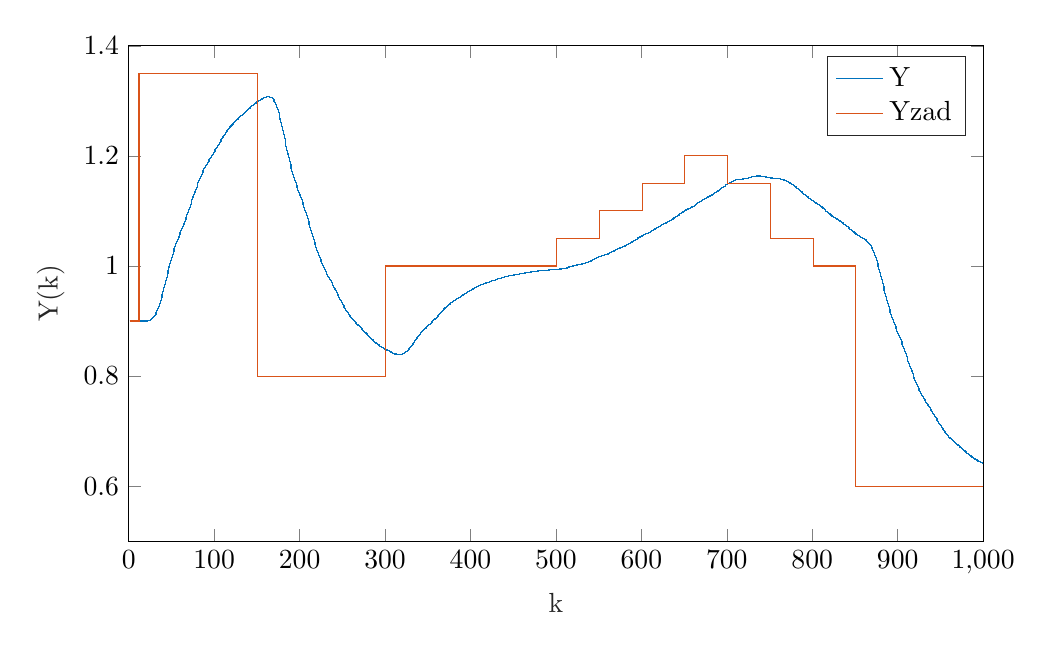
\begin{tikzpicture}

\begin{axis}[%
width=4.272in,
height=2.477in,
at={(0.717in,0.437in)},
scale only axis,
xmin=0,
xmax=1000,
xlabel style={font=\color{white!15!black}},
xlabel={k},
ymin=0.5,
ymax=1.4,
ylabel style={font=\color{white!15!black}},
ylabel={Y(k)},
axis background/.style={fill=white},
legend style={legend cell align=left, align=left, draw=white!15!black}
]
\addplot[const plot, color=mycolor1] table[row sep=crcr] {%
1	0.9\\
2	0.9\\
3	0.9\\
4	0.9\\
5	0.9\\
6	0.9\\
7	0.9\\
8	0.9\\
9	0.9\\
10	0.9\\
11	0.9\\
12	0.9\\
13	0.9\\
14	0.9\\
15	0.9\\
16	0.9\\
17	0.9\\
18	0.9\\
19	0.9\\
20	0.9\\
21	0.9\\
22	0.9003968325\\
23	0.90110505465075\\
24	0.901754499448244\\
25	0.902462381771257\\
26	0.903327432799628\\
27	0.904432123866198\\
28	0.90584465078664\\
29	0.907620702973639\\
30	0.909805039263915\\
31	0.912432890235655\\
32	0.915498096835601\\
33	0.918965853372063\\
34	0.922837193061285\\
35	0.927128134502026\\
36	0.931831863484165\\
37	0.936923734431968\\
38	0.942365468215513\\
39	0.948108657807613\\
40	0.954097679116409\\
41	0.960272091866446\\
42	0.966571366665219\\
43	0.97294065568034\\
44	0.979329694247744\\
45	0.985688442749354\\
46	0.991967881999957\\
47	0.998123300499065\\
48	1.00411656075767\\
49	1.00991755516541\\
50	1.01550502606484\\
51	1.0208668943165\\
52	1.0259999844607\\
53	1.03090892615053\\
54	1.03560478986773\\
55	1.04010429107047\\
56	1.04442934161618\\
57	1.04860630459408\\
58	1.05266486491142\\
59	1.05663669420945\\
60	1.0605540422755\\
61	1.06444835015091\\
62	1.06834897017567\\
63	1.07228209848007\\
64	1.07626998780362\\
65	1.08033038969881\\
66	1.08447613243709\\
67	1.08871482012883\\
68	1.09304869808435\\
69	1.09747471797913\\
70	1.10198480880132\\
71	1.10656634102768\\
72	1.11120275821343\\
73	1.11587433707758\\
74	1.12055902663016\\
75	1.12523332003065\\
76	1.12987312861239\\
77	1.13445463865313\\
78	1.13895513044294\\
79	1.14335373448336\\
80	1.14763209849147\\
81	1.15177494149719\\
82	1.1557704762483\\
83	1.15961068776104\\
84	1.16329146381875\\
85	1.16681258108326\\
86	1.17017755613573\\
87	1.17339337378769\\
88	1.17647010700276\\
89	1.17942044510106\\
90	1.18225914955358\\
91	1.18500245899432\\
92	1.18766746662559\\
93	1.19027149370736\\
94	1.19283148214764\\
95	1.19536342734718\\
96	1.1978818696875\\
97	1.20039945985026\\
98	1.20292660984184\\
99	1.20547123822702\\
100	1.2080386145976\\
101	1.21063130471987\\
102	1.21324921421263\\
103	1.21588972514576\\
104	1.21854791678215\\
105	1.22121685897705\\
106	1.22388796462404\\
107	1.22655138605161\\
108	1.2291964394166\\
109	1.23181204087031\\
110	1.23438713855422\\
111	1.2369111252862\\
112	1.23937421809208\\
113	1.24176779247258\\
114	1.24408466140287\\
115	1.24631929145305\\
116	1.24846795098764\\
117	1.2505287880408\\
118	1.2525018380675\\
119	1.25438896424786\\
120	1.25619373529506\\
121	1.25792124771947\\
122	1.25957790117795\\
123	1.26117113684122\\
124	1.26270914961122\\
125	1.26420058549763\\
126	1.26565423551553\\
127	1.26707873711107\\
128	1.26848229338989\\
129	1.2698724193567\\
130	1.27125572302791\\
131	1.27263772771127\\
132	1.27402274002252\\
133	1.27541376639511\\
134	1.27681247900324\\
135	1.27821923022645\\
136	1.27963311309799\\
137	1.28105206365459\\
138	1.28247299979045\\
139	1.28389199015027\\
140	1.285304445803\\
141	1.28670532693611\\
142	1.2880893566037\\
143	1.28945123364788\\
144	1.29078583727327\\
145	1.29208841636796\\
146	1.29335475749583\\
147	1.29458132649851\\
148	1.29576537979462\\
149	1.29690504270447\\
150	1.29799935341126\\
151	1.29904827244758\\
152	1.30005265882428\\
153	1.30101421505558\\
154	1.30193540434301\\
155	1.30281934403149\\
156	1.30366968011989\\
157	1.30449044807919\\
158	1.30528592549637\\
159	1.30606048211984\\
160	1.30681843273953\\
161	1.30716369682455\\
162	1.30717941725438\\
163	1.30722458102453\\
164	1.30716381414196\\
165	1.30688317044968\\
166	1.30628742896576\\
167	1.30529770217837\\
168	1.30384932587905\\
169	1.3018900031321\\
170	1.2993781767954\\
171	1.29631499574341\\
172	1.2927319090087\\
173	1.2886269424304\\
174	1.28398656026348\\
175	1.2788234391972\\
176	1.27317069285459\\
177	1.26707704408256\\
178	1.26060280915345\\
179	1.25381657523541\\
180	1.24679246780261\\
181	1.23960513258249\\
182	1.23232366515491\\
183	1.22501234716547\\
184	1.21773453022157\\
185	1.21055133104061\\
186	1.20351794537139\\
187	1.19668112903149\\
188	1.19007760151277\\
189	1.18373317014001\\
190	1.17766240879857\\
191	1.1718689880777\\
192	1.16634687067229\\
193	1.16108181655011\\
194	1.15605237449859\\
195	1.15123058867484\\
196	1.14658305274622\\
197	1.14207237455282\\
198	1.13765885013809\\
199	1.13330219926585\\
200	1.12896325677001\\
201	1.12460552784681\\
202	1.12019649736667\\
203	1.1157086215278\\
204	1.11112004815648\\
205	1.10641515354477\\
206	1.10158490527865\\
207	1.09662700428\\
208	1.0915457746403\\
209	1.08635180023695\\
210	1.08106132727517\\
211	1.07569546592208\\
212	1.07027923752917\\
213	1.0648405244653\\
214	1.05940897646577\\
215	1.05401491185706\\
216	1.04868824109481\\
217	1.04345744096653\\
218	1.03834861185122\\
219	1.0333846504378\\
220	1.02858456628647\\
221	1.02396296422117\\
222	1.01952970649721\\
223	1.01528975940691\\
224	1.01124321991638\\
225	1.00738551114763\\
226	1.00370773142582\\
227	1.00019713861747\\
228	0.99683774830098\\
229	0.993611021036291\\
230	0.990496611290706\\
231	0.987473148899105\\
232	0.984519023523776\\
233	0.981613143560161\\
234	0.978735643274665\\
235	0.975868515342502\\
236	0.97299614989132\\
237	0.970105765306768\\
238	0.967187720337565\\
239	0.964235701468817\\
240	0.961246784068318\\
241	0.958221370319641\\
242	0.955163011260938\\
243	0.952078124157511\\
244	0.948975619765714\\
245	0.945866456655265\\
246	0.94276314158254\\
247	0.939679195955599\\
248	0.936628608741493\\
249	0.93362529577704\\
250	0.930682584392817\\
251	0.927812740593989\\
252	0.92502655382839\\
253	0.922332991702936\\
254	0.919738933997245\\
255	0.917248992097394\\
256	0.91486541666791\\
257	0.912588093123838\\
258	0.910414621370712\\
259	0.908340473446145\\
260	0.906359220206614\\
261	0.904462816127511\\
262	0.902641929679672\\
263	0.900886305650784\\
264	0.8991851452154\\
265	0.897527489522673\\
266	0.895902593045374\\
267	0.894300273878\\
268	0.892711229530689\\
269	0.891127308472649\\
270	0.889541729658373\\
271	0.887949244441043\\
272	0.886346237555857\\
273	0.884730766156806\\
274	0.88310253813116\\
275	0.881462833019366\\
276	0.879814370764858\\
277	0.878161135149582\\
278	0.876508160089889\\
279	0.874861287940593\\
280	0.873226909562449\\
281	0.871611696144242\\
282	0.870022332642392\\
283	0.868465262228174\\
284	0.866946450346648\\
285	0.865471175933068\\
286	0.864043856050893\\
287	0.862667908765514\\
288	0.861345657508032\\
289	0.860078278573851\\
290	0.858865791800825\\
291	0.857707092937426\\
292	0.856600024794666\\
293	0.855541483021535\\
294	0.854527551290118\\
295	0.853553659852368\\
296	0.852614760855281\\
297	0.851705513484875\\
298	0.850820471952338\\
299	0.84995426952895\\
300	0.849101792262645\\
301	0.848258336643261\\
302	0.847419746294486\\
303	0.846582523721994\\
304	0.84574391419954\\
305	0.844901959986352\\
306	0.844055524198045\\
307	0.843204284758678\\
308	0.842348699905252\\
309	0.841489947663514\\
310	0.840629842535724\\
311	0.840169094662738\\
312	0.840027359635076\\
313	0.839805903831571\\
314	0.839567209155041\\
315	0.83936480474152\\
316	0.839244206365335\\
317	0.839243750798437\\
318	0.839395340436324\\
319	0.839725111766168\\
320	0.840254039536307\\
321	0.840965251242341\\
322	0.841815990385479\\
323	0.842804380409815\\
324	0.843952805469557\\
325	0.845270429284305\\
326	0.846755821961687\\
327	0.848399199457051\\
328	0.850184327694026\\
329	0.852090136165507\\
330	0.854092079575684\\
331	0.856166053544525\\
332	0.858293559373643\\
333	0.860459927998672\\
334	0.862648812483973\\
335	0.864841570203845\\
336	0.867019426091502\\
337	0.869165057096226\\
338	0.871263707431921\\
339	0.873303926457666\\
340	0.875278006001206\\
341	0.877181949883109\\
342	0.879014709072526\\
343	0.880777223160516\\
344	0.882472141796327\\
345	0.884104055543816\\
346	0.885679576426447\\
347	0.887207109824139\\
348	0.888696427994394\\
349	0.890158129663874\\
350	0.891603049252957\\
351	0.893041681803541\\
352	0.894483719627462\\
353	0.895937764786653\\
354	0.897411160909335\\
355	0.898909838051168\\
356	0.900438141685211\\
357	0.901998684545975\\
358	0.90359226015397\\
359	0.905217837966332\\
360	0.906872646603919\\
361	0.908552340683483\\
362	0.910251234068291\\
363	0.911962570966477\\
364	0.913678808404027\\
365	0.915391899148136\\
366	0.917093575864466\\
367	0.918775636276858\\
368	0.920430222821914\\
369	0.922050086094013\\
370	0.923628820126828\\
371	0.925161058368271\\
372	0.926642621853169\\
373	0.928070615443676\\
374	0.929443472725517\\
375	0.930760953011266\\
376	0.93202409432847\\
377	0.933235125828997\\
378	0.934397343260897\\
379	0.935514952183391\\
380	0.936592885001724\\
381	0.937636599219598\\
382	0.938651865245467\\
383	0.93964455239024\\
384	0.940620421246598\\
385	0.941584929632738\\
386	0.942543058110608\\
387	0.943499160027043\\
388	0.944456840079157\\
389	0.945418864441198\\
390	0.946387104412926\\
391	0.947362514345214\\
392	0.948345143313419\\
393	0.949334178730906\\
394	0.950328018934164\\
395	0.951324370821061\\
396	0.9523203679239\\
397	0.953312703830763\\
398	0.954297775593714\\
399	0.955271831656608\\
400	0.956231118895027\\
401	0.957172023592017\\
402	0.95809120157877\\
403	0.958985693341087\\
404	0.959853020607133\\
405	0.960691261752121\\
406	0.961499104236219\\
407	0.962275873190419\\
408	0.9630215361472\\
409	0.963736684751766\\
410	0.96442249506354\\
411	0.965080668745633\\
412	0.965713358022552\\
413	0.966323077745515\\
414	0.966912608226528\\
415	0.967484892678643\\
416	0.968042933129712\\
417	0.968589688566427\\
418	0.969127978825942\\
419	0.969660397399219\\
420	0.970189235861091\\
421	0.970716422116399\\
422	0.971243474070611\\
423	0.971771469719207\\
424	0.972301034025811\\
425	0.972832342347339\\
426	0.973365139586878\\
427	0.973898773731139\\
428	0.974432241975527\\
429	0.974964247269264\\
430	0.975493262835007\\
431	0.976017602037695\\
432	0.97653549089826\\
433	0.977045140567746\\
434	0.97754481719178\\
435	0.978032906796037\\
436	0.978507973099932\\
437	0.978968806504891\\
438	0.979414462890818\\
439	0.979844291273657\\
440	0.980257949812176\\
441	0.980655410087131\\
442	0.98103694999534\\
443	0.981403135990794\\
444	0.981754795752179\\
445	0.982092982650503\\
446	0.982418933623735\\
447	0.982734022231702\\
448	0.983039708760909\\
449	0.983337489274906\\
450	0.983628845463454\\
451	0.983915197037351\\
452	0.98419785825193\\
453	0.984477999929074\\
454	0.984756618094831\\
455	0.985034510067923\\
456	0.985312258534895\\
457	0.985590223841668\\
458	0.985868544430038\\
459	0.986147145061628\\
460	0.98642575221052\\
461	0.986703915777452\\
462	0.986981036089827\\
463	0.987256395007808\\
464	0.987529189860735\\
465	0.987798568891391\\
466	0.988063666887806\\
467	0.988323639731228\\
468	0.988577696680858\\
469	0.988825129345951\\
470	0.989065336457574\\
471	0.989297843738771\\
472	0.989522318375325\\
473	0.989738577801861\\
474	0.989946592731781\\
475	0.990146484566763\\
476	0.990338517515298\\
477	0.990523085923603\\
478	0.990700697470936\\
479	0.990871953000652\\
480	0.991037523845198\\
481	0.991198127556078\\
482	0.991354502968001\\
483	0.99150738551097\\
484	0.991657483636728\\
485	0.991805457149996\\
486	0.99195189813403\\
487	0.992097315038895\\
488	0.992242120364734\\
489	0.992386622226472\\
490	0.992531019936621\\
491	0.992675403594489\\
492	0.992819757528406\\
493	0.992963967307301\\
494	0.993107829923245\\
495	0.993251066650795\\
496	0.993393338014796\\
497	0.993534260247401\\
498	0.993673422588261\\
499	0.993810404779147\\
500	0.993944794124629\\
501	0.99407620153232\\
502	0.994204276007057\\
503	0.994328717150409\\
504	0.994449285306534\\
505	0.994565809094043\\
506	0.994678190167261\\
507	0.994786405155133\\
508	0.994890504828404\\
509	0.994990610641852\\
510	0.995086908885376\\
511	0.995576320281363\\
512	0.996373384114822\\
513	0.997056856627257\\
514	0.997652839785233\\
515	0.998184012720492\\
516	0.998670007498053\\
517	0.999127744934178\\
518	0.999571734880995\\
519	1.00001434495842\\
520	1.00046604130442\\
521	1.00090250944675\\
522	1.00127650821095\\
523	1.0015858198777\\
524	1.00185870519926\\
525	1.00211644344964\\
526	1.00237451129508\\
527	1.00264359443392\\
528	1.00293045372561\\
529	1.00323866481912\\
530	1.00356924790285\\
531	1.00392396324233\\
532	1.00430993647707\\
533	1.00473730119126\\
534	1.00521289410927\\
535	1.00573874175239\\
536	1.00631352098964\\
537	1.00693371374279\\
538	1.00759450858742\\
539	1.00829049389687\\
540	1.00901618023572\\
541	1.00976615340582\\
542	1.01053456799302\\
543	1.01131451329682\\
544	1.01209814152972\\
545	1.01287740668452\\
546	1.0136447383078\\
547	1.01439344764917\\
548	1.01511793444369\\
549	1.01581374868606\\
550	1.01647755031866\\
551	1.01710701960353\\
552	1.01770080634101\\
553	1.01825857732303\\
554	1.01878110040905\\
555	1.01927025124573\\
556	1.01972890636205\\
557	1.02016075941615\\
558	1.02057010446154\\
559	1.02096161646853\\
560	1.02134014894019\\
561	1.02210452711472\\
562	1.0231686533107\\
563	1.02411388033609\\
564	1.02497152632599\\
565	1.02576872843422\\
566	1.02652873592204\\
567	1.02727119274802\\
568	1.02801241990539\\
569	1.02876570092291\\
570	1.02954156963095\\
571	1.0303152279108\\
572	1.0310388789943\\
573	1.0317096173736\\
574	1.0323544237142\\
575	1.03299261216525\\
576	1.03363719623706\\
577	1.03429608179113\\
578	1.03497310437641\\
579	1.03566892538143\\
580	1.03638179985561\\
581	1.03711097021104\\
582	1.03786131833729\\
583	1.03864100027169\\
584	1.03945517760363\\
585	1.04030458173921\\
586	1.04118703782354\\
587	1.0420986482806\\
588	1.04303469293783\\
589	1.04399029493723\\
590	1.04496089494533\\
591	1.04594234152182\\
592	1.04693031770527\\
593	1.04791964447353\\
594	1.04890434954974\\
595	1.04987834266631\\
596	1.05083601969436\\
597	1.05177259750311\\
598	1.05268425308141\\
599	1.05356812540787\\
600	1.05442222602796\\
601	1.05524531299143\\
602	1.05603681669851\\
603	1.05679687588109\\
604	1.05752642048665\\
605	1.05822718673863\\
606	1.05890162816246\\
607	1.05955275920072\\
608	1.06018397437369\\
609	1.06079887163916\\
610	1.06140109777379\\
611	1.06238815529502\\
612	1.06367267808548\\
613	1.06483479509767\\
614	1.06590458609383\\
615	1.06690806065741\\
616	1.06786748757226\\
617	1.06880170721111\\
618	1.06972643631653\\
619	1.0706545679902\\
620	1.07159646572185\\
621	1.07252738232499\\
622	1.07339977939622\\
623	1.07421119225364\\
624	1.07498920795452\\
625	1.07575389159591\\
626	1.07651912025515\\
627	1.07729374153833\\
628	1.07808257524797\\
629	1.07888727392648\\
630	1.07970705637811\\
631	1.08054206928726\\
632	1.08139801088139\\
633	1.08228374254525\\
634	1.08320500228119\\
635	1.08416295539202\\
636	1.08515571003377\\
637	1.08617949822132\\
638	1.08722957906351\\
639	1.0883009130564\\
640	1.08938864940792\\
641	1.09048823359354\\
642	1.09159485441299\\
643	1.09270277022996\\
644	1.09380540185966\\
645	1.09489603238126\\
646	1.09596843550646\\
647	1.09701723353714\\
648	1.09803805764719\\
649	1.09902756828703\\
650	1.0999833811087\\
651	1.10090395264316\\
652	1.10178851400379\\
653	1.10263711072739\\
654	1.10345068556976\\
655	1.10423108971657\\
656	1.10498098649525\\
657	1.10570368460722\\
658	1.10640294432696\\
659	1.10708278588701\\
660	1.10774731848689\\
661	1.10879426684647\\
662	1.11013625476138\\
663	1.11135373743873\\
664	1.11247740266507\\
665	1.11353380841378\\
666	1.11454570224341\\
667	1.11553232585545\\
668	1.11650971445948\\
669	1.11749099392267\\
670	1.1184866745911\\
671	1.11947209456598\\
672	1.12039978281921\\
673	1.12126731604091\\
674	1.12210224887935\\
675	1.12292452910398\\
676	1.12374784895551\\
677	1.12458082097511\\
678	1.12542799649262\\
679	1.12629074219102\\
680	1.1271679885211\\
681	1.12805960294725\\
682	1.12897101871664\\
683	1.12991084840482\\
684	1.13088460379443\\
685	1.13189325717508\\
686	1.13293476610728\\
687	1.13400526012467\\
688	1.13509994650245\\
689	1.13621378429167\\
690	1.13734196898248\\
691	1.13848003555344\\
692	1.13962330012502\\
693	1.14076618074463\\
694	1.14190228463933\\
695	1.14302510151463\\
696	1.1441286243791\\
697	1.1452076994052\\
698	1.14625817813512\\
699	1.1472769302977\\
700	1.14826176300142\\
701	1.1492113007963\\
702	1.15012491499655\\
703	1.15100276034006\\
704	1.15184585571573\\
705	1.1526560944107\\
706	1.15343614802474\\
707	1.15418930110183\\
708	1.15491925987001\\
709	1.15562996417528\\
710	1.15632542085964\\
711	1.15660953296027\\
712	1.15656562739792\\
713	1.15661695467116\\
714	1.15674276891108\\
715	1.15692504397472\\
716	1.15714802462289\\
717	1.15739784291573\\
718	1.15766220131747\\
719	1.15793011813117\\
720	1.15819172753006\\
721	1.15847150016088\\
722	1.15881694305253\\
723	1.15923053228696\\
724	1.15968365629161\\
725	1.1601539234925\\
726	1.16062416814294\\
727	1.16108161656035\\
728	1.16151718832924\\
729	1.16192490959913\\
730	1.1623014186716\\
731	1.1626427627249\\
732	1.16293978402222\\
733	1.16318045408291\\
734	1.16335621669888\\
735	1.16346359664284\\
736	1.16350282346908\\
737	1.16347672519449\\
738	1.16338984362053\\
739	1.16324773134106\\
740	1.163056397555\\
741	1.16282210804564\\
742	1.16255184080787\\
743	1.16225387495435\\
744	1.16193762008565\\
745	1.16161282781298\\
746	1.16128885812461\\
747	1.16097420775358\\
748	1.16067623811486\\
749	1.16040105304662\\
750	1.16015348687908\\
751	1.15993715228771\\
752	1.15975446034756\\
753	1.15960655226226\\
754	1.15949320284716\\
755	1.15941280941183\\
756	1.15936250305687\\
757	1.15933834616354\\
758	1.15933557188196\\
759	1.15934883425454\\
760	1.15937244746529\\
761	1.15900607376211\\
762	1.15833390341491\\
763	1.157766928442\\
764	1.15726160581972\\
765	1.15678047243207\\
766	1.15629166314418\\
767	1.15576845944938\\
768	1.15518885488097\\
769	1.15453513065448\\
770	1.15379343983219\\
771	1.15298631693775\\
772	1.15216029934633\\
773	1.15131842387498\\
774	1.15043591462256\\
775	1.14949773433263\\
776	1.14849672806443\\
777	1.14743201403219\\
778	1.14630759444943\\
779	1.14513116345229\\
780	1.14391309205334\\
781	1.14266282588095\\
782	1.14138405286393\\
783	1.14007687579086\\
784	1.13874381743319\\
785	1.13739096119269\\
786	1.13602619733521\\
787	1.13465790136206\\
788	1.13329396838876\\
789	1.13194113837472\\
790	1.13060455643133\\
791	1.12928774967432\\
792	1.12799329248697\\
793	1.12672361640726\\
794	1.12548108141797\\
795	1.12426747371202\\
796	1.12308360208697\\
797	1.12192917631291\\
798	1.12080287991332\\
799	1.11970256885595\\
800	1.11862554336144\\
801	1.11756883382064\\
802	1.1165294097582\\
803	1.11550425217048\\
804	1.11449035090926\\
805	1.11348473943144\\
806	1.11248460083501\\
807	1.11148740806793\\
808	1.11049105718672\\
809	1.10949396858202\\
810	1.1084951429369\\
811	1.10710085710149\\
812	1.10540272560453\\
813	1.10382439704228\\
814	1.10233945785245\\
815	1.10092555673665\\
816	1.09956393938571\\
817	1.09823901149092\\
818	1.09693792473891\\
819	1.09565018629839\\
820	1.09436729538197\\
821	1.09311522578388\\
822	1.09194203083433\\
823	1.09085003884519\\
824	1.08981097364837\\
825	1.08880358084663\\
826	1.0878123445037\\
827	1.08682639548319\\
828	1.08583858950236\\
829	1.08484473542966\\
830	1.08384295586982\\
831	1.08283042539599\\
832	1.08179885254763\\
833	1.08073696622068\\
834	1.0796368794415\\
835	1.07849559783094\\
836	1.07731355050408\\
837	1.07609344275047\\
838	1.074839372482\\
839	1.07355616104324\\
840	1.07224885647259\\
841	1.07092260231086\\
842	1.06958315289201\\
843	1.0682374967167\\
844	1.0668937037547\\
845	1.06556016022923\\
846	1.06424487209224\\
847	1.06295503833647\\
848	1.06169682351523\\
849	1.0604752737494\\
850	1.05929433277565\\
851	1.05815690557293\\
852	1.05706488288663\\
853	1.05601906989174\\
854	1.05501908305764\\
855	1.05406332999805\\
856	1.05314910792501\\
857	1.0522727830289\\
858	1.0514300064048\\
859	1.05061593612723\\
860	1.04982544564154\\
861	1.04866006194682\\
862	1.04720675699953\\
863	1.04583915201055\\
864	1.04444483292963\\
865	1.04292876302134\\
866	1.04121139574632\\
867	1.0392269724676\\
868	1.03692197637707\\
869	1.03425372271224\\
870	1.03118907127479\\
871	1.02773605986978\\
872	1.0239306788736\\
873	1.0197720691455\\
874	1.01524322831835\\
875	1.0103489406592\\
876	1.00511104002655\\
877	0.999564401455219\\
878	0.993753565771211\\
879	0.987729914538255\\
880	0.981549323160261\\
881	0.975267491456203\\
882	0.96893428242139\\
883	0.962594984024355\\
884	0.956294853322811\\
885	0.95007849318461\\
886	0.943986691587205\\
887	0.93805423455346\\
888	0.932308497231893\\
889	0.926768649650635\\
890	0.921445340872772\\
891	0.916340976806125\\
892	0.911450808238994\\
893	0.906764263645407\\
894	0.902265688195684\\
895	0.897934711556627\\
896	0.893746895133604\\
897	0.889674755244686\\
898	0.885688990620384\\
899	0.881759786331988\\
900	0.877858101313884\\
901	0.873956855501901\\
902	0.870031912293237\\
903	0.866062790490992\\
904	0.862033159520349\\
905	0.857931214455777\\
906	0.853749947312385\\
907	0.849487270131541\\
908	0.845145955558932\\
909	0.84073338738237\\
910	0.836261131649344\\
911	0.831744352136894\\
912	0.827201107038398\\
913	0.822651574187706\\
914	0.818117248789103\\
915	0.813620141617379\\
916	0.809181994337698\\
917	0.804823529652822\\
918	0.800563758943257\\
919	0.7964193716131\\
920	0.792404228186671\\
921	0.788528974721117\\
922	0.784800789892824\\
923	0.781223268538993\\
924	0.777796437951791\\
925	0.774516897955673\\
926	0.771378073162333\\
927	0.76837056416608\\
928	0.765482582427319\\
929	0.762700451198557\\
930	0.760009152682474\\
931	0.757392900138492\\
932	0.754835713139305\\
933	0.752321974791951\\
934	0.749836951486375\\
935	0.747367258334212\\
936	0.744901256450578\\
937	0.742429371293228\\
938	0.739944324358326\\
939	0.737441273705462\\
940	0.73491786205511\\
941	0.732374174491128\\
942	0.729812610978711\\
943	0.72723768181921\\
944	0.724655736650958\\
945	0.722074639548534\\
946	0.719503404120612\\
947	0.716951803273966\\
948	0.714429968540231\\
949	0.711947993588959\\
950	0.709515555801358\\
951	0.707141568583377\\
952	0.704833875497243\\
953	0.702598995349443\\
954	0.700441925171891\\
955	0.698366005668534\\
956	0.696372851274094\\
957	0.694462344581607\\
958	0.692632692624408\\
959	0.690880540417061\\
960	0.689201135328303\\
961	0.687588534328345\\
962	0.686035844964175\\
963	0.684535490099561\\
964	0.683079486027715\\
965	0.68165972352496\\
966	0.680268241748796\\
967	0.678897485564674\\
968	0.677540537872084\\
969	0.676191319743302\\
970	0.67484475263212\\
971	0.673496878496058\\
972	0.672144935342448\\
973	0.670787387394415\\
974	0.669423910716804\\
975	0.6680553366876\\
976	0.666683557096194\\
977	0.66531139585244\\
978	0.663942453265141\\
979	0.662580929570544\\
980	0.661231434845904\\
981	0.659898792625496\\
982	0.658587844451669\\
983	0.657303262255805\\
984	0.656049374895924\\
985	0.654830014408904\\
986	0.653648386601519\\
987	0.652506969545916\\
988	0.651407442404593\\
989	0.650350645831398\\
990	0.649336574021993\\
991	0.648364397360974\\
992	0.647432513571419\\
993	0.646538624349309\\
994	0.645679833687972\\
995	0.644852763487643\\
996	0.644053681617327\\
997	0.643278637357637\\
998	0.642523599104896\\
999	0.641784589352077\\
1000	0.641057812268653\\
};
\addlegendentry{Y}

\addplot[const plot, color=mycolor2] table[row sep=crcr] {%
1	0.9\\
2	0.9\\
3	0.9\\
4	0.9\\
5	0.9\\
6	0.9\\
7	0.9\\
8	0.9\\
9	0.9\\
10	0.9\\
11	0.9\\
12	1.35\\
13	1.35\\
14	1.35\\
15	1.35\\
16	1.35\\
17	1.35\\
18	1.35\\
19	1.35\\
20	1.35\\
21	1.35\\
22	1.35\\
23	1.35\\
24	1.35\\
25	1.35\\
26	1.35\\
27	1.35\\
28	1.35\\
29	1.35\\
30	1.35\\
31	1.35\\
32	1.35\\
33	1.35\\
34	1.35\\
35	1.35\\
36	1.35\\
37	1.35\\
38	1.35\\
39	1.35\\
40	1.35\\
41	1.35\\
42	1.35\\
43	1.35\\
44	1.35\\
45	1.35\\
46	1.35\\
47	1.35\\
48	1.35\\
49	1.35\\
50	1.35\\
51	1.35\\
52	1.35\\
53	1.35\\
54	1.35\\
55	1.35\\
56	1.35\\
57	1.35\\
58	1.35\\
59	1.35\\
60	1.35\\
61	1.35\\
62	1.35\\
63	1.35\\
64	1.35\\
65	1.35\\
66	1.35\\
67	1.35\\
68	1.35\\
69	1.35\\
70	1.35\\
71	1.35\\
72	1.35\\
73	1.35\\
74	1.35\\
75	1.35\\
76	1.35\\
77	1.35\\
78	1.35\\
79	1.35\\
80	1.35\\
81	1.35\\
82	1.35\\
83	1.35\\
84	1.35\\
85	1.35\\
86	1.35\\
87	1.35\\
88	1.35\\
89	1.35\\
90	1.35\\
91	1.35\\
92	1.35\\
93	1.35\\
94	1.35\\
95	1.35\\
96	1.35\\
97	1.35\\
98	1.35\\
99	1.35\\
100	1.35\\
101	1.35\\
102	1.35\\
103	1.35\\
104	1.35\\
105	1.35\\
106	1.35\\
107	1.35\\
108	1.35\\
109	1.35\\
110	1.35\\
111	1.35\\
112	1.35\\
113	1.35\\
114	1.35\\
115	1.35\\
116	1.35\\
117	1.35\\
118	1.35\\
119	1.35\\
120	1.35\\
121	1.35\\
122	1.35\\
123	1.35\\
124	1.35\\
125	1.35\\
126	1.35\\
127	1.35\\
128	1.35\\
129	1.35\\
130	1.35\\
131	1.35\\
132	1.35\\
133	1.35\\
134	1.35\\
135	1.35\\
136	1.35\\
137	1.35\\
138	1.35\\
139	1.35\\
140	1.35\\
141	1.35\\
142	1.35\\
143	1.35\\
144	1.35\\
145	1.35\\
146	1.35\\
147	1.35\\
148	1.35\\
149	1.35\\
150	1.35\\
151	0.8\\
152	0.8\\
153	0.8\\
154	0.8\\
155	0.8\\
156	0.8\\
157	0.8\\
158	0.8\\
159	0.8\\
160	0.8\\
161	0.8\\
162	0.8\\
163	0.8\\
164	0.8\\
165	0.8\\
166	0.8\\
167	0.8\\
168	0.8\\
169	0.8\\
170	0.8\\
171	0.8\\
172	0.8\\
173	0.8\\
174	0.8\\
175	0.8\\
176	0.8\\
177	0.8\\
178	0.8\\
179	0.8\\
180	0.8\\
181	0.8\\
182	0.8\\
183	0.8\\
184	0.8\\
185	0.8\\
186	0.8\\
187	0.8\\
188	0.8\\
189	0.8\\
190	0.8\\
191	0.8\\
192	0.8\\
193	0.8\\
194	0.8\\
195	0.8\\
196	0.8\\
197	0.8\\
198	0.8\\
199	0.8\\
200	0.8\\
201	0.8\\
202	0.8\\
203	0.8\\
204	0.8\\
205	0.8\\
206	0.8\\
207	0.8\\
208	0.8\\
209	0.8\\
210	0.8\\
211	0.8\\
212	0.8\\
213	0.8\\
214	0.8\\
215	0.8\\
216	0.8\\
217	0.8\\
218	0.8\\
219	0.8\\
220	0.8\\
221	0.8\\
222	0.8\\
223	0.8\\
224	0.8\\
225	0.8\\
226	0.8\\
227	0.8\\
228	0.8\\
229	0.8\\
230	0.8\\
231	0.8\\
232	0.8\\
233	0.8\\
234	0.8\\
235	0.8\\
236	0.8\\
237	0.8\\
238	0.8\\
239	0.8\\
240	0.8\\
241	0.8\\
242	0.8\\
243	0.8\\
244	0.8\\
245	0.8\\
246	0.8\\
247	0.8\\
248	0.8\\
249	0.8\\
250	0.8\\
251	0.8\\
252	0.8\\
253	0.8\\
254	0.8\\
255	0.8\\
256	0.8\\
257	0.8\\
258	0.8\\
259	0.8\\
260	0.8\\
261	0.8\\
262	0.8\\
263	0.8\\
264	0.8\\
265	0.8\\
266	0.8\\
267	0.8\\
268	0.8\\
269	0.8\\
270	0.8\\
271	0.8\\
272	0.8\\
273	0.8\\
274	0.8\\
275	0.8\\
276	0.8\\
277	0.8\\
278	0.8\\
279	0.8\\
280	0.8\\
281	0.8\\
282	0.8\\
283	0.8\\
284	0.8\\
285	0.8\\
286	0.8\\
287	0.8\\
288	0.8\\
289	0.8\\
290	0.8\\
291	0.8\\
292	0.8\\
293	0.8\\
294	0.8\\
295	0.8\\
296	0.8\\
297	0.8\\
298	0.8\\
299	0.8\\
300	0.8\\
301	1\\
302	1\\
303	1\\
304	1\\
305	1\\
306	1\\
307	1\\
308	1\\
309	1\\
310	1\\
311	1\\
312	1\\
313	1\\
314	1\\
315	1\\
316	1\\
317	1\\
318	1\\
319	1\\
320	1\\
321	1\\
322	1\\
323	1\\
324	1\\
325	1\\
326	1\\
327	1\\
328	1\\
329	1\\
330	1\\
331	1\\
332	1\\
333	1\\
334	1\\
335	1\\
336	1\\
337	1\\
338	1\\
339	1\\
340	1\\
341	1\\
342	1\\
343	1\\
344	1\\
345	1\\
346	1\\
347	1\\
348	1\\
349	1\\
350	1\\
351	1\\
352	1\\
353	1\\
354	1\\
355	1\\
356	1\\
357	1\\
358	1\\
359	1\\
360	1\\
361	1\\
362	1\\
363	1\\
364	1\\
365	1\\
366	1\\
367	1\\
368	1\\
369	1\\
370	1\\
371	1\\
372	1\\
373	1\\
374	1\\
375	1\\
376	1\\
377	1\\
378	1\\
379	1\\
380	1\\
381	1\\
382	1\\
383	1\\
384	1\\
385	1\\
386	1\\
387	1\\
388	1\\
389	1\\
390	1\\
391	1\\
392	1\\
393	1\\
394	1\\
395	1\\
396	1\\
397	1\\
398	1\\
399	1\\
400	1\\
401	1\\
402	1\\
403	1\\
404	1\\
405	1\\
406	1\\
407	1\\
408	1\\
409	1\\
410	1\\
411	1\\
412	1\\
413	1\\
414	1\\
415	1\\
416	1\\
417	1\\
418	1\\
419	1\\
420	1\\
421	1\\
422	1\\
423	1\\
424	1\\
425	1\\
426	1\\
427	1\\
428	1\\
429	1\\
430	1\\
431	1\\
432	1\\
433	1\\
434	1\\
435	1\\
436	1\\
437	1\\
438	1\\
439	1\\
440	1\\
441	1\\
442	1\\
443	1\\
444	1\\
445	1\\
446	1\\
447	1\\
448	1\\
449	1\\
450	1\\
451	1\\
452	1\\
453	1\\
454	1\\
455	1\\
456	1\\
457	1\\
458	1\\
459	1\\
460	1\\
461	1\\
462	1\\
463	1\\
464	1\\
465	1\\
466	1\\
467	1\\
468	1\\
469	1\\
470	1\\
471	1\\
472	1\\
473	1\\
474	1\\
475	1\\
476	1\\
477	1\\
478	1\\
479	1\\
480	1\\
481	1\\
482	1\\
483	1\\
484	1\\
485	1\\
486	1\\
487	1\\
488	1\\
489	1\\
490	1\\
491	1\\
492	1\\
493	1\\
494	1\\
495	1\\
496	1\\
497	1\\
498	1\\
499	1\\
500	1\\
501	1.05\\
502	1.05\\
503	1.05\\
504	1.05\\
505	1.05\\
506	1.05\\
507	1.05\\
508	1.05\\
509	1.05\\
510	1.05\\
511	1.05\\
512	1.05\\
513	1.05\\
514	1.05\\
515	1.05\\
516	1.05\\
517	1.05\\
518	1.05\\
519	1.05\\
520	1.05\\
521	1.05\\
522	1.05\\
523	1.05\\
524	1.05\\
525	1.05\\
526	1.05\\
527	1.05\\
528	1.05\\
529	1.05\\
530	1.05\\
531	1.05\\
532	1.05\\
533	1.05\\
534	1.05\\
535	1.05\\
536	1.05\\
537	1.05\\
538	1.05\\
539	1.05\\
540	1.05\\
541	1.05\\
542	1.05\\
543	1.05\\
544	1.05\\
545	1.05\\
546	1.05\\
547	1.05\\
548	1.05\\
549	1.05\\
550	1.05\\
551	1.1\\
552	1.1\\
553	1.1\\
554	1.1\\
555	1.1\\
556	1.1\\
557	1.1\\
558	1.1\\
559	1.1\\
560	1.1\\
561	1.1\\
562	1.1\\
563	1.1\\
564	1.1\\
565	1.1\\
566	1.1\\
567	1.1\\
568	1.1\\
569	1.1\\
570	1.1\\
571	1.1\\
572	1.1\\
573	1.1\\
574	1.1\\
575	1.1\\
576	1.1\\
577	1.1\\
578	1.1\\
579	1.1\\
580	1.1\\
581	1.1\\
582	1.1\\
583	1.1\\
584	1.1\\
585	1.1\\
586	1.1\\
587	1.1\\
588	1.1\\
589	1.1\\
590	1.1\\
591	1.1\\
592	1.1\\
593	1.1\\
594	1.1\\
595	1.1\\
596	1.1\\
597	1.1\\
598	1.1\\
599	1.1\\
600	1.1\\
601	1.15\\
602	1.15\\
603	1.15\\
604	1.15\\
605	1.15\\
606	1.15\\
607	1.15\\
608	1.15\\
609	1.15\\
610	1.15\\
611	1.15\\
612	1.15\\
613	1.15\\
614	1.15\\
615	1.15\\
616	1.15\\
617	1.15\\
618	1.15\\
619	1.15\\
620	1.15\\
621	1.15\\
622	1.15\\
623	1.15\\
624	1.15\\
625	1.15\\
626	1.15\\
627	1.15\\
628	1.15\\
629	1.15\\
630	1.15\\
631	1.15\\
632	1.15\\
633	1.15\\
634	1.15\\
635	1.15\\
636	1.15\\
637	1.15\\
638	1.15\\
639	1.15\\
640	1.15\\
641	1.15\\
642	1.15\\
643	1.15\\
644	1.15\\
645	1.15\\
646	1.15\\
647	1.15\\
648	1.15\\
649	1.15\\
650	1.15\\
651	1.2\\
652	1.2\\
653	1.2\\
654	1.2\\
655	1.2\\
656	1.2\\
657	1.2\\
658	1.2\\
659	1.2\\
660	1.2\\
661	1.2\\
662	1.2\\
663	1.2\\
664	1.2\\
665	1.2\\
666	1.2\\
667	1.2\\
668	1.2\\
669	1.2\\
670	1.2\\
671	1.2\\
672	1.2\\
673	1.2\\
674	1.2\\
675	1.2\\
676	1.2\\
677	1.2\\
678	1.2\\
679	1.2\\
680	1.2\\
681	1.2\\
682	1.2\\
683	1.2\\
684	1.2\\
685	1.2\\
686	1.2\\
687	1.2\\
688	1.2\\
689	1.2\\
690	1.2\\
691	1.2\\
692	1.2\\
693	1.2\\
694	1.2\\
695	1.2\\
696	1.2\\
697	1.2\\
698	1.2\\
699	1.2\\
700	1.2\\
701	1.15\\
702	1.15\\
703	1.15\\
704	1.15\\
705	1.15\\
706	1.15\\
707	1.15\\
708	1.15\\
709	1.15\\
710	1.15\\
711	1.15\\
712	1.15\\
713	1.15\\
714	1.15\\
715	1.15\\
716	1.15\\
717	1.15\\
718	1.15\\
719	1.15\\
720	1.15\\
721	1.15\\
722	1.15\\
723	1.15\\
724	1.15\\
725	1.15\\
726	1.15\\
727	1.15\\
728	1.15\\
729	1.15\\
730	1.15\\
731	1.15\\
732	1.15\\
733	1.15\\
734	1.15\\
735	1.15\\
736	1.15\\
737	1.15\\
738	1.15\\
739	1.15\\
740	1.15\\
741	1.15\\
742	1.15\\
743	1.15\\
744	1.15\\
745	1.15\\
746	1.15\\
747	1.15\\
748	1.15\\
749	1.15\\
750	1.15\\
751	1.05\\
752	1.05\\
753	1.05\\
754	1.05\\
755	1.05\\
756	1.05\\
757	1.05\\
758	1.05\\
759	1.05\\
760	1.05\\
761	1.05\\
762	1.05\\
763	1.05\\
764	1.05\\
765	1.05\\
766	1.05\\
767	1.05\\
768	1.05\\
769	1.05\\
770	1.05\\
771	1.05\\
772	1.05\\
773	1.05\\
774	1.05\\
775	1.05\\
776	1.05\\
777	1.05\\
778	1.05\\
779	1.05\\
780	1.05\\
781	1.05\\
782	1.05\\
783	1.05\\
784	1.05\\
785	1.05\\
786	1.05\\
787	1.05\\
788	1.05\\
789	1.05\\
790	1.05\\
791	1.05\\
792	1.05\\
793	1.05\\
794	1.05\\
795	1.05\\
796	1.05\\
797	1.05\\
798	1.05\\
799	1.05\\
800	1.05\\
801	1\\
802	1\\
803	1\\
804	1\\
805	1\\
806	1\\
807	1\\
808	1\\
809	1\\
810	1\\
811	1\\
812	1\\
813	1\\
814	1\\
815	1\\
816	1\\
817	1\\
818	1\\
819	1\\
820	1\\
821	1\\
822	1\\
823	1\\
824	1\\
825	1\\
826	1\\
827	1\\
828	1\\
829	1\\
830	1\\
831	1\\
832	1\\
833	1\\
834	1\\
835	1\\
836	1\\
837	1\\
838	1\\
839	1\\
840	1\\
841	1\\
842	1\\
843	1\\
844	1\\
845	1\\
846	1\\
847	1\\
848	1\\
849	1\\
850	1\\
851	0.6\\
852	0.6\\
853	0.6\\
854	0.6\\
855	0.6\\
856	0.6\\
857	0.6\\
858	0.6\\
859	0.6\\
860	0.6\\
861	0.6\\
862	0.6\\
863	0.6\\
864	0.6\\
865	0.6\\
866	0.6\\
867	0.6\\
868	0.6\\
869	0.6\\
870	0.6\\
871	0.6\\
872	0.6\\
873	0.6\\
874	0.6\\
875	0.6\\
876	0.6\\
877	0.6\\
878	0.6\\
879	0.6\\
880	0.6\\
881	0.6\\
882	0.6\\
883	0.6\\
884	0.6\\
885	0.6\\
886	0.6\\
887	0.6\\
888	0.6\\
889	0.6\\
890	0.6\\
891	0.6\\
892	0.6\\
893	0.6\\
894	0.6\\
895	0.6\\
896	0.6\\
897	0.6\\
898	0.6\\
899	0.6\\
900	0.6\\
901	0.6\\
902	0.6\\
903	0.6\\
904	0.6\\
905	0.6\\
906	0.6\\
907	0.6\\
908	0.6\\
909	0.6\\
910	0.6\\
911	0.6\\
912	0.6\\
913	0.6\\
914	0.6\\
915	0.6\\
916	0.6\\
917	0.6\\
918	0.6\\
919	0.6\\
920	0.6\\
921	0.6\\
922	0.6\\
923	0.6\\
924	0.6\\
925	0.6\\
926	0.6\\
927	0.6\\
928	0.6\\
929	0.6\\
930	0.6\\
931	0.6\\
932	0.6\\
933	0.6\\
934	0.6\\
935	0.6\\
936	0.6\\
937	0.6\\
938	0.6\\
939	0.6\\
940	0.6\\
941	0.6\\
942	0.6\\
943	0.6\\
944	0.6\\
945	0.6\\
946	0.6\\
947	0.6\\
948	0.6\\
949	0.6\\
950	0.6\\
951	0.6\\
952	0.6\\
953	0.6\\
954	0.6\\
955	0.6\\
956	0.6\\
957	0.6\\
958	0.6\\
959	0.6\\
960	0.6\\
961	0.6\\
962	0.6\\
963	0.6\\
964	0.6\\
965	0.6\\
966	0.6\\
967	0.6\\
968	0.6\\
969	0.6\\
970	0.6\\
971	0.6\\
972	0.6\\
973	0.6\\
974	0.6\\
975	0.6\\
976	0.6\\
977	0.6\\
978	0.6\\
979	0.6\\
980	0.6\\
981	0.6\\
982	0.6\\
983	0.6\\
984	0.6\\
985	0.6\\
986	0.6\\
987	0.6\\
988	0.6\\
989	0.6\\
990	0.6\\
991	0.6\\
992	0.6\\
993	0.6\\
994	0.6\\
995	0.6\\
996	0.6\\
997	0.6\\
998	0.6\\
999	0.6\\
1000	0.6\\
};
\addlegendentry{Yzad}

\end{axis}
\end{tikzpicture}%
\caption{Śledzenie wartości zadanej dla parametrów ZN}
\end{figure}

Wskaźnik jakości regulacji:

\begin{equation}
E = 36,0711
\end{equation}

Zmieniając $T_i$ i $T_d$ na $15$ i $4$ odpowiednio:

\begin{figure}[H]
\centering
% This file was created by matlab2tikz.
%
%The latest updates can be retrieved from
%  http://www.mathworks.com/matlabcentral/fileexchange/22022-matlab2tikz-matlab2tikz
%where you can also make suggestions and rate matlab2tikz.
%
\definecolor{mycolor1}{rgb}{0.00000,0.44700,0.74100}%
%
\begin{tikzpicture}

\begin{axis}[%
width=4.272in,
height=2.477in,
at={(0.717in,0.437in)},
scale only axis,
xmin=0,
xmax=1000,
xlabel style={font=\color{white!15!black}},
xlabel={k},
ymin=2.7,
ymax=3.3,
ylabel style={font=\color{white!15!black}},
ylabel={U(k)},
axis background/.style={fill=white}
]
\addplot[const plot, color=mycolor1, forget plot] table[row sep=crcr] {%
1	3\\
2	3\\
3	3\\
4	3\\
5	3\\
6	3\\
7	3\\
8	3\\
9	3\\
10	3\\
11	3\\
12	3.075\\
13	3\\
14	3.01818\\
15	3.03636\\
16	3.05454\\
17	3.07272\\
18	3.0909\\
19	3.10908\\
20	3.12725999999999\\
21	3.14543999999999\\
22	3.15928333507349\\
23	3.17355539765267\\
24	3.1910399297512\\
25	3.20649030545277\\
26	3.21999621778548\\
27	3.23163838589503\\
28	3.24148942490702\\
29	3.24961463326127\\
30	3.25607270522973\\
31	3.26091637561713\\
32	3.2644437584983\\
33	3.26689853931449\\
34	3.26809019539458\\
35	3.26798668177083\\
36	3.26683749219293\\
37	3.26486990230078\\
38	3.26229161921763\\
39	3.25929313025485\\
40	3.25604978372852\\
41	3.25272363136267\\
42	3.24945055936301\\
43	3.24633153112004\\
44	3.24346248815398\\
45	3.24094931584147\\
46	3.23888260096871\\
47	3.23732436315418\\
48	3.23631178426299\\
49	3.23586041412742\\
50	3.23596692089787\\
51	3.23661144588014\\
52	3.23776045363396\\
53	3.2393706300111\\
54	3.24139133035207\\
55	3.24376440325935\\
56	3.24642465505088\\
57	3.24930243257214\\
58	3.25232659433024\\
59	3.25542696040759\\
60	3.25853632672065\\
61	3.26159211652254\\
62	3.26453768265446\\
63	3.26732319166278\\
64	3.26990613713101\\
65	3.27225173079995\\
66	3.27433328344434\\
67	3.27613241821397\\
68	3.27763898535544\\
69	3.27885069982907\\
70	3.27977256644732\\
71	3.28041614477064\\
72	3.28079869847567\\
73	3.28094227488736\\
74	3.28087275920979\\
75	3.2806189290163\\
76	3.28021151343921\\
77	3.27968226441559\\
78	3.27906306334473\\
79	3.27838509155555\\
80	3.27767808701557\\
81	3.2769697024312\\
82	3.27628497408613\\
83	3.27564590559634\\
84	3.27507116584204\\
85	3.27457589679156\\
86	3.2741716257836\\
87	3.27386627669754\\
88	3.27366427319752\\
89	3.27356672485382\\
90	3.27357168470954\\
91	3.27367446543794\\
92	3.2738680005728\\
93	3.27414323723773\\
94	3.27448954727475\\
95	3.27489514456272\\
96	3.27534749739296\\
97	3.2758337258396\\
98	3.27634097513778\\
99	3.27685675729524\\
100	3.27736925456227\\
101	3.27786757991313\\
102	3.27834199125828\\
103	3.27878405763758\\
104	3.27918677708181\\
105	3.27954464712799\\
106	3.27985369011035\\
107	3.2801114363221\\
108	3.28031686896467\\
109	3.28047033546999\\
110	3.28057343028871\\
111	3.2806288545719\\
112	3.28064025833672\\
113	3.28061207070337\\
114	3.28054932363711\\
115	3.28045747434372\\
116	3.2803422310709\\
117	3.28020938658443\\
118	3.28006466303543\\
119	3.2799135713325\\
120	3.27976128749867\\
121	3.27961254784497\\
122	3.2794715641494\\
123	3.27934195940832\\
124	3.27922672414223\\
125	3.27912819270236\\
126	3.27904803854802\\
127	3.27898728705503\\
128	3.27894634407718\\
129	3.27892503821856\\
130	3.27892267458553\\
131	3.27893809767122\\
132	3.27896976098103\\
133	3.27901580102892\\
134	3.27907411341595\\
135	3.27914242883742\\
136	3.27921838704447\\
137	3.27929960700285\\
138	3.27938375173556\\
139	3.27946858659993\\
140	3.279552030024\\
141	3.27963219600442\\
142	3.27970742794036\\
143	3.27977632363947\\
144	3.27983775157531\\
145	3.2798908586976\\
146	3.279935070292\\
147	3.27997008255229\\
148	3.27999584866321\\
149	3.28001255929547\\
150	3.2800206184856\\
151	3.2050206184856\\
152	3.2800206184856\\
153	3.25778685091219\\
154	3.23554759454058\\
155	3.21330386760868\\
156	3.19105671603973\\
157	3.16880718417757\\
158	3.14655628796322\\
159	3.124304991052\\
160	3.10205418425231\\
161	3.08414133332687\\
162	3.0658013205565\\
163	3.04448463297295\\
164	3.02564928721542\\
165	3.00918677080369\\
166	2.99499934719576\\
167	2.98299900353603\\
168	2.9731065013009\\
169	2.96525052007807\\
170	2.95936688555538\\
171	2.95514711807443\\
172	2.95233816520567\\
173	2.95110858058154\\
174	2.95144487506602\\
175	2.95304398246442\\
176	2.95562972143215\\
177	2.95894959813855\\
178	2.96277197248644\\
179	2.96688354767824\\
180	2.97108714724617\\
181	2.975214246776\\
182	2.97913343091441\\
183	2.98272100604137\\
184	2.98584791165664\\
185	2.98840646775917\\
186	2.99032351168644\\
187	2.99155589665657\\
188	2.9920866219755\\
189	2.99192151245048\\
190	2.99108637480931\\
191	2.98962372957668\\
192	2.987588556416\\
193	2.98504549749928\\
194	2.98206856859452\\
195	2.97874006381598\\
196	2.97514729736605\\
197	2.97137903911673\\
198	2.96752257697865\\
199	2.96366130305151\\
200	2.95987273581276\\
201	2.95622695222705\\
202	2.95278548796039\\
203	2.94960065189385\\
204	2.94671501047289\\
205	2.94416094363322\\
206	2.94196043850123\\
207	2.94012524666937\\
208	2.93865737036481\\
209	2.9375498001791\\
210	2.93678744190031\\
211	2.93634817957529\\
212	2.93620402266442\\
213	2.93632228757115\\
214	2.93666678314916\\
215	2.93719899009615\\
216	2.93787922018937\\
217	2.93866772539827\\
218	2.93952572315878\\
219	2.94041631168594\\
220	2.94130525785713\\
221	2.94216164705387\\
222	2.94295839031017\\
223	2.94367258962448\\
224	2.94428576631684\\
225	2.94478395895041\\
226	2.94515769805167\\
227	2.94540186671765\\
228	2.94551545909249\\
229	2.94550125126397\\
230	2.94536540071244\\
231	2.94511699113327\\
232	2.94476753944138\\
233	2.94433048115775\\
234	2.94382064930825\\
235	2.94325376066951\\
236	2.94264592186521\\
237	2.94201316642904\\
238	2.94137103238387\\
239	2.94073418810429\\
240	2.94011611231248\\
241	2.93952883210977\\
242	2.93898272105569\\
243	2.93848635753578\\
244	2.93804644205969\\
245	2.93766777072729\\
246	2.93735326089608\\
247	2.93710402406982\\
248	2.93691948021039\\
249	2.93679750706296\\
250	2.93673461768866\\
251	2.93672615921803\\
252	2.93676652586074\\
253	2.93684937941495\\
254	2.93696787088883\\
255	2.93711485735066\\
256	2.93728310873702\\
257	2.93746550004522\\
258	2.93765518509312\\
259	2.93784574882496\\
260	2.93803133595077\\
261	2.93820675450871\\
262	2.93836755371211\\
263	2.93851007616824\\
264	2.93863148521807\\
265	2.93872976873385\\
266	2.93880372121505\\
267	2.93885290643714\\
268	2.93887760322889\\
269	2.93887873718173\\
270	2.93885780123037\\
271	2.93881676809204\\
272	2.93875799751728\\
273	2.93868414119692\\
274	2.9385980479961\\
275	2.93850267195669\\
276	2.93840098523587\\
277	2.93829589784068\\
278	2.93819018568744\\
279	2.93808642817171\\
280	2.93798695608833\\
281	2.93789381040167\\
282	2.93780871204225\\
283	2.93773304260313\\
284	2.93766783553628\\
285	2.93761377720783\\
286	2.93757121696714\\
287	2.93754018521952\\
288	2.93752041836701\\
289	2.93751138939647\\
290	2.93751234284793\\
291	2.93752233288668\\
292	2.93754026322706\\
293	2.93756492771151\\
294	2.93759505042988\\
295	2.93762932436874\\
296	2.93766644770204\\
297	2.93770515696976\\
298	2.93774425653454\\
299	2.9377826438543\\
300	2.93781933025571\\
301	3.01281933025571\\
302	2.93781933025571\\
303	2.94592633395756\\
304	2.95402907287628\\
305	2.96212727714449\\
306	2.9702208202183\\
307	2.97830971013865\\
308	2.98639407801522\\
309	2.99447416426235\\
310	3.00255030313122\\
311	3.00628821444126\\
312	3.01045535075978\\
313	3.01841785586235\\
314	3.02545417467115\\
315	3.03160667195993\\
316	3.03691353265514\\
317	3.04140915202214\\
318	3.04512448922803\\
319	3.04808738803382\\
320	3.05032286797598\\
321	3.05210403043972\\
322	3.05365188346841\\
323	3.05472177981323\\
324	3.05516895751109\\
325	3.05511023837836\\
326	3.0546518434535\\
327	3.05389064794574\\
328	3.05291529573528\\
329	3.05180718868435\\
330	3.05064136436297\\
331	3.0494727816791\\
332	3.04832682869721\\
333	3.04723051946093\\
334	3.0462321363074\\
335	3.04537972999637\\
336	3.04470752339454\\
337	3.04423772382595\\
338	3.04398208336191\\
339	3.04394323957163\\
340	3.04411586525945\\
341	3.04448849019289\\
342	3.04504652262122\\
343	3.04577383911337\\
344	3.0466514578858\\
345	3.04765644013381\\
346	3.04876279848872\\
347	3.04994299778011\\
348	3.05116919644631\\
349	3.05241427051146\\
350	3.05365265591911\\
351	3.05486099126621\\
352	3.05601846550385\\
353	3.05710690212399\\
354	3.0581108388895\\
355	3.059017749334\\
356	3.05981827095312\\
357	3.06050629590489\\
358	3.06107891305455\\
359	3.06153623448734\\
360	3.06188113341998\\
361	3.06211891806702\\
362	3.06225697124741\\
363	3.06230438747948\\
364	3.06227162116957\\
365	3.06217013632639\\
366	3.06201204855726\\
367	3.06180976629106\\
368	3.061575646423\\
369	3.06132167764292\\
370	3.06105920083235\\
371	3.06079867271744\\
372	3.06054947575337\\
373	3.06031977375731\\
374	3.06011641044412\\
375	3.05994484808529\\
376	3.05980914480946\\
377	3.05971196933654\\
378	3.05965465082806\\
379	3.05963726012856\\
380	3.05965871764796\\
381	3.05971692253847\\
382	3.05980889759576\\
383	3.05993094445939\\
384	3.06007880413686\\
385	3.06024781841574\\
386	3.06043308815301\\
387	3.06062962473943\\
388	3.06083249137135\\
389	3.06103693121696\\
390	3.06123848012737\\
391	3.06143306216723\\
392	3.06161706687778\\
393	3.06178740779783\\
394	3.06194156231869\\
395	3.06207759342189\\
396	3.06219415424832\\
397	3.06229047679254\\
398	3.06236634631429\\
399	3.06242206330491\\
400	3.06245839502968\\
401	3.06247651878107\\
402	3.06247795902271\\
403	3.06246452058201\\
404	3.06243821996965\\
405	3.06240121677586\\
406	3.06235574692756\\
407	3.06230405939427\\
408	3.06224835771132\\
409	3.06219074745224\\
410	3.06213319053423\\
411	3.06207746698914\\
412	3.06202514458451\\
413	3.06197755644114\\
414	3.06193578657245\\
415	3.06190066306987\\
416	3.06187275848213\\
417	3.06185239678615\\
418	3.06183966622543\\
419	3.06183443719836\\
420	3.06183638431438\\
421	3.06184501169999\\
422	3.06185968062723\\
423	3.06187963855335\\
424	3.06190404869872\\
425	3.06193201934831\\
426	3.06196263213642\\
427	3.06199496866225\\
428	3.06202813488116\\
429	3.06206128282023\\
430	3.06209362927398\\
431	3.06212447124322\\
432	3.06215319798422\\
433	3.06217929963542\\
434	3.06220237248025\\
435	3.06222212098788\\
436	3.06223835684596\\
437	3.06225099526011\\
438	3.06226004884354\\
439	3.06226561945615\\
440	3.06226788837652\\
441	3.06226710520155\\
442	3.06226357586947\\
443	3.06225765019179\\
444	3.06224970926072\\
445	3.06224015307164\\
446	3.06222938866629\\
447	3.06221781906362\\
448	3.06220583320249\\
449	3.06219379707549\\
450	3.06218204618724\\
451	3.06217087942493\\
452	3.06216055438454\\
453	3.06215128415493\\
454	3.0621432355235\\
455	3.06213652853292\\
456	3.06213123728932\\
457	3.0621273918976\\
458	3.06212498138037\\
459	3.06212395742349\\
460	3.06212423878221\\
461	3.06212571617867\\
462	3.06212825752251\\
463	3.0621317132918\\
464	3.06213592192099\\
465	3.06214071505467\\
466	3.06214592254146\\
467	3.06215137705933\\
468	3.06215691828221\\
469	3.06216239651732\\
470	3.06216767576219\\
471	3.06217263614958\\
472	3.06217717576736\\
473	3.06218121185765\\
474	3.06218468141522\\
475	3.06218754121947\\
476	3.06218976734589\\
477	3.06219135421311\\
478	3.06219231322867\\
479	3.06219267110219\\
480	3.06219246789758\\
481	3.06219175489672\\
482	3.06219059234594\\
483	3.06218904715404\\
484	3.06218719060578\\
485	3.06218509614947\\
486	3.06218283731021\\
487	3.06218048577289\\
488	3.06217810967112\\
489	3.06217577210958\\
490	3.06217352993927\\
491	3.06217143279659\\
492	3.06216952240969\\
493	3.06216783216808\\
494	3.06216638694494\\
495	3.062165203156\\
496	3.06216428903394\\
497	3.06216364509316\\
498	3.0621632647574\\
499	3.06216313512007\\
500	3.06216323780677\\
501	3.13716323780677\\
502	3.06216323780677\\
503	3.06418388676137\\
504	3.06620465897893\\
505	3.0682255231491\\
506	3.07024644816705\\
507	3.07226740392916\\
508	3.07428836203663\\
509	3.07630929639631\\
510	3.07833018371154\\
511	3.07601435697931\\
512	3.0741272187864\\
513	3.07638688421237\\
514	3.07838872013186\\
515	3.08014576401641\\
516	3.08166976743027\\
517	3.08297131978811\\
518	3.08405996035077\\
519	3.08494427956019\\
520	3.08563201071519\\
521	3.08638086735711\\
522	3.08739828138896\\
523	3.08840718728643\\
524	3.08919499431464\\
525	3.08979867727777\\
526	3.09025168968618\\
527	3.09058437350276\\
528	3.09082432312032\\
529	3.0909967085379\\
530	3.09112456217652\\
531	3.09121453412909\\
532	3.09124691893345\\
533	3.09120760658072\\
534	3.0911105457264\\
535	3.09097850680696\\
536	3.0908292853092\\
537	3.09067635232563\\
538	3.09052941757295\\
539	3.09039491597362\\
540	3.09027642755198\\
541	3.09017587758008\\
542	3.09009603131972\\
543	3.0900415714634\\
544	3.09001708401363\\
545	3.09002502252451\\
546	3.09006561188602\\
547	3.09013746761301\\
548	3.09023811401672\\
549	3.090364416768\\
550	3.09051294316223\\
551	3.16551294316223\\
552	3.09051294316223\\
553	3.09272701911382\\
554	3.09494867920731\\
555	3.0971737846205\\
556	3.09939827384226\\
557	3.10161836150776\\
558	3.10383066540682\\
559	3.10603227579124\\
560	3.10822077865991\\
561	3.10606725242576\\
562	3.10434521996393\\
563	3.10676125954346\\
564	3.10889991427719\\
565	3.11077427753534\\
566	3.11239657844722\\
567	3.11377826839627\\
568	3.11493008026695\\
569	3.11586206934175\\
570	3.1165836428204\\
571	3.11735377946013\\
572	3.11838021487796\\
573	3.11938638827298\\
574	3.12016144035267\\
575	3.1207445830371\\
576	3.12117137542868\\
577	3.12147409967034\\
578	3.12168209703016\\
579	3.12182207014861\\
580	3.12191835606123\\
581	3.12197870667473\\
582	3.12198440467448\\
583	3.12192226209796\\
584	3.12180700576269\\
585	3.12166195143967\\
586	3.12150519799175\\
587	3.12135030539387\\
588	3.12120688686051\\
589	3.12108112547508\\
590	3.12097622433512\\
591	3.1208936345887\\
592	3.12083557007534\\
593	3.12080609601992\\
594	3.12080912748074\\
595	3.12084641494886\\
596	3.12091747391819\\
597	3.12102022776579\\
598	3.12115154538439\\
599	3.12130768916946\\
600	3.12148468682843\\
601	3.19648468682843\\
602	3.12148468682843\\
603	3.12372062829973\\
604	3.1259613865065\\
605	3.12820267766251\\
606	3.13044037640435\\
607	3.13267071020184\\
608	3.13489037993714\\
609	3.13709662130474\\
610	3.13928721919621\\
611	3.13713503491969\\
612	3.13541512745085\\
613	3.13783272333758\\
614	3.13997130803307\\
615	3.14184432101705\\
616	3.14346433259457\\
617	3.14484312263557\\
618	3.14599173296958\\
619	3.14692050247179\\
620	3.14763909189084\\
621	3.14840661089671\\
622	3.14943073697928\\
623	3.15043485120172\\
624	3.15120817669746\\
625	3.15179004457453\\
626	3.15221609184184\\
627	3.15251864025161\\
628	3.15272703594656\\
629	3.15286795572535\\
630	3.15296568441099\\
631	3.15302790502105\\
632	3.15303583278596\\
633	3.15297622370095\\
634	3.15286375104391\\
635	3.15272166939314\\
636	3.1525680092677\\
637	3.1524162597142\\
638	3.15227596442258\\
639	3.15215324174503\\
640	3.15205123762436\\
641	3.15197135551451\\
642	3.15191577127347\\
643	3.15188852056247\\
644	3.15189349605762\\
645	3.15193243296833\\
646	3.15200483907813\\
647	3.15210863780387\\
648	3.15224070553942\\
649	3.15239731897286\\
650	3.15257452592739\\
651	3.22757452592739\\
652	3.15257452592739\\
653	3.15481005686171\\
654	3.15705025962352\\
655	3.15929088301751\\
656	3.16152783413318\\
657	3.16375737197531\\
658	3.16597622730101\\
659	3.16818166335917\\
660	3.17037148972956\\
661	3.16821858761264\\
662	3.16649802049327\\
663	3.16891503194443\\
664	3.17105313118425\\
665	3.17292576442164\\
666	3.17454550519685\\
667	3.17592413332801\\
668	3.17707268758099\\
669	3.17800150108993\\
670	3.17872022656593\\
671	3.17948796384535\\
672	3.18051237998031\\
673	3.18151684509427\\
674	3.18229056978592\\
675	3.18287287168045\\
676	3.18329937448903\\
677	3.18360238718175\\
678	3.18381124392578\\
679	3.18395261059805\\
680	3.18405076235348\\
681	3.18411337394061\\
682	3.18412165376736\\
683	3.18406235243185\\
684	3.18395013928247\\
685	3.18380826650253\\
686	3.18365476371806\\
687	3.18350312047642\\
688	3.18336288222785\\
689	3.18324017018929\\
690	3.18313813410235\\
691	3.18305818197414\\
692	3.18300249478947\\
693	3.18297511373743\\
694	3.18297993725743\\
695	3.18301870639359\\
696	3.18309093467682\\
697	3.18319455103985\\
698	3.18332643703598\\
699	3.18348287405178\\
700	3.1836599140652\\
701	3.1086599140652\\
702	3.1836599140652\\
703	3.181855325186\\
704	3.18005542787664\\
705	3.17825597186081\\
706	3.17645286452442\\
707	3.17464236459044\\
708	3.17282120201189\\
709	3.17098663877652\\
710	3.16913648281741\\
711	3.17161693433186\\
712	3.17367226265268\\
713	3.17157142104711\\
714	3.16970711541176\\
715	3.16806670341545\\
716	3.16663924874393\\
717	3.16541535215383\\
718	3.16438697963411\\
719	3.16354729452496\\
720	3.16289049865479\\
721	3.16216028276214\\
722	3.16114946699055\\
723	3.16013557113051\\
724	3.15933301201175\\
725	3.15870718562443\\
726	3.1582268363195\\
727	3.15786361583148\\
728	3.15759169467945\\
729	3.15738742182927\\
730	3.15722902822336\\
731	3.15711090637515\\
732	3.15705369099118\\
733	3.15707236559546\\
734	3.15715371235498\\
735	3.15727544955314\\
736	3.15742001965333\\
737	3.15757397088407\\
738	3.15772742745258\\
739	3.15787363655595\\
740	3.15800858168841\\
741	3.15812981244654\\
742	3.15823397010027\\
743	3.15831572024996\\
744	3.15836977842288\\
745	3.15839296727759\\
746	3.15838433925667\\
747	3.15834458123642\\
748	3.15827551567526\\
749	3.15817968293044\\
750	3.15805999167226\\
751	3.08305999167226\\
752	3.15805999167226\\
753	3.15384748901815\\
754	3.14962447249787\\
755	3.14539496696323\\
756	3.14116300156456\\
757	3.13693240568458\\
758	3.13270667471721\\
759	3.12848889213943\\
760	3.12428169671773\\
761	3.12441582282422\\
762	3.12411929695867\\
763	3.11980100006546\\
764	3.11598060367966\\
765	3.11263578851134\\
766	3.10974605166408\\
767	3.10729251929232\\
768	3.10525779633867\\
769	3.10362584375501\\
770	3.10238187555046\\
771	3.10126198405073\\
772	3.10005383249602\\
773	3.09902309369567\\
774	3.09835812781653\\
775	3.09799326289157\\
776	3.09786877550906\\
777	3.09793023834539\\
778	3.09812793990053\\
779	3.09841636686734\\
780	3.09875374125946\\
781	3.09911607786738\\
782	3.09950693461202\\
783	3.0999256802395\\
784	3.10034603719357\\
785	3.10073614802967\\
786	3.1010723157384\\
787	3.10133794534454\\
788	3.10152262530733\\
789	3.10162133115936\\
790	3.10163373610568\\
791	3.10156277844039\\
792	3.10141197154911\\
793	3.10118414238041\\
794	3.10088320183554\\
795	3.10051584637755\\
796	3.10009129387624\\
797	3.09962034676259\\
798	3.09911461249478\\
799	3.09858585706474\\
800	3.0980454707139\\
801	3.0230454707139\\
802	3.0980454707139\\
803	3.09551036725303\\
804	3.09300094001939\\
805	3.09052432554039\\
806	3.08808647170253\\
807	3.0856919781166\\
808	3.08334403602529\\
809	3.08104444683006\\
810	3.07879370203392\\
811	3.08089646804434\\
812	3.08255791189342\\
813	3.08009107257592\\
814	3.07792715913701\\
815	3.07604857749722\\
816	3.07443855603176\\
817	3.07308117109742\\
818	3.07196138932417\\
819	3.07106511577157\\
820	3.0703792397174\\
821	3.06964272674201\\
822	3.06864840306822\\
823	3.06767336155104\\
824	3.06692695406528\\
825	3.06636789786401\\
826	3.06595913224217\\
827	3.06566741214978\\
828	3.06546293252564\\
829	3.06531897895874\\
830	3.06521160170661\\
831	3.06513370573289\\
832	3.06510468417924\\
833	3.06513828089807\\
834	3.06522033313495\\
835	3.06532824384766\\
836	3.06544478123466\\
837	3.06555733474998\\
838	3.06565726412121\\
839	3.06573933141387\\
840	3.06580120739385\\
841	3.06584221208826\\
842	3.06586079138556\\
843	3.06585344132044\\
844	3.06581672182579\\
845	3.06574926697864\\
846	3.06565184352616\\
847	3.06552670050487\\
848	3.0653770311493\\
849	3.06520653034654\\
850	3.0650190330565\\
851	2.9900190330565\\
852	3.0650190330565\\
853	3.04864260539933\\
854	3.0322640043045\\
855	3.01588710839536\\
856	2.99951561977009\\
857	2.98315288130692\\
858	2.96680176772084\\
859	2.95046463502666\\
860	2.93414331570686\\
861	2.92216420266549\\
862	2.90975176387691\\
863	2.89401852289708\\
864	2.88011774736357\\
865	2.86796875290447\\
866	2.8574984969627\\
867	2.84864084648191\\
868	2.84133593276998\\
869	2.8355295787995\\
870	2.83117278678954\\
871	2.827971191951\\
872	2.82568554996108\\
873	2.82451691504569\\
874	2.82451822611928\\
875	2.82546433784754\\
876	2.82715016671122\\
877	2.82938834733955\\
878	2.83200715162871\\
879	2.83484864039277\\
880	2.83776702123227\\
881	2.8406416500937\\
882	2.84338582776702\\
883	2.84591658273513\\
884	2.84813885706858\\
885	2.84997009943684\\
886	2.85135360874691\\
887	2.85225515776283\\
888	2.85266008531448\\
889	2.8525707965863\\
890	2.85200461856869\\
891	2.85099112823653\\
892	2.84956841203262\\
893	2.84778078163584\\
894	2.84567917104905\\
895	2.84332096549282\\
896	2.84076772907512\\
897	2.83808250561286\\
898	2.83532759263768\\
899	2.83256271155662\\
900	2.82984350824506\\
901	2.82722037643869\\
902	2.82473767721148\\
903	2.82243330912972\\
904	2.8203383778919\\
905	2.81847684726806\\
906	2.81686532497574\\
907	2.81551311725546\\
908	2.81442253670579\\
909	2.81358940451444\\
910	2.81300369942501\\
911	2.81265031233217\\
912	2.81250986366578\\
913	2.81255954139205\\
914	2.81277393637241\\
915	2.81312587334599\\
916	2.81358723332569\\
917	2.81412974712076\\
918	2.81472573404441\\
919	2.81534876508776\\
920	2.81597423650113\\
921	2.81657984505706\\
922	2.81714596108561\\
923	2.81765590002356\\
924	2.81809609653902\\
925	2.81845618620316\\
926	2.81872899954087\\
927	2.8189104742488\\
928	2.81899949351337\\
929	2.81899766044197\\
930	2.81890901996749\\
931	2.81873974023382\\
932	2.81849776555293\\
933	2.81819245260577\\
934	2.81783420074616\\
935	2.81743408628615\\
936	2.81700350968887\\
937	2.81655386366061\\
938	2.81609622908365\\
939	2.81564110450678\\
940	2.81519817356102\\
941	2.81477611327633\\
942	2.81438244491057\\
943	2.81402342761837\\
944	2.81370399412925\\
945	2.81342772659325\\
946	2.81319686988672\\
947	2.81301237894001\\
948	2.81287399605048\\
949	2.81278035368746\\
950	2.81272909799069\\
951	2.81271702801218\\
952	2.81274024574684\\
953	2.81279431212828\\
954	2.81287440441456\\
955	2.81297547073602\\
956	2.81309237800306\\
957	2.81322004985888\\
958	2.81335359189367\\
959	2.81348840189773\\
960	2.81362026350436\\
961	2.81374542214418\\
962	2.81386064278402\\
963	2.8139632494442\\
964	2.81405114696447\\
965	2.81412282591363\\
966	2.81417735190336\\
967	2.81421434086959\\
968	2.81423392212147\\
969	2.81423669112868\\
970	2.81422365412315\\
971	2.81419616663375\\
972	2.81415586805558\\
973	2.81410461428609\\
974	2.81404441034211\\
975	2.81397734471477\\
976	2.81390552702843\\
977	2.81383103035436\\
978	2.81375583929696\\
979	2.81368180472728\\
980	2.81361060579323\\
981	2.81354371959396\\
982	2.81348239867376\\
983	2.81342765627453\\
984	2.81338025908795\\
985	2.81334072707471\\
986	2.81330933976942\\
987	2.81328614836873\\
988	2.81327099280749\\
989	2.81326352296343\\
990	2.81326322309428\\
991	2.81326943860083\\
992	2.81328140422415\\
993	2.81329827282106\\
994	2.81331914391816\\
995	2.81334309131623\\
996	2.81336918910225\\
997	2.81339653552076\\
998	2.81342427425759\\
999	2.81345161279367\\
1000	2.81347783759117\\
};
\end{axis}
\end{tikzpicture}%
\caption{Sterowanie PID dla parametrów $K = 1,212$, $T_i = 15$, $T_d = 4$}
\end{figure}

\begin{figure}[H]
\centering
% This file was created by matlab2tikz.
%
%The latest updates can be retrieved from
%  http://www.mathworks.com/matlabcentral/fileexchange/22022-matlab2tikz-matlab2tikz
%where you can also make suggestions and rate matlab2tikz.
%
\definecolor{mycolor1}{rgb}{0.00000,0.44700,0.74100}%
\definecolor{mycolor2}{rgb}{0.85000,0.32500,0.09800}%
%
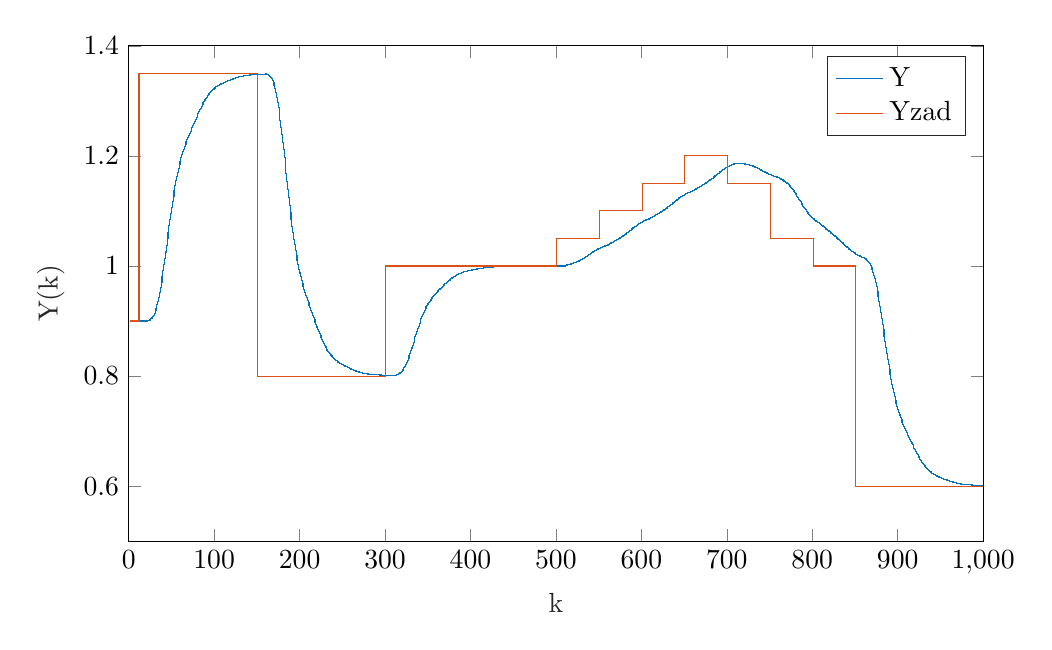
\begin{tikzpicture}

\begin{axis}[%
width=4.272in,
height=2.477in,
at={(0.717in,0.437in)},
scale only axis,
xmin=0,
xmax=1000,
xlabel style={font=\color{white!15!black}},
xlabel={k},
ymin=0.5,
ymax=1.4,
ylabel style={font=\color{white!15!black}},
ylabel={Y(k)},
axis background/.style={fill=white},
legend style={legend cell align=left, align=left, draw=white!15!black}
]
\addplot[const plot, color=mycolor1] table[row sep=crcr] {%
1	0.9\\
2	0.9\\
3	0.9\\
4	0.9\\
5	0.9\\
6	0.9\\
7	0.9\\
8	0.9\\
9	0.9\\
10	0.9\\
11	0.9\\
12	0.9\\
13	0.9\\
14	0.9\\
15	0.9\\
16	0.9\\
17	0.9\\
18	0.9\\
19	0.9\\
20	0.9\\
21	0.9\\
22	0.9003968325\\
23	0.90110505465075\\
24	0.901792976327444\\
25	0.902646481628594\\
26	0.903821675824292\\
27	0.90544848711148\\
28	0.907633879431284\\
29	0.910464715877318\\
30	0.914010308352824\\
31	0.918324685633407\\
32	0.923425663098293\\
33	0.929303840647585\\
34	0.935965438923209\\
35	0.943416013287854\\
36	0.951634745712284\\
37	0.960579528545015\\
38	0.970191311315836\\
39	0.980397805132888\\
40	0.991116627926128\\
41	1.00225796377292\\
42	1.01372812744431\\
43	1.02543354268672\\
44	1.03728153540572\\
45	1.04917966462057\\
46	1.06103743783932\\
47	1.07276903997461\\
48	1.08429539600579\\
49	1.09554568280648\\
50	1.10645838832648\\
51	1.1169820014422\\
52	1.12707532624939\\
53	1.13670736608879\\
54	1.14585695891761\\
55	1.15451243356308\\
56	1.16267122714802\\
57	1.1703392756374\\
58	1.17753016980654\\
59	1.18426415389599\\
60	1.19056702825782\\
61	1.19646900406982\\
62	1.20200355171508\\
63	1.20720628606024\\
64	1.21211392252238\\
65	1.21676331098508\\
66	1.22119054329472\\
67	1.22543014467057\\
68	1.22951436988186\\
69	1.23347262033773\\
70	1.23733099005462\\
71	1.24111194231149\\
72	1.24483411402396\\
73	1.24851224055036\\
74	1.25215718994361\\
75	1.2557760941581\\
76	1.2593725653644\\
77	1.26294698587274\\
78	1.26649685905318\\
79	1.2700172072387\\
80	1.27350100195094\\
81	1.27693961193569\\
82	1.28032325521044\\
83	1.28364144248476\\
84	1.28688340083927\\
85	1.29003846826683\\
86	1.29309645134434\\
87	1.29604793982105\\
88	1.29888457339305\\
89	1.30159925748491\\
90	1.30418632645296\\
91	1.30664165417363\\
92	1.30896271341634\\
93	1.31114858667364\\
94	1.31319993219844\\
95	1.31511890985804\\
96	1.31690907206215\\
97	1.31857522547928\\
98	1.32012326954189\\
99	1.32156001786129\\
100	1.32289300862979\\
101	1.32413030988634\\
102	1.32528032517879\\
103	1.32635160469043\\
104	1.32735266633564\\
105	1.32829183069443\\
106	1.32917707297408\\
107	1.33001589448023\\
108	1.33081521536968\\
109	1.33158128975868\\
110	1.33231964359104\\
111	1.33303503504382\\
112	1.33373143667863\\
113	1.33441203804415\\
114	1.33507926700861\\
115	1.33573482775472\\
116	1.33637975310617\\
117	1.33701446867403\\
118	1.33763886621073\\
119	1.33825238353507\\
120	1.3388540884376\\
121	1.33944276408553\\
122	1.34001699361179\\
123	1.34057524178494\\
124	1.34111593190635\\
125	1.34163751635832\\
126	1.34213853952223\\
127	1.34261769209022\\
128	1.34307385609862\\
129	1.34350614030807\\
130	1.34391390583757\\
131	1.34429678222091\\
132	1.34465467428926\\
133	1.34498776048878\\
134	1.34529648341476\\
135	1.34558153348147\\
136	1.34584382674907\\
137	1.34608447799663\\
138	1.34630477016301\\
139	1.34650612127905\\
140	1.34669004998619\\
141	1.34685814068223\\
142	1.34701200925797\\
143	1.34715327029247\\
144	1.34728350646447\\
145	1.34740424081598\\
146	1.34751691237662\\
147	1.3476228555266\\
148	1.3477232833471\\
149	1.34781927508116\\
150	1.34791176771032\\
151	1.34800155154383\\
152	1.3480892696202\\
153	1.34817542063768\\
154	1.34826036506068\\
155	1.34834433399507\\
156	1.34842744038619\\
157	1.34850969206888\\
158	1.34859100618924\\
159	1.34867122452092\\
160	1.34875012921456\\
161	1.34843062605893\\
162	1.34779790638695\\
163	1.34716201046868\\
164	1.34629858865274\\
165	1.34501935835889\\
166	1.34316774735261\\
167	1.34061500731763\\
168	1.33725674965034\\
169	1.33300986015298\\
170	1.32780975360351\\
171	1.32163087879629\\
172	1.31447733980858\\
173	1.30634095742823\\
174	1.29721934245738\\
175	1.2871417498446\\
176	1.27616294238912\\
177	1.26435794461572\\
178	1.25181757257629\\
179	1.23864463902656\\
180	1.22495074555071\\
181	1.21085225716361\\
182	1.19646593931354\\
183	1.18190777447857\\
184	1.16729311278276\\
185	1.1527343604117\\
186	1.13833773744747\\
187	1.12420083605252\\
188	1.11041083998539\\
189	1.09704328720659\\
190	1.08416127526453\\
191	1.07181510132204\\
192	1.06004237942099\\
193	1.04886844732197\\
194	1.03830679929219\\
195	1.02835961410069\\
196	1.01901856346322\\
197	1.01026589434154\\
198	1.00207569286305\\
199	0.99441525678027\\
200	0.987246519257727\\
201	0.980527475425177\\
202	0.974213563276706\\
203	0.968258961047482\\
204	0.962617790148347\\
205	0.957245223310229\\
206	0.952098482771791\\
207	0.947137703948856\\
208	0.942326646464351\\
209	0.937633244101546\\
210	0.933029992505431\\
211	0.928494179027628\\
212	0.924007963969099\\
213	0.919558326530308\\
214	0.915136890559486\\
215	0.91073964485583\\
216	0.906366572795652\\
217	0.90202120746144\\
218	0.897710129990085\\
219	0.893442429459254\\
220	0.889229142305992\\
221	0.885082688289417\\
222	0.881016318529722\\
223	0.877043589281272\\
224	0.873177873015803\\
225	0.869431916351998\\
226	0.865817452457291\\
227	0.862344873654896\\
228	0.859022968003598\\
229	0.855858721625072\\
230	0.852857186634102\\
231	0.850021412761617\\
232	0.847352439202266\\
233	0.844849341904303\\
234	0.842509330469255\\
235	0.840327888037158\\
236	0.838298946976964\\
237	0.8364150928618\\
238	0.834667789078279\\
239	0.833047614494705\\
240	0.831544506883561\\
241	0.830148005238913\\
242	0.828847484722811\\
243	0.827632378686407\\
244	0.826492383009918\\
245	0.825417638859881\\
246	0.824398890844884\\
247	0.823427618437965\\
248	0.822496139403636\\
249	0.82159768479983\\
250	0.820726445901373\\
251	0.819877594095656\\
252	0.8190472754199\\
253	0.818232581933204\\
254	0.817431502539435\\
255	0.816642856196359\\
256	0.815866210662862\\
257	0.815101790052719\\
258	0.814350374485473\\
259	0.813613195059669\\
260	0.81289182722976\\
261	0.812188085455559\\
262	0.811503921723339\\
263	0.810841330222326\\
264	0.810202260111545\\
265	0.809588537941525\\
266	0.809001800914883\\
267	0.808443441789924\\
268	0.807914565861989\\
269	0.807415960107068\\
270	0.806948074248767\\
271	0.806511013219192\\
272	0.806104540231688\\
273	0.805728089472016\\
274	0.805380787246615\\
275	0.805061480302851\\
276	0.80476876995621\\
277	0.804501050621638\\
278	0.80425655134821\\
279	0.804033378994675\\
280	0.803829561754153\\
281	0.803643091834832\\
282	0.803471966225085\\
283	0.80331422461087\\
284	0.803167983665529\\
285	0.803031467092108\\
286	0.802903030961207\\
287	0.802781184048775\\
288	0.802664603033969\\
289	0.802552142563663\\
290	0.802442840324401\\
291	0.802335917381945\\
292	0.802230774151343\\
293	0.802126982445107\\
294	0.802024274113195\\
295	0.801922526835577\\
296	0.801821747656825\\
297	0.801722054862931\\
298	0.801623658794884\\
299	0.801526842172671\\
300	0.801431940469357\\
301	0.801339322829474\\
302	0.801249373971504\\
303	0.801162477452665\\
304	0.801079000607945\\
305	0.800999281406322\\
306	0.800923617397467\\
307	0.800852256853822\\
308	0.800785392147407\\
309	0.80072315533958\\
310	0.800665615906437\\
311	0.801009432405365\\
312	0.801668802419266\\
313	0.802258407929274\\
314	0.80286868743879\\
315	0.803575929057992\\
316	0.804443966475922\\
317	0.805525694042367\\
318	0.806864419105877\\
319	0.808495067966452\\
320	0.810445260190617\\
321	0.812713329298985\\
322	0.815276397923495\\
323	0.818135464426882\\
324	0.821303566983216\\
325	0.824780441254627\\
326	0.828554991320856\\
327	0.832607407208244\\
328	0.836910973889249\\
329	0.84143361130848\\
330	0.846139180280623\\
331	0.850989911101292\\
332	0.855949432944834\\
333	0.860982601805241\\
334	0.86605354590501\\
335	0.871125901558076\\
336	0.876164268406323\\
337	0.881135331169228\\
338	0.886008704426848\\
339	0.890757548631504\\
340	0.895358998344706\\
341	0.899794360797135\\
342	0.904049000146178\\
343	0.908112074305717\\
344	0.911976408823433\\
345	0.915638471955449\\
346	0.919098255955204\\
347	0.922359021390467\\
348	0.925426944610205\\
349	0.928310700481362\\
350	0.931021005858244\\
351	0.93357014816443\\
352	0.935971529506032\\
353	0.93823925036363\\
354	0.940387730347073\\
355	0.942431350263339\\
356	0.944384113805218\\
357	0.946259340480476\\
358	0.948069400997142\\
359	0.949825501867965\\
360	0.951537522588247\\
361	0.953213905921664\\
362	0.9548615988465\\
363	0.956486038898269\\
364	0.958091179825445\\
365	0.959679551891123\\
366	0.961252353397458\\
367	0.962809569644816\\
368	0.964350114472765\\
369	0.96587198878026\\
370	0.967372450132479\\
371	0.968848187619044\\
372	0.970295496494612\\
373	0.971710447794478\\
374	0.973089048938837\\
375	0.974427392076537\\
376	0.975721787466361\\
377	0.976968879664437\\
378	0.978165744813555\\
379	0.979309967933086\\
380	0.980399699740986\\
381	0.981433693157042\\
382	0.982411320204611\\
383	0.983332570516038\\
384	0.98419803303441\\
385	0.985008862792712\\
386	0.985766734861524\\
387	0.986473787706858\\
388	0.987132558294246\\
389	0.987745911308887\\
390	0.988316964831212\\
391	0.988849014714398\\
392	0.989345459761372\\
393	0.989809729602797\\
394	0.990245216946151\\
395	0.990655215611379\\
396	0.99104286550074\\
397	0.991411105377096\\
398	0.991762634051733\\
399	0.992099880315799\\
400	0.992424981694512\\
401	0.992739771866375\\
402	0.993045776375933\\
403	0.99334421608236\\
404	0.993636017630296\\
405	0.993921830105389\\
406	0.994202046945357\\
407	0.994476832117392\\
408	0.994746149543269\\
409	0.995009794752803\\
410	0.995267427772114\\
411	0.995518606302736\\
412	0.995762818317789\\
413	0.995999513288717\\
414	0.996228131356646\\
415	0.996448129872632\\
416	0.996659006847055\\
417	0.996860320966798\\
418	0.9970517079563\\
419	0.99723289317215\\
420	0.997403700427938\\
421	0.997564057144436\\
422	0.997713996007861\\
423	0.997853653394707\\
424	0.99798326488428\\
425	0.998103158229202\\
426	0.998213744189543\\
427	0.998315505658072\\
428	0.998408985513067\\
429	0.998494773631901\\
430	0.998573493484367\\
431	0.998645788700735\\
432	0.998712309977194\\
433	0.99877370264225\\
434	0.998830595163324\\
435	0.99888358882487\\
436	0.998933248759328\\
437	0.998980096461647\\
438	0.999024603868284\\
439	0.999067189033805\\
440	0.999108213393495\\
441	0.999147980559674\\
442	0.999186736563474\\
443	0.999224671423136\\
444	0.999261921894839\\
445	0.999298575242889\\
446	0.999334673852745\\
447	0.999370220502713\\
448	0.999405184107965\\
449	0.999439505753393\\
450	0.999473104839233\\
451	0.999505885174797\\
452	0.999537740870424\\
453	0.999568561895227\\
454	0.999598239187677\\
455	0.999626669226933\\
456	0.999653757994291\\
457	0.999679424275753\\
458	0.99970360227776\\
459	0.999726243548265\\
460	0.999747318213877\\
461	0.999766815560692\\
462	0.999784744001079\\
463	0.999801130481108\\
464	0.999816019393256\\
465	0.999829471066452\\
466	0.999841559910491\\
467	0.999852372294374\\
468	0.999862004238387\\
469	0.99987055899789\\
470	0.999878144613066\\
471	0.999884871493521\\
472	0.999890850099949\\
473	0.99989618877728\\
474	0.999900991785206\\
475	0.999905357562963\\
476	0.999909377255975\\
477	0.999913133522795\\
478	0.999916699631873\\
479	0.999920138849216\\
480	0.999923504110326\\
481	0.999926837962792\\
482	0.999930172759977\\
483	0.999933531081192\\
484	0.999936926349862\\
485	0.999940363618286\\
486	0.999943840485815\\
487	0.999947348116464\\
488	0.999950872322155\\
489	0.999954394678819\\
490	0.999957893644386\\
491	0.999961345650168\\
492	0.999964726140156\\
493	0.999968010536166\\
494	0.999971175110496\\
495	0.999974197751661\\
496	0.999977058612702\\
497	0.999979740635494\\
498	0.999982229948198\\
499	0.999984516136535\\
500	0.999986592392781\\
501	0.999988455549186\\
502	0.999990106005001\\
503	0.999991547558265\\
504	0.999992787155045\\
505	0.999993834569912\\
506	0.999994702032071\\
507	0.999995403811769\\
508	0.999995955781397\\
509	0.999996374965183\\
510	0.99999667909049\\
511	1.00039371700121\\
512	1.00110205978487\\
513	1.00170452890047\\
514	1.00223442784612\\
515	1.00272038028179\\
516	1.00318686955165\\
517	1.0036547213546\\
518	1.00414153526502\\
519	1.0046620702517\\
520	1.00522858884009\\
521	1.00582821847735\\
522	1.00643043429556\\
523	1.00703349693446\\
524	1.00765531343145\\
525	1.00830831897024\\
526	1.00900037010485\\
527	1.00973551670104\\
528	1.0105146676046\\
529	1.0113361632921\\
530	1.0121962672022\\
531	1.01309091283139\\
532	1.01401816767096\\
533	1.01497748771482\\
534	1.01596699536437\\
535	1.01698282948864\\
536	1.01801983858944\\
537	1.01907214104967\\
538	1.02013357339064\\
539	1.02119804450322\\
540	1.02225981124717\\
541	1.02331361186821\\
542	1.02435455430727\\
543	1.02537791714391\\
544	1.02637915665831\\
545	1.02735409872487\\
546	1.02829911650706\\
547	1.0292112294243\\
548	1.03008814115479\\
549	1.03092823124144\\
550	1.03173051217918\\
551	1.03249456604228\\
552	1.03322048342288\\
553	1.03390882289695\\
554	1.0345605828393\\
555	1.0351771630118\\
556	1.03576030705612\\
557	1.03631203200471\\
558	1.03683455310695\\
559	1.03733021005661\\
560	1.03780139894673\\
561	1.03864646009087\\
562	1.03978062933444\\
563	1.04078845569021\\
564	1.04170584153618\\
565	1.04256377732673\\
566	1.04338885994869\\
567	1.04420376095814\\
568	1.04502765111153\\
569	1.04587658622872\\
570	1.04676385836263\\
571	1.04767742089744\\
572	1.04858747919757\\
573	1.04949291812835\\
574	1.05041206033849\\
575	1.05135752372197\\
576	1.05233715226248\\
577	1.05335482517619\\
578	1.05441115872375\\
579	1.05550411329506\\
580	1.05662951687788\\
581	1.05778283856339\\
582	1.05896166786602\\
583	1.06016497857712\\
584	1.06139042209532\\
585	1.06263369927022\\
586	1.06388927360866\\
587	1.06515094659502\\
588	1.06641231640585\\
589	1.06766713837913\\
590	1.06890960306704\\
591	1.07013446895497\\
592	1.07133694801071\\
593	1.07251250283952\\
594	1.07365684893903\\
595	1.07476614009545\\
596	1.07583713770013\\
597	1.07686729990107\\
598	1.0778548089296\\
599	1.07879855167543\\
600	1.07969806582385\\
601	1.08055346597064\\
602	1.08136537272994\\
603	1.0821348631683\\
604	1.08286343444368\\
605	1.08355295816932\\
606	1.08420561677659\\
607	1.08482382811431\\
608	1.08541016664575\\
609	1.08596728733359\\
610	1.08649785649315\\
611	1.08740029874762\\
612	1.08858979157341\\
613	1.08965096349308\\
614	1.09061989152446\\
615	1.09152769606599\\
616	1.0924010642635\\
617	1.09326272354918\\
618	1.09413187163108\\
619	1.09502456783777\\
620	1.09595408966757\\
621	1.09690837119914\\
622	1.09785761164597\\
623	1.09880070141734\\
624	1.09975596619931\\
625	1.10073602132407\\
626	1.10174870703268\\
627	1.10279790126932\\
628	1.10388422439776\\
629	1.10500564847573\\
630	1.10615802224048\\
631	1.1073368450397\\
632	1.10853974483626\\
633	1.10976573995174\\
634	1.11101253131745\\
635	1.11227587427123\\
636	1.11355029165787\\
637	1.1148296486198\\
638	1.11610761046075\\
639	1.11737800203711\\
640	1.11863508459076\\
641	1.11987368720899\\
642	1.12108909123382\\
643	1.12227682652874\\
644	1.12343267306638\\
645	1.12455284575047\\
646	1.12563416319222\\
647	1.12667413638053\\
648	1.12767099562436\\
649	1.12862367086563\\
650	1.12953173769107\\
651	1.130395343462\\
652	1.13121513656646\\
653	1.13199221710025\\
654	1.13272810082519\\
655	1.13342467390489\\
656	1.13408412968347\\
657	1.13470889373864\\
658	1.1353015455611\\
659	1.13586474293777\\
660	1.13640115330537\\
661	1.13730920133227\\
662	1.13850406499274\\
663	1.1395703725617\\
664	1.14054419953204\\
665	1.14145666520854\\
666	1.14233445634978\\
667	1.14320030092966\\
668	1.14407339829573\\
669	1.14496981062909\\
670	1.14590281955634\\
671	1.1468603645655\\
672	1.14781265145131\\
673	1.14875857826562\\
674	1.14971647939645\\
675	1.15069897987251\\
676	1.15171393046093\\
677	1.15276522028194\\
678	1.15385348133693\\
679	1.15497669759129\\
680	1.1561307297708\\
681	1.15731108911111\\
682	1.15851541519744\\
683	1.15974273756478\\
684	1.16099076781911\\
685	1.16225527131521\\
686	1.16353078015669\\
687	1.16481116791043\\
688	1.16609010741786\\
689	1.16736143015747\\
690	1.16861940307084\\
691	1.1698588600365\\
692	1.17107508631148\\
693	1.17226361484566\\
694	1.17342022792995\\
695	1.17454114208971\\
696	1.17562317694168\\
697	1.17666384395119\\
698	1.17766137346496\\
699	1.17861469511554\\
700	1.17952338392319\\
701	1.18038758651215\\
702	1.18120795044366\\
703	1.18198557497114\\
704	1.18272197506439\\
705	1.1834190362023\\
706	1.184078951199\\
707	1.18470414529443\\
708	1.18529719786099\\
709	1.18586076680438\\
710	1.18639751992523\\
711	1.18651221831475\\
712	1.18629092785924\\
713	1.18615266683395\\
714	1.18606693990674\\
715	1.18600765286384\\
716	1.18595255672064\\
717	1.18588275575563\\
718	1.18578227434336\\
719	1.18563767719582\\
720	1.18543773756889\\
721	1.18519615310595\\
722	1.18494418921743\\
723	1.1846842295491\\
724	1.18439879803255\\
725	1.18407564975217\\
726	1.18370691998225\\
727	1.18328839333299\\
728	1.18281887737155\\
729	1.18229966683755\\
730	1.18173408620468\\
731	1.18112576964288\\
732	1.18047621133567\\
733	1.17978551836803\\
734	1.17905514733567\\
735	1.17828857620041\\
736	1.17749063122264\\
737	1.17666694138931\\
738	1.17582349986878\\
739	1.17496631501848\\
740	1.17410113607155\\
741	1.1732333177918\\
742	1.17236792827358\\
743	1.17150994331535\\
744	1.17066423386293\\
745	1.16983536700897\\
746	1.16902741933029\\
747	1.16824386756392\\
748	1.16748753947557\\
749	1.16676061088764\\
750	1.16606463744184\\
751	1.16540060740034\\
752	1.16476899294972\\
753	1.16416978188346\\
754	1.16360249786905\\
755	1.16306623195307\\
756	1.16255969430794\\
757	1.16208128022535\\
758	1.16162914211492\\
759	1.16120126141339\\
760	1.16079551601878\\
761	1.16001365145738\\
762	1.15894037457367\\
763	1.15798052877069\\
764	1.15707931156364\\
765	1.15618992529156\\
766	1.15527268133295\\
767	1.15429419618655\\
768	1.1532266686384\\
769	1.15204722902929\\
770	1.15073735308466\\
771	1.1493052366589\\
772	1.14777803356319\\
773	1.14615587666895\\
774	1.14442199873985\\
775	1.14256794553579\\
776	1.14059212541136\\
777	1.13849855678803\\
778	1.1362957892123\\
779	1.13399597668459\\
780	1.13161408450484\\
781	1.12916588880959\\
782	1.12666530645259\\
783	1.12412493653425\\
784	1.12155850920695\\
785	1.11898121798116\\
786	1.11640875182568\\
787	1.11385653142127\\
788	1.11133911657954\\
789	1.10886975653239\\
790	1.10646005885781\\
791	1.10411983289513\\
792	1.10185720361568\\
793	1.09967883431872\\
794	1.09758996761927\\
795	1.09559431135825\\
796	1.09369396722249\\
797	1.0918894590782\\
798	1.09017983527501\\
799	1.08856282402788\\
800	1.08703502504983\\
801	1.08559211957906\\
802	1.08422907321397\\
803	1.08294031123552\\
804	1.08171987260122\\
805	1.08056156278147\\
806	1.07945911175469\\
807	1.0784063290746\\
808	1.07739724665759\\
809	1.07642624295296\\
810	1.07548814451595\\
811	1.07418433515173\\
812	1.07260125407848\\
813	1.07115400700819\\
814	1.06980490870859\\
815	1.06852177024251\\
816	1.06727732297586\\
817	1.06604868700549\\
818	1.06481687942964\\
819	1.06356635924957\\
820	1.06228460667134\\
821	1.06098451533583\\
822	1.05969655059005\\
823	1.05842234209261\\
824	1.05714412786465\\
825	1.05584994110756\\
826	1.05453261466811\\
827	1.05318891719762\\
828	1.05181880653853\\
829	1.05042478747156\\
830	1.04901136229311\\
831	1.04758324662967\\
832	1.04614290411372\\
833	1.04469130814368\\
834	1.04323065994807\\
835	1.04176501379597\\
836	1.04029956211728\\
837	1.03884006510026\\
838	1.03739240207448\\
839	1.03596222500649\\
840	1.03455469707677\\
841	1.03317437778697\\
842	1.03182535416059\\
843	1.0305114573318\\
844	1.02923627138778\\
845	1.02800295817699\\
846	1.02681409807654\\
847	1.02567161037729\\
848	1.02457673432857\\
849	1.02353005532998\\
850	1.02253156367392\\
851	1.02158073130043\\
852	1.02067658363713\\
853	1.01981774850737\\
854	1.01900249060918\\
855	1.01822875428551\\
856	1.01749422339825\\
857	1.01679639213189\\
858	1.01613263848402\\
859	1.01550029452341\\
860	1.0148967093382\\
861	1.01392353205634\\
862	1.01266568549135\\
863	1.01146379194913\\
864	1.01014830344722\\
865	1.00857659232235\\
866	1.00662974385191\\
867	1.00420968986861\\
868	1.00123664753952\\
869	0.997646831740664\\
870	0.993390413119296\\
871	0.988452581380834\\
872	0.982844607621753\\
873	0.9765605717512\\
874	0.969592876250273\\
875	0.961957909878341\\
876	0.953691446749461\\
877	0.944844706977621\\
878	0.935480994812871\\
879	0.925672840303994\\
880	0.915499579409624\\
881	0.90504399207581\\
882	0.894388501716754\\
883	0.883614569599948\\
884	0.872803608165325\\
885	0.862035541126998\\
886	0.851386310405085\\
887	0.840925987841813\\
888	0.83071738761177\\
889	0.820815090658765\\
890	0.811264805808438\\
891	0.802103080205753\\
892	0.793357418552412\\
893	0.785046631350171\\
894	0.777181139683411\\
895	0.769763292308008\\
896	0.762787884762076\\
897	0.756242894860035\\
898	0.750110364153481\\
899	0.744367369391171\\
900	0.738987040002324\\
901	0.733939583114274\\
902	0.729193275221195\\
903	0.724715388508976\\
904	0.720473046675956\\
905	0.716434016746523\\
906	0.712567428819872\\
907	0.708844404630999\\
908	0.705238579707156\\
909	0.701726511398523\\
910	0.698287970715558\\
911	0.694906120329759\\
912	0.691567585169746\\
913	0.68826242557543\\
914	0.684984024338255\\
915	0.681728898155307\\
916	0.678496443502662\\
917	0.675288627904062\\
918	0.672109638909076\\
919	0.66896550375867\\
920	0.665863692647641\\
921	0.662812717896865\\
922	0.659821740332846\\
923	0.65690019280369\\
924	0.654057429206078\\
925	0.651302405904297\\
926	0.648643401084628\\
927	0.646087776293423\\
928	0.643641783046377\\
929	0.641310415988031\\
930	0.639097312702113\\
931	0.63700469899082\\
932	0.635033377299871\\
933	0.633182755000572\\
934	0.631450908469906\\
935	0.629834678331045\\
936	0.628329790807601\\
937	0.626930999886161\\
938	0.625632244867703\\
939	0.624426817919554\\
940	0.623307536410482\\
941	0.622266915109787\\
942	0.621297333739002\\
943	0.62039119586067\\
944	0.619541075649477\\
945	0.618739849693879\\
946	0.617980811601001\\
947	0.617257767806917\\
948	0.616565113613426\\
949	0.615897889067111\\
950	0.615251814853368\\
951	0.614623308885504\\
952	0.614009484717019\\
953	0.613408133286624\\
954	0.612817689815588\\
955	0.612237187913612\\
956	0.611666203112794\\
957	0.611104788141406\\
958	0.610553402273809\\
959	0.610012837054638\\
960	0.609484140600628\\
961	0.6089685425389\\
962	0.608467381454282\\
963	0.607982036498353\\
964	0.607513864568163\\
965	0.607064144201329\\
966	0.606634027064722\\
967	0.606224497643939\\
968	0.605836341477269\\
969	0.605470122027138\\
970	0.605126166049681\\
971	0.604804557113496\\
972	0.604505136735531\\
973	0.604227512447966\\
974	0.603971071986485\\
975	0.603735002698274\\
976	0.60351831520709\\
977	0.603319870341987\\
978	0.603138408333929\\
979	0.602972579308368\\
980	0.602820974149068\\
981	0.602682154875911\\
982	0.602554683763622\\
983	0.602437150525799\\
984	0.602328196995612\\
985	0.602226538847511\\
986	0.602130984019804\\
987	0.602040447612789\\
988	0.601953963148308\\
989	0.601870690181603\\
990	0.601789918352816\\
991	0.601711068051767\\
992	0.601633687944194\\
993	0.601557449669557\\
994	0.601482140069199\\
995	0.601407651338948\\
996	0.601333969522305\\
997	0.601261161769759\\
998	0.601189362787216\\
999	0.601118760883205\\
1000	0.601049584001516\\
};
\addlegendentry{Y}

\addplot[const plot, color=mycolor2] table[row sep=crcr] {%
1	0.9\\
2	0.9\\
3	0.9\\
4	0.9\\
5	0.9\\
6	0.9\\
7	0.9\\
8	0.9\\
9	0.9\\
10	0.9\\
11	0.9\\
12	1.35\\
13	1.35\\
14	1.35\\
15	1.35\\
16	1.35\\
17	1.35\\
18	1.35\\
19	1.35\\
20	1.35\\
21	1.35\\
22	1.35\\
23	1.35\\
24	1.35\\
25	1.35\\
26	1.35\\
27	1.35\\
28	1.35\\
29	1.35\\
30	1.35\\
31	1.35\\
32	1.35\\
33	1.35\\
34	1.35\\
35	1.35\\
36	1.35\\
37	1.35\\
38	1.35\\
39	1.35\\
40	1.35\\
41	1.35\\
42	1.35\\
43	1.35\\
44	1.35\\
45	1.35\\
46	1.35\\
47	1.35\\
48	1.35\\
49	1.35\\
50	1.35\\
51	1.35\\
52	1.35\\
53	1.35\\
54	1.35\\
55	1.35\\
56	1.35\\
57	1.35\\
58	1.35\\
59	1.35\\
60	1.35\\
61	1.35\\
62	1.35\\
63	1.35\\
64	1.35\\
65	1.35\\
66	1.35\\
67	1.35\\
68	1.35\\
69	1.35\\
70	1.35\\
71	1.35\\
72	1.35\\
73	1.35\\
74	1.35\\
75	1.35\\
76	1.35\\
77	1.35\\
78	1.35\\
79	1.35\\
80	1.35\\
81	1.35\\
82	1.35\\
83	1.35\\
84	1.35\\
85	1.35\\
86	1.35\\
87	1.35\\
88	1.35\\
89	1.35\\
90	1.35\\
91	1.35\\
92	1.35\\
93	1.35\\
94	1.35\\
95	1.35\\
96	1.35\\
97	1.35\\
98	1.35\\
99	1.35\\
100	1.35\\
101	1.35\\
102	1.35\\
103	1.35\\
104	1.35\\
105	1.35\\
106	1.35\\
107	1.35\\
108	1.35\\
109	1.35\\
110	1.35\\
111	1.35\\
112	1.35\\
113	1.35\\
114	1.35\\
115	1.35\\
116	1.35\\
117	1.35\\
118	1.35\\
119	1.35\\
120	1.35\\
121	1.35\\
122	1.35\\
123	1.35\\
124	1.35\\
125	1.35\\
126	1.35\\
127	1.35\\
128	1.35\\
129	1.35\\
130	1.35\\
131	1.35\\
132	1.35\\
133	1.35\\
134	1.35\\
135	1.35\\
136	1.35\\
137	1.35\\
138	1.35\\
139	1.35\\
140	1.35\\
141	1.35\\
142	1.35\\
143	1.35\\
144	1.35\\
145	1.35\\
146	1.35\\
147	1.35\\
148	1.35\\
149	1.35\\
150	1.35\\
151	0.8\\
152	0.8\\
153	0.8\\
154	0.8\\
155	0.8\\
156	0.8\\
157	0.8\\
158	0.8\\
159	0.8\\
160	0.8\\
161	0.8\\
162	0.8\\
163	0.8\\
164	0.8\\
165	0.8\\
166	0.8\\
167	0.8\\
168	0.8\\
169	0.8\\
170	0.8\\
171	0.8\\
172	0.8\\
173	0.8\\
174	0.8\\
175	0.8\\
176	0.8\\
177	0.8\\
178	0.8\\
179	0.8\\
180	0.8\\
181	0.8\\
182	0.8\\
183	0.8\\
184	0.8\\
185	0.8\\
186	0.8\\
187	0.8\\
188	0.8\\
189	0.8\\
190	0.8\\
191	0.8\\
192	0.8\\
193	0.8\\
194	0.8\\
195	0.8\\
196	0.8\\
197	0.8\\
198	0.8\\
199	0.8\\
200	0.8\\
201	0.8\\
202	0.8\\
203	0.8\\
204	0.8\\
205	0.8\\
206	0.8\\
207	0.8\\
208	0.8\\
209	0.8\\
210	0.8\\
211	0.8\\
212	0.8\\
213	0.8\\
214	0.8\\
215	0.8\\
216	0.8\\
217	0.8\\
218	0.8\\
219	0.8\\
220	0.8\\
221	0.8\\
222	0.8\\
223	0.8\\
224	0.8\\
225	0.8\\
226	0.8\\
227	0.8\\
228	0.8\\
229	0.8\\
230	0.8\\
231	0.8\\
232	0.8\\
233	0.8\\
234	0.8\\
235	0.8\\
236	0.8\\
237	0.8\\
238	0.8\\
239	0.8\\
240	0.8\\
241	0.8\\
242	0.8\\
243	0.8\\
244	0.8\\
245	0.8\\
246	0.8\\
247	0.8\\
248	0.8\\
249	0.8\\
250	0.8\\
251	0.8\\
252	0.8\\
253	0.8\\
254	0.8\\
255	0.8\\
256	0.8\\
257	0.8\\
258	0.8\\
259	0.8\\
260	0.8\\
261	0.8\\
262	0.8\\
263	0.8\\
264	0.8\\
265	0.8\\
266	0.8\\
267	0.8\\
268	0.8\\
269	0.8\\
270	0.8\\
271	0.8\\
272	0.8\\
273	0.8\\
274	0.8\\
275	0.8\\
276	0.8\\
277	0.8\\
278	0.8\\
279	0.8\\
280	0.8\\
281	0.8\\
282	0.8\\
283	0.8\\
284	0.8\\
285	0.8\\
286	0.8\\
287	0.8\\
288	0.8\\
289	0.8\\
290	0.8\\
291	0.8\\
292	0.8\\
293	0.8\\
294	0.8\\
295	0.8\\
296	0.8\\
297	0.8\\
298	0.8\\
299	0.8\\
300	0.8\\
301	1\\
302	1\\
303	1\\
304	1\\
305	1\\
306	1\\
307	1\\
308	1\\
309	1\\
310	1\\
311	1\\
312	1\\
313	1\\
314	1\\
315	1\\
316	1\\
317	1\\
318	1\\
319	1\\
320	1\\
321	1\\
322	1\\
323	1\\
324	1\\
325	1\\
326	1\\
327	1\\
328	1\\
329	1\\
330	1\\
331	1\\
332	1\\
333	1\\
334	1\\
335	1\\
336	1\\
337	1\\
338	1\\
339	1\\
340	1\\
341	1\\
342	1\\
343	1\\
344	1\\
345	1\\
346	1\\
347	1\\
348	1\\
349	1\\
350	1\\
351	1\\
352	1\\
353	1\\
354	1\\
355	1\\
356	1\\
357	1\\
358	1\\
359	1\\
360	1\\
361	1\\
362	1\\
363	1\\
364	1\\
365	1\\
366	1\\
367	1\\
368	1\\
369	1\\
370	1\\
371	1\\
372	1\\
373	1\\
374	1\\
375	1\\
376	1\\
377	1\\
378	1\\
379	1\\
380	1\\
381	1\\
382	1\\
383	1\\
384	1\\
385	1\\
386	1\\
387	1\\
388	1\\
389	1\\
390	1\\
391	1\\
392	1\\
393	1\\
394	1\\
395	1\\
396	1\\
397	1\\
398	1\\
399	1\\
400	1\\
401	1\\
402	1\\
403	1\\
404	1\\
405	1\\
406	1\\
407	1\\
408	1\\
409	1\\
410	1\\
411	1\\
412	1\\
413	1\\
414	1\\
415	1\\
416	1\\
417	1\\
418	1\\
419	1\\
420	1\\
421	1\\
422	1\\
423	1\\
424	1\\
425	1\\
426	1\\
427	1\\
428	1\\
429	1\\
430	1\\
431	1\\
432	1\\
433	1\\
434	1\\
435	1\\
436	1\\
437	1\\
438	1\\
439	1\\
440	1\\
441	1\\
442	1\\
443	1\\
444	1\\
445	1\\
446	1\\
447	1\\
448	1\\
449	1\\
450	1\\
451	1\\
452	1\\
453	1\\
454	1\\
455	1\\
456	1\\
457	1\\
458	1\\
459	1\\
460	1\\
461	1\\
462	1\\
463	1\\
464	1\\
465	1\\
466	1\\
467	1\\
468	1\\
469	1\\
470	1\\
471	1\\
472	1\\
473	1\\
474	1\\
475	1\\
476	1\\
477	1\\
478	1\\
479	1\\
480	1\\
481	1\\
482	1\\
483	1\\
484	1\\
485	1\\
486	1\\
487	1\\
488	1\\
489	1\\
490	1\\
491	1\\
492	1\\
493	1\\
494	1\\
495	1\\
496	1\\
497	1\\
498	1\\
499	1\\
500	1\\
501	1.05\\
502	1.05\\
503	1.05\\
504	1.05\\
505	1.05\\
506	1.05\\
507	1.05\\
508	1.05\\
509	1.05\\
510	1.05\\
511	1.05\\
512	1.05\\
513	1.05\\
514	1.05\\
515	1.05\\
516	1.05\\
517	1.05\\
518	1.05\\
519	1.05\\
520	1.05\\
521	1.05\\
522	1.05\\
523	1.05\\
524	1.05\\
525	1.05\\
526	1.05\\
527	1.05\\
528	1.05\\
529	1.05\\
530	1.05\\
531	1.05\\
532	1.05\\
533	1.05\\
534	1.05\\
535	1.05\\
536	1.05\\
537	1.05\\
538	1.05\\
539	1.05\\
540	1.05\\
541	1.05\\
542	1.05\\
543	1.05\\
544	1.05\\
545	1.05\\
546	1.05\\
547	1.05\\
548	1.05\\
549	1.05\\
550	1.05\\
551	1.1\\
552	1.1\\
553	1.1\\
554	1.1\\
555	1.1\\
556	1.1\\
557	1.1\\
558	1.1\\
559	1.1\\
560	1.1\\
561	1.1\\
562	1.1\\
563	1.1\\
564	1.1\\
565	1.1\\
566	1.1\\
567	1.1\\
568	1.1\\
569	1.1\\
570	1.1\\
571	1.1\\
572	1.1\\
573	1.1\\
574	1.1\\
575	1.1\\
576	1.1\\
577	1.1\\
578	1.1\\
579	1.1\\
580	1.1\\
581	1.1\\
582	1.1\\
583	1.1\\
584	1.1\\
585	1.1\\
586	1.1\\
587	1.1\\
588	1.1\\
589	1.1\\
590	1.1\\
591	1.1\\
592	1.1\\
593	1.1\\
594	1.1\\
595	1.1\\
596	1.1\\
597	1.1\\
598	1.1\\
599	1.1\\
600	1.1\\
601	1.15\\
602	1.15\\
603	1.15\\
604	1.15\\
605	1.15\\
606	1.15\\
607	1.15\\
608	1.15\\
609	1.15\\
610	1.15\\
611	1.15\\
612	1.15\\
613	1.15\\
614	1.15\\
615	1.15\\
616	1.15\\
617	1.15\\
618	1.15\\
619	1.15\\
620	1.15\\
621	1.15\\
622	1.15\\
623	1.15\\
624	1.15\\
625	1.15\\
626	1.15\\
627	1.15\\
628	1.15\\
629	1.15\\
630	1.15\\
631	1.15\\
632	1.15\\
633	1.15\\
634	1.15\\
635	1.15\\
636	1.15\\
637	1.15\\
638	1.15\\
639	1.15\\
640	1.15\\
641	1.15\\
642	1.15\\
643	1.15\\
644	1.15\\
645	1.15\\
646	1.15\\
647	1.15\\
648	1.15\\
649	1.15\\
650	1.15\\
651	1.2\\
652	1.2\\
653	1.2\\
654	1.2\\
655	1.2\\
656	1.2\\
657	1.2\\
658	1.2\\
659	1.2\\
660	1.2\\
661	1.2\\
662	1.2\\
663	1.2\\
664	1.2\\
665	1.2\\
666	1.2\\
667	1.2\\
668	1.2\\
669	1.2\\
670	1.2\\
671	1.2\\
672	1.2\\
673	1.2\\
674	1.2\\
675	1.2\\
676	1.2\\
677	1.2\\
678	1.2\\
679	1.2\\
680	1.2\\
681	1.2\\
682	1.2\\
683	1.2\\
684	1.2\\
685	1.2\\
686	1.2\\
687	1.2\\
688	1.2\\
689	1.2\\
690	1.2\\
691	1.2\\
692	1.2\\
693	1.2\\
694	1.2\\
695	1.2\\
696	1.2\\
697	1.2\\
698	1.2\\
699	1.2\\
700	1.2\\
701	1.15\\
702	1.15\\
703	1.15\\
704	1.15\\
705	1.15\\
706	1.15\\
707	1.15\\
708	1.15\\
709	1.15\\
710	1.15\\
711	1.15\\
712	1.15\\
713	1.15\\
714	1.15\\
715	1.15\\
716	1.15\\
717	1.15\\
718	1.15\\
719	1.15\\
720	1.15\\
721	1.15\\
722	1.15\\
723	1.15\\
724	1.15\\
725	1.15\\
726	1.15\\
727	1.15\\
728	1.15\\
729	1.15\\
730	1.15\\
731	1.15\\
732	1.15\\
733	1.15\\
734	1.15\\
735	1.15\\
736	1.15\\
737	1.15\\
738	1.15\\
739	1.15\\
740	1.15\\
741	1.15\\
742	1.15\\
743	1.15\\
744	1.15\\
745	1.15\\
746	1.15\\
747	1.15\\
748	1.15\\
749	1.15\\
750	1.15\\
751	1.05\\
752	1.05\\
753	1.05\\
754	1.05\\
755	1.05\\
756	1.05\\
757	1.05\\
758	1.05\\
759	1.05\\
760	1.05\\
761	1.05\\
762	1.05\\
763	1.05\\
764	1.05\\
765	1.05\\
766	1.05\\
767	1.05\\
768	1.05\\
769	1.05\\
770	1.05\\
771	1.05\\
772	1.05\\
773	1.05\\
774	1.05\\
775	1.05\\
776	1.05\\
777	1.05\\
778	1.05\\
779	1.05\\
780	1.05\\
781	1.05\\
782	1.05\\
783	1.05\\
784	1.05\\
785	1.05\\
786	1.05\\
787	1.05\\
788	1.05\\
789	1.05\\
790	1.05\\
791	1.05\\
792	1.05\\
793	1.05\\
794	1.05\\
795	1.05\\
796	1.05\\
797	1.05\\
798	1.05\\
799	1.05\\
800	1.05\\
801	1\\
802	1\\
803	1\\
804	1\\
805	1\\
806	1\\
807	1\\
808	1\\
809	1\\
810	1\\
811	1\\
812	1\\
813	1\\
814	1\\
815	1\\
816	1\\
817	1\\
818	1\\
819	1\\
820	1\\
821	1\\
822	1\\
823	1\\
824	1\\
825	1\\
826	1\\
827	1\\
828	1\\
829	1\\
830	1\\
831	1\\
832	1\\
833	1\\
834	1\\
835	1\\
836	1\\
837	1\\
838	1\\
839	1\\
840	1\\
841	1\\
842	1\\
843	1\\
844	1\\
845	1\\
846	1\\
847	1\\
848	1\\
849	1\\
850	1\\
851	0.6\\
852	0.6\\
853	0.6\\
854	0.6\\
855	0.6\\
856	0.6\\
857	0.6\\
858	0.6\\
859	0.6\\
860	0.6\\
861	0.6\\
862	0.6\\
863	0.6\\
864	0.6\\
865	0.6\\
866	0.6\\
867	0.6\\
868	0.6\\
869	0.6\\
870	0.6\\
871	0.6\\
872	0.6\\
873	0.6\\
874	0.6\\
875	0.6\\
876	0.6\\
877	0.6\\
878	0.6\\
879	0.6\\
880	0.6\\
881	0.6\\
882	0.6\\
883	0.6\\
884	0.6\\
885	0.6\\
886	0.6\\
887	0.6\\
888	0.6\\
889	0.6\\
890	0.6\\
891	0.6\\
892	0.6\\
893	0.6\\
894	0.6\\
895	0.6\\
896	0.6\\
897	0.6\\
898	0.6\\
899	0.6\\
900	0.6\\
901	0.6\\
902	0.6\\
903	0.6\\
904	0.6\\
905	0.6\\
906	0.6\\
907	0.6\\
908	0.6\\
909	0.6\\
910	0.6\\
911	0.6\\
912	0.6\\
913	0.6\\
914	0.6\\
915	0.6\\
916	0.6\\
917	0.6\\
918	0.6\\
919	0.6\\
920	0.6\\
921	0.6\\
922	0.6\\
923	0.6\\
924	0.6\\
925	0.6\\
926	0.6\\
927	0.6\\
928	0.6\\
929	0.6\\
930	0.6\\
931	0.6\\
932	0.6\\
933	0.6\\
934	0.6\\
935	0.6\\
936	0.6\\
937	0.6\\
938	0.6\\
939	0.6\\
940	0.6\\
941	0.6\\
942	0.6\\
943	0.6\\
944	0.6\\
945	0.6\\
946	0.6\\
947	0.6\\
948	0.6\\
949	0.6\\
950	0.6\\
951	0.6\\
952	0.6\\
953	0.6\\
954	0.6\\
955	0.6\\
956	0.6\\
957	0.6\\
958	0.6\\
959	0.6\\
960	0.6\\
961	0.6\\
962	0.6\\
963	0.6\\
964	0.6\\
965	0.6\\
966	0.6\\
967	0.6\\
968	0.6\\
969	0.6\\
970	0.6\\
971	0.6\\
972	0.6\\
973	0.6\\
974	0.6\\
975	0.6\\
976	0.6\\
977	0.6\\
978	0.6\\
979	0.6\\
980	0.6\\
981	0.6\\
982	0.6\\
983	0.6\\
984	0.6\\
985	0.6\\
986	0.6\\
987	0.6\\
988	0.6\\
989	0.6\\
990	0.6\\
991	0.6\\
992	0.6\\
993	0.6\\
994	0.6\\
995	0.6\\
996	0.6\\
997	0.6\\
998	0.6\\
999	0.6\\
1000	0.6\\
};
\addlegendentry{Yzad}

\end{axis}
\end{tikzpicture}%
\caption{Śledzenie wartości zadanej dla parametrów $K = 1,212$, $T_i = 15$, $T_d = 4$}
\end{figure}

Wskaźnik jakości regulacji:

\begin{equation}
E = 25,6710
\end{equation}

Wartości parametrów dla których wartość wyjścia najlepiej śledzi wartość zadaną (na oko) to:

\begin{equation}
K = 1,3; T_i = 10; T_d = 3;
\end{equation}

\begin{figure}[H]
\centering
% This file was created by matlab2tikz.
%
%The latest updates can be retrieved from
%  http://www.mathworks.com/matlabcentral/fileexchange/22022-matlab2tikz-matlab2tikz
%where you can also make suggestions and rate matlab2tikz.
%
\definecolor{mycolor1}{rgb}{0.00000,0.44700,0.74100}%
%
\begin{tikzpicture}

\begin{axis}[%
width=4.272in,
height=2.477in,
at={(0.717in,0.437in)},
scale only axis,
xmin=0,
xmax=1000,
xlabel style={font=\color{white!15!black}},
xlabel={k},
ymin=2.7,
ymax=3.3,
ylabel style={font=\color{white!15!black}},
ylabel={U(k)},
axis background/.style={fill=white}
]
\addplot[const plot, color=mycolor1, forget plot] table[row sep=crcr] {%
1	3\\
2	3\\
3	3\\
4	3\\
5	3\\
6	3\\
7	3\\
8	3\\
9	3\\
10	3\\
11	3\\
12	3.075\\
13	3\\
14	3.02925\\
15	3.0585\\
16	3.08775\\
17	3.117\\
18	3.14625\\
19	3.1755\\
20	3.20475\\
21	3.234\\
22	3.25962592719375\\
23	3.28547758778953\\
24	3.3\\
25	3.3\\
26	3.3\\
27	3.3\\
28	3.3\\
29	3.3\\
30	3.3\\
31	3.3\\
32	3.3\\
33	3.3\\
34	3.3\\
35	3.3\\
36	3.3\\
37	3.3\\
38	3.3\\
39	3.3\\
40	3.3\\
41	3.3\\
42	3.3\\
43	3.3\\
44	3.3\\
45	3.3\\
46	3.3\\
47	3.3\\
48	3.3\\
49	3.3\\
50	3.3\\
51	3.3\\
52	3.3\\
53	3.29999906788716\\
54	3.29989615394184\\
55	3.29969413415641\\
56	3.29939607445979\\
57	3.29900518175031\\
58	3.29852476159182\\
59	3.29795818181419\\
60	3.29730884133915\\
61	3.29658014362351\\
62	3.2957754741763\\
63	3.29489822670512\\
64	3.2939566673918\\
65	3.29296343597744\\
66	3.29193075207795\\
67	3.29087041086821\\
68	3.28979378207084\\
69	3.28871181170071\\
70	3.28763502609109\\
71	3.28657353779293\\
72	3.28553705299544\\
73	3.28453487799008\\
74	3.28357568874757\\
75	3.28266710362615\\
76	3.28181551294273\\
77	3.28102612746637\\
78	3.28030302497752\\
79	3.27964919493\\
80	3.27906658126531\\
81	3.27855612343809\\
82	3.27811779571788\\
83	3.27775064494117\\
84	3.27745283837678\\
85	3.27722174210043\\
86	3.27705402636426\\
87	3.27694577561768\\
88	3.27689259344666\\
89	3.27688970284671\\
90	3.27693204220213\\
91	3.27701435730552\\
92	3.27713128971614\\
93	3.27727746171895\\
94	3.27744755755259\\
95	3.27763639904149\\
96	3.2778390130042\\
97	3.27805068905315\\
98	3.2782670278833\\
99	3.27848398055016\\
100	3.27869787917931\\
101	3.27890545949888\\
102	3.27910387554193\\
103	3.27929070682806\\
104	3.27946395832833\\
105	3.27962205361544\\
106	3.27976382180672\\
107	3.27988847908774\\
108	3.27999560565695\\
109	3.28008511889793\\
110	3.28015724353904\\
111	3.2802124795202\\
112	3.28025156825236\\
113	3.28027545792607\\
114	3.2802852684994\\
115	3.28028225696565\\
116	3.28026778345733\\
117	3.28024327868175\\
118	3.28021021311212\\
119	3.28017006828628\\
120	3.28012431049755\\
121	3.28007436709875\\
122	3.28002160558078\\
123	3.27996731552982\\
124	3.27991269351272\\
125	3.2798588308879\\
126	3.27980670448984\\
127	3.27975717009078\\
128	3.27971095850442\\
129	3.27966867416406\\
130	3.27963079598116\\
131	3.2795976802692\\
132	3.27956956550261\\
133	3.27954657866953\\
134	3.27952874297145\\
135	3.27951598662136\\
136	3.27950815249504\\
137	3.27950500839691\\
138	3.27950625771235\\
139	3.27951155023166\\
140	3.27952049294683\\
141	3.27953266063978\\
142	3.2795476061003\\
143	3.2795648698318\\
144	3.27958398912433\\
145	3.27960450639507\\
146	3.27962597671786\\
147	3.27964797448368\\
148	3.27967009915378\\
149	3.27969198008599\\
150	3.279713280432\\
151	3.204713280432\\
152	3.279713280432\\
153	3.24398119531552\\
154	3.20824756674577\\
155	3.17251225450489\\
156	3.13677515772019\\
157	3.10103621332434\\
158	3.06529539399956\\
159	3.02955270568525\\
160	2.99380818472878\\
161	2.96168695426391\\
162	2.92934016572859\\
163	2.8952734647236\\
164	2.8645656615514\\
165	2.83719207628773\\
166	2.81313444750751\\
167	2.79238005668261\\
168	2.77492095208089\\
169	2.7607532618056\\
170	2.74987658664479\\
171	2.74211829793672\\
172	2.73732996063767\\
173	2.73561413989766\\
174	2.73689662253244\\
175	2.74087402965821\\
176	2.74724811725953\\
177	2.75572439904582\\
178	2.76601096397938\\
179	2.77781746497988\\
180	2.7908542579651\\
181	2.80484013696361\\
182	2.81950860756262\\
183	2.83459424736055\\
184	2.84982955641432\\
185	2.86496395010145\\
186	2.87977370408541\\
187	2.89406124465062\\
188	2.90765463892406\\
189	2.92040725560769\\
190	2.93219757060098\\
191	2.9429286861945\\
192	2.95252723709803\\
193	2.96094271043784\\
194	2.9681475722768\\
195	2.97413663949405\\
196	2.97892512506239\\
197	2.98254629097426\\
198	2.98504918259913\\
199	2.98649642002157\\
200	2.9869620256497\\
201	2.98652929038304\\
202	2.98528871680607\\
203	2.98333604350024\\
204	2.98077028927413\\
205	2.97769181467166\\
206	2.97420049750389\\
207	2.97039409972362\\
208	2.96636683726382\\
209	2.96220814448397\\
210	2.9580016275838\\
211	2.95382420267113\\
212	2.94974541261903\\
213	2.94582691525464\\
214	2.9421221385113\\
215	2.93867610133961\\
216	2.93552539479219\\
217	2.93269830971696\\
218	2.93021509360259\\
219	2.92808831917948\\
220	2.92632334817118\\
221	2.92491887414612\\
222	2.92386752894845\\
223	2.92315653782996\\
224	2.92276840894212\\
225	2.92268164306659\\
226	2.92287144973165\\
227	2.92331045670227\\
228	2.92396940120878\\
229	2.92481779281356\\
230	2.92582453929555\\
231	2.92695852833971\\
232	2.92818915916978\\
233	2.92948681955584\\
234	2.93082330486692\\
235	2.93217217704446\\
236	2.93350906256003\\
237	2.93481188956012\\
238	2.93606106544315\\
239	2.93723959702664\\
240	2.93833315624342\\
241	2.93933009496195\\
242	2.94022141306311\\
243	2.94100068433087\\
244	2.94166394503144\\
245	2.94220955026974\\
246	2.94263800332421\\
247	2.94295176317534\\
248	2.94315503536418\\
249	2.94325355115678\\
250	2.94325433975836\\
251	2.94316549802989\\
252	2.94299596181925\\
253	2.94275528263926\\
254	2.94245341301512\\
255	2.94210050339325\\
256	2.94170671306028\\
257	2.94128203707407\\
258	2.94083615076609\\
259	2.94037827294323\\
260	2.93991704850421\\
261	2.93946045079626\\
262	2.93901570367611\\
263	2.93858922290926\\
264	2.93818657624609\\
265	2.93781246125401\\
266	2.93747069976339\\
267	2.93716424760175\\
268	2.9368952181457\\
269	2.93666491811189\\
270	2.93647389393676\\
271	2.93632198705672\\
272	2.93620839639428\\
273	2.93613174637888\\
274	2.93609015888021\\
275	2.93608132750444\\
276	2.93610259279623\\
277	2.9361510169985\\
278	2.9362234571447\\
279	2.93631663539095\\
280	2.93642720563573\\
281	2.93655181561836\\
282	2.93668716383358\\
283	2.93683005074301\\
284	2.93697742390559\\
285	2.9371264167836\\
286	2.9372743811087\\
287	2.93741891281093\\
288	2.93755787162226\\
289	2.9376893945632\\
290	2.93781190360694\\
291	2.93792410788819\\
292	2.93802500088495\\
293	2.9381138530497\\
294	2.93819020040247\\
295	2.93825382962286\\
296	2.93830476019126\\
297	2.93834322413233\\
298	2.93836964390695\\
299	2.93838460898374\\
300	2.93838885159786\\
301	3.01338885159786\\
302	2.93838885159786\\
303	2.95136638032129\\
304	2.96433705568201\\
305	2.97730196307516\\
306	2.99026219224518\\
307	3.0032188185203\\
308	3.01617288589561\\
309	3.02912539209232\\
310	3.04207727567605\\
311	3.0514050604503\\
312	3.0609586561571\\
313	3.07333183824591\\
314	3.08447715169318\\
315	3.0944052788983\\
316	3.10312434884923\\
317	3.11064026866244\\
318	3.11695701914318\\
319	3.12207691811333\\
320	3.12600085485576\\
321	3.12890363052781\\
322	3.13093724181877\\
323	3.13195077161946\\
324	3.13187146399642\\
325	3.13081121944737\\
326	3.12887977544918\\
327	3.12618524548746\\
328	3.12283458378199\\
329	3.11893398450637\\
330	3.11458922330713\\
331	3.10989748550455\\
332	3.10494072870328\\
333	3.09980158402992\\
334	3.09457347125021\\
335	3.08934806661633\\
336	3.08420704162948\\
337	3.07922236230775\\
338	3.07445651024709\\
339	3.06996263676065\\
340	3.06578465995624\\
341	3.06195772227656\\
342	3.05850932315462\\
343	3.0554599653383\\
344	3.05282257250837\\
345	3.05060204921352\\
346	3.04879581038139\\
347	3.04739466422155\\
348	3.04638366046292\\
349	3.04574291352426\\
350	3.04544840877026\\
351	3.04547277899342\\
352	3.04578600380786\\
353	3.04635602648835\\
354	3.047149371439\\
355	3.04813181218646\\
356	3.04926903667085\\
357	3.0505272490004\\
358	3.05187369411603\\
359	3.05327710897594\\
360	3.05470810279951\\
361	3.05613946896147\\
362	3.05754643383201\\
363	3.05890685011858\\
364	3.06020133833962\\
365	3.06141337375284\\
366	3.06252931632448\\
367	3.06353838667122\\
368	3.06443259427652\\
369	3.06520662465066\\
370	3.06585769175482\\
371	3.06638536172648\\
372	3.06679135354417\\
373	3.06707932165211\\
374	3.06725462504869\\
375	3.06732408732115\\
376	3.06729575236777\\
377	3.06717864053892\\
378	3.06698250951579\\
379	3.06671762366658\\
380	3.06639453504785\\
381	3.06602387868025\\
382	3.06561618422433\\
383	3.06518170572878\\
384	3.06473027072234\\
385	3.06427114954431\\
386	3.06381294541834\\
387	3.06336350537096\\
388	3.06292985171175\\
389	3.0625181334511\\
390	3.0621335967425\\
391	3.06178057319517\\
392	3.06146248470769\\
393	3.06118186331825\\
394	3.06094038444894\\
395	3.06073891183549\\
396	3.06057755237999\\
397	3.06045571914435\\
398	3.0603722007154\\
399	3.06032523521703\\
400	3.06031258731528\\
401	3.06033162665511\\
402	3.06037940627856\\
403	3.06045273969878\\
404	3.0605482754408\\
405	3.06066256800394\\
406	3.06079214435047\\
407	3.06093356517743\\
408	3.06108348038058\\
409	3.0612386782685\\
410	3.06139612822864\\
411	3.06155301668362\\
412	3.06170677630313\\
413	3.0618551085539\\
414	3.06199599977561\\
415	3.06212773106406\\
416	3.06224888232354\\
417	3.06235833091794\\
418	3.06245524540496\\
419	3.06253907487921\\
420	3.06260953447964\\
421	3.06266658763368\\
422	3.0627104256171\\
423	3.06274144500405\\
424	3.06276022356874\\
425	3.06276749517806\\
426	3.06276412418559\\
427	3.06275107980227\\
428	3.0627294108788\\
429	3.0627002214905\\
430	3.06266464766891\\
431	3.06262383557499\\
432	3.06257892135989\\
433	3.06253101290915\\
434	3.06248117361819\\
435	3.06243040829959\\
436	3.0623796512783\\
437	3.0623297566892\\
438	3.06228149095275\\
439	3.06223552737017\\
440	3.06219244274833\\
441	3.06215271593842\\
442	3.0621167281495\\
443	3.0620847648806\\
444	3.06205701930032\\
445	3.06203359689365\\
446	3.06201452118949\\
447	3.0619997403799\\
448	3.06198913464348\\
449	3.06198252398919\\
450	3.06197967644393\\
451	3.06198031641643\\
452	3.06198413308134\\
453	3.06199078864049\\
454	3.0619999263323\\
455	3.06201117807602\\
456	3.06202417165285\\
457	3.06203853734257\\
458	3.0620539139502\\
459	3.06206995417309\\
460	3.06208632927452\\
461	3.06210273304393\\
462	3.06211888503829\\
463	3.06213453311111\\
464	3.0621494552475\\
465	3.06216346073362\\
466	3.06217639069763\\
467	3.06218811806688\\
468	3.06219854699187\\
469	3.06220761179245\\
470	3.06221527548468\\
471	3.06222152794934\\
472	3.06222638380343\\
473	3.06222988003619\\
474	3.06223207346946\\
475	3.06223303810049\\
476	3.06223286238197\\
477	3.06223164649066\\
478	3.0622294996316\\
479	3.06222653742049\\
480	3.0622228793817\\
481	3.06221864659421\\
482	3.06221395951263\\
483	3.06220893598521\\
484	3.06220368948522\\
485	3.06219832756761\\
486	3.06219295055746\\
487	3.06218765047282\\
488	3.06218251017986\\
489	3.06217760277486\\
490	3.06217299118408\\
491	3.06216872796956\\
492	3.06216485532659\\
493	3.06216140525652\\
494	3.06215839989688\\
495	3.06215585199002\\
496	3.06215376547022\\
497	3.06215213614951\\
498	3.06215095248195\\
499	3.06215019638696\\
500	3.06214984411257\\
501	3.13714984411257\\
502	3.06214984411257\\
503	3.06540051736922\\
504	3.06865146041689\\
505	3.07190263430655\\
506	3.07515399952075\\
507	3.0784055166891\\
508	3.08165714724024\\
509	3.08490885398453\\
510	3.08816060162372\\
511	3.08778828549059\\
512	3.08764169911338\\
513	3.09078471061612\\
514	3.09361032516374\\
515	3.09612240179603\\
516	3.09832403485554\\
517	3.10021765274573\\
518	3.10180510565805\\
519	3.10308774340715\\
520	3.10406648440206\\
521	3.10491699534205\\
522	3.10579281026965\\
523	3.10652236827626\\
524	3.10697011961753\\
525	3.10716619676496\\
526	3.10713990529602\\
527	3.10691989240234\\
528	3.10653429277736\\
529	3.10601085456495\\
530	3.1053770477505\\
531	3.10465169520409\\
532	3.10383817140328\\
533	3.10294126719137\\
534	3.10198028240997\\
535	3.10097925332008\\
536	3.09995940607793\\
537	3.09893927546674\\
538	3.0979347985322\\
539	3.09695938663515\\
540	3.09602397899335\\
541	3.09513748928303\\
542	3.09430795465323\\
543	3.09354316795145\\
544	3.09284990086502\\
545	3.09223300768589\\
546	3.09169534633163\\
547	3.09123803654083\\
548	3.09086070378409\\
549	3.09056171204323\\
550	3.09033838815033\\
551	3.16533838815033\\
552	3.09033838815033\\
553	3.09356816522335\\
554	3.09685542048747\\
555	3.10019410920517\\
556	3.10357785382701\\
557	3.10700010683685\\
558	3.1104542901916\\
559	3.11393391290791\\
560	3.11743266798853\\
561	3.11731313314355\\
562	3.11741582879676\\
563	3.12080651624004\\
564	3.12387714679692\\
565	3.12662715725574\\
566	3.1290557446455\\
567	3.13116198487819\\
568	3.13294492740047\\
569	3.13440366907786\\
570	3.13553741026537\\
571	3.13652096743284\\
572	3.13750801759787\\
573	3.13832741079033\\
574	3.13884391449792\\
575	3.13908819082967\\
576	3.13909042124781\\
577	3.13888042870239\\
578	3.13848777622729\\
579	3.13794184569313\\
580	3.13727189992887\\
581	3.13649865202802\\
582	3.13562738114572\\
583	3.13466474380551\\
584	3.13363186350349\\
585	3.13255455620304\\
586	3.1314557608509\\
587	3.13035563091936\\
588	3.12927160494744\\
589	3.12821845960524\\
590	3.1272083482865\\
591	3.12625123749617\\
592	3.12535605210898\\
593	3.12453130982701\\
594	3.1237843487569\\
595	3.12312043549272\\
596	3.12254269135678\\
597	3.12205235792109\\
598	3.12164905037271\\
599	3.12133100151569\\
600	3.12109529874635\\
601	3.19609529874635\\
602	3.12109529874635\\
603	3.12433042007437\\
604	3.12762793565554\\
605	3.13098122862226\\
606	3.13438332315585\\
607	3.13782705968147\\
608	3.14130524590918\\
609	3.1448107851086\\
610	3.1483367826758\\
611	3.1482449637451\\
612	3.14837533477248\\
613	3.15179344759509\\
614	3.15489081502782\\
615	3.15766647916134\\
616	3.16011929353074\\
617	3.16224804323727\\
618	3.1640515400654\\
619	3.16552869589147\\
620	3.16667857742365\\
621	3.16767593082786\\
622	3.1686744219035\\
623	3.16950291847267\\
624	3.17002623238654\\
625	3.17027510545468\\
626	3.17027983003388\\
627	3.17007036664434\\
628	3.16967643798352\\
629	3.16912760311536\\
630	3.16845331512251\\
631	3.1676744854239\\
632	3.16679659423842\\
633	3.16582649820046\\
634	3.16478551774033\\
635	3.16369966000525\\
636	3.16259204656768\\
637	3.1614830025364\\
638	3.16039012506099\\
639	3.15932833475409\\
640	3.15830991303027\\
641	3.15734493764873\\
642	3.15644242757638\\
643	3.15561097743626\\
644	3.15485798531715\\
645	3.15418876128341\\
646	3.15360645426751\\
647	3.15311231846352\\
648	3.15270596775142\\
649	3.15238562091048\\
650	3.15214833992511\\
651	3.22714833992511\\
652	3.15214833992511\\
653	3.15538379747363\\
654	3.15868218233104\\
655	3.16203681697278\\
656	3.16544066214849\\
657	3.16888649338445\\
658	3.17236705324685\\
659	3.17587518073879\\
660	3.17940391887866\\
661	3.17931489001346\\
662	3.17944803500039\\
663	3.18286889565918\\
664	3.18596894914234\\
665	3.18874719531262\\
666	3.19120245087521\\
667	3.1933334696562\\
668	3.19513903776959\\
669	3.19661804697723\\
670	3.19776954929066\\
671	3.19876828346635\\
672	3.19976791522642\\
673	3.20059731526782\\
674	3.20112130001588\\
675	3.20137061909885\\
676	3.20137557601588\\
677	3.20116614527683\\
678	3.20077206593299\\
679	3.2002229152854\\
680	3.19954816606593\\
681	3.1987687501998\\
682	3.19789016862674\\
683	3.19691929848372\\
684	3.19587748031072\\
685	3.1947907407751\\
686	3.19368222010451\\
687	3.19257226093875\\
688	3.19147847661663\\
689	3.19041580242229\\
690	3.18939653278924\\
691	3.18843075675263\\
692	3.18752750277473\\
693	3.18669537320201\\
694	3.18594177210808\\
695	3.1852720138509\\
696	3.18468925003201\\
697	3.18419473597922\\
698	3.18378808528006\\
699	3.18346751512074\\
700	3.1832300847304\\
701	3.1082300847304\\
702	3.1832300847304\\
703	3.17996558869726\\
704	3.1767640742409\\
705	3.17361885752295\\
706	3.17052289270769\\
707	3.16746894859863\\
708	3.1644497610271\\
709	3.16145816236429\\
710	3.15848718920314\\
711	3.15914659954517\\
712	3.15957671565273\\
713	3.15671528250431\\
714	3.15416768080096\\
715	3.15192514647494\\
716	3.14998026899486\\
717	3.14832691415707\\
718	3.14696014370133\\
719	3.14587613278901\\
720	3.14507208635069\\
721	3.14437140586862\\
722	3.14362068933386\\
723	3.14299193337607\\
724	3.14262106440393\\
725	3.14247858323136\\
726	3.14253620181586\\
727	3.1427666227557\\
728	3.143143340424\\
729	3.14364046217316\\
730	3.14423254815107\\
731	3.14490291242287\\
732	3.14565033490823\\
733	3.14647213872654\\
734	3.14735109170671\\
735	3.1482651737507\\
736	3.14919509693093\\
737	3.15012415661846\\
738	3.15103811229211\\
739	3.1519250945249\\
740	3.15277553500038\\
741	3.15358170870591\\
742	3.15433658071479\\
743	3.15503317620849\\
744	3.15566536208399\\
745	3.15622874806967\\
746	3.15672077176915\\
747	3.15714044890677\\
748	3.15748814021129\\
749	3.15776533138371\\
750	3.1579744230602\\
751	3.0829744230602\\
752	3.1579744230602\\
753	3.15150049586754\\
754	3.14497466059113\\
755	3.13840231395042\\
756	3.1317891560784\\
757	3.12514104164032\\
758	3.11846385350115\\
759	3.11176339720695\\
760	3.1050453149398\\
761	3.10194605404686\\
762	3.09862450344938\\
763	3.09217171873033\\
764	3.0863425234196\\
765	3.08113493980514\\
766	3.07654785200255\\
767	3.07258081160866\\
768	3.06923387503733\\
769	3.06650746847083\\
770	3.06440227673618\\
771	3.06274369754099\\
772	3.06137855107439\\
773	3.06047110750045\\
774	3.06013566373521\\
775	3.06031431015968\\
776	3.06095008507163\\
777	3.06198672665302\\
778	3.06336846558485\\
779	3.06503985262636\\
780	3.06694561618765\\
781	3.06903902372658\\
782	3.07128870639486\\
783	3.07366216563695\\
784	3.07611367584403\\
785	3.07859497856845\\
786	3.08106308877988\\
787	3.08348014136496\\
788	3.08581327654943\\
789	3.08803455813448\\
790	3.09012091928189\\
791	3.09205372164367\\
792	3.09381761510268\\
793	3.09539989852443\\
794	3.09679122740368\\
795	3.09798635377328\\
796	3.09898399724277\\
797	3.09978637148878\\
798	3.10039872983849\\
799	3.10082892498516\\
800	3.10108697865892\\
801	3.02608697865892\\
802	3.10108697865892\\
803	3.0976548334746\\
804	3.09410533449312\\
805	3.09045446389088\\
806	3.08671847788706\\
807	3.08291358598153\\
808	3.07905567221248\\
809	3.0751600563492\\
810	3.07124129350288\\
811	3.07094180386846\\
812	3.07042166382942\\
813	3.06662402987709\\
814	3.06316828103195\\
815	3.06005935698585\\
816	3.05730160581801\\
817	3.05489867838528\\
818	3.0528534592576\\
819	3.05116802937548\\
820	3.04984365592842\\
821	3.0487054584146\\
822	3.04759951866133\\
823	3.04669635789476\\
824	3.04612968844683\\
825	3.04586665957387\\
826	3.04587458541131\\
827	3.04612089225813\\
828	3.04657308764095\\
829	3.04719874646948\\
830	3.04796551021583\\
831	3.04884956854556\\
832	3.04984256965903\\
833	3.05093482979791\\
834	3.05210229911914\\
835	3.05331640430451\\
836	3.05455165921757\\
837	3.05578559561464\\
838	3.05699870909246\\
839	3.0581744169485\\
840	3.05929902522706\\
841	3.06036129332085\\
842	3.06135128668567\\
843	3.06225973867763\\
844	3.06307881609907\\
845	3.06380299882773\\
846	3.06442913657515\\
847	3.06495616376155\\
848	3.06538482503511\\
849	3.06571740911794\\
850	3.06595748909644\\
851	2.99095748909644\\
852	3.06595748909644\\
853	3.03995128084709\\
854	3.01387609690061\\
855	2.98773957148429\\
856	2.9615497058229\\
857	2.93531467480522\\
858	2.90904265959399\\
859	2.88274170488916\\
860	2.85641959984382\\
861	2.83371520809073\\
862	2.81078864314956\\
863	2.78567460471992\\
864	2.76301362468652\\
865	2.74279250422169\\
866	2.72500209426488\\
867	2.70963663421356\\
868	2.7\\
869	2.7\\
870	2.7\\
871	2.7\\
872	2.7\\
873	2.7\\
874	2.70068386755232\\
875	2.70335620397188\\
876	2.7077981234437\\
877	2.71379322022177\\
878	2.72096696791065\\
879	2.72860712638253\\
880	2.73629260774248\\
881	2.7440431613736\\
882	2.75187506891676\\
883	2.75980157583426\\
884	2.76780023058451\\
885	2.7757522452233\\
886	2.78348873019314\\
887	2.79086059732757\\
888	2.79774585727672\\
889	2.80407292974679\\
890	2.80982165011378\\
891	2.81498839972649\\
892	2.81956622859607\\
893	2.82354542412813\\
894	2.8269156028247\\
895	2.82967218092949\\
896	2.83182331019682\\
897	2.83339126245219\\
898	2.83441026386935\\
899	2.83492289490932\\
900	2.83497540750078\\
901	2.83461471281005\\
902	2.83388793229955\\
903	2.83284281429495\\
904	2.8315280024085\\
905	2.82999287839742\\
906	2.82828676231396\\
907	2.826457723048\\
908	2.82455142726765\\
909	2.82261025705467\\
910	2.8206728112853\\
911	2.81877375644418\\
912	2.81694382468237\\
913	2.81520980039928\\
914	2.81359446459179\\
915	2.81211652600254\\
916	2.81079059082235\\
917	2.80962721984457\\
918	2.80863308930971\\
919	2.80781124093091\\
920	2.80716139070742\\
921	2.80668026281518\\
922	2.80636192644084\\
923	2.80619813041557\\
924	2.80617863915685\\
925	2.80629157327614\\
926	2.80652375425086\\
927	2.80686104774727\\
928	2.80728869712376\\
929	2.80779163858679\\
930	2.80835479157952\\
931	2.8089633209553\\
932	2.80960287002673\\
933	2.81025976475574\\
934	2.81092118933036\\
935	2.81157533297777\\
936	2.81221150767801\\
937	2.8128202366808\\
938	2.81339331433901\\
939	2.81392383852709\\
940	2.81440621757063\\
941	2.81483615403277\\
942	2.81521060787016\\
943	2.81552774147164\\
944	2.815786849048\\
945	2.81598827282341\\
946	2.81613330849416\\
947	2.81622410243658\\
948	2.81626354312633\\
949	2.81625514915062\\
950	2.81620295605151\\
951	2.81611140404854\\
952	2.81598522847459\\
953	2.8158293545394\\
954	2.81564879782055\\
955	2.81544857167042\\
956	2.815233602518\\
957	2.8150086538336\\
958	2.81477825931359\\
959	2.8145466656365\\
960	2.81431778494556\\
961	2.81409515703163\\
962	2.81388192102733\\
963	2.81368079627882\\
964	2.81349407193622\\
965	2.81332360469699\\
966	2.81317082404683\\
967	2.81303674427226\\
968	2.81292198246521\\
969	2.81282678170511\\
970	2.81275103858508\\
971	2.812694334247\\
972	2.81265596810207\\
973	2.81263499343857\\
974	2.81263025415515\\
975	2.81264042190356\\
976	2.81266403297908\\
977	2.81269952435732\\
978	2.81274526834184\\
979	2.81279960535613\\
980	2.81286087448454\\
981	2.81292744143873\\
982	2.81299772369706\\
983	2.81307021263383\\
984	2.81314349252157\\
985	2.81321625635234\\
986	2.81328731848236\\
987	2.81335562415738\\
988	2.81342025602411\\
989	2.81348043777487\\
990	2.81353553510831\\
991	2.81358505421899\\
992	2.81362863805194\\
993	2.81366606057598\\
994	2.8136972193413\\
995	2.81372212659315\\
996	2.81374089921451\\
997	2.81375374776737\\
998	2.81376096489404\\
999	2.81376291332867\\
1000	2.81376001375439\\
};
\end{axis}
\end{tikzpicture}%
\caption{Sterowanie PID dla parametrów $K = 1,3$, $T_i = 10$, $T_d = 3$}
\end{figure}

\begin{figure}[H]
\centering
% This file was created by matlab2tikz.
%
%The latest updates can be retrieved from
%  http://www.mathworks.com/matlabcentral/fileexchange/22022-matlab2tikz-matlab2tikz
%where you can also make suggestions and rate matlab2tikz.
%
\definecolor{mycolor1}{rgb}{0.00000,0.44700,0.74100}%
\definecolor{mycolor2}{rgb}{0.85000,0.32500,0.09800}%
%
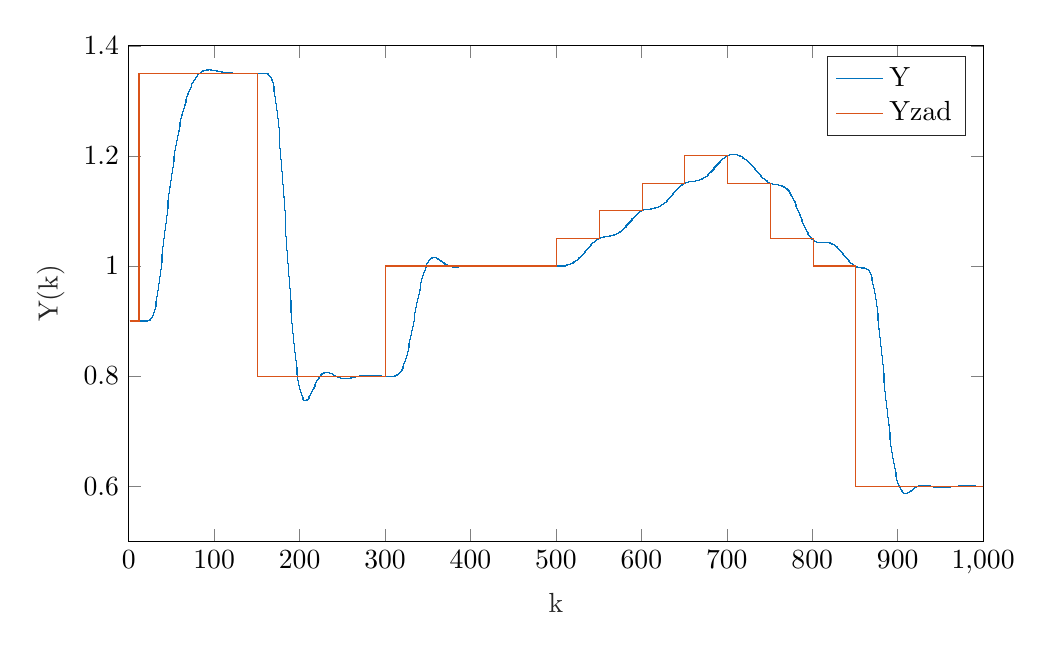
\begin{tikzpicture}

\begin{axis}[%
width=4.272in,
height=2.477in,
at={(0.717in,0.437in)},
scale only axis,
xmin=0,
xmax=1000,
xlabel style={font=\color{white!15!black}},
xlabel={k},
ymin=0.5,
ymax=1.4,
ylabel style={font=\color{white!15!black}},
ylabel={Y(k)},
axis background/.style={fill=white},
legend style={legend cell align=left, align=left, draw=white!15!black}
]
\addplot[const plot, color=mycolor1] table[row sep=crcr] {%
1	0.9\\
2	0.9\\
3	0.9\\
4	0.9\\
5	0.9\\
6	0.9\\
7	0.9\\
8	0.9\\
9	0.9\\
10	0.9\\
11	0.9\\
12	0.9\\
13	0.9\\
14	0.9\\
15	0.9\\
16	0.9\\
17	0.9\\
18	0.9\\
19	0.9\\
20	0.9\\
21	0.9\\
22	0.9003968325\\
23	0.90110505465075\\
24	0.901851548804444\\
25	0.902926732649044\\
26	0.9045740507257\\
27	0.906995673734868\\
28	0.910357581452216\\
29	0.91479409195594\\
30	0.92041189372332\\
31	0.927293631597811\\
32	0.935481917271842\\
33	0.944987479442384\\
34	0.955752143856375\\
35	0.967585143897724\\
36	0.980245690511738\\
37	0.993524900254613\\
38	1.00724220273058\\
39	1.02124212187654\\
40	1.03539139393444\\
41	1.04957638853821\\
42	1.06370080258905\\
43	1.07768359953247\\
44	1.09145716931113\\
45	1.10496568667539\\
46	1.11816364771215\\
47	1.13101456642337\\
48	1.1434898149686\\
49	1.15556759279779\\
50	1.16723201135847\\
51	1.17847228237882\\
52	1.18928199891931\\
53	1.19965849946121\\
54	1.20960230627283\\
55	1.21911663017192\\
56	1.22820693459549\\
57	1.23688055260421\\
58	1.24514635109392\\
59	1.25301443706996\\
60	1.26049590136546\\
61	1.26760259565856\\
62	1.27434693907117\\
63	1.28074174608457\\
64	1.28679954411603\\
65	1.29253204733993\\
66	1.29795023797434\\
67	1.3030644413896\\
68	1.3078843950437\\
69	1.31241931135295\\
70	1.31667793468543\\
71	1.32066859272397\\
72	1.32439924248811\\
73	1.32787751157148\\
74	1.33111076093811\\
75	1.33410618724198\\
76	1.33687093004876\\
77	1.33941215850932\\
78	1.34173714007823\\
79	1.34385329361559\\
80	1.34576822897515\\
81	1.34748977496456\\
82	1.34902599736423\\
83	1.3503852084965\\
84	1.35157596840274\\
85	1.35260707550363\\
86	1.35348754538761\\
87	1.35422657910142\\
88	1.3548335232566\\
89	1.35531782394082\\
90	1.35568897613632\\
91	1.35595647009444\\
92	1.35612973589315\\
93	1.35621808720922\\
94	1.35623066522872\\
95	1.35617638368734\\
96	1.35606387616748\\
97	1.35590144675004\\
98	1.35569702492415\\
99	1.35545812544111\\
100	1.35519181361515\\
101	1.35490467641866\\
102	1.35460279958943\\
103	1.35429175085935\\
104	1.35397656932081\\
105	1.35366176085724\\
106	1.35335129946519\\
107	1.35304863419235\\
108	1.35275670132403\\
109	1.35247794137879\\
110	1.35221432042028\\
111	1.35196735515504\\
112	1.35173814126113\\
113	1.35152738437876\\
114	1.35133543318901\\
115	1.35116231400986\\
116	1.35100776635043\\
117	1.35087127888471\\
118	1.35075212533525\\
119	1.35064939979385\\
120	1.35056205104808\\
121	1.35048891552808\\
122	1.35042874853686\\
123	1.35038025347687\\
124	1.35034210883664\\
125	1.35031299275196\\
126	1.35029160500585\\
127	1.3502766863805\\
128	1.35026703532044\\
129	1.35026152190965\\
130	1.35025909920554\\
131	1.35025881200833\\
132	1.35025980317699\\
133	1.35026131763001\\
134	1.3502627041929\\
135	1.35026341547329\\
136	1.35026300595865\\
137	1.35026112854246\\
138	1.35025752969034\\
139	1.35025204346031\\
140	1.35024458458987\\
141	1.35023514085807\\
142	1.35022376492329\\
143	1.35021056582744\\
144	1.35019570034494\\
145	1.35017936434093\\
146	1.35016178428769\\
147	1.35014320907172\\
148	1.35012390220676\\
149	1.35010413455032\\
150	1.35008417760403\\
151	1.35006429746031\\
152	1.35004474944139\\
153	1.35002577346057\\
154	1.35000759012025\\
155	1.34999039754741\\
156	1.34997436895457\\
157	1.34995965090253\\
158	1.34994636223132\\
159	1.34993459361745\\
160	1.34992440770813\\
161	1.34951889923522\\
162	1.34880333328902\\
163	1.34801637133565\\
164	1.34680623564434\\
165	1.34487818982496\\
166	1.34198761101855\\
167	1.33793381210464\\
168	1.33255453756716\\
169	1.32572106414159\\
170	1.31733384413307\\
171	1.30733781596696\\
172	1.29571365605078\\
173	1.2824452175893\\
174	1.26753853904809\\
175	1.25104365760431\\
176	1.23304727100621\\
177	1.21366635998876\\
178	1.19304265516873\\
179	1.1713378458413\\
180	1.14872944006864\\
181	1.12540626923593\\
182	1.10156388099674\\
183	1.07740205013679\\
184	1.05312296740804\\
185	1.02892759572966\\
186	1.00501147782133\\
187	0.98156127181985\\
188	0.958751911430767\\
189	0.936744301032577\\
190	0.915683468219405\\
191	0.895697151551403\\
192	0.87689483720541\\
193	0.859367140555324\\
194	0.843185398442461\\
195	0.828401526929037\\
196	0.815048252072926\\
197	0.803139700616667\\
198	0.792672284955702\\
199	0.783625826910249\\
200	0.775964873487657\\
201	0.769640163035288\\
202	0.764590200971363\\
203	0.760742909007944\\
204	0.758017323223758\\
205	0.75632531988144\\
206	0.755573340172202\\
207	0.755664080816826\\
208	0.75649812124768\\
209	0.757975463734339\\
210	0.759996967501476\\
211	0.762465661879657\\
212	0.765287927215516\\
213	0.768374535670495\\
214	0.771641546661306\\
215	0.775011053627311\\
216	0.778411780963361\\
217	0.781779532677985\\
218	0.785057497075944\\
219	0.78819641406661\\
220	0.791154613532383\\
221	0.793897934635967\\
222	0.79639953705089\\
223	0.798639615895301\\
224	0.800605032685999\\
225	0.802288874976543\\
226	0.803689957519954\\
227	0.804812277764049\\
228	0.805664438217677\\
229	0.80625904773855\\
230	0.806612113128949\\
231	0.80674243162307\\
232	0.806670993941009\\
233	0.806420406597751\\
234	0.806014341115425\\
235	0.805477016712229\\
236	0.804832721946634\\
237	0.80410537969662\\
238	0.803318158769883\\
239	0.802493134391884\\
240	0.801650998821049\\
241	0.800810822407754\\
242	0.799989864555977\\
243	0.799203433271251\\
244	0.798464791291063\\
245	0.79778510619742\\
246	0.797173441408183\\
247	0.796636784534522\\
248	0.796180109276034\\
249	0.795806466800069\\
250	0.795517102413963\\
251	0.795311593282831\\
252	0.795188002965221\\
253	0.795143048627405\\
254	0.795172276946966\\
255	0.795270244919908\\
256	0.795430702034841\\
257	0.795646770564863\\
258	0.795911121044516\\
259	0.796216140337837\\
260	0.796554090056421\\
261	0.796917253446428\\
262	0.797298069223946\\
263	0.797689251192951\\
264	0.798083892823816\\
265	0.79847555629814\\
266	0.798858345833424\\
267	0.799226965385318\\
268	0.799576761083186\\
269	0.799903748984284\\
270	0.800204628931693\\
271	0.800476785470349\\
272	0.800718276913917\\
273	0.800927813763172\\
274	0.801104727754768\\
275	0.801248932869047\\
276	0.801360879648473\\
277	0.801441504176269\\
278	0.801492173040124\\
279	0.801514625560706\\
280	0.801510914501775\\
281	0.801483346400498\\
282	0.801434422565709\\
283	0.801366781691079\\
284	0.801283144921891\\
285	0.80118626410091\\
286	0.80107887380304\\
287	0.80096364765217\\
288	0.800843159298981\\
289	0.800719848327149\\
290	0.800595991249099\\
291	0.800473677652468\\
292	0.800354791466003\\
293	0.800240997229543\\
294	0.800133731177851\\
295	0.800034196882735\\
296	0.799943365142501\\
297	0.799861977762359\\
298	0.799790554833885\\
299	0.799729405095798\\
300	0.799678638941685\\
301	0.799638183632529\\
302	0.799607800272158\\
303	0.799587102111522\\
304	0.799575573762118\\
305	0.79957259091919\\
306	0.799577440220629\\
307	0.799589338896979\\
308	0.799607453900748\\
309	0.799630920238458\\
310	0.799658858265823\\
311	0.800087252030063\\
312	0.800829896899739\\
313	0.801526913554124\\
314	0.802314448958003\\
315	0.803306971242467\\
316	0.804599897685075\\
317	0.80627193853803\\
318	0.808387185421943\\
319	0.810996970220403\\
320	0.814141517893137\\
321	0.817832237576928\\
322	0.822058342893119\\
323	0.82682333598127\\
324	0.832134339197458\\
325	0.837981296502411\\
326	0.844339788339714\\
327	0.851173479010461\\
328	0.858436240883071\\
329	0.866073994644319\\
330	0.874026300243561\\
331	0.882228655782662\\
332	0.890615216678407\\
333	0.899119386465001\\
334	0.907673219149908\\
335	0.916208290634322\\
336	0.924657350987353\\
337	0.932955694514448\\
338	0.941042287608186\\
339	0.948860689023248\\
340	0.956359792560657\\
341	0.963494373316752\\
342	0.970225388345921\\
343	0.976520118682778\\
344	0.982352309401972\\
345	0.98770229142151\\
346	0.992556980678792\\
347	0.996909733881368\\
348	1.00076008658177\\
349	1.00411339535527\\
350	1.00698040247153\\
351	1.00937674072753\\
352	1.01132239913817\\
353	1.01284116803809\\
354	1.0139600704795\\
355	1.01470878044002\\
356	1.01511903420175\\
357	1.01522404704477\\
358	1.01505794707236\\
359	1.0146552357442\\
360	1.01405028282807\\
361	1.01327686182708\\
362	1.01236773018765\\
363	1.01135425681932\\
364	1.01026609835369\\
365	1.00913092530819\\
366	1.0079741990589\\
367	1.00681899971261\\
368	1.0056859039023\\
369	1.00459291058741\\
370	1.00355541218626\\
371	1.00258620777425\\
372	1.00169555464129\\
373	1.00089125422008\\
374	1.00017876824074\\
375	0.999561360866317\\
376	0.99904026247886\\
377	0.99861485074555\\
378	0.998282844636035\\
379	0.998040507192143\\
380	0.997882853054599\\
381	0.997803857012575\\
382	0.99779666014669\\
383	0.997853770470491\\
384	0.997967255326939\\
385	0.998128923157442\\
386	0.998330492628963\\
387	0.99856374747751\\
388	0.998820675798544\\
389	0.99909359287906\\
390	0.99937524701533\\
391	0.999658908088884\\
392	0.999938438976968\\
393	1.00020835014948\\
394	1.00046383805041\\
395	1.00070080807695\\
396	1.0009158831536\\
397	1.00110639905052\\
398	1.00127038771589\\
399	1.00140654998108\\
400	1.00151421905542\\
401	1.00159331625788\\
402	1.00164430043515\\
403	1.00166811249474\\
404	1.00166611643787\\
405	1.00164003821447\\
406	1.00159190364311\\
407	1.00152397654534\\
408	1.00143869813951\\
409	1.00133862862597\\
410	1.00122639177664\\
411	1.00110462321982\\
412	1.00097592298746\\
413	1.00084281277039\\
414	1.00070769820757\\
415	1.00057283642144\\
416	1.00044030890337\\
417	1.00031199975319\\
418	1.00018957918462\\
419	1.00007449212675\\
420	0.999967951678888\\
421	0.999870937114806\\
422	0.999784196080508\\
423	0.999708250589163\\
424	0.99964340638599\\
425	0.999589765235247\\
426	0.999547239670111\\
427	0.99951556974366\\
428	0.999494341324697\\
429	0.99948300549489\\
430	0.999480898622941\\
431	0.999487262716258\\
432	0.999501265680006\\
433	0.99952202114661\\
434	0.999548607574855\\
435	0.999580086355753\\
436	0.999615518701678\\
437	0.999653981134935\\
438	0.999694579431357\\
439	0.999736460913058\\
440	0.999778825021436\\
441	0.999820932136559\\
442	0.999862110641679\\
443	0.999901762261401\\
444	0.999939365728923\\
445	0.999974478861247\\
446	1.0000067391416\\
447	1.00003586292502\\
448	1.00006164339664\\
449	1.00008394742205\\
450	1.0001027114364\\
451	1.0001179365222\\
452	1.0001296828272\\
453	1.00013806347171\\
454	1.00014323809091\\
455	1.00014540615114\\
456	1.00014480017174\\
457	1.0001416789738\\
458	1.00013632106689\\
459	1.0001290182729\\
460	1.00012006967369\\
461	1.00010977595652\\
462	1.00009843421817\\
463	1.00008633327581\\
464	1.00007374952002\\
465	1.00006094333331\\
466	1.0000481560859\\
467	1.00003560770982\\
468	1.00002349484263\\
469	1.00001198952323\\
470	1.00000123841427\\
471	0.999991362519225\\
472	0.999982457356436\\
473	0.999974593547984\\
474	0.999967817777953\\
475	0.999962154072194\\
476	0.999957605350476\\
477	0.999954155201463\\
478	0.999951769831483\\
479	0.999950400139309\\
480	0.999949983871121\\
481	0.99995044781243\\
482	0.999951709976786\\
483	0.999953681754603\\
484	0.999956269989249\\
485	0.999959378951586\\
486	0.999962912188326\\
487	0.999966774223801\\
488	0.999970872098985\\
489	0.999975116735722\\
490	0.999979424118093\\
491	0.99998371628665\\
492	0.999987922144747\\
493	0.999991978079466\\
494	0.99999582840252\\
495	0.99999942561911\\
496	1.00000273053496\\
497	1.00000571221353\\
498	1.00000834779705\\
499	1.00001062220599\\
500	1.00001252773249\\
501	1.00001406354371\\
502	1.00001523511121\\
503	1.00001605358234\\
504	1.00001653510923\\
505	1.00001670015035\\
506	1.0000165727588\\
507	1.00001617987058\\
508	1.00001555060467\\
509	1.00001471558604\\
510	1.00001370630078\\
511	1.00040938687002\\
512	1.00111634385559\\
513	1.00172392016373\\
514	1.00227704645393\\
515	1.00281406265013\\
516	1.00336749042988\\
517	1.00396472359866\\
518	1.00462864462469\\
519	1.005378174803\\
520	1.00622876478752\\
521	1.0071736562442\\
522	1.00818959391501\\
523	1.00927499574596\\
524	1.01044285867689\\
525	1.01170039690845\\
526	1.01304992484452\\
527	1.01448962762909\\
528	1.01601423267138\\
529	1.01761559400932\\
530	1.01928319999231\\
531	1.0210055401198\\
532	1.02277202429034\\
533	1.0245727687922\\
534	1.02639697486112\\
535	1.02823262041945\\
536	1.0300670318369\\
537	1.03188736390347\\
538	1.03368100073895\\
539	1.03543588868484\\
540	1.03714081076041\\
541	1.03878556621624\\
542	1.04036099084052\\
543	1.04185889769697\\
544	1.0432721046191\\
545	1.0445945486784\\
546	1.04582138463271\\
547	1.04694903207134\\
548	1.04797517997097\\
549	1.04889875606294\\
550	1.04971986728836\\
551	1.05043971882005\\
552	1.05106052379489\\
553	1.05158541486351\\
554	1.05201835689525\\
555	1.05236405258994\\
556	1.05262783779425\\
557	1.05281556975452\\
558	1.05293351269471\\
559	1.05298822431716\\
560	1.05298644616155\\
561	1.05333263244468\\
562	1.05394921456856\\
563	1.05443231932367\\
564	1.05483302951003\\
565	1.05519562267473\\
566	1.05555827515993\\
567	1.05595369385869\\
568	1.05640968435715\\
569	1.05694966297499\\
570	1.05759311919599\\
571	1.05833682011125\\
572	1.05916046354588\\
573	1.06006488133588\\
574	1.06106501687024\\
575	1.06216959444918\\
576	1.06338201723138\\
577	1.06470115866325\\
578	1.06612205987656\\
579	1.06763654398343\\
580	1.06923375684288\\
581	1.07090157113358\\
582	1.07262854843728\\
583	1.07440376931444\\
584	1.07621525118013\\
585	1.07804967488953\\
586	1.07989298958076\\
587	1.08173092445078\\
588	1.08354941970057\\
589	1.08533498728995\\
590	1.0870750107602\\
591	1.0887579473229\\
592	1.09037336741601\\
593	1.09191191109257\\
594	1.09336532773929\\
595	1.09472659976837\\
596	1.09599004756228\\
597	1.09715138050907\\
598	1.09820770296188\\
599	1.09915748268227\\
600	1.1000004882354\\
601	1.10073770303673\\
602	1.10137122845058\\
603	1.10190418733924\\
604	1.10234062769767\\
605	1.10268541839338\\
606	1.10294413404599\\
607	1.10312293249677\\
608	1.1032284294665\\
609	1.10326757419677\\
610	1.10324752919333\\
611	1.10357322078997\\
612	1.10416755575576\\
613	1.10462710229684\\
614	1.10500337757068\\
615	1.1053410795647\\
616	1.10567878457563\\
617	1.10604957333897\\
618	1.10648159450064\\
619	1.10699857293944\\
620	1.10762026941351\\
621	1.10834368157685\\
622	1.10914869493528\\
623	1.11003628786775\\
624	1.11102151121821\\
625	1.11211315872286\\
626	1.11331466659475\\
627	1.1146249071052\\
628	1.11603888856487\\
629	1.1175483725503\\
630	1.11914241786794\\
631	1.12080878808583\\
632	1.12253591731215\\
633	1.12431274396181\\
634	1.12612713213262\\
635	1.12796560154174\\
636	1.12981393559359\\
637	1.1316576962092\\
638	1.13348265761338\\
639	1.13527516968724\\
640	1.13702246011925\\
641	1.1387128385308\\
642	1.14033573775641\\
643	1.14188167163494\\
644	1.1433422758195\\
645	1.1447104322657\\
646	1.145980374691\\
647	1.14714773985568\\
648	1.14820957351633\\
649	1.14916429863164\\
650	1.15001165231066\\
651	1.15075259922795\\
652	1.15138923393206\\
653	1.15192468347357\\
654	1.15236301001512\\
655	1.15270910546886\\
656	1.15296857522063\\
657	1.15314761441455\\
658	1.15325288141846\\
659	1.15329137228585\\
660	1.15327029935151\\
661	1.15359464542537\\
662	1.15418737495578\\
663	1.15464510835916\\
664	1.15501941276866\\
665	1.15535503460211\\
666	1.155690596331\\
667	1.15605922200227\\
668	1.15648910020565\\
669	1.1570039919949\\
670	1.1576236902334\\
671	1.15834522017804\\
672	1.1591484900928\\
673	1.16003449649167\\
674	1.16101830408993\\
675	1.16210871639956\\
676	1.16330917547781\\
677	1.16461855572892\\
678	1.1660318641527\\
679	1.16754085787656\\
680	1.16913458845456\\
681	1.17080080976581\\
682	1.17252794419407\\
683	1.17430491679859\\
684	1.17611957706646\\
685	1.17795842920068\\
686	1.17980724052501\\
687	1.18165155663356\\
688	1.183477135477\\
689	1.18527031098941\\
690	1.18701829548606\\
691	1.1887093840055\\
692	1.19033299577327\\
693	1.19187963214186\\
694	1.19334091751603\\
695	1.1947097239258\\
696	1.19598027654118\\
697	1.1971482049811\\
698	1.19821054926872\\
699	1.19916572801499\\
700	1.20001347532299\\
701	1.20075475413974\\
702	1.20139165848492\\
703	1.20192731598551\\
704	1.20236579038155\\
705	1.20271197605165\\
706	1.20297148161954\\
707	1.20315050611813\\
708	1.2032557123336\\
709	1.20329410114738\\
710	1.20327289001505\\
711	1.20280340246781\\
712	1.20197949443207\\
713	1.20121916410976\\
714	1.20048418239853\\
715	1.19974267734762\\
716	1.19896828523762\\
717	1.19813939477381\\
718	1.19723847653431\\
719	1.19625149024025\\
720	1.19516736283582\\
721	1.1939966656711\\
722	1.19276584118506\\
723	1.19147906815355\\
724	1.19012543003654\\
725	1.18869930913946\\
726	1.18719952083662\\
727	1.18562856671054\\
728	1.18399199220324\\
729	1.18229783590438\\
730	1.18055615898757\\
731	1.17877771994491\\
732	1.17697210277387\\
733	1.17514797964956\\
734	1.17331477603314\\
735	1.17148301795\\
736	1.16966379732088\\
737	1.16786832757869\\
738	1.16610757631066\\
739	1.16439196343536\\
740	1.16273111497917\\
741	1.16113370855843\\
742	1.15960747443339\\
743	1.15815927213312\\
744	1.1567950765124\\
745	1.15551987346826\\
746	1.15433756859892\\
747	1.15325094422691\\
748	1.15226165621367\\
749	1.15137026334976\\
750	1.15057628326406\\
751	1.14987826762436\\
752	1.14927388477541\\
753	1.14875999903333\\
754	1.14833274762912\\
755	1.14798762385052\\
756	1.14771956985092\\
757	1.14752307614174\\
758	1.14739228361596\\
759	1.14732108472827\\
760	1.14730322110229\\
761	1.14693478039478\\
762	1.14629387728537\\
763	1.14576769479887\\
764	1.1452749569674\\
765	1.14474622511151\\
766	1.14412257054753\\
767	1.1433543874333\\
768	1.14240033028543\\
769	1.14122636251588\\
770	1.13980490394141\\
771	1.13813327881775\\
772	1.13622775539906\\
773	1.13408590561064\\
774	1.13169482228744\\
775	1.12905159646821\\
776	1.12616177549122\\
777	1.12303801303747\\
778	1.11969888827224\\
779	1.1161678739883\\
780	1.1124724360704\\
781	1.10864232036899\\
782	1.10470732601222\\
783	1.10069720924071\\
784	1.09664292622671\\
785	1.0925765150098\\
786	1.08853013218155\\
787	1.08453524608933\\
788	1.08062196520243\\
789	1.07681848310651\\
790	1.07315062404299\\
791	1.06964151989627\\
792	1.06631147833079\\
793	1.0631779602663\\
794	1.06025550341444\\
795	1.05755559675842\\
796	1.05508660916733\\
797	1.05285380248214\\
798	1.05085941456476\\
799	1.04910279996318\\
800	1.04758061769505\\
801	1.04628705506404\\
802	1.0452140722705\\
803	1.044351653951\\
804	1.04368806551219\\
805	1.0432101193333\\
806	1.04290345062832\\
807	1.04275279655942\\
808	1.04274227153947\\
809	1.04285563294737\\
810	1.04307653255715\\
811	1.04299140055327\\
812	1.04266965616485\\
813	1.04250699534601\\
814	1.04244392825164\\
815	1.04242839530598\\
816	1.04241511838254\\
817	1.04236500994948\\
818	1.04224463192628\\
819	1.0420256973767\\
820	1.04168460935379\\
821	1.04122123254866\\
822	1.04065317567022\\
823	1.03997755132816\\
824	1.0391780176565\\
825	1.03824509623151\\
826	1.03717522005222\\
827	1.03596988412573\\
828	1.03463488734745\\
829	1.03317965587997\\
830	1.03161663952905\\
831	1.02995984594171\\
832	1.02822282091232\\
833	1.02641876520716\\
834	1.02456206402348\\
835	1.02266850710263\\
836	1.02075463337065\\
837	1.01883717345544\\
838	1.01693257809918\\
839	1.01505662198516\\
840	1.01322407378949\\
841	1.01144846921064\\
842	1.00974205151795\\
843	1.00811579985152\\
844	1.00657937856382\\
845	1.00514100699203\\
846	1.00380735230144\\
847	1.00258348023216\\
848	1.00147285448576\\
849	1.00047737674732\\
850	0.999597460423544\\
851	0.998832129947184\\
852	0.998179132813485\\
853	0.997635052547799\\
854	0.99719542259527\\
855	0.996854848745601\\
856	0.996607142692001\\
857	0.996445462924645\\
858	0.996362458044904\\
859	0.996350408427594\\
860	0.996401362874079\\
861	0.996109629816194\\
862	0.995551614064934\\
863	0.995009666148765\\
864	0.994216691386937\\
865	0.992947798135629\\
866	0.991015297256109\\
867	0.988264238824071\\
868	0.984568429788473\\
869	0.979826882167447\\
870	0.973960646650634\\
871	0.966929205462071\\
872	0.958722682741073\\
873	0.949327563251365\\
874	0.938742061889922\\
875	0.926997470478845\\
876	0.914152732667802\\
877	0.900289718232804\\
878	0.885526609339621\\
879	0.870048740470661\\
880	0.854065600402944\\
881	0.837757545633109\\
882	0.821279147033163\\
883	0.804762184475895\\
884	0.788321943064686\\
885	0.772069348052869\\
886	0.756116297553503\\
887	0.740572555930676\\
888	0.725542316593946\\
889	0.711118753508792\\
890	0.697379335889381\\
891	0.684385756488678\\
892	0.672186159185987\\
893	0.660817075710471\\
894	0.650304933391636\\
895	0.640666706305716\\
896	0.631909779237839\\
897	0.62403174813625\\
898	0.617020556497771\\
899	0.610855074757561\\
900	0.605506172482791\\
901	0.600938020907226\\
902	0.597109302249915\\
903	0.593974236039276\\
904	0.591483458059632\\
905	0.589584813766831\\
906	0.588224143381368\\
907	0.587346096947157\\
908	0.586894964978029\\
909	0.586815487083717\\
910	0.587053594013179\\
911	0.587557049286112\\
912	0.588275984373666\\
913	0.5891633404078\\
914	0.590175231538074\\
915	0.591271240227415\\
916	0.592414648094076\\
917	0.593572600485164\\
918	0.594716201925493\\
919	0.595820542082976\\
920	0.596864655766684\\
921	0.597831424121497\\
922	0.598707425980132\\
923	0.599482747943879\\
924	0.600150760422345\\
925	0.600707865682163\\
926	0.60115322333697\\
927	0.601488458671674\\
928	0.60171735945684\\
929	0.601845567099499\\
930	0.601880267866927\\
931	0.601829889460008\\
932	0.601703807504322\\
933	0.601512065760973\\
934	0.601265113179839\\
935	0.60097356035893\\
936	0.600647957498086\\
937	0.600298595488258\\
938	0.599935331317265\\
939	0.599567438488636\\
940	0.599203482659606\\
941	0.598851222237878\\
942	0.598517533261986\\
943	0.598208357540609\\
944	0.597928672739817\\
945	0.597682482873989\\
946	0.597472827466267\\
947	0.597301807492771\\
948	0.597170626110886\\
949	0.597079642097725\\
950	0.597028433891878\\
951	0.597015872139279\\
952	0.597040198688923\\
953	0.597099110061235\\
954	0.597189843515262\\
955	0.597309263965637\\
956	0.597453950142212\\
957	0.597620278541056\\
958	0.597804503881963\\
959	0.598002834961496\\
960	0.598211504968482\\
961	0.598426835507268\\
962	0.598645293749683\\
963	0.598863542306555\\
964	0.599078481571407\\
965	0.599287284440605\\
966	0.599487423454155\\
967	0.599676690528423\\
968	0.599853209565049\\
969	0.600015442318847\\
970	0.60016218799078\\
971	0.600292577080268\\
972	0.600406060084125\\
973	0.600502391667822\\
974	0.600581610959129\\
975	0.600644018625313\\
976	0.600690151394004\\
977	0.600720754665501\\
978	0.600736753842057\\
979	0.600739224968596\\
980	0.60072936524077\\
981	0.600708463891536\\
982	0.600677873917782\\
983	0.60063898505529\\
984	0.600593198354631\\
985	0.600541902653678\\
986	0.600486453185301\\
987	0.600428152502531\\
988	0.600368233848821\\
989	0.600307847048944\\
990	0.600248046947038\\
991	0.600189784373033\\
992	0.600133899577584\\
993	0.600081118039004\\
994	0.600032048513815\\
995	0.599987183175549\\
996	0.599946899664326\\
997	0.599911464852545\\
998	0.599881040119561\\
999	0.599855687920309\\
1000	0.599835379429238\\
};
\addlegendentry{Y}

\addplot[const plot, color=mycolor2] table[row sep=crcr] {%
1	0.9\\
2	0.9\\
3	0.9\\
4	0.9\\
5	0.9\\
6	0.9\\
7	0.9\\
8	0.9\\
9	0.9\\
10	0.9\\
11	0.9\\
12	1.35\\
13	1.35\\
14	1.35\\
15	1.35\\
16	1.35\\
17	1.35\\
18	1.35\\
19	1.35\\
20	1.35\\
21	1.35\\
22	1.35\\
23	1.35\\
24	1.35\\
25	1.35\\
26	1.35\\
27	1.35\\
28	1.35\\
29	1.35\\
30	1.35\\
31	1.35\\
32	1.35\\
33	1.35\\
34	1.35\\
35	1.35\\
36	1.35\\
37	1.35\\
38	1.35\\
39	1.35\\
40	1.35\\
41	1.35\\
42	1.35\\
43	1.35\\
44	1.35\\
45	1.35\\
46	1.35\\
47	1.35\\
48	1.35\\
49	1.35\\
50	1.35\\
51	1.35\\
52	1.35\\
53	1.35\\
54	1.35\\
55	1.35\\
56	1.35\\
57	1.35\\
58	1.35\\
59	1.35\\
60	1.35\\
61	1.35\\
62	1.35\\
63	1.35\\
64	1.35\\
65	1.35\\
66	1.35\\
67	1.35\\
68	1.35\\
69	1.35\\
70	1.35\\
71	1.35\\
72	1.35\\
73	1.35\\
74	1.35\\
75	1.35\\
76	1.35\\
77	1.35\\
78	1.35\\
79	1.35\\
80	1.35\\
81	1.35\\
82	1.35\\
83	1.35\\
84	1.35\\
85	1.35\\
86	1.35\\
87	1.35\\
88	1.35\\
89	1.35\\
90	1.35\\
91	1.35\\
92	1.35\\
93	1.35\\
94	1.35\\
95	1.35\\
96	1.35\\
97	1.35\\
98	1.35\\
99	1.35\\
100	1.35\\
101	1.35\\
102	1.35\\
103	1.35\\
104	1.35\\
105	1.35\\
106	1.35\\
107	1.35\\
108	1.35\\
109	1.35\\
110	1.35\\
111	1.35\\
112	1.35\\
113	1.35\\
114	1.35\\
115	1.35\\
116	1.35\\
117	1.35\\
118	1.35\\
119	1.35\\
120	1.35\\
121	1.35\\
122	1.35\\
123	1.35\\
124	1.35\\
125	1.35\\
126	1.35\\
127	1.35\\
128	1.35\\
129	1.35\\
130	1.35\\
131	1.35\\
132	1.35\\
133	1.35\\
134	1.35\\
135	1.35\\
136	1.35\\
137	1.35\\
138	1.35\\
139	1.35\\
140	1.35\\
141	1.35\\
142	1.35\\
143	1.35\\
144	1.35\\
145	1.35\\
146	1.35\\
147	1.35\\
148	1.35\\
149	1.35\\
150	1.35\\
151	0.8\\
152	0.8\\
153	0.8\\
154	0.8\\
155	0.8\\
156	0.8\\
157	0.8\\
158	0.8\\
159	0.8\\
160	0.8\\
161	0.8\\
162	0.8\\
163	0.8\\
164	0.8\\
165	0.8\\
166	0.8\\
167	0.8\\
168	0.8\\
169	0.8\\
170	0.8\\
171	0.8\\
172	0.8\\
173	0.8\\
174	0.8\\
175	0.8\\
176	0.8\\
177	0.8\\
178	0.8\\
179	0.8\\
180	0.8\\
181	0.8\\
182	0.8\\
183	0.8\\
184	0.8\\
185	0.8\\
186	0.8\\
187	0.8\\
188	0.8\\
189	0.8\\
190	0.8\\
191	0.8\\
192	0.8\\
193	0.8\\
194	0.8\\
195	0.8\\
196	0.8\\
197	0.8\\
198	0.8\\
199	0.8\\
200	0.8\\
201	0.8\\
202	0.8\\
203	0.8\\
204	0.8\\
205	0.8\\
206	0.8\\
207	0.8\\
208	0.8\\
209	0.8\\
210	0.8\\
211	0.8\\
212	0.8\\
213	0.8\\
214	0.8\\
215	0.8\\
216	0.8\\
217	0.8\\
218	0.8\\
219	0.8\\
220	0.8\\
221	0.8\\
222	0.8\\
223	0.8\\
224	0.8\\
225	0.8\\
226	0.8\\
227	0.8\\
228	0.8\\
229	0.8\\
230	0.8\\
231	0.8\\
232	0.8\\
233	0.8\\
234	0.8\\
235	0.8\\
236	0.8\\
237	0.8\\
238	0.8\\
239	0.8\\
240	0.8\\
241	0.8\\
242	0.8\\
243	0.8\\
244	0.8\\
245	0.8\\
246	0.8\\
247	0.8\\
248	0.8\\
249	0.8\\
250	0.8\\
251	0.8\\
252	0.8\\
253	0.8\\
254	0.8\\
255	0.8\\
256	0.8\\
257	0.8\\
258	0.8\\
259	0.8\\
260	0.8\\
261	0.8\\
262	0.8\\
263	0.8\\
264	0.8\\
265	0.8\\
266	0.8\\
267	0.8\\
268	0.8\\
269	0.8\\
270	0.8\\
271	0.8\\
272	0.8\\
273	0.8\\
274	0.8\\
275	0.8\\
276	0.8\\
277	0.8\\
278	0.8\\
279	0.8\\
280	0.8\\
281	0.8\\
282	0.8\\
283	0.8\\
284	0.8\\
285	0.8\\
286	0.8\\
287	0.8\\
288	0.8\\
289	0.8\\
290	0.8\\
291	0.8\\
292	0.8\\
293	0.8\\
294	0.8\\
295	0.8\\
296	0.8\\
297	0.8\\
298	0.8\\
299	0.8\\
300	0.8\\
301	1\\
302	1\\
303	1\\
304	1\\
305	1\\
306	1\\
307	1\\
308	1\\
309	1\\
310	1\\
311	1\\
312	1\\
313	1\\
314	1\\
315	1\\
316	1\\
317	1\\
318	1\\
319	1\\
320	1\\
321	1\\
322	1\\
323	1\\
324	1\\
325	1\\
326	1\\
327	1\\
328	1\\
329	1\\
330	1\\
331	1\\
332	1\\
333	1\\
334	1\\
335	1\\
336	1\\
337	1\\
338	1\\
339	1\\
340	1\\
341	1\\
342	1\\
343	1\\
344	1\\
345	1\\
346	1\\
347	1\\
348	1\\
349	1\\
350	1\\
351	1\\
352	1\\
353	1\\
354	1\\
355	1\\
356	1\\
357	1\\
358	1\\
359	1\\
360	1\\
361	1\\
362	1\\
363	1\\
364	1\\
365	1\\
366	1\\
367	1\\
368	1\\
369	1\\
370	1\\
371	1\\
372	1\\
373	1\\
374	1\\
375	1\\
376	1\\
377	1\\
378	1\\
379	1\\
380	1\\
381	1\\
382	1\\
383	1\\
384	1\\
385	1\\
386	1\\
387	1\\
388	1\\
389	1\\
390	1\\
391	1\\
392	1\\
393	1\\
394	1\\
395	1\\
396	1\\
397	1\\
398	1\\
399	1\\
400	1\\
401	1\\
402	1\\
403	1\\
404	1\\
405	1\\
406	1\\
407	1\\
408	1\\
409	1\\
410	1\\
411	1\\
412	1\\
413	1\\
414	1\\
415	1\\
416	1\\
417	1\\
418	1\\
419	1\\
420	1\\
421	1\\
422	1\\
423	1\\
424	1\\
425	1\\
426	1\\
427	1\\
428	1\\
429	1\\
430	1\\
431	1\\
432	1\\
433	1\\
434	1\\
435	1\\
436	1\\
437	1\\
438	1\\
439	1\\
440	1\\
441	1\\
442	1\\
443	1\\
444	1\\
445	1\\
446	1\\
447	1\\
448	1\\
449	1\\
450	1\\
451	1\\
452	1\\
453	1\\
454	1\\
455	1\\
456	1\\
457	1\\
458	1\\
459	1\\
460	1\\
461	1\\
462	1\\
463	1\\
464	1\\
465	1\\
466	1\\
467	1\\
468	1\\
469	1\\
470	1\\
471	1\\
472	1\\
473	1\\
474	1\\
475	1\\
476	1\\
477	1\\
478	1\\
479	1\\
480	1\\
481	1\\
482	1\\
483	1\\
484	1\\
485	1\\
486	1\\
487	1\\
488	1\\
489	1\\
490	1\\
491	1\\
492	1\\
493	1\\
494	1\\
495	1\\
496	1\\
497	1\\
498	1\\
499	1\\
500	1\\
501	1.05\\
502	1.05\\
503	1.05\\
504	1.05\\
505	1.05\\
506	1.05\\
507	1.05\\
508	1.05\\
509	1.05\\
510	1.05\\
511	1.05\\
512	1.05\\
513	1.05\\
514	1.05\\
515	1.05\\
516	1.05\\
517	1.05\\
518	1.05\\
519	1.05\\
520	1.05\\
521	1.05\\
522	1.05\\
523	1.05\\
524	1.05\\
525	1.05\\
526	1.05\\
527	1.05\\
528	1.05\\
529	1.05\\
530	1.05\\
531	1.05\\
532	1.05\\
533	1.05\\
534	1.05\\
535	1.05\\
536	1.05\\
537	1.05\\
538	1.05\\
539	1.05\\
540	1.05\\
541	1.05\\
542	1.05\\
543	1.05\\
544	1.05\\
545	1.05\\
546	1.05\\
547	1.05\\
548	1.05\\
549	1.05\\
550	1.05\\
551	1.1\\
552	1.1\\
553	1.1\\
554	1.1\\
555	1.1\\
556	1.1\\
557	1.1\\
558	1.1\\
559	1.1\\
560	1.1\\
561	1.1\\
562	1.1\\
563	1.1\\
564	1.1\\
565	1.1\\
566	1.1\\
567	1.1\\
568	1.1\\
569	1.1\\
570	1.1\\
571	1.1\\
572	1.1\\
573	1.1\\
574	1.1\\
575	1.1\\
576	1.1\\
577	1.1\\
578	1.1\\
579	1.1\\
580	1.1\\
581	1.1\\
582	1.1\\
583	1.1\\
584	1.1\\
585	1.1\\
586	1.1\\
587	1.1\\
588	1.1\\
589	1.1\\
590	1.1\\
591	1.1\\
592	1.1\\
593	1.1\\
594	1.1\\
595	1.1\\
596	1.1\\
597	1.1\\
598	1.1\\
599	1.1\\
600	1.1\\
601	1.15\\
602	1.15\\
603	1.15\\
604	1.15\\
605	1.15\\
606	1.15\\
607	1.15\\
608	1.15\\
609	1.15\\
610	1.15\\
611	1.15\\
612	1.15\\
613	1.15\\
614	1.15\\
615	1.15\\
616	1.15\\
617	1.15\\
618	1.15\\
619	1.15\\
620	1.15\\
621	1.15\\
622	1.15\\
623	1.15\\
624	1.15\\
625	1.15\\
626	1.15\\
627	1.15\\
628	1.15\\
629	1.15\\
630	1.15\\
631	1.15\\
632	1.15\\
633	1.15\\
634	1.15\\
635	1.15\\
636	1.15\\
637	1.15\\
638	1.15\\
639	1.15\\
640	1.15\\
641	1.15\\
642	1.15\\
643	1.15\\
644	1.15\\
645	1.15\\
646	1.15\\
647	1.15\\
648	1.15\\
649	1.15\\
650	1.15\\
651	1.2\\
652	1.2\\
653	1.2\\
654	1.2\\
655	1.2\\
656	1.2\\
657	1.2\\
658	1.2\\
659	1.2\\
660	1.2\\
661	1.2\\
662	1.2\\
663	1.2\\
664	1.2\\
665	1.2\\
666	1.2\\
667	1.2\\
668	1.2\\
669	1.2\\
670	1.2\\
671	1.2\\
672	1.2\\
673	1.2\\
674	1.2\\
675	1.2\\
676	1.2\\
677	1.2\\
678	1.2\\
679	1.2\\
680	1.2\\
681	1.2\\
682	1.2\\
683	1.2\\
684	1.2\\
685	1.2\\
686	1.2\\
687	1.2\\
688	1.2\\
689	1.2\\
690	1.2\\
691	1.2\\
692	1.2\\
693	1.2\\
694	1.2\\
695	1.2\\
696	1.2\\
697	1.2\\
698	1.2\\
699	1.2\\
700	1.2\\
701	1.15\\
702	1.15\\
703	1.15\\
704	1.15\\
705	1.15\\
706	1.15\\
707	1.15\\
708	1.15\\
709	1.15\\
710	1.15\\
711	1.15\\
712	1.15\\
713	1.15\\
714	1.15\\
715	1.15\\
716	1.15\\
717	1.15\\
718	1.15\\
719	1.15\\
720	1.15\\
721	1.15\\
722	1.15\\
723	1.15\\
724	1.15\\
725	1.15\\
726	1.15\\
727	1.15\\
728	1.15\\
729	1.15\\
730	1.15\\
731	1.15\\
732	1.15\\
733	1.15\\
734	1.15\\
735	1.15\\
736	1.15\\
737	1.15\\
738	1.15\\
739	1.15\\
740	1.15\\
741	1.15\\
742	1.15\\
743	1.15\\
744	1.15\\
745	1.15\\
746	1.15\\
747	1.15\\
748	1.15\\
749	1.15\\
750	1.15\\
751	1.05\\
752	1.05\\
753	1.05\\
754	1.05\\
755	1.05\\
756	1.05\\
757	1.05\\
758	1.05\\
759	1.05\\
760	1.05\\
761	1.05\\
762	1.05\\
763	1.05\\
764	1.05\\
765	1.05\\
766	1.05\\
767	1.05\\
768	1.05\\
769	1.05\\
770	1.05\\
771	1.05\\
772	1.05\\
773	1.05\\
774	1.05\\
775	1.05\\
776	1.05\\
777	1.05\\
778	1.05\\
779	1.05\\
780	1.05\\
781	1.05\\
782	1.05\\
783	1.05\\
784	1.05\\
785	1.05\\
786	1.05\\
787	1.05\\
788	1.05\\
789	1.05\\
790	1.05\\
791	1.05\\
792	1.05\\
793	1.05\\
794	1.05\\
795	1.05\\
796	1.05\\
797	1.05\\
798	1.05\\
799	1.05\\
800	1.05\\
801	1\\
802	1\\
803	1\\
804	1\\
805	1\\
806	1\\
807	1\\
808	1\\
809	1\\
810	1\\
811	1\\
812	1\\
813	1\\
814	1\\
815	1\\
816	1\\
817	1\\
818	1\\
819	1\\
820	1\\
821	1\\
822	1\\
823	1\\
824	1\\
825	1\\
826	1\\
827	1\\
828	1\\
829	1\\
830	1\\
831	1\\
832	1\\
833	1\\
834	1\\
835	1\\
836	1\\
837	1\\
838	1\\
839	1\\
840	1\\
841	1\\
842	1\\
843	1\\
844	1\\
845	1\\
846	1\\
847	1\\
848	1\\
849	1\\
850	1\\
851	0.6\\
852	0.6\\
853	0.6\\
854	0.6\\
855	0.6\\
856	0.6\\
857	0.6\\
858	0.6\\
859	0.6\\
860	0.6\\
861	0.6\\
862	0.6\\
863	0.6\\
864	0.6\\
865	0.6\\
866	0.6\\
867	0.6\\
868	0.6\\
869	0.6\\
870	0.6\\
871	0.6\\
872	0.6\\
873	0.6\\
874	0.6\\
875	0.6\\
876	0.6\\
877	0.6\\
878	0.6\\
879	0.6\\
880	0.6\\
881	0.6\\
882	0.6\\
883	0.6\\
884	0.6\\
885	0.6\\
886	0.6\\
887	0.6\\
888	0.6\\
889	0.6\\
890	0.6\\
891	0.6\\
892	0.6\\
893	0.6\\
894	0.6\\
895	0.6\\
896	0.6\\
897	0.6\\
898	0.6\\
899	0.6\\
900	0.6\\
901	0.6\\
902	0.6\\
903	0.6\\
904	0.6\\
905	0.6\\
906	0.6\\
907	0.6\\
908	0.6\\
909	0.6\\
910	0.6\\
911	0.6\\
912	0.6\\
913	0.6\\
914	0.6\\
915	0.6\\
916	0.6\\
917	0.6\\
918	0.6\\
919	0.6\\
920	0.6\\
921	0.6\\
922	0.6\\
923	0.6\\
924	0.6\\
925	0.6\\
926	0.6\\
927	0.6\\
928	0.6\\
929	0.6\\
930	0.6\\
931	0.6\\
932	0.6\\
933	0.6\\
934	0.6\\
935	0.6\\
936	0.6\\
937	0.6\\
938	0.6\\
939	0.6\\
940	0.6\\
941	0.6\\
942	0.6\\
943	0.6\\
944	0.6\\
945	0.6\\
946	0.6\\
947	0.6\\
948	0.6\\
949	0.6\\
950	0.6\\
951	0.6\\
952	0.6\\
953	0.6\\
954	0.6\\
955	0.6\\
956	0.6\\
957	0.6\\
958	0.6\\
959	0.6\\
960	0.6\\
961	0.6\\
962	0.6\\
963	0.6\\
964	0.6\\
965	0.6\\
966	0.6\\
967	0.6\\
968	0.6\\
969	0.6\\
970	0.6\\
971	0.6\\
972	0.6\\
973	0.6\\
974	0.6\\
975	0.6\\
976	0.6\\
977	0.6\\
978	0.6\\
979	0.6\\
980	0.6\\
981	0.6\\
982	0.6\\
983	0.6\\
984	0.6\\
985	0.6\\
986	0.6\\
987	0.6\\
988	0.6\\
989	0.6\\
990	0.6\\
991	0.6\\
992	0.6\\
993	0.6\\
994	0.6\\
995	0.6\\
996	0.6\\
997	0.6\\
998	0.6\\
999	0.6\\
1000	0.6\\
};
\addlegendentry{Yzad}

\end{axis}
\end{tikzpicture}%
\caption{Śledzenie wartości zadanej dla parametrów $K = 1,3$, $T_i = 10$, $T_d = 3$}
\end{figure}

Wskaźnik jakości regulacji:

\begin{equation}
E = 20,5988
\end{equation}

\section{Strojenie regulatora DMC}

Dostrojenie regulatora zaczynamy od losowy wybranych parametrów: $N=100$, $N_u=10$, $\lambda=1$.


\begin{figure}[H]
\centering
% This file was created by matlab2tikz.
%
%The latest updates can be retrieved from
%  http://www.mathworks.com/matlabcentral/fileexchange/22022-matlab2tikz-matlab2tikz
%where you can also make suggestions and rate matlab2tikz.
%
\definecolor{mycolor1}{rgb}{0.00000,0.44700,0.74100}%
%
\begin{tikzpicture}

\begin{axis}[%
width=4.272in,
height=2.477in,
at={(0.717in,0.437in)},
scale only axis,
xmin=0,
xmax=1000,
xlabel style={font=\color{white!15!black}},
xlabel={k},
ymin=2.5,
ymax=3.4,
ylabel style={font=\color{white!15!black}},
ylabel={U(k)},
axis background/.style={fill=white}
]
\addplot[const plot, color=mycolor1, forget plot] table[row sep=crcr] {%
1	3\\
2	3\\
3	3\\
4	3\\
5	3\\
6	3\\
7	3\\
8	3\\
9	3\\
10	3\\
11	3\\
12	3.075\\
13	3.15\\
14	3.225\\
15	3.3\\
16	3.3\\
17	3.3\\
18	3.3\\
19	3.3\\
20	3.3\\
21	3.3\\
22	3.3\\
23	3.28931458648346\\
24	3.25133064557951\\
25	3.19524149478313\\
26	3.12904388925288\\
27	3.05978113731898\\
28	2.99338025101242\\
29	2.93458414908846\\
30	2.88695908485366\\
31	2.85295899426662\\
32	2.83381151785739\\
33	2.8294173467011\\
34	2.83860529874281\\
35	2.85950453893816\\
36	2.88984822078149\\
37	2.92721420491786\\
38	2.96920913264412\\
39	3.01360253839825\\
40	3.05841786546152\\
41	3.10198721258691\\
42	3.14297640926035\\
43	3.18038662537081\\
44	3.21353820303552\\
45	3.24204179101837\\
46	3.26576120096762\\
47	3.28477172178124\\
48	3.29931695169033\\
49	3.3\\
50	3.3\\
51	3.3\\
52	3.3\\
53	3.29899230796395\\
54	3.29640050513599\\
55	3.29268175104917\\
56	3.28824251678825\\
57	3.28343241937815\\
58	3.27854167111154\\
59	3.27384639968098\\
60	3.26961954951152\\
61	3.26607940109581\\
62	3.26336138680369\\
63	3.26151505476011\\
64	3.26052000102801\\
65	3.26030611367496\\
66	3.26077071147583\\
67	3.26179270039286\\
68	3.26324393030565\\
69	3.26499798234498\\
70	3.2669366521275\\
71	3.2689544159607\\
72	3.27096117637163\\
73	3.27288358142712\\
74	3.2746652009646\\
75	3.27626582394749\\
76	3.27766011664315\\
77	3.27883585306794\\
78	3.27979189886379\\
79	3.28053609896377\\
80	3.2810831893203\\
81	3.28145282460535\\
82	3.28166778788677\\
83	3.281752425342\\
84	3.28173132937873\\
85	3.28162827719411\\
86	3.28146541877018\\
87	3.2812626984003\\
88	3.28103748743635\\
89	3.28080439932616\\
90	3.28057525812732\\
91	3.28035919025807\\
92	3.28016281018719\\
93	3.2799904727936\\
94	3.27984456791956\\
95	3.27972583591449\\
96	3.2796336864724\\
97	3.27956650660436\\
98	3.27952194659633\\
99	3.27949717699495\\
100	3.27948911180204\\
101	3.27949459548059\\
102	3.2795105534217\\
103	3.27953410715416\\
104	3.27956265680904\\
105	3.27959393421882\\
106	3.27962603057174\\
107	3.27965740280307\\
108	3.27968686293101\\
109	3.27971355438626\\
110	3.27973691908932\\
111	3.27975665863677\\
112	3.27977269250342\\
113	3.27978511568364\\
114	3.27979415770871\\
115	3.27980014451074\\
116	3.27980346417125\\
117	3.27980453720779\\
118	3.27980379171896\\
119	3.27980164343264\\
120	3.27979848048193\\
121	3.27979465256743\\
122	3.27979046404803\\
123	3.27978617043009\\
124	3.27978197769054\\
125	3.27977804386678\\
126	3.27977448236812\\
127	3.2797713665046\\
128	3.2797687347827\\
129	3.27976659657969\\
130	3.27976493787342\\
131	3.27976372677053\\
132	3.2797629186383\\
133	3.27976246070393\\
134	3.27976229603607\\
135	3.27976236686883\\
136	3.27976261726449\\
137	3.2797629951405\\
138	3.27976345370746\\
139	3.27976395238072\\
140	3.2797644572374\\
141	3.27976494109555\\
142	3.27976538329236\\
143	3.27976576923499\\
144	3.27976608979229\\
145	3.27976634058809\\
146	3.27976652124828\\
147	3.27976663464519\\
148	3.27976668617372\\
149	3.27976668308516\\
150	3.27976663389719\\
151	3.20476663389719\\
152	3.12976663389719\\
153	3.05476663389719\\
154	2.97976663389719\\
155	2.90476663389719\\
156	2.82976663389719\\
157	2.75476663389719\\
158	2.7\\
159	2.7\\
160	2.7\\
161	2.7\\
162	2.7\\
163	2.7\\
164	2.72698585164955\\
165	2.78014847640519\\
166	2.84977130779273\\
167	2.92477130779273\\
168	2.99977130779273\\
169	3.07477130779273\\
170	3.14751117361385\\
171	3.20845186167007\\
172	3.25522514950993\\
173	3.28671879062131\\
174	3.3\\
175	3.3\\
176	3.29019762820427\\
177	3.27033728581691\\
178	3.24271970394814\\
179	3.20963245553408\\
180	3.17322572686089\\
181	3.13542620744455\\
182	3.09788348634915\\
183	3.06194339913727\\
184	3.02865723998861\\
185	2.99879706248825\\
186	2.97285573840275\\
187	2.95106795338085\\
188	2.93345160531173\\
189	2.91985065871415\\
190	2.9099767042465\\
191	2.90344779453395\\
192	2.89982339237737\\
193	2.89863469464494\\
194	2.89940996064911\\
195	2.90169477562038\\
196	2.90506741904502\\
197	2.90914968752797\\
198	2.91361374278634\\
199	2.91818529319119\\
200	2.9226438608294\\
201	2.92682073201871\\
202	2.93059515741201\\
203	2.93388932566476\\
204	2.9366625790453\\
205	2.93890527404359\\
206	2.94063262106421\\
207	2.94187876842578\\
208	2.94269133051641\\
209	2.94312649925354\\
210	2.94324482335577\\
211	2.94310769367735\\
212	2.94277453502887\\
213	2.94230067493671\\
214	2.94173583732366\\
215	2.941123193519\\
216	2.94049889355383\\
217	2.93989199649122\\
218	2.93932471866412\\
219	2.93881292223588\\
220	2.93836677259368\\
221	2.93799150093969\\
222	2.93768821735601\\
223	2.93745472898728\\
224	2.93728632731396\\
225	2.93717651739235\\
226	2.93711767012345\\
227	2.9371015852551\\
228	2.93711996119034\\
229	2.93716477040771\\
230	2.93722854431059\\
231	2.93730457438421\\
232	2.93738703866416\\
233	2.93747106381441\\
234	2.93755273369594\\
235	2.93762905521387\\
236	2.93769789187067\\
237	2.93775787476811\\
238	2.93780829976581\\
239	2.93784901829212\\
240	2.93788032729869\\
241	2.93790286323955\\
242	2.93791750376122\\
243	2.93792527966229\\
244	2.93792729877011\\
245	2.93792468252055\\
246	2.93791851525295\\
247	2.93790980565063\\
248	2.93789945949\\
249	2.93788826249681\\
250	2.93787687192877\\
251	2.9378658154185\\
252	2.93785549560578\\
253	2.93784619914767\\
254	2.93783810880305\\
255	2.93783131742942\\
256	2.93782584289147\\
257	2.93782164305159\\
258	2.93781863018317\\
259	2.93781668431032\\
260	2.93781566512809\\
261	2.93781542229067\\
262	2.93781580396921\\
263	2.93781666367577\\
264	2.93781786542498\\
265	2.93781928736098\\
266	2.93782082401662\\
267	2.93782238739507\\
268	2.93782390707468\\
269	2.9378253295377\\
270	2.93782661691432\\
271	2.93782774531855\\
272	2.93782870293271\\
273	2.93782948797525\\
274	2.93783010666301\\
275	2.93783057125624\\
276	2.93783089825222\\
277	2.93783110677344\\
278	2.93783121717766\\
279	2.93783124990262\\
280	2.93783122454462\\
281	2.9378311591608\\
282	2.93783106977696\\
283	2.93783097007811\\
284	2.93783087125539\\
285	2.93783078198188\\
286	2.93783070849005\\
287	2.93783065472446\\
288	2.93783062254592\\
289	2.93783061196546\\
290	2.9378306213899\\
291	2.93783064786365\\
292	2.93783068729453\\
293	2.93783073465459\\
294	2.93783078414911\\
295	2.93783082934985\\
296	2.93783086329026\\
297	2.93783087852223\\
298	2.93783086713498\\
299	2.93783082073797\\
300	2.93783073042184\\
301	3.01283073042184\\
302	3.08783073042184\\
303	3.16283073042184\\
304	3.23783073042184\\
305	3.3\\
306	3.3\\
307	3.3\\
308	3.289302124977\\
309	3.26533690291834\\
310	3.23274550629469\\
311	3.19538921989516\\
312	3.15638432023577\\
313	3.11815398945902\\
314	3.0824930230813\\
315	3.05065325489618\\
316	3.0235664841074\\
317	3.00186668854191\\
318	2.98575926237064\\
319	2.9750811780746\\
320	2.9694034779413\\
321	2.96811981543861\\
322	2.97052097825579\\
323	2.97585577535086\\
324	2.98337904389449\\
325	2.99238782163337\\
326	3.00224693553357\\
327	3.01240553303811\\
328	3.02240548027175\\
329	3.03188362197258\\
330	3.04056904724401\\
331	3.0482766248679\\
332	3.0548979451213\\
333	3.06039066097762\\
334	3.06476706863071\\
335	3.06808261322721\\
336	3.07042485677477\\
337	3.07190330617128\\
338	3.07264034741956\\
339	3.07276343552881\\
340	3.07239877867543\\
341	3.07166636116599\\
342	3.07067624521327\\
343	3.06952605392034\\
344	3.06829948516233\\
345	3.06706570908161\\
346	3.06587950850615\\
347	3.06478201148918\\
348	3.06380183113847\\
349	3.06295649353645\\
350	3.06225403331164\\
351	3.0616946549949\\
352	3.06127237665488\\
353	3.06097659028922\\
354	3.06079349051889\\
355	3.06070733874208\\
356	3.06070154368079\\
357	3.06075955098624\\
358	3.06086554417896\\
359	3.06100496671614\\
360	3.06116488048812\\
361	3.06133417981079\\
362	3.06150368218235\\
363	3.06166611782459\\
364	3.06181603968701\\
365	3.06194967443693\\
366	3.06206473317293\\
367	3.06216019838872\\
368	3.06223610126301\\
369	3.06229330081334\\
370	3.0623332739536\\
371	3.06235792313537\\
372	3.06236940610219\\
373	3.06236999039354\\
374	3.06236193362548\\
375	3.06234738926023\\
376	3.062328336549\\
377	3.06230653320534\\
378	3.06228348672665\\
379	3.06226044241208\\
380	3.06223838508871\\
381	3.06221805151354\\
382	3.06219995059922\\
383	3.06218438922311\\
384	3.06217150132736\\
385	3.06216127836105\\
386	3.06215359946947\\
387	3.06214826018296\\
388	3.0621449986856\\
389	3.06214351904152\\
390	3.06214351101893\\
391	3.06214466637371\\
392	3.06214669163712\\
393	3.06214931759236\\
394	3.06215230572633\\
395	3.06215545201302\\
396	3.06215858842484\\
397	3.06216158258333\\
398	3.06216433595401\\
399	3.06216678096833\\
400	3.06216887742095\\
401	3.06217060844916\\
402	3.06217197635452\\
403	3.06217299847914\\
404	3.06217370330214\\
405	3.06217412687758\\
406	3.06217430969499\\
407	3.06217429400874\\
408	3.06217412165223\\
409	3.06217383232916\\
410	3.06217346235493\\
411	3.06217304380788\\
412	3.06217260404068\\
413	3.06217216549731\\
414	3.06217174577938\\
415	3.06217135790671\\
416	3.06217101072015\\
417	3.06217070937969\\
418	3.06217045591648\\
419	3.06217024980389\\
420	3.0621700885192\\
421	3.06216996807393\\
422	3.06216988349676\\
423	3.06216982925845\\
424	3.06216979963285\\
425	3.06216978899218\\
426	3.0621697920379\\
427	3.06216980397106\\
428	3.06216982060786\\
429	3.0621698384472\\
430	3.06216985469786\\
431	3.06216986727295\\
432	3.06216987475932\\
433	3.06216987636882\\
434	3.06216987187812\\
435	3.0621698615625\\
436	3.06216984612859\\
437	3.06216982664984\\
438	3.06216980450794\\
439	3.06216978134225\\
440	3.06216975900908\\
441	3.06216973955143\\
442	3.0621697251799\\
443	3.06216971826467\\
444	3.06216972133814\\
445	3.06216973710792\\
446	3.06216976847944\\
447	3.06216981858742\\
448	3.06216989083563\\
449	3.06216998894433\\
450	3.06217011699284\\
451	3.06217027942992\\
452	3.0621704810218\\
453	3.06217072670667\\
454	3.06217102132838\\
455	3.06217136923345\\
456	3.06217177373233\\
457	3.06217223644488\\
458	3.06217275656727\\
459	3.06217333011534\\
460	3.06217394921483\\
461	3.06217460152312\\
462	3.06217526987938\\
463	3.06217593229003\\
464	3.06217656236479\\
465	3.06217713032406\\
466	3.06217760470227\\
467	3.06217795487232\\
468	3.06217815451504\\
469	3.06217818513192\\
470	3.06217803852853\\
471	3.06217771814081\\
472	3.06217723903411\\
473	3.06217662649898\\
474	3.06217591357786\\
475	3.06217513808947\\
476	3.06217433957945\\
477	3.0621734065614\\
478	3.06217227993196\\
479	3.06217093966597\\
480	3.0621693933976\\
481	3.06216768724468\\
482	3.06216593386583\\
483	3.06216427029614\\
484	3.0621628286999\\
485	3.06216171775748\\
486	3.06216101254438\\
487	3.06216075093908\\
488	3.06216093480503\\
489	3.06216153442208\\
490	3.06216249488196\\
491	3.06216374337785\\
492	3.0621651962914\\
493	3.06216676570378\\
494	3.06216836538453\\
495	3.06216991591992\\
496	3.06217134869502\\
497	3.06217260861476\\
498	3.06217365557848\\
499	3.06217446481624\\
500	3.0621750262556\\
501	3.10560335138523\\
502	3.13594276348024\\
503	3.1553647678973\\
504	3.16590165743849\\
505	3.16942003030297\\
506	3.1676004606298\\
507	3.16192425711525\\
508	3.15366746054949\\
509	3.14390166464473\\
510	3.13350086210974\\
511	3.12315328735643\\
512	3.11337711862799\\
513	3.1045388885363\\
514	3.09687350875905\\
515	3.09050492084239\\
516	3.08546652268906\\
517	3.08172067446907\\
518	3.07917674639188\\
519	3.07770732477084\\
520	3.07716233530383\\
521	3.0773809688696\\
522	3.07820140263771\\
523	3.07946839669542\\
524	3.08103891373209\\
525	3.08278595756463\\
526	3.0846008571008\\
527	3.08639423784035\\
528	3.08809592558506\\
529	3.08965401913587\\
530	3.09103335282457\\
531	3.09221354804322\\
532	3.09318682756401\\
533	3.09395573919043\\
534	3.09453090766609\\
535	3.09492890701105\\
536	3.0951703204956\\
537	3.09527803296351\\
538	3.09527578060948\\
539	3.0951869668143\\
540	3.09503373928775\\
541	3.09483631346314\\
542	3.09461251962195\\
543	3.09437754631698\\
544	3.09414384997682\\
545	3.09392119975552\\
546	3.09371682737907\\
547	3.09353565358539\\
548	3.09338056543322\\
549	3.09325272197541\\
550	3.09315186930178\\
551	3.13650465780628\\
552	3.16679222541335\\
553	3.18618333461661\\
554	3.19670721244326\\
555	3.20022726758113\\
556	3.19842092358787\\
557	3.19276650436781\\
558	3.18453732484643\\
559	3.17480257430309\\
560	3.16443419806828\\
561	3.15411875308507\\
562	3.14437310434994\\
563	3.13556281535341\\
564	3.12792214215364\\
565	3.12157464654783\\
566	3.11655358100268\\
567	3.11282135168423\\
568	3.1102875241398\\
569	3.10882498969971\\
570	3.10828405271232\\
571	3.1085043246971\\
572	3.10932441864582\\
573	3.11058952380975\\
574	3.11215700840697\\
575	3.113900245741\\
576	3.11571088990071\\
577	3.11749984299127\\
578	3.11919715702603\\
579	3.12075110738607\\
580	3.12212665811312\\
581	3.12330351765478\\
582	3.12427395836332\\
583	3.12504054586085\\
584	3.12561389683589\\
585	3.12601055714987\\
586	3.12625106723795\\
587	3.12635825935389\\
588	3.126355811657\\
589	3.12626706768734\\
590	3.12611411646242\\
591	3.12591711815636\\
592	3.12569385288163\\
593	3.1254594652023\\
594	3.12522637433364\\
595	3.12500431917024\\
596	3.12480050797406\\
597	3.12461984439669\\
598	3.12446520418362\\
599	3.12433774012141\\
600	3.12423719628954\\
601	3.16759022451959\\
602	3.19787796683478\\
603	3.21726919175259\\
604	3.22779313358484\\
605	3.23131320898572\\
606	3.22950684967413\\
607	3.22385238751777\\
608	3.21562314490579\\
609	3.20588831786463\\
610	3.19551985761488\\
611	3.18520432605881\\
612	3.17545859220286\\
613	3.16664822262485\\
614	3.15900747560822\\
615	3.15265991439881\\
616	3.14763879223606\\
617	3.14390651549186\\
618	3.14137264946314\\
619	3.13991008488083\\
620	3.13936912524489\\
621	3.13958938106737\\
622	3.14040946425187\\
623	3.14167456294636\\
624	3.14324204430348\\
625	3.1449852806398\\
626	3.14679592516509\\
627	3.14858487923236\\
628	3.15028219424008\\
629	3.15183614509486\\
630	3.15321169550165\\
631	3.15438855370189\\
632	3.15535899196236\\
633	3.15612557592848\\
634	3.15669892240838\\
635	3.157095577467\\
636	3.1573360818154\\
637	3.1574432680454\\
638	3.1574408147083\\
639	3.15735206578362\\
640	3.15719911077187\\
641	3.15700211037174\\
642	3.15677884526233\\
643	3.15654446061896\\
644	3.15631137631742\\
645	3.15608933196873\\
646	3.15588553661563\\
647	3.15570489476507\\
648	3.15555028310432\\
649	3.15542285546162\\
650	3.1553223570662\\
651	3.1986754409967\\
652	3.22896325058026\\
653	3.24835455561782\\
654	3.25887859156712\\
655	3.26239877593577\\
656	3.26059254081809\\
657	3.25493821777459\\
658	3.24670912799659\\
659	3.23697446523077\\
660	3.22660617718405\\
661	3.21629082092476\\
662	3.20654525931244\\
663	3.19773505159592\\
664	3.19009444783372\\
665	3.18374700262353\\
666	3.17872596082544\\
667	3.17499372164291\\
668	3.17245984563818\\
669	3.17099722218153\\
670	3.17045615696166\\
671	3.17067626588319\\
672	3.17149616878067\\
673	3.17276106344627\\
674	3.17432832752806\\
675	3.1760713438794\\
676	3.17788177559017\\
677	3.17967044586321\\
678	3.18136738485957\\
679	3.1829208822026\\
680	3.18429593610482\\
681	3.18547229710882\\
682	3.18644227912526\\
683	3.18720848328233\\
684	3.1877815525842\\
685	3.18817804873132\\
686	3.18841851761245\\
687	3.18852578760111\\
688	3.18852352529936\\
689	3.18843505698162\\
690	3.18828245074034\\
691	3.18808584411915\\
692	3.18786299463133\\
693	3.18762902571499\\
694	3.18739633804129\\
695	3.18717465531033\\
696	3.18697117438244\\
697	3.18679079145313\\
698	3.18663637866433\\
699	3.186509088764\\
700	3.18640866892141\\
701	3.14290576011131\\
702	3.11251489457498\\
703	3.09306188627572\\
704	3.08251145390043\\
705	3.07899389597683\\
706	3.08082557731995\\
707	3.08652229225304\\
708	3.09480535599787\\
709	3.10460084304173\\
710	3.11503277431077\\
711	3.12541128586627\\
712	3.13521692051188\\
713	3.14408219738461\\
714	3.15177155757415\\
715	3.15816067724971\\
716	3.16321600170194\\
717	3.16697519907851\\
718	3.16952907341148\\
719	3.17100532148722\\
720	3.17155437526654\\
721	3.17133744552684\\
722	3.17051677452055\\
723	3.16924801771589\\
724	3.16767460708514\\
725	3.16592389995464\\
726	3.16410488646416\\
727	3.16230712661677\\
728	3.16060098972325\\
729	3.15903856140086\\
730	3.15765516742287\\
731	3.15647131411065\\
732	3.15549487039235\\
733	3.15472334398344\\
734	3.15414613185563\\
735	3.15374665202327\\
736	3.15350428875195\\
737	3.1533961059074\\
738	3.15339830288498\\
739	3.15348740416953\\
740	3.15364118702806\\
741	3.1538393622321\\
742	3.1540640302477\\
743	3.15429994030349\\
744	3.15453458248224\\
745	3.15475814383721\\
746	3.15496335887213\\
747	3.15514528289367\\
748	3.1553010140734\\
749	3.15542938683489\\
750	3.15553065565929\\
751	3.08053065565929\\
752	3.0163534780827\\
753	2.97457892470627\\
754	2.95110775650411\\
755	2.94216506922233\\
756	2.94434245520942\\
757	2.95462627903719\\
758	2.97041155038861\\
759	2.98950206877617\\
760	3.01009832872302\\
761	3.03077517598109\\
762	3.05045145550875\\
763	3.06835394532799\\
764	3.08397777623914\\
765	3.09704533874973\\
766	3.10746541227198\\
767	3.11529394829229\\
768	3.12069762353989\\
769	3.12392096981273\\
770	3.12525759955012\\
771	3.12502579025924\\
772	3.12354847110489\\
773	3.12113747497617\\
774	3.11808177943738\\
775	3.11463935846385\\
776	3.11103220062007\\
777	3.10744392705838\\
778	3.10401984124022\\
779	3.10086853635076\\
780	3.09806478568551\\
781	3.09565331173136\\
782	3.09365307936179\\
783	3.09206181251459\\
784	3.0908604888137\\
785	3.09001762031254\\
786	3.08949317892689\\
787	3.08924207078146\\
788	3.0892171036972\\
789	3.08937142590277\\
790	3.08966044163325\\
791	3.09004323074047\\
792	3.09048351516704\\
793	3.0909502256755\\
794	3.09141772822499\\
795	3.09186577155673\\
796	3.09227921660524\\
797	3.09264760499545\\
798	3.09296461877144\\
799	3.0932274772221\\
800	3.09343630973216\\
801	3.05016552817313\\
802	3.01993594795758\\
803	3.00058137943879\\
804	2.99007554704506\\
805	2.9865581657412\\
806	2.98835493745287\\
807	2.99399053096103\\
808	3.00219439057282\\
809	3.01189978327025\\
810	3.02223687506672\\
811	3.0325208570882\\
812	3.04223625022052\\
813	3.05101853111111\\
814	3.05863416601787\\
815	3.0649600335042\\
816	3.0699630802025\\
817	3.07368090065377\\
818	3.07620377450023\\
819	3.07765854067451\\
820	3.07819454671281\\
821	3.07797178648341\\
822	3.07715123279428\\
823	3.07588728450035\\
824	3.07432218084803\\
825	3.07258218789887\\
826	3.07077533131051\\
827	3.06899034695698\\
828	3.06729692640651\\
829	3.06574662244563\\
830	3.06437436545907\\
831	3.06320039196028\\
832	3.06223241184593\\
833	3.06146786809753\\
834	3.06089617016589\\
835	3.06050080893646\\
836	3.06026128605187\\
837	3.06015481279956\\
838	3.06015775332798\\
839	3.06024680342099\\
840	3.06039990939088\\
841	3.06059694194675\\
842	3.06082014736068\\
843	3.06105440317166\\
844	3.06128730836663\\
845	3.06150913881454\\
846	3.06171269806145\\
847	3.06189309177021\\
848	3.06204745143053\\
849	3.06217462976423\\
850	3.06227488676619\\
851	2.98727488676619\\
852	2.91227488676619\\
853	2.83727488676619\\
854	2.76227488676619\\
855	2.7\\
856	2.7\\
857	2.7\\
858	2.7\\
859	2.7\\
860	2.7\\
861	2.70359626325922\\
862	2.734230787735\\
863	2.78317127446739\\
864	2.84310183968585\\
865	2.90800389862835\\
866	2.97275159351801\\
867	3.03290634764027\\
868	3.08484537056663\\
869	3.12581079721962\\
870	3.15408789077072\\
871	3.16919459930201\\
872	3.17172004331236\\
873	3.16298891921789\\
874	3.14478281607327\\
875	3.11911468299457\\
876	3.08805197668559\\
877	3.05358357548288\\
878	3.01752480991299\\
879	2.98145554014025\\
880	2.94668568968334\\
881	2.91424302194583\\
882	2.88487828161107\\
883	2.85908325693263\\
884	2.83711782037856\\
885	2.81904254485342\\
886	2.8047540448355\\
887	2.7940207341012\\
888	2.78651720635717\\
889	2.78185591843528\\
890	2.77961527819847\\
891	2.77936360518746\\
892	2.78067873884243\\
893	2.78316331717341\\
894	2.78645594058336\\
895	2.79023857542204\\
896	2.79424064521869\\
897	2.79824031059618\\
898	2.80206345813818\\
899	2.8055809104985\\
900	2.80870434109445\\
901	2.81138133261319\\
902	2.8135899644665\\
903	2.81533325477768\\
904	2.81663372124682\\
905	2.81752826535589\\
906	2.81806352816696\\
907	2.81829181510454\\
908	2.818267642677\\
909	2.81804492265422\\
910	2.81767476892684\\
911	2.81720388893164\\
912	2.81667350468622\\
913	2.81611873749444\\
914	2.81556838450627\\
915	2.81504501372474\\
916	2.81456530591836\\
917	2.81414057641623\\
918	2.8137774161868\\
919	2.81347840027772\\
920	2.81324282001248\\
921	2.81306740251403\\
922	2.81294698921732\\
923	2.81287515279197\\
924	2.81284473889591\\
925	2.8128483252837\\
926	2.81287859592682\\
927	2.81292878141634\\
928	2.8129926442784\\
929	2.81306461747381\\
930	2.81313991781393\\
931	2.81321459866937\\
932	2.81328555302037\\
933	2.81335047761117\\
934	2.81340780830487\\
935	2.81345663579212\\
936	2.81349661002787\\
937	2.81352783967994\\
938	2.81355079212536\\
939	2.81356619838022\\
940	2.81357496618396\\
941	2.81357810340284\\
942	2.81357665299156\\
943	2.81357163997154\\
944	2.81356403025435\\
945	2.81355470064937\\
946	2.81354441904006\\
947	2.81353383347846\\
948	2.81352346881513\\
949	2.81351372943637\\
950	2.81350490671663\\
951	2.8134971898851\\
952	2.81349067912866\\
953	2.81348539990163\\
954	2.81348131757351\\
955	2.81347835171117\\
956	2.81347638945191\\
957	2.81347529757329\\
958	2.81347493299961\\
959	2.81347515160148\\
960	2.81347581524192\\
961	2.8134767970997\\
962	2.81347798535955\\
963	2.81347928539971\\
964	2.81348062063326\\
965	2.81348193217167\\
966	2.81348317748051\\
967	2.81348432819024\\
968	2.81348536721137\\
969	2.81348628587708\\
970	2.81348708173346\\
971	2.81348775684723\\
972	2.81348831652\\
973	2.81348876831622\\
974	2.81348912132834\\
975	2.81348938561813\\
976	2.81348957178618\\
977	2.81348977745589\\
978	2.81349004166834\\
979	2.81349036538692\\
980	2.81349072739067\\
981	2.81349109615822\\
982	2.81349143833303\\
983	2.81349172434147\\
984	2.81349193170535\\
985	2.81349204655091\\
986	2.8134920637679\\
987	2.81349198621779\\
988	2.81349182333188\\
989	2.8134915893809\\
990	2.81349130163933\\
991	2.81349097861371\\
992	2.81349063845403\\
993	2.8134902976241\\
994	2.81348996986978\\
995	2.81348966549408\\
996	2.81348939092502\\
997	2.8134891485454\\
998	2.81348893674274\\
999	2.81348875013161\\
1000	2.81348857991082\\
};
\end{axis}
\end{tikzpicture}%
\caption{Sterowanie DMC dla parametrów $N=100$, $N_u=10$, $\lambda=1$}
\end{figure}

\begin{figure}[H]
\centering
% This file was created by matlab2tikz.
%
%The latest updates can be retrieved from
%  http://www.mathworks.com/matlabcentral/fileexchange/22022-matlab2tikz-matlab2tikz
%where you can also make suggestions and rate matlab2tikz.
%
\definecolor{mycolor1}{rgb}{0.00000,0.44700,0.74100}%
\definecolor{mycolor2}{rgb}{0.85000,0.32500,0.09800}%
%
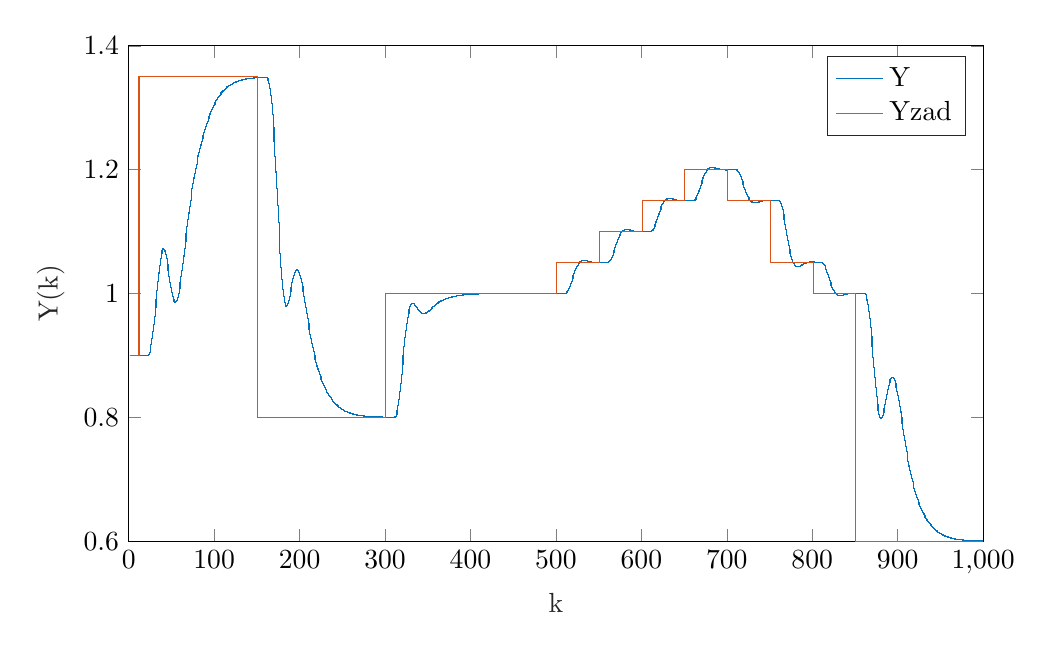
\begin{tikzpicture}

\begin{axis}[%
width=4.272in,
height=2.477in,
at={(0.717in,0.437in)},
scale only axis,
xmin=0,
xmax=1000,
xlabel style={font=\color{white!15!black}},
xlabel={k},
ymin=0.6,
ymax=1.4,
ylabel style={font=\color{white!15!black}},
ylabel={Y(k)},
axis background/.style={fill=white},
legend style={legend cell align=left, align=left, draw=white!15!black}
]
\addplot[const plot, color=mycolor1] table[row sep=crcr] {%
1	0.9\\
2	0.9\\
3	0.9\\
4	0.9\\
5	0.9\\
6	0.9\\
7	0.9\\
8	0.9\\
9	0.9\\
10	0.9\\
11	0.9\\
12	0.9\\
13	0.9\\
14	0.9\\
15	0.9\\
16	0.9\\
17	0.9\\
18	0.9\\
19	0.9\\
20	0.9\\
21	0.9\\
22	0.9003968325\\
23	0.90189871965075\\
24	0.905097390930944\\
25	0.91048229419639\\
26	0.918056433224468\\
27	0.927433096600071\\
28	0.938273783665903\\
29	0.950282922364603\\
30	0.963203128431219\\
31	0.976810952638584\\
32	0.990913067909024\\
33	1.00528631514411\\
34	1.01954237758236\\
35	1.0331213069164\\
36	1.04540993167318\\
37	1.05583128070471\\
38	1.06390928234672\\
39	1.06931097159114\\
40	1.07186911025769\\
41	1.07158847922252\\
42	1.06863804397751\\
43	1.06333012340567\\
44	1.05608954913757\\
45	1.04741780497607\\
46	1.03785662036586\\
47	1.02795412810544\\
48	1.01823558503116\\
49	1.00917976864102\\
50	1.00120147635191\\
51	0.994640041577812\\
52	0.989753417111267\\
53	0.986717137499602\\
54	0.985627335758079\\
55	0.986506935094653\\
56	0.989314144528384\\
57	0.99395244167742\\
58	1.0002813120917\\
59	1.00807544420228\\
60	1.01706199005888\\
61	1.02699920784427\\
62	1.0376766205516\\
63	1.04890620082479\\
64	1.06051201428843\\
65	1.07232901210076\\
66	1.08420684339106\\
67	1.09601243018348\\
68	1.10763143517995\\
69	1.11896901109357\\
70	1.12995022216284\\
71	1.14051996794932\\
72	1.15064208011019\\
73	1.1602975686262\\
74	1.16948222922669\\
75	1.17820391284457\\
76	1.18647971876071\\
77	1.19433330184344\\
78	1.20179242440633\\
79	1.20888683387355\\
80	1.21564650776663\\
81	1.22210027656174\\
82	1.22827481172225\\
83	1.23419394968074\\
84	1.23987831172611\\
85	1.24534517367498\\
86	1.25060853695477\\
87	1.25567935344909\\
88	1.2605658593891\\
89	1.26527397804291\\
90	1.26980775637859\\
91	1.27416980677365\\
92	1.27836173082388\\
93	1.28238450806516\\
94	1.28623883774239\\
95	1.28992542648755\\
96	1.29344521881577\\
97	1.29679957067556\\
98	1.29999036890309\\
99	1.30302010135791\\
100	1.30589188381876\\
101	1.308609450476\\
102	1.31117711514733\\
103	1.31359971025253\\
104	1.31588251019515\\
105	1.31803114519402\\
106	1.32005151085706\\
107	1.32194967795892\\
108	1.32373180602209\\
109	1.32540406345737\\
110	1.32697255622817\\
111	1.32844326628433\\
112	1.32982200038192\\
113	1.33111434937422\\
114	1.33232565762958\\
115	1.33346100190055\\
116	1.33452517873153\\
117	1.33552269933837\\
118	1.33645779081384\\
119	1.33733440249538\\
120	1.33815621636405\\
121	1.33892666041538\\
122	1.33964892404191\\
123	1.34032597458501\\
124	1.34096057434049\\
125	1.34155529743244\\
126	1.34211254609541\\
127	1.34263456602371\\
128	1.34312346055345\\
129	1.3435812035371\\
130	1.34400965084963\\
131	1.34441055053069\\
132	1.34478555161768\\
133	1.34513621176247\\
134	1.34546400374966\\
135	1.34577032104951\\
136	1.34605648254456\\
137	1.34632373656783\\
138	1.34657326438397\\
139	1.3468061832335\\
140	1.34702354904686\\
141	1.34722635892005\\
142	1.34741555342732\\
143	1.34759201883165\\
144	1.34775658923843\\
145	1.34791004872511\\
146	1.34805313346739\\
147	1.34818653387307\\
148	1.34831089672649\\
149	1.34842682734004\\
150	1.34853489170506\\
151	1.34863561863105\\
152	1.34872950186056\\
153	1.34881700214649\\
154	1.34889854927885\\
155	1.34897454404901\\
156	1.34904536014107\\
157	1.34911134594168\\
158	1.34917282626175\\
159	1.34923010396542\\
160	1.34928346150393\\
161	1.34893633030843\\
162	1.347480735028\\
163	1.34432517667354\\
164	1.33898042261346\\
165	1.33104683751027\\
166	1.32020309820478\\
167	1.30619615095281\\
168	1.28893934010788\\
169	1.2687712047618\\
170	1.24627062061622\\
171	1.22194195474919\\
172	1.19622334924821\\
173	1.16949414886195\\
174	1.14222434222232\\
175	1.11508828413476\\
176	1.08887334582708\\
177	1.06435015934846\\
178	1.04218636993476\\
179	1.02293137149171\\
180	1.00701910170842\\
181	0.994721322904822\\
182	0.986110682602668\\
183	0.981073278119624\\
184	0.979317125102481\\
185	0.980412958125832\\
186	0.98386126668566\\
187	0.989122397852625\\
188	0.995637106641996\\
189	1.00285677694917\\
190	1.01026811256633\\
191	1.01741191747306\\
192	1.02389604396558\\
193	1.0294029176117\\
194	1.03369234414385\\
195	1.0366004363147\\
196	1.03803534391325\\
197	1.03797041956529\\
198	1.03643558431708\\
199	1.03350766026712\\
200	1.02930032601268\\
201	1.02395423088642\\
202	1.01762768593651\\
203	1.01048823742095\\
204	1.00270532612858\\
205	0.994444145686068\\
206	0.985860736611826\\
207	0.977098290747883\\
208	0.96828459310023\\
209	0.959530492826011\\
210	0.950929271481\\
211	0.942556764436001\\
212	0.934472087960883\\
213	0.926718828140809\\
214	0.919326556908988\\
215	0.912312553529238\\
216	0.905683625457479\\
217	0.899437939451206\\
218	0.893566791073497\\
219	0.888056257542314\\
220	0.882888694579351\\
221	0.878044052067087\\
222	0.873500995645037\\
223	0.86923783172288\\
224	0.865233241729376\\
225	0.861466837813326\\
226	0.857919556797798\\
227	0.854573912142526\\
228	0.85141412520455\\
229	0.848426157432445\\
230	0.845597664516563\\
231	0.842917892170542\\
232	0.840377531346443\\
233	0.837968548474671\\
234	0.835684003932869\\
235	0.833517869521598\\
236	0.831464853368137\\
237	0.829520238473735\\
238	0.827679739132288\\
239	0.82593937771518\\
240	0.824295382849744\\
241	0.822744108827198\\
242	0.821281975151477\\
243	0.819905424465278\\
244	0.818610896639254\\
245	0.817394816555129\\
246	0.816253593022771\\
247	0.81518362631461\\
248	0.814181321948376\\
249	0.81324310857233\\
250	0.81236545807611\\
251	0.811544906343096\\
252	0.810778073361747\\
253	0.810061681708542\\
254	0.80939257269255\\
255	0.808767719703189\\
256	0.808184238522224\\
257	0.807639394545369\\
258	0.807130607007586\\
259	0.806655450420959\\
260	0.806211653516258\\
261	0.805797096032425\\
262	0.805409803725737\\
263	0.805047941976514\\
264	0.804709808359959\\
265	0.804393824523272\\
266	0.804098527677091\\
267	0.803822561969216\\
268	0.803564669965282\\
269	0.803323684417065\\
270	0.80309852045648\\
271	0.802888168313534\\
272	0.802691686620653\\
273	0.802508196334543\\
274	0.802336875280549\\
275	0.802176953303252\\
276	0.802027707990785\\
277	0.801888460928619\\
278	0.801758574430952\\
279	0.80163744869381\\
280	0.801524519312914\\
281	0.801419255110765\\
282	0.801321156220604\\
283	0.801229752379499\\
284	0.801144601388219\\
285	0.801065287701438\\
286	0.800991421117826\\
287	0.800922635545413\\
288	0.800858587823065\\
289	0.800798956583894\\
290	0.80074344115074\\
291	0.80069176045752\\
292	0.800643651993285\\
293	0.800598870768106\\
294	0.800557188301695\\
295	0.800518391636823\\
296	0.800482282380302\\
297	0.800448675774609\\
298	0.800417399803208\\
299	0.800388294332341\\
300	0.800361210291617\\
301	0.800336008895168\\
302	0.800312560904477\\
303	0.800290745933362\\
304	0.800270451794946\\
305	0.800251573889855\\
306	0.800234014634364\\
307	0.80021768292675\\
308	0.800202493649751\\
309	0.800188367206746\\
310	0.800175229089114\\
311	0.800559842732667\\
312	0.802050366462984\\
313	0.805238470319785\\
314	0.810613546808845\\
315	0.818507491991216\\
316	0.828791664694166\\
317	0.841030956060468\\
318	0.854788365265355\\
319	0.869560969689105\\
320	0.884805029864412\\
321	0.899989426769983\\
322	0.914632918444095\\
323	0.928327926581144\\
324	0.940753384105386\\
325	0.95167902731392\\
326	0.960964033860884\\
327	0.968552121748662\\
328	0.97446310672783\\
329	0.978781183407461\\
330	0.981641354558559\\
331	0.983215362833942\\
332	0.983698129117292\\
333	0.983295401034882\\
334	0.982213062348967\\
335	0.980648346626449\\
336	0.978783033574449\\
337	0.976778580757826\\
338	0.974773049984083\\
339	0.9728796247261\\
340	0.971186479095555\\
341	0.969757742505727\\
342	0.968635304293961\\
343	0.967841215263761\\
344	0.967380464802874\\
345	0.967243939826076\\
346	0.967411402633485\\
347	0.967854356686994\\
348	0.968538700420106\\
349	0.9694270981637\\
350	0.970481024226149\\
351	0.971662459609936\\
352	0.972935239704658\\
353	0.974266066434584\\
354	0.975625209768472\\
355	0.976986931472243\\
356	0.978329669034492\\
357	0.979636020219501\\
358	0.980892568845641\\
359	0.982089590692933\\
360	0.983220675528501\\
361	0.984282297402099\\
362	0.985273360962842\\
363	0.986194746885046\\
364	0.987048874816426\\
365	0.987839297775364\\
366	0.988570337776348\\
367	0.989246768758978\\
368	0.989873549701034\\
369	0.990455608139484\\
370	0.990997672205725\\
371	0.991504147680471\\
372	0.991979035450438\\
373	0.992425884051778\\
374	0.992847771654568\\
375	0.993247311816313\\
376	0.993626677548277\\
377	0.99398763863705\\
378	0.994331607690301\\
379	0.99465969098138\\
380	0.994972740810151\\
381	0.995271406742539\\
382	0.995556183710878\\
383	0.995827455530641\\
384	0.996085532901797\\
385	0.996330685406168\\
386	0.996563167381476\\
387	0.996783237851621\\
388	0.996991174915431\\
389	0.997187285151061\\
390	0.997371908695139\\
391	0.997545420706646\\
392	0.997708229933801\\
393	0.997860775078441\\
394	0.998003519604566\\
395	0.998136945571313\\
396	0.998261546992589\\
397	0.998377823141846\\
398	0.998486272135828\\
399	0.998587385049594\\
400	0.998681640739487\\
401	0.998769501483139\\
402	0.998851409487326\\
403	0.99892778426606\\
404	0.998999020852783\\
405	0.999065488781555\\
406	0.999127531751857\\
407	0.999185467879248\\
408	0.999239590428478\\
409	0.999290168925536\\
410	0.999337450549538\\
411	0.999381661712993\\
412	0.999423009749012\\
413	0.999461684635423\\
414	0.99949786069775\\
415	0.999531698245065\\
416	0.999563345104172\\
417	0.999592938028176\\
418	0.9996206039649\\
419	0.999646461178712\\
420	0.999670620226022\\
421	0.999693184790021\\
422	0.999714252384246\\
423	0.999733914937304\\
424	0.999752259272824\\
425	0.999769367499464\\
426	0.999785317325792\\
427	0.999800182314301\\
428	0.999814032087742\\
429	0.999826932499604\\
430	0.999838945779018\\
431	0.999850130658733\\
432	0.999860542493152\\
433	0.999870233371899\\
434	0.999879252232881\\
435	0.999887644977612\\
436	0.999895454590362\\
437	0.999902721261879\\
438	0.999909482517617\\
439	0.999915773349904\\
440	0.999921626353074\\
441	0.999927071860347\\
442	0.999932138081119\\
443	0.999936851237313\\
444	0.999941235697499\\
445	0.999945314107617\\
446	0.999949107517303\\
447	0.999952635501019\\
448	0.999955916273371\\
449	0.999958966798219\\
450	0.999961802891374\\
451	0.999964439316847\\
452	0.999966889876779\\
453	0.999969167495321\\
454	0.999971284296822\\
455	0.999973251678802\\
456	0.999975080380221\\
457	0.999976780545623\\
458	0.999978361785734\\
459	0.999979833235152\\
460	0.999981203607637\\
461	0.999982481249314\\
462	0.999983674189535\\
463	0.999984790188405\\
464	0.999985836779053\\
465	0.999986821301721\\
466	0.999987750925849\\
467	0.999988632655716\\
468	0.999989473314976\\
469	0.999990279505794\\
470	0.999991057539218\\
471	0.999991813335058\\
472	0.999992552291895\\
473	0.999993279130833\\
474	0.999993997720279\\
475	0.999994710893328\\
476	0.999995420274101\\
477	0.999996126134661\\
478	0.999996827309675\\
479	0.999997521196388\\
480	0.999998203857458\\
481	0.999998870229525\\
482	0.999999514426495\\
483	1.00000013011351\\
484	1.00000071091818\\
485	1.00000125084261\\
486	1.00000174464237\\
487	1.00000218735159\\
488	1.00000257340124\\
489	1.00000289634628\\
490	1.00000314898243\\
491	1.00000332379184\\
492	1.00000341386643\\
493	1.00000341414663\\
494	1.00000332255308\\
495	1.00000314077577\\
496	1.00000287462185\\
497	1.00000253391838\\
498	1.00000213202777\\
499	1.00000168506808\\
500	1.00000121094491\\
501	1.00000072830071\\
502	1.00000025547487\\
503	0.999999809549694\\
504	0.999999405539091\\
505	0.999999055760491\\
506	0.999998769412229\\
507	0.999998552361767\\
508	0.999998407134939\\
509	0.999998333084372\\
510	0.999998326706667\\
511	1.00022816400727\\
512	1.00102867263879\\
513	1.00256111853951\\
514	1.00485553365634\\
515	1.00785084371704\\
516	1.01142756606643\\
517	1.01543384445146\\
518	1.01970558556523\\
519	1.02408145406572\\
520	1.02841346479693\\
521	1.0325738815675\\
522	1.03645909130466\\
523	1.03999107206614\\
524	1.04311701532806\\
525	1.04580759958361\\
526	1.0480543460725\\
527	1.049866420781\\
528	1.05126718181537\\
529	1.05229070962995\\
530	1.05297850077517\\
531	1.05337645482387\\
532	1.05353223956612\\
533	1.0534930817239\\
534	1.05330399932406\\
535	1.05300646723258\\
536	1.05263748875684\\
537	1.05222903308764\\
538	1.05180779001019\\
539	1.05139518904769\\
540	1.05100762928565\\
541	1.05065686785433\\
542	1.05035051875677\\
543	1.05009261882204\\
544	1.04988422350663\\
545	1.04972400161414\\
546	1.04960880438403\\
547	1.04953419052564\\
548	1.04949489442631\\
549	1.04948522979565\\
550	1.04949942533005\\
551	1.04953189255484\\
552	1.04957742882714\\
553	1.04963136059437\\
554	1.0496896334601\\
555	1.04974885648416\\
556	1.04980630852147\\
557	1.0498599143719\\
558	1.04990819815825\\
559	1.04995022075361\\
560	1.04998550731941\\
561	1.05024375209137\\
562	1.05106601248049\\
563	1.05261402066359\\
564	1.05491844184168\\
565	1.05791893994075\\
566	1.06149682188186\\
567	1.06550102781917\\
568	1.06976823217528\\
569	1.07413781181701\\
570	1.07846241943362\\
571	1.08261487060331\\
572	1.08649201237328\\
573	1.09001619078861\\
574	1.09313487674184\\
575	1.09581894617813\\
576	1.09806004455502\\
577	1.09986739887789\\
578	1.10126437571079\\
579	1.10228502206223\\
580	1.10297076935095\\
581	1.10336742976465\\
582	1.10352256986276\\
583	1.10348330852939\\
584	1.10329455535014\\
585	1.10299768091755\\
586	1.10262959202597\\
587	1.10222217162277\\
588	1.10180203506547\\
589	1.10139054998219\\
590	1.1010040661256\\
591	1.10065430333978\\
592	1.10034884946362\\
593	1.10009172507545\\
594	1.09988397791337\\
595	1.09972427613677\\
596	1.09960947595878\\
597	1.09953514528782\\
598	1.09949603065394\\
599	1.09948645971353\\
600	1.09950067593592\\
601	1.09953310563732\\
602	1.09957856034431\\
603	1.09963237957394\\
604	1.09969052056886\\
605	1.09974960239765\\
606	1.09980691220596\\
607	1.09986038137095\\
608	1.09990853895652\\
609	1.09995044927212\\
610	1.09998563957929\\
611	1.10024380506812\\
612	1.10106600315813\\
613	1.10261396528716\\
614	1.10491835535872\\
615	1.10791883561593\\
616	1.11149671106498\\
617	1.11550091984421\\
618	1.11976813436729\\
619	1.12413772958385\\
620	1.12846235642068\\
621	1.13261482889136\\
622	1.13649199270175\\
623	1.14001619278939\\
624	1.14313489917126\\
625	1.14581898713748\\
626	1.14806010169256\\
627	1.14986746956747\\
628	1.15126445720437\\
629	1.15228511161516\\
630	1.15297086432041\\
631	1.15336752768264\\
632	1.15352266848589\\
633	1.15348340586828\\
634	1.15329464968149\\
635	1.15299777078204\\
636	1.15262967621529\\
637	1.15222224915862\\
638	1.15180210517331\\
639	1.15139061206215\\
640	1.15100411972267\\
641	1.15065434811485\\
642	1.15034888516675\\
643	1.15009175152245\\
644	1.14988399496629\\
645	1.1497242836888\\
646	1.14960947392375\\
647	1.14953513359438\\
648	1.14949600924429\\
649	1.14948642854654\\
650	1.14950063499442\\
651	1.14953305493934\\
652	1.14957849995795\\
653	1.14963230963564\\
654	1.14969044130506\\
655	1.14974951414958\\
656	1.14980681545755\\
657	1.14986027678001\\
658	1.14990842738917\\
659	1.14995033184088\\
660	1.14998551768495\\
661	1.15024368044565\\
662	1.15106587792651\\
663	1.15261384200238\\
664	1.15491823706823\\
665	1.15791872591184\\
666	1.16149661413177\\
667	1.16550084049556\\
668	1.16976807806529\\
669	1.17413770243305\\
670	1.17846236512896\\
671	1.18261488068981\\
672	1.18649209521689\\
673	1.19001635386304\\
674	1.19313512662672\\
675	1.19581928849498\\
676	1.19806048384307\\
677	1.19986793842108\\
678	1.20126501733827\\
679	1.20228576595377\\
680	1.20297161388019\\
681	1.20336837140807\\
682	1.20352360319298\\
683	1.20348442630113\\
684	1.20329574867717\\
685	1.20299893953046\\
686	1.20263090459444\\
687	1.20222352566238\\
688	1.20180341635585\\
689	1.20139194205226\\
690	1.20100545008479\\
691	1.20065565814451\\
692	1.20035015258685\\
693	1.20009295347811\\
694	1.19988510918585\\
695	1.19972528967548\\
696	1.1996103540575\\
697	1.19953587404861\\
698	1.19949660065243\\
699	1.19948686638356\\
700	1.19950091966657\\
701	1.19953319159886\\
702	1.19957849807756\\
703	1.19963218239031\\
704	1.19969020481511\\
705	1.19974918664166\\
706	1.19980641639773\\
707	1.19985982602786\\
708	1.19990794441452\\
709	1.19994983503547\\
710	1.19998502379229\\
711	1.19978364025359\\
712	1.19900506883166\\
713	1.19748848852092\\
714	1.19520447712479\\
715	1.19221482274493\\
716	1.1886397735737\\
717	1.18463195957753\\
718	1.1803562212542\\
719	1.17597458836355\\
720	1.17163566923903\\
721	1.1674677404672\\
722	1.1635748671452\\
723	1.160035434213\\
724	1.1569025274281\\
725	1.15420566598218\\
726	1.15195345505438\\
727	1.15013679337815\\
728	1.14873233604963\\
729	1.14770597454426\\
730	1.14701615283382\\
731	1.14661688960787\\
732	1.14646042126997\\
733	1.14649941830696\\
734	1.14668875882035\\
735	1.1469868677092\\
736	1.1473566486424\\
737	1.14776604867571\\
738	1.14818830460497\\
739	1.14860192464769\\
740	1.14899045906282\\
741	1.14934211167655\\
742	1.14964924063422\\
743	1.14990779164877\\
744	1.1501167010979\\
745	1.15027729998753\\
746	1.15039274342041\\
747	1.15046748407847\\
748	1.15050680256423\\
749	1.15051640240073\\
750	1.15050207315234\\
751	1.1504694215411\\
752	1.1504236675935\\
753	1.15036950072848\\
754	1.15031098923014\\
755	1.15025153566516\\
756	1.15019387042108\\
757	1.15014007556994\\
758	1.1500916316146\\
759	1.15004948027031\\
760	1.15001409719536\\
761	1.14958833731199\\
762	1.14812043083609\\
763	1.14523865942341\\
764	1.14084671380022\\
765	1.13504127673259\\
766	1.12804466615991\\
767	1.12015100333421\\
768	1.11168437574727\\
769	1.10296747958275\\
770	1.09429926002391\\
771	1.08594012361467\\
772	1.07810337504623\\
773	1.07095162881365\\
774	1.06459706022071\\
775	1.05910448549191\\
776	1.05449639233327\\
777	1.05075917541719\\
778	1.04784996166999\\
779	1.04570353428551\\
780	1.04423897919365\\
781	1.04336578117756\\
782	1.0429891876047\\
783	1.04301473514266\\
784	1.04335189879907\\
785	1.0439168735867\\
786	1.04463453789366\\
787	1.04543967489127\\
788	1.04627754714129\\
789	1.04710392940936\\
790	1.0478847065174\\
791	1.04859514041398\\
792	1.04921890383235\\
793	1.04974696816092\\
794	1.05017642154723\\
795	1.05050928071592\\
796	1.05075134726344\\
797	1.05091114690039\\
798	1.05099897869918\\
799	1.0510260911862\\
800	1.05100399329118\\
801	1.05094390082363\\
802	1.05085631329618\\
803	1.05075071149879\\
804	1.05063536313641\\
805	1.05051722193368\\
806	1.05040190471764\\
807	1.05029373094059\\
808	1.05019580972577\\
809	1.05011016064176\\
810	1.05003785588558\\
811	1.04974939130754\\
812	1.04890356966723\\
813	1.04733826429604\\
814	1.04502223119779\\
815	1.04201510682128\\
816	1.03843481910168\\
817	1.03443164371394\\
818	1.0301681405683\\
819	1.0258042144772\\
820	1.02148656251984\\
821	1.01734180043004\\
822	1.01347260113609\\
823	1.00995622904285\\
824	1.00684491172281\\
825	1.00416755398639\\
826	1.00193236536802\\
827	1.00013003854915\\
828	0.998737181050486\\
829	0.997719763905788\\
830	0.997036407597764\\
831	0.99664137630628\\
832	0.996487195870941\\
833	0.996526848518225\\
834	0.996715528353883\\
835	0.997011966123078\\
836	0.997379350231737\\
837	0.997785883616523\\
838	0.998205025209417\\
839	0.998615469201089\\
840	0.99900091529966\\
841	0.999349681537251\\
842	0.999654207544668\\
843	0.999910491195493\\
844	1.00011749564224\\
845	1.0002765574786\\
846	1.00039082043127\\
847	1.00046471290338\\
848	1.000503482074\\
849	1.00051279225551\\
850	1.000498390911\\
851	1.00046584217858\\
852	1.00042032493703\\
853	1.0003664903436\\
854	1.0003083723239\\
855	1.00024934362097\\
856	1.0001921096335\\
857	1.00013873230425\\
858	1.00009067667262\\
859	1.00004887329793\\
860	1.00001379051652\\
861	0.999588283632366\\
862	0.998063323913407\\
863	0.994846464064819\\
864	0.98944761805966\\
865	0.981533712720184\\
866	0.971232399994249\\
867	0.958978462724507\\
868	0.945152006601503\\
869	0.930084475107254\\
870	0.91406404658818\\
871	0.89735950256567\\
872	0.88036353112354\\
873	0.863642151677558\\
874	0.847821914249622\\
875	0.833508089805453\\
876	0.821226850525233\\
877	0.811384992419135\\
878	0.804244399817666\\
879	0.799910040481478\\
880	0.798330666423155\\
881	0.799312147471207\\
882	0.802541494293916\\
883	0.80761718186021\\
884	0.814081452252363\\
885	0.821451496659083\\
886	0.829247426022146\\
887	0.837015758478065\\
888	0.844347797581872\\
889	0.850892770277009\\
890	0.856365957972088\\
891	0.860552305133297\\
892	0.863306147068478\\
893	0.864547779522748\\
894	0.864257613424378\\
895	0.862468633150282\\
896	0.859257818863412\\
897	0.854737113886461\\
898	0.849044426026987\\
899	0.842335054852109\\
900	0.834773841102287\\
901	0.826528244225047\\
902	0.817762472566864\\
903	0.808632720099115\\
904	0.799283504714702\\
905	0.789845056365349\\
906	0.7804316682437\\
907	0.77114090001364\\
908	0.762053507600367\\
909	0.753233967915598\\
910	0.744731467668037\\
911	0.736581231644002\\
912	0.728806076147477\\
913	0.721418086382395\\
914	0.714420331305964\\
915	0.707808544907449\\
916	0.701572718171211\\
917	0.69569856053645\\
918	0.690168803002326\\
919	0.684964326828106\\
920	0.680065111857996\\
921	0.675451006785497\\
922	0.671102330181021\\
923	0.66700031592938\\
924	0.663127420004363\\
925	0.659467507425215\\
926	0.656005938994835\\
927	0.652729577219829\\
928	0.649626729863566\\
929	0.646687048085095\\
930	0.64390139425089\\
931	0.641261692421392\\
932	0.638760772335961\\
933	0.636392215558168\\
934	0.634150210385393\\
935	0.632029420236898\\
936	0.630024868556797\\
937	0.628131842619001\\
938	0.626345816055157\\
939	0.624662388368043\\
940	0.623077240486323\\
941	0.621586105013042\\
942	0.620184749367949\\
943	0.618868969765027\\
944	0.617634593868367\\
945	0.616477489999134\\
946	0.615393580895217\\
947	0.614378860221947\\
948	0.613429410270978\\
949	0.612541419547111\\
950	0.611711199212292\\
951	0.61093519761797\\
952	0.610210012400805\\
953	0.609532399834827\\
954	0.608899281320934\\
955	0.608307747049758\\
956	0.607755056996233\\
957	0.60723863949486\\
958	0.60675608770619\\
959	0.606305154320546\\
960	0.605883744858377\\
961	0.605489909921705\\
962	0.605121836732021\\
963	0.604777840260295\\
964	0.604456354217985\\
965	0.60415592213704\\
966	0.603875188724434\\
967	0.603612891634935\\
968	0.603367853766113\\
969	0.603138976143343\\
970	0.602925231430493\\
971	0.602725658074575\\
972	0.602539355070055\\
973	0.602365477310614\\
974	0.602203231482763\\
975	0.602051872446291\\
976	0.601910700040706\\
977	0.601779056253982\\
978	0.601656322689535\\
979	0.601541918272017\\
980	0.601435297143726\\
981	0.601335946715619\\
982	0.601243385846271\\
983	0.601157163129073\\
984	0.601076855273155\\
985	0.601002065567303\\
986	0.600932422418777\\
987	0.600867578420276\\
988	0.600807209531692\\
989	0.600751013744165\\
990	0.600698709501649\\
991	0.600650034069955\\
992	0.600604741976072\\
993	0.600562603588979\\
994	0.600523403874794\\
995	0.600486941331865\\
996	0.600453027093201\\
997	0.600421484172734\\
998	0.60039214682665\\
999	0.600364859999913\\
1000	0.600339478830002\\
};
\addlegendentry{Y}

\addplot[const plot, color=mycolor2] table[row sep=crcr] {%
1	0.9\\
2	0.9\\
3	0.9\\
4	0.9\\
5	0.9\\
6	0.9\\
7	0.9\\
8	0.9\\
9	0.9\\
10	0.9\\
11	0.9\\
12	1.35\\
13	1.35\\
14	1.35\\
15	1.35\\
16	1.35\\
17	1.35\\
18	1.35\\
19	1.35\\
20	1.35\\
21	1.35\\
22	1.35\\
23	1.35\\
24	1.35\\
25	1.35\\
26	1.35\\
27	1.35\\
28	1.35\\
29	1.35\\
30	1.35\\
31	1.35\\
32	1.35\\
33	1.35\\
34	1.35\\
35	1.35\\
36	1.35\\
37	1.35\\
38	1.35\\
39	1.35\\
40	1.35\\
41	1.35\\
42	1.35\\
43	1.35\\
44	1.35\\
45	1.35\\
46	1.35\\
47	1.35\\
48	1.35\\
49	1.35\\
50	1.35\\
51	1.35\\
52	1.35\\
53	1.35\\
54	1.35\\
55	1.35\\
56	1.35\\
57	1.35\\
58	1.35\\
59	1.35\\
60	1.35\\
61	1.35\\
62	1.35\\
63	1.35\\
64	1.35\\
65	1.35\\
66	1.35\\
67	1.35\\
68	1.35\\
69	1.35\\
70	1.35\\
71	1.35\\
72	1.35\\
73	1.35\\
74	1.35\\
75	1.35\\
76	1.35\\
77	1.35\\
78	1.35\\
79	1.35\\
80	1.35\\
81	1.35\\
82	1.35\\
83	1.35\\
84	1.35\\
85	1.35\\
86	1.35\\
87	1.35\\
88	1.35\\
89	1.35\\
90	1.35\\
91	1.35\\
92	1.35\\
93	1.35\\
94	1.35\\
95	1.35\\
96	1.35\\
97	1.35\\
98	1.35\\
99	1.35\\
100	1.35\\
101	1.35\\
102	1.35\\
103	1.35\\
104	1.35\\
105	1.35\\
106	1.35\\
107	1.35\\
108	1.35\\
109	1.35\\
110	1.35\\
111	1.35\\
112	1.35\\
113	1.35\\
114	1.35\\
115	1.35\\
116	1.35\\
117	1.35\\
118	1.35\\
119	1.35\\
120	1.35\\
121	1.35\\
122	1.35\\
123	1.35\\
124	1.35\\
125	1.35\\
126	1.35\\
127	1.35\\
128	1.35\\
129	1.35\\
130	1.35\\
131	1.35\\
132	1.35\\
133	1.35\\
134	1.35\\
135	1.35\\
136	1.35\\
137	1.35\\
138	1.35\\
139	1.35\\
140	1.35\\
141	1.35\\
142	1.35\\
143	1.35\\
144	1.35\\
145	1.35\\
146	1.35\\
147	1.35\\
148	1.35\\
149	1.35\\
150	1.35\\
151	0.8\\
152	0.8\\
153	0.8\\
154	0.8\\
155	0.8\\
156	0.8\\
157	0.8\\
158	0.8\\
159	0.8\\
160	0.8\\
161	0.8\\
162	0.8\\
163	0.8\\
164	0.8\\
165	0.8\\
166	0.8\\
167	0.8\\
168	0.8\\
169	0.8\\
170	0.8\\
171	0.8\\
172	0.8\\
173	0.8\\
174	0.8\\
175	0.8\\
176	0.8\\
177	0.8\\
178	0.8\\
179	0.8\\
180	0.8\\
181	0.8\\
182	0.8\\
183	0.8\\
184	0.8\\
185	0.8\\
186	0.8\\
187	0.8\\
188	0.8\\
189	0.8\\
190	0.8\\
191	0.8\\
192	0.8\\
193	0.8\\
194	0.8\\
195	0.8\\
196	0.8\\
197	0.8\\
198	0.8\\
199	0.8\\
200	0.8\\
201	0.8\\
202	0.8\\
203	0.8\\
204	0.8\\
205	0.8\\
206	0.8\\
207	0.8\\
208	0.8\\
209	0.8\\
210	0.8\\
211	0.8\\
212	0.8\\
213	0.8\\
214	0.8\\
215	0.8\\
216	0.8\\
217	0.8\\
218	0.8\\
219	0.8\\
220	0.8\\
221	0.8\\
222	0.8\\
223	0.8\\
224	0.8\\
225	0.8\\
226	0.8\\
227	0.8\\
228	0.8\\
229	0.8\\
230	0.8\\
231	0.8\\
232	0.8\\
233	0.8\\
234	0.8\\
235	0.8\\
236	0.8\\
237	0.8\\
238	0.8\\
239	0.8\\
240	0.8\\
241	0.8\\
242	0.8\\
243	0.8\\
244	0.8\\
245	0.8\\
246	0.8\\
247	0.8\\
248	0.8\\
249	0.8\\
250	0.8\\
251	0.8\\
252	0.8\\
253	0.8\\
254	0.8\\
255	0.8\\
256	0.8\\
257	0.8\\
258	0.8\\
259	0.8\\
260	0.8\\
261	0.8\\
262	0.8\\
263	0.8\\
264	0.8\\
265	0.8\\
266	0.8\\
267	0.8\\
268	0.8\\
269	0.8\\
270	0.8\\
271	0.8\\
272	0.8\\
273	0.8\\
274	0.8\\
275	0.8\\
276	0.8\\
277	0.8\\
278	0.8\\
279	0.8\\
280	0.8\\
281	0.8\\
282	0.8\\
283	0.8\\
284	0.8\\
285	0.8\\
286	0.8\\
287	0.8\\
288	0.8\\
289	0.8\\
290	0.8\\
291	0.8\\
292	0.8\\
293	0.8\\
294	0.8\\
295	0.8\\
296	0.8\\
297	0.8\\
298	0.8\\
299	0.8\\
300	0.8\\
301	1\\
302	1\\
303	1\\
304	1\\
305	1\\
306	1\\
307	1\\
308	1\\
309	1\\
310	1\\
311	1\\
312	1\\
313	1\\
314	1\\
315	1\\
316	1\\
317	1\\
318	1\\
319	1\\
320	1\\
321	1\\
322	1\\
323	1\\
324	1\\
325	1\\
326	1\\
327	1\\
328	1\\
329	1\\
330	1\\
331	1\\
332	1\\
333	1\\
334	1\\
335	1\\
336	1\\
337	1\\
338	1\\
339	1\\
340	1\\
341	1\\
342	1\\
343	1\\
344	1\\
345	1\\
346	1\\
347	1\\
348	1\\
349	1\\
350	1\\
351	1\\
352	1\\
353	1\\
354	1\\
355	1\\
356	1\\
357	1\\
358	1\\
359	1\\
360	1\\
361	1\\
362	1\\
363	1\\
364	1\\
365	1\\
366	1\\
367	1\\
368	1\\
369	1\\
370	1\\
371	1\\
372	1\\
373	1\\
374	1\\
375	1\\
376	1\\
377	1\\
378	1\\
379	1\\
380	1\\
381	1\\
382	1\\
383	1\\
384	1\\
385	1\\
386	1\\
387	1\\
388	1\\
389	1\\
390	1\\
391	1\\
392	1\\
393	1\\
394	1\\
395	1\\
396	1\\
397	1\\
398	1\\
399	1\\
400	1\\
401	1\\
402	1\\
403	1\\
404	1\\
405	1\\
406	1\\
407	1\\
408	1\\
409	1\\
410	1\\
411	1\\
412	1\\
413	1\\
414	1\\
415	1\\
416	1\\
417	1\\
418	1\\
419	1\\
420	1\\
421	1\\
422	1\\
423	1\\
424	1\\
425	1\\
426	1\\
427	1\\
428	1\\
429	1\\
430	1\\
431	1\\
432	1\\
433	1\\
434	1\\
435	1\\
436	1\\
437	1\\
438	1\\
439	1\\
440	1\\
441	1\\
442	1\\
443	1\\
444	1\\
445	1\\
446	1\\
447	1\\
448	1\\
449	1\\
450	1\\
451	1\\
452	1\\
453	1\\
454	1\\
455	1\\
456	1\\
457	1\\
458	1\\
459	1\\
460	1\\
461	1\\
462	1\\
463	1\\
464	1\\
465	1\\
466	1\\
467	1\\
468	1\\
469	1\\
470	1\\
471	1\\
472	1\\
473	1\\
474	1\\
475	1\\
476	1\\
477	1\\
478	1\\
479	1\\
480	1\\
481	1\\
482	1\\
483	1\\
484	1\\
485	1\\
486	1\\
487	1\\
488	1\\
489	1\\
490	1\\
491	1\\
492	1\\
493	1\\
494	1\\
495	1\\
496	1\\
497	1\\
498	1\\
499	1\\
500	1\\
501	1.05\\
502	1.05\\
503	1.05\\
504	1.05\\
505	1.05\\
506	1.05\\
507	1.05\\
508	1.05\\
509	1.05\\
510	1.05\\
511	1.05\\
512	1.05\\
513	1.05\\
514	1.05\\
515	1.05\\
516	1.05\\
517	1.05\\
518	1.05\\
519	1.05\\
520	1.05\\
521	1.05\\
522	1.05\\
523	1.05\\
524	1.05\\
525	1.05\\
526	1.05\\
527	1.05\\
528	1.05\\
529	1.05\\
530	1.05\\
531	1.05\\
532	1.05\\
533	1.05\\
534	1.05\\
535	1.05\\
536	1.05\\
537	1.05\\
538	1.05\\
539	1.05\\
540	1.05\\
541	1.05\\
542	1.05\\
543	1.05\\
544	1.05\\
545	1.05\\
546	1.05\\
547	1.05\\
548	1.05\\
549	1.05\\
550	1.05\\
551	1.1\\
552	1.1\\
553	1.1\\
554	1.1\\
555	1.1\\
556	1.1\\
557	1.1\\
558	1.1\\
559	1.1\\
560	1.1\\
561	1.1\\
562	1.1\\
563	1.1\\
564	1.1\\
565	1.1\\
566	1.1\\
567	1.1\\
568	1.1\\
569	1.1\\
570	1.1\\
571	1.1\\
572	1.1\\
573	1.1\\
574	1.1\\
575	1.1\\
576	1.1\\
577	1.1\\
578	1.1\\
579	1.1\\
580	1.1\\
581	1.1\\
582	1.1\\
583	1.1\\
584	1.1\\
585	1.1\\
586	1.1\\
587	1.1\\
588	1.1\\
589	1.1\\
590	1.1\\
591	1.1\\
592	1.1\\
593	1.1\\
594	1.1\\
595	1.1\\
596	1.1\\
597	1.1\\
598	1.1\\
599	1.1\\
600	1.1\\
601	1.15\\
602	1.15\\
603	1.15\\
604	1.15\\
605	1.15\\
606	1.15\\
607	1.15\\
608	1.15\\
609	1.15\\
610	1.15\\
611	1.15\\
612	1.15\\
613	1.15\\
614	1.15\\
615	1.15\\
616	1.15\\
617	1.15\\
618	1.15\\
619	1.15\\
620	1.15\\
621	1.15\\
622	1.15\\
623	1.15\\
624	1.15\\
625	1.15\\
626	1.15\\
627	1.15\\
628	1.15\\
629	1.15\\
630	1.15\\
631	1.15\\
632	1.15\\
633	1.15\\
634	1.15\\
635	1.15\\
636	1.15\\
637	1.15\\
638	1.15\\
639	1.15\\
640	1.15\\
641	1.15\\
642	1.15\\
643	1.15\\
644	1.15\\
645	1.15\\
646	1.15\\
647	1.15\\
648	1.15\\
649	1.15\\
650	1.15\\
651	1.2\\
652	1.2\\
653	1.2\\
654	1.2\\
655	1.2\\
656	1.2\\
657	1.2\\
658	1.2\\
659	1.2\\
660	1.2\\
661	1.2\\
662	1.2\\
663	1.2\\
664	1.2\\
665	1.2\\
666	1.2\\
667	1.2\\
668	1.2\\
669	1.2\\
670	1.2\\
671	1.2\\
672	1.2\\
673	1.2\\
674	1.2\\
675	1.2\\
676	1.2\\
677	1.2\\
678	1.2\\
679	1.2\\
680	1.2\\
681	1.2\\
682	1.2\\
683	1.2\\
684	1.2\\
685	1.2\\
686	1.2\\
687	1.2\\
688	1.2\\
689	1.2\\
690	1.2\\
691	1.2\\
692	1.2\\
693	1.2\\
694	1.2\\
695	1.2\\
696	1.2\\
697	1.2\\
698	1.2\\
699	1.2\\
700	1.2\\
701	1.15\\
702	1.15\\
703	1.15\\
704	1.15\\
705	1.15\\
706	1.15\\
707	1.15\\
708	1.15\\
709	1.15\\
710	1.15\\
711	1.15\\
712	1.15\\
713	1.15\\
714	1.15\\
715	1.15\\
716	1.15\\
717	1.15\\
718	1.15\\
719	1.15\\
720	1.15\\
721	1.15\\
722	1.15\\
723	1.15\\
724	1.15\\
725	1.15\\
726	1.15\\
727	1.15\\
728	1.15\\
729	1.15\\
730	1.15\\
731	1.15\\
732	1.15\\
733	1.15\\
734	1.15\\
735	1.15\\
736	1.15\\
737	1.15\\
738	1.15\\
739	1.15\\
740	1.15\\
741	1.15\\
742	1.15\\
743	1.15\\
744	1.15\\
745	1.15\\
746	1.15\\
747	1.15\\
748	1.15\\
749	1.15\\
750	1.15\\
751	1.05\\
752	1.05\\
753	1.05\\
754	1.05\\
755	1.05\\
756	1.05\\
757	1.05\\
758	1.05\\
759	1.05\\
760	1.05\\
761	1.05\\
762	1.05\\
763	1.05\\
764	1.05\\
765	1.05\\
766	1.05\\
767	1.05\\
768	1.05\\
769	1.05\\
770	1.05\\
771	1.05\\
772	1.05\\
773	1.05\\
774	1.05\\
775	1.05\\
776	1.05\\
777	1.05\\
778	1.05\\
779	1.05\\
780	1.05\\
781	1.05\\
782	1.05\\
783	1.05\\
784	1.05\\
785	1.05\\
786	1.05\\
787	1.05\\
788	1.05\\
789	1.05\\
790	1.05\\
791	1.05\\
792	1.05\\
793	1.05\\
794	1.05\\
795	1.05\\
796	1.05\\
797	1.05\\
798	1.05\\
799	1.05\\
800	1.05\\
801	1\\
802	1\\
803	1\\
804	1\\
805	1\\
806	1\\
807	1\\
808	1\\
809	1\\
810	1\\
811	1\\
812	1\\
813	1\\
814	1\\
815	1\\
816	1\\
817	1\\
818	1\\
819	1\\
820	1\\
821	1\\
822	1\\
823	1\\
824	1\\
825	1\\
826	1\\
827	1\\
828	1\\
829	1\\
830	1\\
831	1\\
832	1\\
833	1\\
834	1\\
835	1\\
836	1\\
837	1\\
838	1\\
839	1\\
840	1\\
841	1\\
842	1\\
843	1\\
844	1\\
845	1\\
846	1\\
847	1\\
848	1\\
849	1\\
850	1\\
851	0.6\\
852	0.6\\
853	0.6\\
854	0.6\\
855	0.6\\
856	0.6\\
857	0.6\\
858	0.6\\
859	0.6\\
860	0.6\\
861	0.6\\
862	0.6\\
863	0.6\\
864	0.6\\
865	0.6\\
866	0.6\\
867	0.6\\
868	0.6\\
869	0.6\\
870	0.6\\
871	0.6\\
872	0.6\\
873	0.6\\
874	0.6\\
875	0.6\\
876	0.6\\
877	0.6\\
878	0.6\\
879	0.6\\
880	0.6\\
881	0.6\\
882	0.6\\
883	0.6\\
884	0.6\\
885	0.6\\
886	0.6\\
887	0.6\\
888	0.6\\
889	0.6\\
890	0.6\\
891	0.6\\
892	0.6\\
893	0.6\\
894	0.6\\
895	0.6\\
896	0.6\\
897	0.6\\
898	0.6\\
899	0.6\\
900	0.6\\
901	0.6\\
902	0.6\\
903	0.6\\
904	0.6\\
905	0.6\\
906	0.6\\
907	0.6\\
908	0.6\\
909	0.6\\
910	0.6\\
911	0.6\\
912	0.6\\
913	0.6\\
914	0.6\\
915	0.6\\
916	0.6\\
917	0.6\\
918	0.6\\
919	0.6\\
920	0.6\\
921	0.6\\
922	0.6\\
923	0.6\\
924	0.6\\
925	0.6\\
926	0.6\\
927	0.6\\
928	0.6\\
929	0.6\\
930	0.6\\
931	0.6\\
932	0.6\\
933	0.6\\
934	0.6\\
935	0.6\\
936	0.6\\
937	0.6\\
938	0.6\\
939	0.6\\
940	0.6\\
941	0.6\\
942	0.6\\
943	0.6\\
944	0.6\\
945	0.6\\
946	0.6\\
947	0.6\\
948	0.6\\
949	0.6\\
950	0.6\\
951	0.6\\
952	0.6\\
953	0.6\\
954	0.6\\
955	0.6\\
956	0.6\\
957	0.6\\
958	0.6\\
959	0.6\\
960	0.6\\
961	0.6\\
962	0.6\\
963	0.6\\
964	0.6\\
965	0.6\\
966	0.6\\
967	0.6\\
968	0.6\\
969	0.6\\
970	0.6\\
971	0.6\\
972	0.6\\
973	0.6\\
974	0.6\\
975	0.6\\
976	0.6\\
977	0.6\\
978	0.6\\
979	0.6\\
980	0.6\\
981	0.6\\
982	0.6\\
983	0.6\\
984	0.6\\
985	0.6\\
986	0.6\\
987	0.6\\
988	0.6\\
989	0.6\\
990	0.6\\
991	0.6\\
992	0.6\\
993	0.6\\
994	0.6\\
995	0.6\\
996	0.6\\
997	0.6\\
998	0.6\\
999	0.6\\
1000	0.6\\
};
\addlegendentry{Yzad}

\end{axis}
\end{tikzpicture}%
\caption{Wyjście DMC dla parametrów $N=100$, $N_u=10$, $\lambda=1$}
\end{figure}

\begin{equation}
E = 22,3271
\end{equation}

Zwiększjąc $\lambda$ do $50$ otrzymujemy dużo lepsze śledzenie na wyjściu.


\begin{figure}[H]
\centering
% This file was created by matlab2tikz.
%
%The latest updates can be retrieved from
%  http://www.mathworks.com/matlabcentral/fileexchange/22022-matlab2tikz-matlab2tikz
%where you can also make suggestions and rate matlab2tikz.
%
\definecolor{mycolor1}{rgb}{0.00000,0.44700,0.74100}%
%
\begin{tikzpicture}

\begin{axis}[%
width=4.272in,
height=2.477in,
at={(0.717in,0.437in)},
scale only axis,
xmin=0,
xmax=1000,
xlabel style={font=\color{white!15!black}},
xlabel={k},
ymin=2.5,
ymax=3.4,
ylabel style={font=\color{white!15!black}},
ylabel={U(k)},
axis background/.style={fill=white}
]
\addplot[const plot, color=mycolor1, forget plot] table[row sep=crcr] {%
1	3\\
2	3\\
3	3\\
4	3\\
5	3\\
6	3\\
7	3\\
8	3\\
9	3\\
10	3\\
11	3\\
12	3.05972415564318\\
13	3.11205906028104\\
14	3.15767008516089\\
15	3.19717680024687\\
16	3.23115582967668\\
17	3.26014338115051\\
18	3.28463751761913\\
19	3.3\\
20	3.3\\
21	3.3\\
22	3.3\\
23	3.3\\
24	3.3\\
25	3.3\\
26	3.3\\
27	3.3\\
28	3.2998834404784\\
29	3.2987491862097\\
30	3.29678785929052\\
31	3.29418777960509\\
32	3.2911270745116\\
33	3.2877683219256\\
34	3.28425521067832\\
35	3.28071078458183\\
36	3.27723690789211\\
37	3.27391465123569\\
38	3.27080543164979\\
39	3.26795331128189\\
40	3.26538785823509\\
41	3.26312663810647\\
42	3.26117737786248\\
43	3.25953983918826\\
44	3.25820743445863\\
45	3.25716861494082\\
46	3.25640805769515\\
47	3.25590767484013\\
48	3.25564746634992\\
49	3.25560623531929\\
50	3.2557621826304\\
51	3.25609339616247\\
52	3.25657824807325\\
53	3.25719571223204\\
54	3.25792561257861\\
55	3.25874881200651\\
56	3.25964735030828\\
57	3.26060453876329\\
58	3.26160501808575\\
59	3.2626347856707\\
60	3.26368119737375\\
61	3.26473294842596\\
62	3.2657800375148\\
63	3.26681371754795\\
64	3.26782643615521\\
65	3.26881176856849\\
66	3.26976434514907\\
67	3.27067977549861\\
68	3.27155457079411\\
69	3.27238606572353\\
70	3.27317234116432\\
71	3.27391214854082\\
72	3.27460483661354\\
73	3.27525028129395\\
74	3.27584881893848\\
75	3.2764011834541\\
76	3.27690844744315\\
77	3.2773719675254\\
78	3.27779333389864\\
79	3.27817432413505\\
80	3.27851686115662\\
81	3.27882297528922\\
82	3.27909477025888\\
83	3.27933439296616\\
84	3.27954400685269\\
85	3.2797257686583\\
86	3.27988180835621\\
87	3.28001421204767\\
88	3.2801250076023\\
89	3.28021615280448\\
90	3.28028952579787\\
91	3.28034691761491\\
92	3.28039002658464\\
93	3.28042045442078\\
94	3.28043970380134\\
95	3.2804491772609\\
96	3.28045017722795\\
97	3.28044390705025\\
98	3.28043147286282\\
99	3.28041388616415\\
100	3.28039206697764\\
101	3.28036684748582\\
102	3.28033897603598\\
103	3.2803091214255\\
104	3.28027787738545\\
105	3.28024576718975\\
106	3.28021324832645\\
107	3.28018071717534\\
108	3.28014851364421\\
109	3.28011692572266\\
110	3.28008619391936\\
111	3.28005651555414\\
112	3.28002804888204\\
113	3.28000091703124\\
114	3.27997521174109\\
115	3.27995099689066\\
116	3.27992831181135\\
117	3.27990717438054\\
118	3.27988758389558\\
119	3.2798695237301\\
120	3.2798529637761\\
121	3.27983786267741\\
122	3.27982416986126\\
123	3.2798118273756\\
124	3.27980077154114\\
125	3.27979093442738\\
126	3.27978224516233\\
127	3.27977463108644\\
128	3.27976801876061\\
129	3.27976233483891\\
130	3.27975750681628\\
131	3.27975346366102\\
132	3.27975013634226\\
133	3.2797474582617\\
134	3.27974536559878\\
135	3.2797437975782\\
136	3.27974269666783\\
137	3.27974200871507\\
138	3.27974168302886\\
139	3.2797416724143\\
140	3.27974193316622\\
141	3.27974242502754\\
142	3.27974311111798\\
143	3.27974395783793\\
144	3.27974493475203\\
145	3.27974601445654\\
146	3.27974717243417\\
147	3.27974838689955\\
148	3.27974963863829\\
149	3.27975091084222\\
150	3.27975218894289\\
151	3.20675727021479\\
152	3.14279364108695\\
153	3.08704806119708\\
154	3.0387632711203\\
155	2.99723450221502\\
156	2.96180638500209\\
157	2.93187017251837\\
158	2.90686121149235\\
159	2.88625660792808\\
160	2.869573045128\\
161	2.85636472166139\\
162	2.84622138457746\\
163	2.83876643951856\\
164	2.833655124525\\
165	2.83057273842602\\
166	2.8292329179443\\
167	2.82937596014433\\
168	2.83076718874991\\
169	2.83319536424808\\
170	2.836471138675\\
171	2.8404255566236\\
172	2.84490860438656\\
173	2.84978780930648\\
174	2.85494689139718\\
175	2.86028446916533\\
176	2.86571282133382\\
177	2.87115670587545\\
178	2.87655223742975\\
179	2.88184582381688\\
180	2.88699316197827\\
181	2.89195829330862\\
182	2.89671271800906\\
183	2.90123456775893\\
184	2.90550783569529\\
185	2.90952166241012\\
186	2.91326967642626\\
187	2.91674938739599\\
188	2.91996161183643\\
189	2.92290998985577\\
190	2.92560052319427\\
191	2.92804115758355\\
192	2.93024140703022\\
193	2.93221201759208\\
194	2.93396466820035\\
195	2.93551170608732\\
196	2.93686591440419\\
197	2.93804030965544\\
198	2.93904796663204\\
199	2.93990186859458\\
200	2.94061478053603\\
201	2.94119914344143\\
202	2.94166698755583\\
203	2.94202986277115\\
204	2.94229878434547\\
205	2.94248419227256\\
206	2.94259592272381\\
207	2.94264319009432\\
208	2.94263457829389\\
209	2.94257804002551\\
210	2.9424809028944\\
211	2.94234988128793\\
212	2.94219109306081\\
213	2.94201008015047\\
214	2.94181183233356\\
215	2.94160081341614\\
216	2.94138098922748\\
217	2.94115585685997\\
218	2.94092847466573\\
219	2.94070149258356\\
220	2.94047718242825\\
221	2.94025746782796\\
222	2.94004395354459\\
223	2.9398379539569\\
224	2.93964052052664\\
225	2.93945246810474\\
226	2.93927439996718\\
227	2.93910673148963\\
228	2.93894971242808\\
229	2.93880344776027\\
230	2.93866791707488\\
231	2.93854299251319\\
232	2.93842845528187\\
233	2.93832401076821\\
234	2.938229302299\\
235	2.93814392359283\\
236	2.93806742996173\\
237	2.93799934832364\\
238	2.93793918609041\\
239	2.93788643899873\\
240	2.93784059795286\\
241	2.93780115494827\\
242	2.93776760814535\\
243	2.93773946616109\\
244	2.93771625164518\\
245	2.93769750420507\\
246	2.93768278274192\\
247	2.93767166725689\\
248	2.93766376018408\\
249	2.93765868730353\\
250	2.93765609828428\\
251	2.93765566690435\\
252	2.93765709099112\\
253	2.93766009212238\\
254	2.93766441512505\\
255	2.93766982740533\\
256	2.93767611814119\\
257	2.93768309736501\\
258	2.93769059496124\\
259	2.93769845960176\\
260	2.93770655763844\\
261	2.93771477197053\\
262	2.93772300090219\\
263	2.93773115700312\\
264	2.93773916598382\\
265	2.93774696559483\\
266	2.937754504558\\
267	2.93776174153621\\
268	2.93776864414673\\
269	2.93777518802216\\
270	2.93778135592195\\
271	2.93778713689644\\
272	2.93779252550458\\
273	2.9377975210858\\
274	2.93780212708591\\
275	2.93780635043619\\
276	2.93781020098464\\
277	2.93781369097784\\
278	2.93781683459158\\
279	2.93781964750815\\
280	2.93782214653812\\
281	2.93782434928414\\
282	2.93782627384432\\
283	2.93782793855268\\
284	2.93782936175399\\
285	2.93783056161065\\
286	2.93783155593893\\
287	2.93783236207225\\
288	2.93783299674894\\
289	2.93783347602253\\
290	2.93783381519195\\
291	2.93783402874996\\
292	2.9378341303476\\
293	2.93783413277297\\
294	2.93783404794253\\
295	2.9378338869034\\
296	2.93783365984519\\
297	2.93783337612001\\
298	2.93783304426951\\
299	2.93783267205772\\
300	2.9378322665089\\
301	2.96437590312416\\
302	2.98763540684448\\
303	3.00790650329299\\
304	3.02546456141208\\
305	3.04056586260684\\
306	3.0534487249709\\
307	3.06433451297947\\
308	3.07342855706861\\
309	3.08092100252394\\
310	3.08698760293871\\
311	3.09179047005388\\
312	3.09547878895959\\
313	3.09818950532608\\
314	3.10004798946493\\
315	3.10116868052921\\
316	3.10165571298606\\
317	3.10160352658469\\
318	3.10109746035388\\
319	3.10021433067676\\
320	3.0990229931354\\
321	3.09758488756263\\
322	3.09595456560359\\
323	3.09418020003197\\
324	3.09230407506918\\
325	3.09036305700388\\
326	3.08838904449218\\
327	3.08640942032548\\
328	3.08444743027195\\
329	3.08252257118239\\
330	3.0806509572965\\
331	3.07884566477887\\
332	3.07711705463985\\
333	3.07547307431523\\
334	3.07391953828858\\
335	3.07246038824006\\
336	3.0710979332944\\
337	3.0698330710183\\
338	3.06866548988347\\
339	3.067593853966\\
340	3.06661597069649\\
341	3.06572894250811\\
342	3.06492930325293\\
343	3.06421314027064\\
344	3.06357620299922\\
345	3.06301399901463\\
346	3.06252187837773\\
347	3.06209510715117\\
348	3.06172893092866\\
349	3.06141862919423\\
350	3.06115956129996\\
351	3.06094720481927\\
352	3.06077718699839\\
353	3.06064530999239\\
354	3.060547570535\\
355	3.06048017465285\\
356	3.06043954799623\\
357	3.06042234231988\\
358	3.06042543860872\\
359	3.06044594730608\\
360	3.06048120606485\\
361	3.0605287754066\\
362	3.06058643263912\\
363	3.06065216435002\\
364	3.06072415776259\\
365	3.06080079121035\\
366	3.06088062395867\\
367	3.06096238557555\\
368	3.06104496502892\\
369	3.0611273996652\\
370	3.06120886420238\\
371	3.06128865985177\\
372	3.06136620366443\\
373	3.06144101818227\\
374	3.06151272145893\\
375	3.0615810175024\\
376	3.06164568717925\\
377	3.0617065796137\\
378	3.0617636040931\\
379	3.06181672249647\\
380	3.06186594225064\\
381	3.06191130981232\\
382	3.06195290466941\\
383	3.06199083384989\\
384	3.06202522692365\\
385	3.06205623147896\\
386	3.06208400905322\\
387	3.06210873149585\\
388	3.06213057773965\\
389	3.06214973095618\\
390	3.06216637607015\\
391	3.06218069760772\\
392	3.06219287785352\\
393	3.06220309529184\\
394	3.06221152330772\\
395	3.06221832912459\\
396	3.06222367295586\\
397	3.062227707349\\
398	3.06223057670147\\
399	3.06223241692931\\
400	3.06223335527004\\
401	3.06223351020291\\
402	3.06223299147076\\
403	3.06223190018878\\
404	3.06223032902675\\
405	3.06222836245254\\
406	3.06222607702558\\
407	3.06222354173021\\
408	3.06222081833994\\
409	3.06221796180424\\
410	3.06221502065096\\
411	3.06221203739784\\
412	3.06220904896755\\
413	3.06220608710166\\
414	3.06220317876925\\
415	3.06220034656681\\
416	3.06219760910644\\
417	3.06219498139018\\
418	3.06219247516839\\
419	3.06219009928085\\
420	3.06218785997952\\
421	3.06218576123217\\
422	3.06218380500653\\
423	3.06218199153475\\
424	3.06218031955825\\
425	3.06217878655323\\
426	3.06217738893721\\
427	3.0621761222572\\
428	3.0621749813602\\
429	3.06217396054663\\
430	3.06217305370775\\
431	3.06217225444768\\
432	3.06217155619112\\
433	3.06217095227758\\
434	3.06217043604312\\
435	3.06217000089048\\
436	3.06216964034848\\
437	3.06216934812167\\
438	3.06216911813104\\
439	3.0621689445466\\
440	3.06216882181265\\
441	3.06216874466653\\
442	3.06216870815144\\
443	3.06216870762418\\
444	3.06216873875825\\
445	3.06216879754296\\
446	3.06216888027918\\
447	3.06216898357197\\
448	3.06216910432081\\
449	3.06216923970759\\
450	3.06216938718287\\
451	3.06216954445068\\
452	3.06216970945205\\
453	3.06216988034765\\
454	3.06217005549961\\
455	3.06217023345278\\
456	3.06217041291547\\
457	3.06217059273989\\
458	3.06217077190222\\
459	3.06217094948247\\
460	3.06217112464465\\
461	3.06217129661847\\
462	3.06217146468345\\
463	3.06217162815653\\
464	3.06217178638383\\
465	3.06217193873753\\
466	3.06217208461846\\
467	3.06217222346525\\
468	3.06217235477071\\
469	3.06217247809903\\
470	3.06217259309704\\
471	3.06217269950065\\
472	3.06217279713729\\
473	3.06217288592525\\
474	3.06217296587049\\
475	3.06217303706157\\
476	3.06217309966321\\
477	3.06217314579986\\
478	3.06217317024002\\
479	3.06217316989937\\
480	3.06217314341343\\
481	3.06217309077147\\
482	3.06217301300464\\
483	3.06217291192187\\
484	3.0621727898877\\
485	3.06217264963703\\
486	3.06217249412211\\
487	3.06217232638773\\
488	3.06217214947075\\
489	3.06217196632092\\
490	3.06217177973982\\
491	3.06217159233546\\
492	3.0621714064901\\
493	3.06217122433924\\
494	3.06217104775996\\
495	3.062170878367\\
496	3.06217071751507\\
497	3.06217056630621\\
498	3.06217042560114\\
499	3.06217029603353\\
500	3.06217017802649\\
501	3.06880608910422\\
502	3.07462098414028\\
503	3.07968879317547\\
504	3.08407835708377\\
505	3.08785374486415\\
506	3.091074534702\\
507	3.09379606639621\\
508	3.09606967125669\\
509	3.09794288432786\\
510	3.09945964275345\\
511	3.10066047323674\\
512	3.10158267084138\\
513	3.10226047080078\\
514	3.10272521453668\\
515	3.10300551071471\\
516	3.1031273918709\\
517	3.10311446691539\\
518	3.10298806964751\\
519	3.10276740328979\\
520	3.10246968095942\\
521	3.10211026193747\\
522	3.10170278356203\\
523	3.1012592885573\\
524	3.10079034761108\\
525	3.10030517702557\\
526	3.09981175128702\\
527	3.09931691042628\\
528	3.09882646207295\\
529	3.09834527813847\\
530	3.09787738609674\\
531	3.09742605486429\\
532	3.09699387531384\\
533	3.09658283548527\\
534	3.09619439058614\\
535	3.09582952789923\\
536	3.09548882673703\\
537	3.09517251360305\\
538	3.09488051273639\\
539	3.09461249223006\\
540	3.09436790592463\\
541	3.09414603128715\\
542	3.09394600349144\\
543	3.09376684591923\\
544	3.09360749730338\\
545	3.09346683573372\\
546	3.09334369974426\\
547	3.09323690669632\\
548	3.09314526866778\\
549	3.09306760605179\\
550	3.09300275906189\\
551	3.0995856146257\\
552	3.10535803448972\\
553	3.11039289933972\\
554	3.11475804937784\\
555	3.11851660528685\\
556	3.12172725186831\\
557	3.12444449208442\\
558	3.12671887773173\\
559	3.12859722171689\\
560	3.13012279585505\\
561	3.13133551724083\\
562	3.13227212552512\\
563	3.13296635284484\\
564	3.13344908767782\\
565	3.13374853351478\\
566	3.13389036293941\\
567	3.13389786747323\\
568	3.13379210336389\\
569	3.13359203336287\\
570	3.1333146644447\\
571	3.1329751813562\\
572	3.13258707584618\\
573	3.13216227140728\\
574	3.13171124335898\\
575	3.13124313410941\\
576	3.13076586345159\\
577	3.1302862337743\\
578	3.12981003009333\\
579	3.12934211484239\\
580	3.12888651739365\\
581	3.12844651830916\\
582	3.12802472835559\\
583	3.1276231623433\\
584	3.12724330787812\\
585	3.12688618913884\\
586	3.12655242581518\\
587	3.12624228736061\\
588	3.12595574273046\\
589	3.12569250578982\\
590	3.1254520765864\\
591	3.1252337786922\\
592	3.12503679282355\\
593	3.12486018695313\\
594	3.12470294312886\\
595	3.1245639812147\\
596	3.12444217976601\\
597	3.12433639424914\\
598	3.12424547280988\\
599	3.12416826978966\\
600	3.12410365718154\\
601	3.13068655150421\\
602	3.13645884191235\\
603	3.14149343434438\\
604	3.14585819214519\\
605	3.14961625709133\\
606	3.15282633310261\\
607	3.15554294036729\\
608	3.15781664610685\\
609	3.15969427694847\\
610	3.16121911682396\\
611	3.16243109344356\\
612	3.16336695567652\\
613	3.16406044358422\\
614	3.16454245237719\\
615	3.16484119118697\\
616	3.16498233724313\\
617	3.16498918581174\\
618	3.16488279607307\\
619	3.16468213298455\\
620	3.16440420508059\\
621	3.16406419809765\\
622	3.16367560427489\\
623	3.16325034716205\\
624	3.16279890176364\\
625	3.162330409857\\
626	3.16185279034015\\
627	3.16137284448962\\
628	3.16089635603428\\
629	3.16042818598458\\
630	3.15997236218731\\
631	3.1595321636076\\
632	3.15911019937043\\
633	3.1587084826233\\
634	3.15832849930839\\
635	3.15797127195753\\
636	3.15763741864502\\
637	3.15732720725282\\
638	3.15704060521884\\
639	3.15677732495293\\
640	3.1565368651161\\
641	3.15631854796679\\
642	3.15612155298416\\
643	3.15594494698203\\
644	3.15578771092855\\
645	3.15564876368671\\
646	3.15552698288869\\
647	3.15542122315363\\
648	3.15533033185357\\
649	3.1552531626267\\
650	3.15518858682989\\
651	3.16177152040889\\
652	3.1675438520046\\
653	3.17257848709647\\
654	3.17694328862071\\
655	3.18070139799074\\
656	3.18391151880408\\
657	3.18662817096255\\
658	3.18890192143212\\
659	3.19077959661038\\
660	3.19230448022045\\
661	3.19351649978025\\
662	3.19445240397912\\
663	3.19514593270783\\
664	3.19562798101354\\
665	3.19592675787089\\
666	3.19606794035969\\
667	3.19607482360565\\
668	3.19596846666218\\
669	3.19576783437771\\
670	3.19548993519826\\
671	3.19514995479416\\
672	3.19476138536128\\
673	3.19433615042881\\
674	3.19388472500259\\
675	3.19341625088194\\
676	3.19293864700589\\
677	3.19245871268193\\
678	3.19198223033088\\
679	3.19151406019196\\
680	3.19105822977066\\
681	3.19061801802927\\
682	3.19019603435042\\
683	3.18979429233368\\
684	3.18941427851224\\
685	3.18905701610151\\
686	3.18872312391375\\
687	3.18841287059198\\
688	3.18812622433324\\
689	3.1878628982847\\
690	3.18762239180768\\
691	3.18740402781255\\
692	3.18720698637396\\
693	3.18703033483954\\
694	3.18687305464665\\
695	3.18673406506191\\
696	3.18661224405614\\
697	3.18650644652396\\
698	3.18641552005254\\
699	3.18633831843847\\
700	3.18627371314438\\
701	3.17958458558625\\
702	3.17372691478549\\
703	3.16862574591991\\
704	3.16421125965316\\
705	3.160418458614\\
706	3.15718688902121\\
707	3.15446038998867\\
708	3.15218686452695\\
709	3.15031806749797\\
710	3.14880940681071\\
711	3.14761975499874\\
712	3.14671126902088\\
713	3.14604921669532\\
714	3.14560180863751\\
715	3.1453400349375\\
716	3.14523750609939\\
717	3.14527029798682\\
718	3.14541680068472\\
719	3.14565757130637\\
720	3.14597519085893\\
721	3.14635412533586\\
722	3.14678059123428\\
723	3.14724242570573\\
724	3.14772896154418\\
725	3.14823090720007\\
726	3.14874023198494\\
727	3.14925005457604\\
728	3.14975454164926\\
729	3.15024880921378\\
730	3.15072882949408\\
731	3.1511913433552\\
732	3.15163377823415\\
733	3.15205417150925\\
734	3.15245109921048\\
735	3.15282360994789\\
736	3.15317116391196\\
737	3.15349357678003\\
738	3.15379096834548\\
739	3.15406371567264\\
740	3.15431241056913\\
741	3.15453782115876\\
742	3.15474085733242\\
743	3.15492253985084\\
744	3.15508397287175\\
745	3.15522631967464\\
746	3.15535078135867\\
747	3.1554585782935\\
748	3.15555093410759\\
749	3.15562906200554\\
750	3.15569415321304\\
751	3.14247533276901\\
752	3.13088781119642\\
753	3.12078480261012\\
754	3.11202964853808\\
755	3.10449517974462\\
756	3.09806315162169\\
757	3.09262373781985\\
758	3.08807506978341\\
759	3.08432281236183\\
760	3.08127976775964\\
761	3.07886550181968\\
762	3.07700598805968\\
763	3.07563326604653\\
764	3.07468511163437\\
765	3.07410471734618\\
766	3.07384038177358\\
767	3.07384520733117\\
768	3.07407680605297\\
769	3.07449701337492\\
770	3.07507161003147\\
771	3.07577005231731\\
772	3.07656521103797\\
773	3.07743311950584\\
774	3.07835273094036\\
775	3.07930568561012\\
776	3.08027608801624\\
777	3.08125029233744\\
778	3.08221670305663\\
779	3.08316558339906\\
780	3.08408887445641\\
781	3.08498002499162\\
782	3.08583383185708\\
783	3.08664629089939\\
784	3.08741445816918\\
785	3.08813632120467\\
786	3.08881068011301\\
787	3.08943703813482\\
788	3.09001550134393\\
789	3.09054668710712\\
790	3.09103164090629\\
791	3.09147176110899\\
792	3.0918687312612\\
793	3.09222445946896\\
794	3.09254102443225\\
795	3.09282062769562\\
796	3.09306555168365\\
797	3.0932781230968\\
798	3.09346068125307\\
799	3.0936155509725\\
800	3.09374501961591\\
801	3.08721530061076\\
802	3.08148559746542\\
803	3.07648405329952\\
804	3.07214380529071\\
805	3.06840265995796\\
806	3.06520280685433\\
807	3.06249056280909\\
808	3.06021614036938\\
809	3.05833343535888\\
810	3.05679982953008\\
811	3.05557600516551\\
812	3.05462576920877\\
813	3.05391588510052\\
814	3.05341591097654\\
815	3.05309804327304\\
816	3.05293696509211\\
817	3.05290969892047\\
818	3.05299546347958\\
819	3.05317553462088\\
820	3.05343311027944\\
821	3.05375317956924\\
822	3.05412239614612\\
823	3.05452895598677\\
824	3.05496247973862\\
825	3.05541389979011\\
826	3.0558753521957\\
827	3.05634007153972\\
828	3.05680229555805\\
829	3.05725717207836\\
830	3.05770067112042\\
831	3.05812950215303\\
832	3.05854103647521\\
833	3.05893323466139\\
834	3.05930457898423\\
835	3.05965401070529\\
836	3.05998087210229\\
837	3.06028485308297\\
838	3.06056594221982\\
839	3.06082438202634\\
840	3.06106062828483\\
841	3.06127531322751\\
842	3.06146921236667\\
843	3.0616432147659\\
844	3.06179829654288\\
845	3.06193549739403\\
846	3.06205589993338\\
847	3.06216061164114\\
848	3.06225074922195\\
849	3.06232742517849\\
850	3.06239173641261\\
851	3.00935661632404\\
852	2.96287946509739\\
853	2.92236984094624\\
854	2.88727796992688\\
855	2.85709220395102\\
856	2.83133676970766\\
857	2.80956974759539\\
858	2.79138123170772\\
859	2.77639163191458\\
860	2.76425008741502\\
861	2.75463296803638\\
862	2.74724244523053\\
863	2.74180511934854\\
864	2.73807069351816\\
865	2.73581068743953\\
866	2.73481718677253\\
867	2.73490162561586\\
868	2.7358936009621\\
869	2.73763971903244\\
870	2.74000247411172\\
871	2.74285916097463\\
872	2.74610082226912\\
873	2.74963123234245\\
874	2.75336591899327\\
875	2.75723122453847\\
876	2.76116340742072\\
877	2.76510778739876\\
878	2.76901792836886\\
879	2.77285486682642\\
880	2.77658638340414\\
881	2.78018631747403\\
882	2.78363392454566\\
883	2.78691327595217\\
884	2.79001270009243\\
885	2.79292426429542\\
886	2.79564329619255\\
887	2.79816794332611\\
888	2.80049876958826\\
889	2.80263838697351\\
890	2.80459112103892\\
891	2.80636270839855\\
892	2.80796002453082\\
893	2.80939084014827\\
894	2.81066360436712\\
895	2.81178725291714\\
896	2.81277103964912\\
897	2.8136243896269\\
898	2.81435677212995\\
899	2.81497759194206\\
900	2.81549609735742\\
901	2.81592130339868\\
902	2.81626192880866\\
903	2.81652634544943\\
904	2.81672253881593\\
905	2.81685807844791\\
906	2.81694009710001\\
907	2.81697527760709\\
908	2.81696984645778\\
909	2.81692957316409\\
910	2.81685977458795\\
911	2.81676532345621\\
912	2.81665066036377\\
913	2.81651980863066\\
914	2.81637639144091\\
915	2.81622365075066\\
916	2.81606446750877\\
917	2.81590138278569\\
918	2.81573661945538\\
919	2.81557210412431\\
920	2.81540948904373\\
921	2.81525017377659\\
922	2.8150953264259\\
923	2.81494590426402\\
924	2.81480267363168\\
925	2.81466622900213\\
926	2.81453701112992\\
927	2.81441532827162\\
928	2.8143013669994\\
929	2.81419520756468\\
930	2.81409683817698\\
931	2.81400616820462\\
932	2.81392304031438\\
933	2.81384724157524\\
934	2.81377851355896\\
935	2.81371656147554\\
936	2.81366106238638\\
937	2.81361167254136\\
938	2.81356803388842\\
939	2.8135297798061\\
940	2.81349654011004\\
941	2.81346794538497\\
942	2.81344363069331\\
943	2.81342323871048\\
944	2.81340642233607\\
945	2.81339284682844\\
946	2.81338219150824\\
947	2.8133741510746\\
948	2.81336843657549\\
949	2.8133647760712\\
950	2.81336291502791\\
951	2.81336261647548\\
952	2.81336366096142\\
953	2.81336584633059\\
954	2.81336898735747\\
955	2.81337291525605\\
956	2.81337747708962\\
957	2.81338253510092\\
958	2.81338796598096\\
959	2.81339366009273\\
960	2.81339952066428\\
961	2.81340546296347\\
962	2.81341141346539\\
963	2.8134173090218\\
964	2.81342309604046\\
965	2.81342872968134\\
966	2.813434173075\\
967	2.81343939656789\\
968	2.81344437699796\\
969	2.81344909700518\\
970	2.81345354438063\\
971	2.81345771145547\\
972	2.81346159453019\\
973	2.81346519334447\\
974	2.81346851058709\\
975	2.81347155144539\\
976	2.81347432319313\\
977	2.81347683684295\\
978	2.81347910413415\\
979	2.81348113735\\
980	2.81348294915002\\
981	2.81348455241765\\
982	2.81348596012329\\
983	2.81348718520228\\
984	2.81348824044759\\
985	2.8134891384165\\
986	2.81348989135067\\
987	2.81349051110875\\
988	2.81349100911081\\
989	2.81349139629363\\
990	2.81349168307612\\
991	2.81349187933393\\
992	2.81349199438237\\
993	2.81349203696699\\
994	2.81349201526077\\
995	2.81349193686749\\
996	2.81349180883024\\
997	2.81349163764472\\
998	2.81349142927651\\
999	2.81349118918187\\
1000	2.81349092233146\\
};
\end{axis}
\end{tikzpicture}%
\caption{Sterowanie DMC dla parametrów $N=100$, $N_u=10$, $\lambda=50$}
\end{figure}

\begin{figure}[H]
\centering
% This file was created by matlab2tikz.
%
%The latest updates can be retrieved from
%  http://www.mathworks.com/matlabcentral/fileexchange/22022-matlab2tikz-matlab2tikz
%where you can also make suggestions and rate matlab2tikz.
%
\definecolor{mycolor1}{rgb}{0.00000,0.44700,0.74100}%
\definecolor{mycolor2}{rgb}{0.85000,0.32500,0.09800}%
%
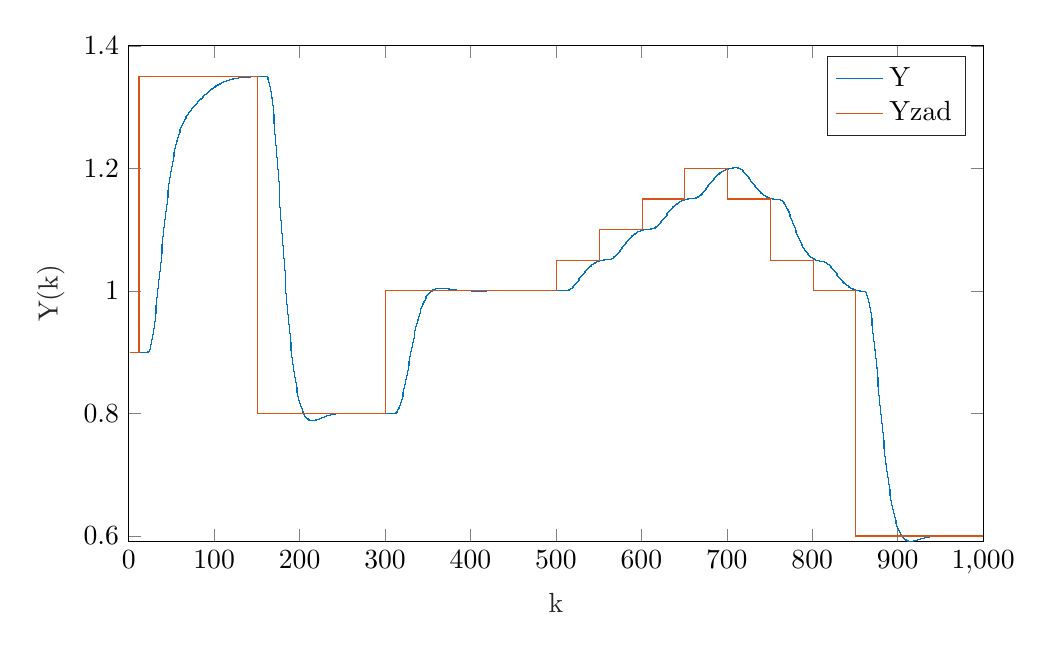
\begin{tikzpicture}

\begin{axis}[%
width=4.272in,
height=2.477in,
at={(0.717in,0.437in)},
scale only axis,
xmin=0,
xmax=1000,
xlabel style={font=\color{white!15!black}},
xlabel={k},
ymin=0.591422105043494,
ymax=1.4,
ylabel style={font=\color{white!15!black}},
ylabel={Y(k)},
axis background/.style={fill=white},
legend style={legend cell align=left, align=left, draw=white!15!black}
]
\addplot[const plot, color=mycolor1] table[row sep=crcr] {%
1	0.9\\
2	0.9\\
3	0.9\\
4	0.9\\
5	0.9\\
6	0.9\\
7	0.9\\
8	0.9\\
9	0.9\\
10	0.9\\
11	0.9\\
12	0.9\\
13	0.9\\
14	0.9\\
15	0.9\\
16	0.9\\
17	0.9\\
18	0.9\\
19	0.9\\
20	0.9\\
21	0.9\\
22	0.900316006479924\\
23	0.901472895106595\\
24	0.903836519989756\\
25	0.907642548238397\\
26	0.913021216391295\\
27	0.92001850802071\\
28	0.928614194576094\\
29	0.938710145141537\\
30	0.950086816415713\\
31	0.962473526352968\\
32	0.975634949036258\\
33	0.989367158241148\\
34	1.00349408131114\\
35	1.01786432264642\\
36	1.03234832003047\\
37	1.04683580057049\\
38	1.06123288951534\\
39	1.07545482637386\\
40	1.08942159926969\\
41	1.10305967349606\\
42	1.11630334610695\\
43	1.1290957078317\\
44	1.14138922235334\\
45	1.15314595236069\\
46	1.16433747388757\\
47	1.17494452701438\\
48	1.18495645386267\\
49	1.19437047820913\\
50	1.20319088243724\\
51	1.21142813045171\\
52	1.21909797443284\\
53	1.22622057438257\\
54	1.2328196520439\\
55	1.23892169472808\\
56	1.24455521965963\\
57	1.24975010547604\\
58	1.25453699434674\\
59	1.25894676567843\\
60	1.2630100804401\\
61	1.26675699367685\\
62	1.27021663170705\\
63	1.2734169297424\\
64	1.2763844251771\\
65	1.27914410151007\\
66	1.28171927775137\\
67	1.2841315381839\\
68	1.28640069747476\\
69	1.28854479633229\\
70	1.2905801231629\\
71	1.29252125748005\\
72	1.29438113114139\\
73	1.29617110382736\\
74	1.29790104951683\\
75	1.29957945105441\\
76	1.30121350023481\\
77	1.30280920114712\\
78	1.30437147482345\\
79	1.30590426351886\\
80	1.30741063321267\\
81	1.30889287316268\\
82	1.31035259156476\\
83	1.3117908065696\\
84	1.31320803208741\\
85	1.31460435797004\\
86	1.31597952430012\\
87	1.3173329896383\\
88	1.31866399318497\\
89	1.31997161090188\\
90	1.32125480571434\\
91	1.32251247197599\\
92	1.32374347442845\\
93	1.32494668192685\\
94	1.32612099623196\\
95	1.32726537619068\\
96	1.3283788576401\\
97	1.32946056937762\\
98	1.33050974554112\\
99	1.33152573474004\\
100	1.33250800627105\\
101	1.33345615374164\\
102	1.33436989641196\\
103	1.33524907855007\\
104	1.33609366707946\\
105	1.33690374777962\\
106	1.33767952028221\\
107	1.33842129208665\\
108	1.33912947179977\\
109	1.3398045617858\\
110	1.3404471503944\\
111	1.34105790391669\\
112	1.34163755840216\\
113	1.34218691145312\\
114	1.34270681409777\\
115	1.3431981628285\\
116	1.34366189187886\\
117	1.34409896579958\\
118	1.34451037238315\\
119	1.34489711597547\\
120	1.34526021120395\\
121	1.34560067714279\\
122	1.34591953192842\\
123	1.3462177878316\\
124	1.34649644678656\\
125	1.34675649637257\\
126	1.34699890623902\\
127	1.3472246249612\\
128	1.34743457731106\\
129	1.34762966192483\\
130	1.34781074934722\\
131	1.3479786804306\\
132	1.34813426506655\\
133	1.34827828122629\\
134	1.34841147428653\\
135	1.34853455661685\\
136	1.3486482074053\\
137	1.34875307269907\\
138	1.348849765638\\
139	1.34893886685911\\
140	1.34902092505164\\
141	1.34909645764278\\
142	1.34916595159546\\
143	1.34922986430079\\
144	1.34928862454872\\
145	1.34934263356177\\
146	1.34939226607788\\
147	1.34943787146964\\
148	1.34947977488804\\
149	1.34951827842046\\
150	1.34955366225323\\
151	1.34958618583049\\
152	1.34961608900189\\
153	1.34964359315255\\
154	1.34966890230989\\
155	1.34969220422227\\
156	1.34971367140576\\
157	1.34973346215546\\
158	1.34975172151886\\
159	1.34976858222929\\
160	1.34978416559774\\
161	1.34941235222008\\
162	1.34801172836376\\
163	1.3451352309734\\
164	1.34049490615522\\
165	1.3339316519948\\
166	1.32538933545457\\
167	1.31489274304814\\
168	1.30252888681627\\
169	1.28843124184815\\
170	1.27276654007964\\
171	1.25572378811602\\
172	1.23750521503019\\
173	1.21831889004938\\
174	1.19837278026136\\
175	1.17787004537723\\
176	1.15700539055931\\
177	1.13596231968896\\
178	1.11491115049826\\
179	1.09400766997486\\
180	1.07339232359273\\
181	1.05318984541932\\
182	1.03350924817459\\
183	1.01444410302314\\
184	0.996073048402831\\
185	0.978460475653423\\
186	0.961657346714703\\
187	0.945702105812197\\
188	0.930621652926231\\
189	0.916432352025124\\
190	0.903141051605342\\
191	0.890746099083877\\
192	0.87923833408818\\
193	0.868602048738367\\
194	0.858815905662033\\
195	0.849853806766285\\
196	0.841685707752935\\
197	0.834278375036275\\
198	0.827596083043515\\
199	0.821601251215823\\
200	0.816255021087248\\
201	0.811517774485115\\
202	0.807349594554667\\
203	0.803710671832258\\
204	0.800561657993067\\
205	0.797863970196893\\
206	0.795580049163569\\
207	0.793673574240611\\
208	0.792109638791625\\
209	0.790854889244815\\
210	0.789877631106067\\
211	0.789147905168518\\
212	0.788637537047564\\
213	0.788320163043241\\
214	0.788171235186377\\
215	0.788168008165775\\
216	0.788289510665098\\
217	0.788516503463698\\
218	0.788831426478638\\
219	0.789218336748005\\
220	0.789662839180728\\
221	0.790152011727083\\
222	0.790674326458526\\
223	0.791219567886513\\
224	0.791778749698471\\
225	0.792344030945809\\
226	0.792908632584165\\
227	0.793466755140391\\
228	0.794013498164127\\
229	0.794544782014302\\
230	0.795057272432374\\
231	0.795548308264436\\
232	0.796015832613189\\
233	0.796458327627891\\
234	0.796874753075398\\
235	0.797264488777871\\
236	0.797627280952221\\
237	0.797963192442441\\
238	0.798272556798207\\
239	0.798555936121163\\
240	0.798814082573417\\
241	0.799047903420723\\
242	0.799258429465111\\
243	0.799446786707906\\
244	0.799614171073829\\
245	0.799761826019729\\
246	0.799891022847151\\
247	0.800003043536014\\
248	0.800099165916873\\
249	0.800180651001256\\
250	0.80024873229312\\
251	0.800304606909339\\
252	0.800349428343028\\
253	0.800384300710294\\
254	0.800410274328449\\
255	0.800428342481627\\
256	0.800439439238062\\
257	0.800444438191741\\
258	0.800444152009779\\
259	0.800439332675412\\
260	0.800430672325032\\
261	0.800418804585998\\
262	0.800404306330094\\
263	0.80038769976529\\
264	0.800369454796025\\
265	0.800349991589354\\
266	0.800329683291114\\
267	0.800308858842641\\
268	0.8002878058546\\
269	0.800266773500051\\
270	0.800245975394079\\
271	0.800225592432109\\
272	0.800205775563393\\
273	0.800186648480222\\
274	0.800168310206982\\
275	0.800150837576542\\
276	0.800134287584346\\
277	0.800118699613252\\
278	0.800104097524465\\
279	0.800090491611978\\
280	0.800077880419685\\
281	0.800066252421897\\
282	0.800055587569285\\
283	0.800045858703379\\
284	0.800037032843675\\
285	0.800029072352125\\
286	0.800021935980398\\
287	0.800015579805727\\
288	0.800009958061494\\
289	0.800005023868911\\
290	0.800000729876281\\
291	0.799997028812361\\
292	0.799993873960294\\
293	0.7999912195585\\
294	0.799989021134751\\
295	0.799987235779475\\
296	0.799985822364079\\
297	0.799984741709866\\
298	0.799983956712804\\
299	0.799983432429143\\
300	0.799983136126559\\
301	0.799983037305202\\
302	0.799983107692715\\
303	0.799983321216995\\
304	0.799983653960142\\
305	0.799984084096789\\
306	0.799984591819667\\
307	0.799985159255041\\
308	0.799985770370355\\
309	0.799986410876196\\
310	0.799987068124442\\
311	0.800128178328655\\
312	0.80064300988468\\
313	0.801694156269134\\
314	0.803386351295231\\
315	0.805777471870803\\
316	0.808887950169963\\
317	0.812708791693216\\
318	0.817208373207934\\
319	0.822338174663277\\
320	0.828037581541662\\
321	0.834237878466594\\
322	0.840865540994476\\
323	0.847844920167989\\
324	0.855100403420225\\
325	0.862558125634539\\
326	0.870147295448086\\
327	0.877801194117295\\
328	0.885457897336448\\
329	0.893060764223975\\
330	0.900558732184566\\
331	0.907906451447103\\
332	0.915064288705834\\
333	0.921998225399391\\
334	0.928679672699636\\
335	0.935085222206015\\
336	0.941196348611654\\
337	0.946999078307795\\
338	0.952483635574797\\
339	0.957644076035888\\
340	0.962477915567401\\
341	0.966985761398123\\
342	0.971170950852876\\
343	0.975039202082695\\
344	0.97859828015863\\
345	0.981857681073\\
346	0.98482833547653\\
347	0.987522333369588\\
348	0.989952670449044\\
349	0.992133016378555\\
350	0.994077504889849\\
351	0.995800545327146\\
352	0.997316655008385\\
353	0.99864031158834\\
354	0.999785824463618\\
355	1.00076722415213\\
356	1.00159816850475\\
357	1.0022918645598\\
358	1.0028610048277\\
359	1.00331771678947\\
360	1.00367352440607\\
361	1.00393932046222\\
362	1.00412534860602\\
363	1.00424119399221\\
364	1.00429578149009\\
365	1.00429738047503\\
366	1.00425361528397\\
367	1.00417148047911\\
368	1.00405736012784\\
369	1.00391705037226\\
370	1.00375578462452\\
371	1.00357826078693\\
372	1.00338866995607\\
373	1.00319072612743\\
374	1.00298769647292\\
375	1.00278243181509\\
376	1.00257739697129\\
377	1.00237470068635\\
378	1.00217612491502\\
379	1.0019831532543\\
380	1.00179699836172\\
381	1.00161862822805\\
382	1.00144879120255\\
383	1.00128803969527\\
384	1.0011367525045\\
385	1.00099515573839\\
386	1.00086334231811\\
387	1.00074129006592\\
388	1.00062887839501\\
389	1.00052590362993\\
390	1.00043209299586\\
391	1.0003471173232\\
392	1.00027060252024\\
393	1.00020213987184\\
394	1.00014129522553\\
395	1.00008761712935\\
396	1.00004064398704\\
397	0.999999910297014\\
398	0.999964952041494\\
399	0.999935311291395\\
400	0.999910540091267\\
401	0.999890203686841\\
402	0.999873883155584\\
403	0.999861177498187\\
404	0.999851705246206\\
405	0.999845105638225\\
406	0.999841039413846\\
407	0.999839189271771\\
408	0.999839260035102\\
409	0.99984097856384\\
410	0.99984409345153\\
411	0.999848374539904\\
412	0.999853612282487\\
413	0.999859616985248\\
414	0.999866217949665\\
415	0.999873262540961\\
416	0.999880615201812\\
417	0.999888156429493\\
418	0.999895781732251\\
419	0.999903400578668\\
420	0.999910935351875\\
421	0.999918320318767\\
422	0.999925500622734\\
423	0.999932431307011\\
424	0.999939076374376\\
425	0.999945407887774\\
426	0.999951405115357\\
427	0.999957053722455\\
428	0.999962345012187\\
429	0.999967275215645\\
430	0.999971844831948\\
431	0.999976058017914\\
432	0.999979922026599\\
433	0.999983446693591\\
434	0.999986643969555\\
435	0.999989527497323\\
436	0.999992112231556\\
437	0.999994414098874\\
438	0.999996449696211\\
439	0.999998236025094\\
440	0.999999790259483\\
441	1.00000112954482\\
442	1.0000022708259\\
443	1.00000323070129\\
444	1.00000402530204\\
445	1.00000467019236\\
446	1.00000518029039\\
447	1.00000556980686\\
448	1.00000585219974\\
449	1.00000604014316\\
450	1.00000614550885\\
451	1.00000617935849\\
452	1.00000615194548\\
453	1.00000607272486\\
454	1.00000595037002\\
455	1.00000579279507\\
456	1.00000560718187\\
457	1.00000540001074\\
458	1.00000517709395\\
459	1.00000494361137\\
460	1.00000470414736\\
461	1.00000446272859\\
462	1.00000422286203\\
463	1.00000398757278\\
464	1.00000375944126\\
465	1.00000354063954\\
466	1.00000333296638\\
467	1.00000313788088\\
468	1.00000295653446\\
469	1.00000278980103\\
470	1.00000263830524\\
471	1.00000250244877\\
472	1.00000238243447\\
473	1.00000227828864\\
474	1.00000218988123\\
475	1.00000211694421\\
476	1.00000205908833\\
477	1.00000201581836\\
478	1.00000198654714\\
479	1.00000197060867\\
480	1.00000196727056\\
481	1.00000197574577\\
482	1.00000199520386\\
483	1.00000202478173\\
484	1.0000020635938\\
485	1.00000211074163\\
486	1.00000216532304\\
487	1.00000222639753\\
488	1.00000229293118\\
489	1.00000236377523\\
490	1.00000243766847\\
491	1.00000251325583\\
492	1.00000258911696\\
493	1.00000266380013\\
494	1.00000273585794\\
495	1.00000280388218\\
496	1.00000286653615\\
497	1.00000292258298\\
498	1.0000029709095\\
499	1.00000301054499\\
500	1.00000304067498\\
501	1.00000306065017\\
502	1.00000306999068\\
503	1.00000306838619\\
504	1.00000305569235\\
505	1.00000303192395\\
506	1.00000299724555\\
507	1.00000295195984\\
508	1.00000289649447\\
509	1.00000283138765\\
510	1.00000275727302\\
511	1.00003778669532\\
512	1.00016623995121\\
513	1.0004287683248\\
514	1.00085155791257\\
515	1.00144908032401\\
516	1.00222644573567\\
517	1.00318140741745\\
518	1.0043060612289\\
519	1.00558827860912\\
520	1.00701290717564\\
521	1.00856276913727\\
522	1.01021948425274\\
523	1.01196414097946\\
524	1.01377783670978\\
525	1.01564210554593\\
526	1.01753924988574\\
527	1.01945259014869\\
528	1.02136664524024\\
529	1.02326725480821\\
530	1.02514165296823\\
531	1.02697850194824\\
532	1.028767893009\\
533	1.03050132102402\\
534	1.03217163823692\\
535	1.03377299194503\\
536	1.03530075017573\\
537	1.03675141881745\\
538	1.03812255313331\\
539	1.03941266611353\\
540	1.04062113570833\\
541	1.04174811261921\\
542	1.04279443000797\\
543	1.04376151620592\\
544	1.0446513112651\\
545	1.04546618798559\\
546	1.04620887787479\\
547	1.04688240234236\\
548	1.0474900093057\\
549	1.04803511527261\\
550	1.04852125287805\\
551	1.0489520237781\\
552	1.04933105674472\\
553	1.04966197075794\\
554	1.04994834285575\\
555	1.05019368047523\\
556	1.05040139799972\\
557	1.05057479721507\\
558	1.05071705137209\\
559	1.05083119255165\\
560	1.05092010203171\\
561	1.05102161519379\\
562	1.05119661287846\\
563	1.05148814228629\\
564	1.05192462035901\\
565	1.05252258568208\\
566	1.05328905415631\\
567	1.05422352734328\\
568	1.05531969678463\\
569	1.05656688263676\\
570	1.05795124057071\\
571	1.0594567669917\\
572	1.06106612917513\\
573	1.06276134384246\\
574	1.06452432496747\\
575	1.06633731917001\\
576	1.06818324488781\\
577	1.07004594958537\\
578	1.07191039753846\\
579	1.07376279919783\\
580	1.07559069176833\\
581	1.07738297942059\\
582	1.07912994046665\\
583	1.08082320786423\\
584	1.0824557285546\\
585	1.08402170637521\\
586	1.08551653261042\\
587	1.08693670764313\\
588	1.08827975663941\\
589	1.08954414172969\\
590	1.0907291727376\\
591	1.09183491814613\\
592	1.0928621176735\\
593	1.09381209755597\\
594	1.09468668939439\\
595	1.09548815321498\\
596	1.09621910521644\\
597	1.09688245052379\\
598	1.09748132114028\\
599	1.09801901918064\\
600	1.0984989653784\\
601	1.0989246527862\\
602	1.09929960552772\\
603	1.09962734241235\\
604	1.09991134518661\\
605	1.10015503116912\\
606	1.10036172999603\\
607	1.10053466419162\\
608	1.10067693327206\\
609	1.10079150108847\\
610	1.10088118611821\\
611	1.10098376624997\\
612	1.1011600699803\\
613	1.10145309712474\\
614	1.10189122198494\\
615	1.10249094501836\\
616	1.10325924826357\\
617	1.10419560343006\\
618	1.10529367595683\\
619	1.10654276338466\\
620	1.10792900199469\\
621	1.10943637177051\\
622	1.11104752628253\\
623	1.11274447101993\\
624	1.11450911096198\\
625	1.11632368574726\\
626	1.11817110863176\\
627	1.1200352234961\\
628	1.12190099244028\\
629	1.12375462497012\\
630	1.12558365841154\\
631	1.12737699796984\\
632	1.12912492376508\\
633	1.13081907120803\\
634	1.13245239022136\\
635	1.13401908804661\\
636	1.13551455969992\\
637	1.13693530953883\\
638	1.13827886687154\\
639	1.13954369807175\\
640	1.14072911724955\\
641	1.14183519716734\\
642	1.14286268177281\\
643	1.14381290144529\\
644	1.14468769181208\\
645	1.14548931678439\\
646	1.14622039628471\\
647	1.14688383898527\\
648	1.14748278024868\\
649	1.1480205253534\\
650	1.1485004979964\\
651	1.14892619399157\\
652	1.14930114002213\\
653	1.14962885725769\\
654	1.14991282960994\\
655	1.15015647637312\\
656	1.15036312897625\\
657	1.15053601156136\\
658	1.15067822509563\\
659	1.15079273472335\\
660	1.15088236006638\\
661	1.15098488001876\\
662	1.15116112395262\\
663	1.15145409243883\\
664	1.15189216042338\\
665	1.15249182890614\\
666	1.15326008037488\\
667	1.15419638690357\\
668	1.15529441421884\\
669	1.15654346007983\\
670	1.15792966092385\\
671	1.15943699683498\\
672	1.16104812143449\\
673	1.16274504021833\\
674	1.16450965813354\\
675	1.16632421475197\\
676	1.16817162323265\\
677	1.17003572733277\\
678	1.17190148900591\\
679	1.1737551175918\\
680	1.17558415023366\\
681	1.17737749194046\\
682	1.17912542262504\\
683	1.18081957748283\\
684	1.18245290621549\\
685	1.18401961584035\\
686	1.18551510114838\\
687	1.18693586626234\\
688	1.1882794402323\\
689	1.18954428914509\\
690	1.19072972679582\\
691	1.1918358256084\\
692	1.1928633291757\\
693	1.19381356751436\\
694	1.19468837589004\\
695	1.19549001786213\\
696	1.19622111301911\\
697	1.19688456972417\\
698	1.19748352306178\\
699	1.19802127806784\\
700	1.19850125823581\\
701	1.19892695921738\\
702	1.19930190757585\\
703	1.19962962440335\\
704	1.19991359357554\\
705	1.20015723439039\\
706	1.20036387831809\\
707	1.20053674957639\\
708	1.2006789492394\\
709	1.20079344258595\\
710	1.20088304939634\\
711	1.20091532508079\\
712	1.2008344601689\\
713	1.20060215452511\\
714	1.20019441284226\\
715	1.19959879488789\\
716	1.19881206480083\\
717	1.19783819011011\\
718	1.19668664678449\\
719	1.1953709916108\\
720	1.19390766762282\\
721	1.19231501222802\\
722	1.19061244116719\\
723	1.1888197845434\\
724	1.18695675391757\\
725	1.18504252192619\\
726	1.18309539806847\\
727	1.18113258626332\\
728	1.17917001151898\\
729	1.17722220461163\\
730	1.17530223505508\\
731	1.17342168387813\\
732	1.17159064882735\\
733	1.16981777559214\\
734	1.1681103095207\\
735	1.16647416306985\\
736	1.16491399491837\\
737	1.16343329727125\\
738	1.16203448843644\\
739	1.16071900823783\\
740	1.15948741422918\\
741	1.15833947704035\\
742	1.15727427350723\\
743	1.15629027651566\\
744	1.15538544073152\\
745	1.1545572835975\\
746	1.15380296115634\\
747	1.15311933841232\\
748	1.15250305407237\\
749	1.1519505796157\\
750	1.15145827273087\\
751	1.15102242523235\\
752	1.15063930562792\\
753	1.15030519655437\\
754	1.15001642733498\\
755	1.14976940193814\\
756	1.14956062263455\\
757	1.14938670966141\\
758	1.14924441720715\\
759	1.14913064603046\\
760	1.14904245302307\\
761	1.14890683435654\\
762	1.14860453811684\\
763	1.14805181996829\\
764	1.14719403572369\\
765	1.14600013849937\\
766	1.14445796973465\\
767	1.14257024605715\\
768	1.14035115519985\\
769	1.13782348410835\\
770	1.1350162111762\\
771	1.13196250235127\\
772	1.12869805778687\\
773	1.12525976187127\\
774	1.12168459494951\\
775	1.11800876992997\\
776	1.11426706131422\\
777	1.11049229806179\\
778	1.10671499515409\\
779	1.10296310180016\\
780	1.09926184697105\\
781	1.09563366539554\\
782	1.09209818932879\\
783	1.08867229334514\\
784	1.08537018113174\\
785	1.08220350479264\\
786	1.07918150853281\\
787	1.07631118978586\\
788	1.07359747193084\\
789	1.07104338369113\\
790	1.06865024111933\\
791	1.06641782879862\\
792	1.06434457752593\\
793	1.06242773629602\\
794	1.06066353688609\\
795	1.05904734975516\\
796	1.05757383032933\\
797	1.05623705504789\\
798	1.05503064680349\\
799	1.05394788962578\\
800	1.05298183263855\\
801	1.05212538346795\\
802	1.05137139139917\\
803	1.05071272067381\\
804	1.05014231439319\\
805	1.04965324954744\\
806	1.04923878372827\\
807	1.04889239410759\\
808	1.04860780927708\\
809	1.0483790345457\\
810	1.04820037128715\\
811	1.04803131908501\\
812	1.04780848904271\\
813	1.04748648542774\\
814	1.04703470296818\\
815	1.04643457400036\\
816	1.04567721044411\\
817	1.0447613919106\\
818	1.04369185683644\\
819	1.0424778584808\\
820	1.04113195199865\\
821	1.03966898268324\\
822	1.03810524891439\\
823	1.03645781640794\\
824	1.03474396308162\\
825	1.03298073627306\\
826	1.03118460620038\\
827	1.02937120147595\\
828	1.02755511419445\\
829	1.02574976364122\\
830	1.02396730902577\\
831	1.02221860285641\\
832	1.0205131776502\\
833	1.01885925963282\\
834	1.0172638039366\\
835	1.01573254656407\\
836	1.01427006905702\\
837	1.01287987239746\\
838	1.01156445721043\\
839	1.01032540781196\\
840	1.00916347803986\\
841	1.00807867716469\\
842	1.00707035449415\\
843	1.00613728155905\\
844	1.00527773100797\\
845	1.0044895515442\\
846	1.00377023841644\\
847	1.0031169991265\\
848	1.00252681414627\\
849	1.0019964925448\\
850	1.00152272251695\\
851	1.00110211687954\\
852	1.00073125366178\\
853	1.00040671196469\\
854	1.00012510330217\\
855	0.999883098664412\\
856	0.999677451564431\\
857	0.999505017342186\\
858	0.999362769007659\\
859	0.999247809907037\\
860	0.999157383494241\\
861	0.998807985836111\\
862	0.99773060356738\\
863	0.995597730601543\\
864	0.99219773828798\\
865	0.987412868961282\\
866	0.981200409281216\\
867	0.973576650620023\\
868	0.964603288704274\\
869	0.954375954498904\\
870	0.943014603569788\\
871	0.930655522430905\\
872	0.917444738152061\\
873	0.903532642189088\\
874	0.889069661361982\\
875	0.874202828462069\\
876	0.859073122391365\\
877	0.843813463265436\\
878	0.828547261754896\\
879	0.81338743428421\\
880	0.798435806711361\\
881	0.783782838920673\\
882	0.769507611499451\\
883	0.755678023448635\\
884	0.74235115679724\\
885	0.729573770138045\\
886	0.717382888556428\\
887	0.705806462266322\\
888	0.694864070522239\\
889	0.684567651136355\\
890	0.674922239261253\\
891	0.665926702007416\\
892	0.6575744580082\\
893	0.649854173261287\\
894	0.642750426498603\\
895	0.636244338997079\\
896	0.630314165168566\\
897	0.624935841483923\\
898	0.620083492316877\\
899	0.615729892158632\\
900	0.611846884373255\\
901	0.60840575725392\\
902	0.605377578616551\\
903	0.602733490544551\\
904	0.600444966188687\\
905	0.598484030741476\\
906	0.596823448855796\\
907	0.595436880872303\\
908	0.594299010267876\\
909	0.593385644745164\\
910	0.592673793358073\\
911	0.592141722015509\\
912	0.591768989631155\\
913	0.591536467095167\\
914	0.591426341138262\\
915	0.591422105043494\\
916	0.591508538038945\\
917	0.591671675078308\\
918	0.591898768588105\\
919	0.59217824363204\\
920	0.592499647816219\\
921	0.592853597135076\\
922	0.593231718837872\\
923	0.593626592280401\\
924	0.594031688616759\\
925	0.594441310082147\\
926	0.594850529520077\\
927	0.595255130716216\\
928	0.595651550016522\\
929	0.596036819629416\\
930	0.596408512940324\\
931	0.596764692101931\\
932	0.597103858104709\\
933	0.597424903479413\\
934	0.597727067736123\\
935	0.598009895602647\\
936	0.59827319808847\\
937	0.59851701638997\\
938	0.598741588592331\\
939	0.598947319084554\\
940	0.599134750616553\\
941	0.599304538910266\\
942	0.599457429722944\\
943	0.599594238250037\\
944	0.599715830747034\\
945	0.599823108243925\\
946	0.599916992222353\\
947	0.599998412123806\\
948	0.600068294557057\\
949	0.600127554074289\\
950	0.600177085387736\\
951	0.600217756902078\\
952	0.600250405441993\\
953	0.600275832059088\\
954	0.600294798807802\\
955	0.600308026385556\\
956	0.60031619253842\\
957	0.600319931139726\\
958	0.600319831855257\\
959	0.60031644031491\\
960	0.600310258716875\\
961	0.600301746796449\\
962	0.600291323097495\\
963	0.600279366490247\\
964	0.600266217884649\\
965	0.600252182093613\\
966	0.600237529805531\\
967	0.600222499630049\\
968	0.600207300185466\\
969	0.600192112200196\\
970	0.600177090604532\\
971	0.600162366592403\\
972	0.600148049636042\\
973	0.600134229439383\\
974	0.600120977818654\\
975	0.600108350501014\\
976	0.600096388834242\\
977	0.600085121402356\\
978	0.600074565543764\\
979	0.600064728770005\\
980	0.600055610084472\\
981	0.600047201201641\\
982	0.600039487668289\\
983	0.600032449889021\\
984	0.600026064059069\\
985	0.600020303007889\\
986	0.600015136957504\\
987	0.600010534210595\\
988	0.600006461767113\\
989	0.600002885860476\\
990	0.599999772420544\\
991	0.599997087470075\\
992	0.599994797460909\\
993	0.599992869555722\\
994	0.599991271860766\\
995	0.599989973614655\\
996	0.599988945337885\\
997	0.599988158947447\\
998	0.599987587840554\\
999	0.599987206951208\\
1000	0.599986992783039\\
};
\addlegendentry{Y}

\addplot[const plot, color=mycolor2] table[row sep=crcr] {%
1	0.9\\
2	0.9\\
3	0.9\\
4	0.9\\
5	0.9\\
6	0.9\\
7	0.9\\
8	0.9\\
9	0.9\\
10	0.9\\
11	0.9\\
12	1.35\\
13	1.35\\
14	1.35\\
15	1.35\\
16	1.35\\
17	1.35\\
18	1.35\\
19	1.35\\
20	1.35\\
21	1.35\\
22	1.35\\
23	1.35\\
24	1.35\\
25	1.35\\
26	1.35\\
27	1.35\\
28	1.35\\
29	1.35\\
30	1.35\\
31	1.35\\
32	1.35\\
33	1.35\\
34	1.35\\
35	1.35\\
36	1.35\\
37	1.35\\
38	1.35\\
39	1.35\\
40	1.35\\
41	1.35\\
42	1.35\\
43	1.35\\
44	1.35\\
45	1.35\\
46	1.35\\
47	1.35\\
48	1.35\\
49	1.35\\
50	1.35\\
51	1.35\\
52	1.35\\
53	1.35\\
54	1.35\\
55	1.35\\
56	1.35\\
57	1.35\\
58	1.35\\
59	1.35\\
60	1.35\\
61	1.35\\
62	1.35\\
63	1.35\\
64	1.35\\
65	1.35\\
66	1.35\\
67	1.35\\
68	1.35\\
69	1.35\\
70	1.35\\
71	1.35\\
72	1.35\\
73	1.35\\
74	1.35\\
75	1.35\\
76	1.35\\
77	1.35\\
78	1.35\\
79	1.35\\
80	1.35\\
81	1.35\\
82	1.35\\
83	1.35\\
84	1.35\\
85	1.35\\
86	1.35\\
87	1.35\\
88	1.35\\
89	1.35\\
90	1.35\\
91	1.35\\
92	1.35\\
93	1.35\\
94	1.35\\
95	1.35\\
96	1.35\\
97	1.35\\
98	1.35\\
99	1.35\\
100	1.35\\
101	1.35\\
102	1.35\\
103	1.35\\
104	1.35\\
105	1.35\\
106	1.35\\
107	1.35\\
108	1.35\\
109	1.35\\
110	1.35\\
111	1.35\\
112	1.35\\
113	1.35\\
114	1.35\\
115	1.35\\
116	1.35\\
117	1.35\\
118	1.35\\
119	1.35\\
120	1.35\\
121	1.35\\
122	1.35\\
123	1.35\\
124	1.35\\
125	1.35\\
126	1.35\\
127	1.35\\
128	1.35\\
129	1.35\\
130	1.35\\
131	1.35\\
132	1.35\\
133	1.35\\
134	1.35\\
135	1.35\\
136	1.35\\
137	1.35\\
138	1.35\\
139	1.35\\
140	1.35\\
141	1.35\\
142	1.35\\
143	1.35\\
144	1.35\\
145	1.35\\
146	1.35\\
147	1.35\\
148	1.35\\
149	1.35\\
150	1.35\\
151	0.8\\
152	0.8\\
153	0.8\\
154	0.8\\
155	0.8\\
156	0.8\\
157	0.8\\
158	0.8\\
159	0.8\\
160	0.8\\
161	0.8\\
162	0.8\\
163	0.8\\
164	0.8\\
165	0.8\\
166	0.8\\
167	0.8\\
168	0.8\\
169	0.8\\
170	0.8\\
171	0.8\\
172	0.8\\
173	0.8\\
174	0.8\\
175	0.8\\
176	0.8\\
177	0.8\\
178	0.8\\
179	0.8\\
180	0.8\\
181	0.8\\
182	0.8\\
183	0.8\\
184	0.8\\
185	0.8\\
186	0.8\\
187	0.8\\
188	0.8\\
189	0.8\\
190	0.8\\
191	0.8\\
192	0.8\\
193	0.8\\
194	0.8\\
195	0.8\\
196	0.8\\
197	0.8\\
198	0.8\\
199	0.8\\
200	0.8\\
201	0.8\\
202	0.8\\
203	0.8\\
204	0.8\\
205	0.8\\
206	0.8\\
207	0.8\\
208	0.8\\
209	0.8\\
210	0.8\\
211	0.8\\
212	0.8\\
213	0.8\\
214	0.8\\
215	0.8\\
216	0.8\\
217	0.8\\
218	0.8\\
219	0.8\\
220	0.8\\
221	0.8\\
222	0.8\\
223	0.8\\
224	0.8\\
225	0.8\\
226	0.8\\
227	0.8\\
228	0.8\\
229	0.8\\
230	0.8\\
231	0.8\\
232	0.8\\
233	0.8\\
234	0.8\\
235	0.8\\
236	0.8\\
237	0.8\\
238	0.8\\
239	0.8\\
240	0.8\\
241	0.8\\
242	0.8\\
243	0.8\\
244	0.8\\
245	0.8\\
246	0.8\\
247	0.8\\
248	0.8\\
249	0.8\\
250	0.8\\
251	0.8\\
252	0.8\\
253	0.8\\
254	0.8\\
255	0.8\\
256	0.8\\
257	0.8\\
258	0.8\\
259	0.8\\
260	0.8\\
261	0.8\\
262	0.8\\
263	0.8\\
264	0.8\\
265	0.8\\
266	0.8\\
267	0.8\\
268	0.8\\
269	0.8\\
270	0.8\\
271	0.8\\
272	0.8\\
273	0.8\\
274	0.8\\
275	0.8\\
276	0.8\\
277	0.8\\
278	0.8\\
279	0.8\\
280	0.8\\
281	0.8\\
282	0.8\\
283	0.8\\
284	0.8\\
285	0.8\\
286	0.8\\
287	0.8\\
288	0.8\\
289	0.8\\
290	0.8\\
291	0.8\\
292	0.8\\
293	0.8\\
294	0.8\\
295	0.8\\
296	0.8\\
297	0.8\\
298	0.8\\
299	0.8\\
300	0.8\\
301	1\\
302	1\\
303	1\\
304	1\\
305	1\\
306	1\\
307	1\\
308	1\\
309	1\\
310	1\\
311	1\\
312	1\\
313	1\\
314	1\\
315	1\\
316	1\\
317	1\\
318	1\\
319	1\\
320	1\\
321	1\\
322	1\\
323	1\\
324	1\\
325	1\\
326	1\\
327	1\\
328	1\\
329	1\\
330	1\\
331	1\\
332	1\\
333	1\\
334	1\\
335	1\\
336	1\\
337	1\\
338	1\\
339	1\\
340	1\\
341	1\\
342	1\\
343	1\\
344	1\\
345	1\\
346	1\\
347	1\\
348	1\\
349	1\\
350	1\\
351	1\\
352	1\\
353	1\\
354	1\\
355	1\\
356	1\\
357	1\\
358	1\\
359	1\\
360	1\\
361	1\\
362	1\\
363	1\\
364	1\\
365	1\\
366	1\\
367	1\\
368	1\\
369	1\\
370	1\\
371	1\\
372	1\\
373	1\\
374	1\\
375	1\\
376	1\\
377	1\\
378	1\\
379	1\\
380	1\\
381	1\\
382	1\\
383	1\\
384	1\\
385	1\\
386	1\\
387	1\\
388	1\\
389	1\\
390	1\\
391	1\\
392	1\\
393	1\\
394	1\\
395	1\\
396	1\\
397	1\\
398	1\\
399	1\\
400	1\\
401	1\\
402	1\\
403	1\\
404	1\\
405	1\\
406	1\\
407	1\\
408	1\\
409	1\\
410	1\\
411	1\\
412	1\\
413	1\\
414	1\\
415	1\\
416	1\\
417	1\\
418	1\\
419	1\\
420	1\\
421	1\\
422	1\\
423	1\\
424	1\\
425	1\\
426	1\\
427	1\\
428	1\\
429	1\\
430	1\\
431	1\\
432	1\\
433	1\\
434	1\\
435	1\\
436	1\\
437	1\\
438	1\\
439	1\\
440	1\\
441	1\\
442	1\\
443	1\\
444	1\\
445	1\\
446	1\\
447	1\\
448	1\\
449	1\\
450	1\\
451	1\\
452	1\\
453	1\\
454	1\\
455	1\\
456	1\\
457	1\\
458	1\\
459	1\\
460	1\\
461	1\\
462	1\\
463	1\\
464	1\\
465	1\\
466	1\\
467	1\\
468	1\\
469	1\\
470	1\\
471	1\\
472	1\\
473	1\\
474	1\\
475	1\\
476	1\\
477	1\\
478	1\\
479	1\\
480	1\\
481	1\\
482	1\\
483	1\\
484	1\\
485	1\\
486	1\\
487	1\\
488	1\\
489	1\\
490	1\\
491	1\\
492	1\\
493	1\\
494	1\\
495	1\\
496	1\\
497	1\\
498	1\\
499	1\\
500	1\\
501	1.05\\
502	1.05\\
503	1.05\\
504	1.05\\
505	1.05\\
506	1.05\\
507	1.05\\
508	1.05\\
509	1.05\\
510	1.05\\
511	1.05\\
512	1.05\\
513	1.05\\
514	1.05\\
515	1.05\\
516	1.05\\
517	1.05\\
518	1.05\\
519	1.05\\
520	1.05\\
521	1.05\\
522	1.05\\
523	1.05\\
524	1.05\\
525	1.05\\
526	1.05\\
527	1.05\\
528	1.05\\
529	1.05\\
530	1.05\\
531	1.05\\
532	1.05\\
533	1.05\\
534	1.05\\
535	1.05\\
536	1.05\\
537	1.05\\
538	1.05\\
539	1.05\\
540	1.05\\
541	1.05\\
542	1.05\\
543	1.05\\
544	1.05\\
545	1.05\\
546	1.05\\
547	1.05\\
548	1.05\\
549	1.05\\
550	1.05\\
551	1.1\\
552	1.1\\
553	1.1\\
554	1.1\\
555	1.1\\
556	1.1\\
557	1.1\\
558	1.1\\
559	1.1\\
560	1.1\\
561	1.1\\
562	1.1\\
563	1.1\\
564	1.1\\
565	1.1\\
566	1.1\\
567	1.1\\
568	1.1\\
569	1.1\\
570	1.1\\
571	1.1\\
572	1.1\\
573	1.1\\
574	1.1\\
575	1.1\\
576	1.1\\
577	1.1\\
578	1.1\\
579	1.1\\
580	1.1\\
581	1.1\\
582	1.1\\
583	1.1\\
584	1.1\\
585	1.1\\
586	1.1\\
587	1.1\\
588	1.1\\
589	1.1\\
590	1.1\\
591	1.1\\
592	1.1\\
593	1.1\\
594	1.1\\
595	1.1\\
596	1.1\\
597	1.1\\
598	1.1\\
599	1.1\\
600	1.1\\
601	1.15\\
602	1.15\\
603	1.15\\
604	1.15\\
605	1.15\\
606	1.15\\
607	1.15\\
608	1.15\\
609	1.15\\
610	1.15\\
611	1.15\\
612	1.15\\
613	1.15\\
614	1.15\\
615	1.15\\
616	1.15\\
617	1.15\\
618	1.15\\
619	1.15\\
620	1.15\\
621	1.15\\
622	1.15\\
623	1.15\\
624	1.15\\
625	1.15\\
626	1.15\\
627	1.15\\
628	1.15\\
629	1.15\\
630	1.15\\
631	1.15\\
632	1.15\\
633	1.15\\
634	1.15\\
635	1.15\\
636	1.15\\
637	1.15\\
638	1.15\\
639	1.15\\
640	1.15\\
641	1.15\\
642	1.15\\
643	1.15\\
644	1.15\\
645	1.15\\
646	1.15\\
647	1.15\\
648	1.15\\
649	1.15\\
650	1.15\\
651	1.2\\
652	1.2\\
653	1.2\\
654	1.2\\
655	1.2\\
656	1.2\\
657	1.2\\
658	1.2\\
659	1.2\\
660	1.2\\
661	1.2\\
662	1.2\\
663	1.2\\
664	1.2\\
665	1.2\\
666	1.2\\
667	1.2\\
668	1.2\\
669	1.2\\
670	1.2\\
671	1.2\\
672	1.2\\
673	1.2\\
674	1.2\\
675	1.2\\
676	1.2\\
677	1.2\\
678	1.2\\
679	1.2\\
680	1.2\\
681	1.2\\
682	1.2\\
683	1.2\\
684	1.2\\
685	1.2\\
686	1.2\\
687	1.2\\
688	1.2\\
689	1.2\\
690	1.2\\
691	1.2\\
692	1.2\\
693	1.2\\
694	1.2\\
695	1.2\\
696	1.2\\
697	1.2\\
698	1.2\\
699	1.2\\
700	1.2\\
701	1.15\\
702	1.15\\
703	1.15\\
704	1.15\\
705	1.15\\
706	1.15\\
707	1.15\\
708	1.15\\
709	1.15\\
710	1.15\\
711	1.15\\
712	1.15\\
713	1.15\\
714	1.15\\
715	1.15\\
716	1.15\\
717	1.15\\
718	1.15\\
719	1.15\\
720	1.15\\
721	1.15\\
722	1.15\\
723	1.15\\
724	1.15\\
725	1.15\\
726	1.15\\
727	1.15\\
728	1.15\\
729	1.15\\
730	1.15\\
731	1.15\\
732	1.15\\
733	1.15\\
734	1.15\\
735	1.15\\
736	1.15\\
737	1.15\\
738	1.15\\
739	1.15\\
740	1.15\\
741	1.15\\
742	1.15\\
743	1.15\\
744	1.15\\
745	1.15\\
746	1.15\\
747	1.15\\
748	1.15\\
749	1.15\\
750	1.15\\
751	1.05\\
752	1.05\\
753	1.05\\
754	1.05\\
755	1.05\\
756	1.05\\
757	1.05\\
758	1.05\\
759	1.05\\
760	1.05\\
761	1.05\\
762	1.05\\
763	1.05\\
764	1.05\\
765	1.05\\
766	1.05\\
767	1.05\\
768	1.05\\
769	1.05\\
770	1.05\\
771	1.05\\
772	1.05\\
773	1.05\\
774	1.05\\
775	1.05\\
776	1.05\\
777	1.05\\
778	1.05\\
779	1.05\\
780	1.05\\
781	1.05\\
782	1.05\\
783	1.05\\
784	1.05\\
785	1.05\\
786	1.05\\
787	1.05\\
788	1.05\\
789	1.05\\
790	1.05\\
791	1.05\\
792	1.05\\
793	1.05\\
794	1.05\\
795	1.05\\
796	1.05\\
797	1.05\\
798	1.05\\
799	1.05\\
800	1.05\\
801	1\\
802	1\\
803	1\\
804	1\\
805	1\\
806	1\\
807	1\\
808	1\\
809	1\\
810	1\\
811	1\\
812	1\\
813	1\\
814	1\\
815	1\\
816	1\\
817	1\\
818	1\\
819	1\\
820	1\\
821	1\\
822	1\\
823	1\\
824	1\\
825	1\\
826	1\\
827	1\\
828	1\\
829	1\\
830	1\\
831	1\\
832	1\\
833	1\\
834	1\\
835	1\\
836	1\\
837	1\\
838	1\\
839	1\\
840	1\\
841	1\\
842	1\\
843	1\\
844	1\\
845	1\\
846	1\\
847	1\\
848	1\\
849	1\\
850	1\\
851	0.6\\
852	0.6\\
853	0.6\\
854	0.6\\
855	0.6\\
856	0.6\\
857	0.6\\
858	0.6\\
859	0.6\\
860	0.6\\
861	0.6\\
862	0.6\\
863	0.6\\
864	0.6\\
865	0.6\\
866	0.6\\
867	0.6\\
868	0.6\\
869	0.6\\
870	0.6\\
871	0.6\\
872	0.6\\
873	0.6\\
874	0.6\\
875	0.6\\
876	0.6\\
877	0.6\\
878	0.6\\
879	0.6\\
880	0.6\\
881	0.6\\
882	0.6\\
883	0.6\\
884	0.6\\
885	0.6\\
886	0.6\\
887	0.6\\
888	0.6\\
889	0.6\\
890	0.6\\
891	0.6\\
892	0.6\\
893	0.6\\
894	0.6\\
895	0.6\\
896	0.6\\
897	0.6\\
898	0.6\\
899	0.6\\
900	0.6\\
901	0.6\\
902	0.6\\
903	0.6\\
904	0.6\\
905	0.6\\
906	0.6\\
907	0.6\\
908	0.6\\
909	0.6\\
910	0.6\\
911	0.6\\
912	0.6\\
913	0.6\\
914	0.6\\
915	0.6\\
916	0.6\\
917	0.6\\
918	0.6\\
919	0.6\\
920	0.6\\
921	0.6\\
922	0.6\\
923	0.6\\
924	0.6\\
925	0.6\\
926	0.6\\
927	0.6\\
928	0.6\\
929	0.6\\
930	0.6\\
931	0.6\\
932	0.6\\
933	0.6\\
934	0.6\\
935	0.6\\
936	0.6\\
937	0.6\\
938	0.6\\
939	0.6\\
940	0.6\\
941	0.6\\
942	0.6\\
943	0.6\\
944	0.6\\
945	0.6\\
946	0.6\\
947	0.6\\
948	0.6\\
949	0.6\\
950	0.6\\
951	0.6\\
952	0.6\\
953	0.6\\
954	0.6\\
955	0.6\\
956	0.6\\
957	0.6\\
958	0.6\\
959	0.6\\
960	0.6\\
961	0.6\\
962	0.6\\
963	0.6\\
964	0.6\\
965	0.6\\
966	0.6\\
967	0.6\\
968	0.6\\
969	0.6\\
970	0.6\\
971	0.6\\
972	0.6\\
973	0.6\\
974	0.6\\
975	0.6\\
976	0.6\\
977	0.6\\
978	0.6\\
979	0.6\\
980	0.6\\
981	0.6\\
982	0.6\\
983	0.6\\
984	0.6\\
985	0.6\\
986	0.6\\
987	0.6\\
988	0.6\\
989	0.6\\
990	0.6\\
991	0.6\\
992	0.6\\
993	0.6\\
994	0.6\\
995	0.6\\
996	0.6\\
997	0.6\\
998	0.6\\
999	0.6\\
1000	0.6\\
};
\addlegendentry{Yzad}

\end{axis}
\end{tikzpicture}%
\caption{Wyjście DMC dla parametrów $N=100$, $N_u=10$, $\lambda=50$}
\end{figure}

\begin{equation}
E = 18,4148
\end{equation}

Zwiększając jeszcze bardziej $\lambda$ widzimy że regulacja przy dużym skoku jest szybsza, natomiast przy częstych małych zmianach wartości zadanej regulacjia działą gorzej.

\begin{figure}[H]
\centering
% This file was created by matlab2tikz.
%
%The latest updates can be retrieved from
%  http://www.mathworks.com/matlabcentral/fileexchange/22022-matlab2tikz-matlab2tikz
%where you can also make suggestions and rate matlab2tikz.
%
\definecolor{mycolor1}{rgb}{0.00000,0.44700,0.74100}%
%
\begin{tikzpicture}

\begin{axis}[%
width=4.272in,
height=2.477in,
at={(0.717in,0.437in)},
scale only axis,
xmin=0,
xmax=1000,
xlabel style={font=\color{white!15!black}},
xlabel={k},
ymin=2.5,
ymax=3.4,
ylabel style={font=\color{white!15!black}},
ylabel={U(k)},
axis background/.style={fill=white}
]
\addplot[const plot, color=mycolor1, forget plot] table[row sep=crcr] {%
1	3\\
2	3\\
3	3\\
4	3\\
5	3\\
6	3\\
7	3\\
8	3\\
9	3\\
10	3\\
11	3\\
12	3.03677723762225\\
13	3.06987794549847\\
14	3.09961282286456\\
15	3.12626892357163\\
16	3.15011145140538\\
17	3.17138539386811\\
18	3.19031701331497\\
19	3.20711521177891\\
20	3.22197278361128\\
21	3.23506756816011\\
22	3.24656351306771\\
23	3.25661165735666\\
24	3.26535104225986\\
25	3.27290955670733\\
26	3.27940472348883\\
27	3.28494443134491\\
28	3.28962761758287\\
29	3.29354490525325\\
30	3.29677919844252\\
31	3.29940623882755\\
32	3.3\\
33	3.3\\
34	3.3\\
35	3.3\\
36	3.3\\
37	3.3\\
38	3.29999674099907\\
39	3.29979028782618\\
40	3.29941175588972\\
41	3.29888902912539\\
42	3.29824767275958\\
43	3.29751167552349\\
44	3.29670323562673\\
45	3.29584242203398\\
46	3.29494698856832\\
47	3.29403230668209\\
48	3.29311138997263\\
49	3.29219507310449\\
50	3.29129228369774\\
51	3.29041028470094\\
52	3.28955489024796\\
53	3.28873065769594\\
54	3.28794105827166\\
55	3.28718862851064\\
56	3.2864751044564\\
57	3.28580154039186\\
58	3.28516841369942\\
59	3.28457571728867\\
60	3.28402304088875\\
61	3.28350964237449\\
62	3.28303451018031\\
63	3.28259641775206\\
64	3.28219397089314\\
65	3.28182564877692\\
66	3.28148983932067\\
67	3.28118486954751\\
68	3.28090903150032\\
69	3.28066060421515\\
70	3.28043787221057\\
71	3.28023914090322\\
72	3.28006274931812\\
73	3.27990708042434\\
74	3.27977056939257\\
75	3.27965171003989\\
76	3.27954905969944\\
77	3.27946124272695\\
78	3.27938695283343\\
79	3.27932495441252\\
80	3.27927408301233\\
81	3.27923324508471\\
82	3.27920141712954\\
83	3.27917764433825\\
84	3.27916103882778\\
85	3.27915077754584\\
86	3.27914609991759\\
87	3.27914630529537\\
88	3.27915075032867\\
89	3.27915884615564\\
90	3.27917005553972\\
91	3.27918388998512\\
92	3.27919990685973\\
93	3.27921770654915\\
94	3.2792369296621\\
95	3.27925725430352\\
96	3.27927839342867\\
97	3.27930009228878\\
98	3.27932212597641\\
99	3.27934429707665\\
100	3.27936643342823\\
101	3.27938838599735\\
102	3.27941002686534\\
103	3.27943124733047\\
104	3.27945195612293\\
105	3.2794720777313\\
106	3.27949155083825\\
107	3.27951032686239\\
108	3.27952836860303\\
109	3.27954564898405\\
110	3.27956214989289\\
111	3.2795778611104\\
112	3.27959277932737\\
113	3.27960690724313\\
114	3.27962025274194\\
115	3.27963282814262\\
116	3.27964464951718\\
117	3.27965573607396\\
118	3.27966610960121\\
119	3.27967579396698\\
120	3.27968481467136\\
121	3.27969319844728\\
122	3.27970097290613\\
123	3.27970816622488\\
124	3.27971480687119\\
125	3.27972092336353\\
126	3.27972654406313\\
127	3.27973169699518\\
128	3.27973640969642\\
129	3.27974070908678\\
130	3.27974462136272\\
131	3.27974817191005\\
132	3.27975138523431\\
133	3.27975428490676\\
134	3.27975689352432\\
135	3.27975923268184\\
136	3.27976132295517\\
137	3.27976318389383\\
138	3.27976483402188\\
139	3.27976629084601\\
140	3.27976757086968\\
141	3.27976868961255\\
142	3.27976966163413\\
143	3.2797705005612\\
144	3.27977121911793\\
145	3.27977182915849\\
146	3.27977234170127\\
147	3.27977276696443\\
148	3.27977311440228\\
149	3.27977339274209\\
150	3.27977361002103\\
151	3.23482381652914\\
152	3.1943675124835\\
153	3.15802496055937\\
154	3.12544532280052\\
155	3.09630446637397\\
156	3.07030296675822\\
157	3.04716428527513\\
158	3.0266331010009\\
159	3.00847377979006\\
160	2.99246896547411\\
161	2.97841828030193\\
162	2.96613712341496\\
163	2.95545555763397\\
164	2.94621727610815\\
165	2.93827864147009\\
166	2.93150779107691\\
167	2.92578380271927\\
168	2.92099591586626\\
169	2.91704280410015\\
170	2.91383189489627\\
171	2.91127873333159\\
172	2.90930638667117\\
173	2.90784488709459\\
174	2.90683071009158\\
175	2.90620628628514\\
176	2.90591954463715\\
177	2.90592348516045\\
178	2.90617577940767\\
179	2.90663839713351\\
180	2.90727725763521\\
181	2.90806190437258\\
182	2.90896520155669\\
183	2.90996305147255\\
184	2.9110341313688\\
185	2.91215964880893\\
186	2.91332311443465\\
187	2.91451013114337\\
188	2.91570819181127\\
189	2.91690650728687\\
190	2.91809583896627\\
191	2.91926834428276\\
192	2.92041743431956\\
193	2.92153764279182\\
194	2.9226245056791\\
195	2.92367445082354\\
196	2.92468469684219\\
197	2.92565316073342\\
198	2.92657837358832\\
199	2.92745940384766\\
200	2.92829578757412\\
201	2.92908746523712\\
202	2.92983472453492\\
203	2.93053814880473\\
204	2.93119857059697\\
205	2.93181703001394\\
206	2.93239473743718\\
207	2.93293304028994\\
208	2.93343339350332\\
209	2.93389733337533\\
210	2.9343264545322\\
211	2.93472238972044\\
212	2.93508679217629\\
213	2.93542132033685\\
214	2.93572762467358\\
215	2.93600733644464\\
216	2.93626205817765\\
217	2.93649335570824\\
218	2.93670275161358\\
219	2.93689171989209\\
220	2.93706168175314\\
221	2.93721400239146\\
222	2.93734998863152\\
223	2.93747088733689\\
224	2.9375778844888\\
225	2.93767210484663\\
226	2.93775461211122\\
227	2.93782640944092\\
228	2.937888440433\\
229	2.93794159040911\\
230	2.93798668795286\\
231	2.93802450665291\\
232	2.93805576701005\\
233	2.93808113847131\\
234	2.93810124155841\\
235	2.93811665006166\\
236	2.93812789327409\\
237	2.93813545824373\\
238	2.93813979202488\\
239	2.938141303912\\
240	2.93814036764214\\
241	2.93813732355415\\
242	2.93813248069462\\
243	2.93812611886272\\
244	2.93811849058712\\
245	2.93810982303003\\
246	2.93810031981442\\
247	2.93809016277171\\
248	2.938079513608\\
249	2.93806851548796\\
250	2.93805729453616\\
251	2.93804596125625\\
252	2.9380346118688\\
253	2.93802332956955\\
254	2.93801218570947\\
255	2.93800124089907\\
256	2.93799054603921\\
257	2.93798014328103\\
258	2.93797006691773\\
259	2.93796034421113\\
260	2.93795099615591\\
261	2.93794203818456\\
262	2.93793348081606\\
263	2.93792533025124\\
264	2.93791758891795\\
265	2.9379102559688\\
266	2.9379033277345\\
267	2.93789679813555\\
268	2.93789065905496\\
269	2.93788490067479\\
270	2.93787951177877\\
271	2.93787448002382\\
272	2.93786979218234\\
273	2.93786543435797\\
274	2.93786139217647\\
275	2.93785765095406\\
276	2.93785419584495\\
277	2.93785101196986\\
278	2.9378480845272\\
279	2.93784539888855\\
280	2.93784294067977\\
281	2.93784069584927\\
282	2.9378386507246\\
283	2.93783679205859\\
284	2.93783510706619\\
285	2.93783358345288\\
286	2.9378322094358\\
287	2.9378309737583\\
288	2.93782986569873\\
289	2.93782887507428\\
290	2.9378279922405\\
291	2.93782720808697\\
292	2.93782651402998\\
293	2.93782590200238\\
294	2.93782536444129\\
295	2.93782489427396\\
296	2.93782448490225\\
297	2.93782413018596\\
298	2.9378238244253\\
299	2.93782356234297\\
300	2.93782333906576\\
301	2.95416858904939\\
302	2.96887985601006\\
303	2.98209522472626\\
304	2.99394227124823\\
305	3.00453886080054\\
306	3.01399387389102\\
307	3.0224078690222\\
308	3.02987368926533\\
309	3.03647701897563\\
310	3.0422968960805\\
311	3.04740618464341\\
312	3.05187201177803\\
313	3.05575617244815\\
314	3.05911550522534\\
315	3.06200224167907\\
316	3.06446433173349\\
317	3.06654574703331\\
318	3.06828676411208\\
319	3.06972422894567\\
320	3.07089180429205\\
321	3.0718202010593\\
322	3.07253739481096\\
323	3.07306882840431\\
324	3.07343760165984\\
325	3.07366464887683\\
326	3.07376890493881\\
327	3.07376746914672\\
328	3.07367573974909\\
329	3.07350755009432\\
330	3.07327529575673\\
331	3.0729900531504\\
332	3.07266169011287\\
333	3.07229896891297\\
334	3.07190964211131\\
335	3.0715005416795\\
336	3.07107766176311\\
337	3.07064623545454\\
338	3.07021080592391\\
339	3.06977529223986\\
340	3.06934305019631\\
341	3.06891692844686\\
342	3.06849932023411\\
343	3.06809221098802\\
344	3.06769722205454\\
345	3.06731565080331\\
346	3.06694850735122\\
347	3.06659654812723\\
348	3.06626030649239\\
349	3.06594012061855\\
350	3.06563615881822\\
351	3.06534844250854\\
352	3.0650768669817\\
353	3.06482122014546\\
354	3.06458119938748\\
355	3.06435642670883\\
356	3.06414646226323\\
357	3.06395081643033\\
358	3.06376896054371\\
359	3.06360033638619\\
360	3.06344436455835\\
361	3.06330045181869\\
362	3.06316799748752\\
363	3.06304639900036\\
364	3.06293505669027\\
365	3.06283337787324\\
366	3.06274078030508\\
367	3.06265669507307\\
368	3.06258056898099\\
369	3.06251186648139\\
370	3.06245007120459\\
371	3.06239468713017\\
372	3.06234523944237\\
373	3.0623012751078\\
374	3.06226236321006\\
375	3.06222809507309\\
376	3.06219808420189\\
377	3.06217196609521\\
378	3.06214939788911\\
379	3.06213005789017\\
380	3.06211364501704\\
381	3.06209987816744\\
382	3.06208849552546\\
383	3.06207925382283\\
384	3.06207192756582\\
385	3.06206630823841\\
386	3.06206220349081\\
387	3.06205943632136\\
388	3.06205784425884\\
389	3.06205727855101\\
390	3.06205760336459\\
391	3.06205869500099\\
392	3.06206044113125\\
393	3.06206274005331\\
394	3.06206549997383\\
395	3.06206863831652\\
396	3.06207208105837\\
397	3.06207576209478\\
398	3.06207962263421\\
399	3.0620836106228\\
400	3.06208768019896\\
401	3.06209179117777\\
402	3.06209590856495\\
403	3.06210000209972\\
404	3.06210404582609\\
405	3.06210801769163\\
406	3.06211189917298\\
407	3.06211567492705\\
408	3.062119332467\\
409	3.06212286186196\\
410	3.06212625545931\\
411	3.06212950762854\\
412	3.06213261452554\\
413	3.06213557387628\\
414	3.06213838477869\\
415	3.06214104752179\\
416	3.06214356342097\\
417	3.06214593466833\\
418	3.06214816419726\\
419	3.06215025556013\\
420	3.06215221281829\\
421	3.06215404044339\\
422	3.0621557432293\\
423	3.06215732621372\\
424	3.06215879460872\\
425	3.06216015373962\\
426	3.06216140899128\\
427	3.06216256576144\\
428	3.06216362942023\\
429	3.06216460527547\\
430	3.06216549854317\\
431	3.06216631432271\\
432	3.06216705757618\\
433	3.06216773311168\\
434	3.06216834556983\\
435	3.06216889941345\\
436	3.06216939891986\\
437	3.06216984817556\\
438	3.06217025107301\\
439	3.0621706113092\\
440	3.06217093238583\\
441	3.06217121761084\\
442	3.06217147010104\\
443	3.06217169278582\\
444	3.06217188841155\\
445	3.0621720595467\\
446	3.06217220858751\\
447	3.062172337764\\
448	3.0621724491463\\
449	3.06217254465119\\
450	3.06217262604875\\
451	3.06217269496904\\
452	3.06217275290872\\
453	3.06217280123763\\
454	3.06217284120519\\
455	3.06217287394659\\
456	3.06217290048881\\
457	3.06217292175627\\
458	3.06217293857625\\
459	3.06217295168396\\
460	3.06217296172731\\
461	3.06217296927156\\
462	3.06217297480406\\
463	3.06217297873911\\
464	3.06217298142312\\
465	3.06217298314025\\
466	3.06217298411861\\
467	3.06217298453713\\
468	3.06217298453328\\
469	3.06217298421076\\
470	3.06217298364592\\
471	3.06217298289329\\
472	3.06217298199015\\
473	3.06217298096046\\
474	3.06217297981804\\
475	3.06217297856924\\
476	3.06217297721512\\
477	3.06217297267834\\
478	3.06217296271297\\
479	3.0621729457636\\
480	3.06217292084358\\
481	3.06217288742985\\
482	3.06217284537264\\
483	3.06217279481803\\
484	3.062172736142\\
485	3.06217266989439\\
486	3.06217259675167\\
487	3.06217251747735\\
488	3.06217243288898\\
489	3.06217234383105\\
490	3.0621722511528\\
491	3.06217215569043\\
492	3.06217205825302\\
493	3.06217195961164\\
494	3.06217186049122\\
495	3.06217176156467\\
496	3.06217166344901\\
497	3.06217156670309\\
498	3.06217147182669\\
499	3.06217137926074\\
500	3.06217128938837\\
501	3.06625756227257\\
502	3.06993533514601\\
503	3.0732391303688\\
504	3.07620084298841\\
505	3.07884994022283\\
506	3.08121364299544\\
507	3.0833170916202\\
508	3.08518349745246\\
509	3.08683428207461\\
510	3.08828920537483\\
511	3.08956648369449\\
512	3.09068289906304\\
513	3.09165390040424\\
514	3.09249369748194\\
515	3.09321534825403\\
516	3.0938308402183\\
517	3.09435116626084\\
518	3.0947863954555\\
519	3.09514573920928\\
520	3.09543761310346\\
521	3.09566969474081\\
522	3.09584897787644\\
523	3.09598182308124\\
524	3.09607400516241\\
525	3.09613075754513\\
526	3.09615681380114\\
527	3.09615644649489\\
528	3.09613350350461\\
529	3.09609144196395\\
530	3.09603335996006\\
531	3.09596202611503\\
532	3.09587990716986\\
533	3.0957891936833\\
534	3.09569182395163\\
535	3.09558950624996\\
536	3.0954837394904\\
537	3.09537583238794\\
538	3.09526692122038\\
539	3.09515798626469\\
540	3.09504986698826\\
541	3.09494327607007\\
542	3.09483881232307\\
543	3.09473697258607\\
544	3.09463816265002\\
545	3.09454270728069\\
546	3.09445085939657\\
547	3.09436280845827\\
548	3.09427868812267\\
549	3.09419858321246\\
550	3.09412253604907\\
551	3.09813691193051\\
552	3.10174682181283\\
553	3.10498673495189\\
554	3.10788847067813\\
555	3.11048140166196\\
556	3.11279263883205\\
557	3.11484720007767\\
558	3.11666816458009\\
559	3.11827681437094\\
560	3.11969276450182\\
561	3.12093408302557\\
562	3.12201740183104\\
563	3.12295801923663\\
564	3.12376999513063\\
565	3.12446623934568\\
566	3.12505859386789\\
567	3.12555790940749\\
568	3.12597411679372\\
569	3.12631629360272\\
570	3.12659272638026\\
571	3.12681096878132\\
572	3.12697789591437\\
573	3.12709975514873\\
574	3.12718221361847\\
575	3.12723040263454\\
576	3.12724895919835\\
577	3.12724206480078\\
578	3.127213481654\\
579	3.12716658651626\\
580	3.12710440225025\\
581	3.12702962724616\\
582	3.12694466283248\\
583	3.12685163879005\\
584	3.12675243707861\\
585	3.12664871387885\\
586	3.12654192004779\\
587	3.1264333200801\\
588	3.12632400966372\\
589	3.12621493191334\\
590	3.1261068923618\\
591	3.12600057278519\\
592	3.12589654393408\\
593	3.12579527723981\\
594	3.12569715556132\\
595	3.12560248303496\\
596	3.12551149408658\\
597	3.12542436166233\\
598	3.12534120473148\\
599	3.12526209511225\\
600	3.1251870636685\\
601	3.12920246565873\\
602	3.13281340329609\\
603	3.13605433827601\\
604	3.13895708344381\\
605	3.14155100595989\\
606	3.14386321212447\\
607	3.14591871599276\\
608	3.14774059362549\\
609	3.1493501245722\\
610	3.15076692197147\\
611	3.15200905246827\\
612	3.15309314698981\\
613	3.15403450328504\\
614	3.15484718101555\\
615	3.15554409008477\\
616	3.15613707280605\\
617	3.15663698043583\\
618	3.15705374453478\\
619	3.1573964435651\\
620	3.15767336508579\\
621	3.15789206386759\\
622	3.15805941621523\\
623	3.15818167075524\\
624	3.1582644959225\\
625	3.1583130243571\\
626	3.15833189440448\\
627	3.15832528890284\\
628	3.15829697140478\\
629	3.15825031999349\\
630	3.15818835883368\\
631	3.15811378758849\\
632	3.1580290088251\\
633	3.15793615352462\\
634	3.15783710480527\\
635	3.15773351996185\\
636	3.15762685091916\\
637	3.15751836319209\\
638	3.1574091534403\\
639	3.15730016570148\\
640	3.15719220638266\\
641	3.1570859580858\\
642	3.15698199233961\\
643	3.1568807813068\\
644	3.15678270853199\\
645	3.15668807879279\\
646	3.15659712711334\\
647	3.15651002699656\\
648	3.1564268979286\\
649	3.15634781220627\\
650	3.1562728011354\\
651	3.16028822038149\\
652	3.16389917253142\\
653	3.16714011962264\\
654	3.17004287481249\\
655	3.17263680554482\\
656	3.17494901837631\\
657	3.17700452759302\\
658	3.17882640946228\\
659	3.18043594371723\\
660	3.18185274365827\\
661	3.18309487607154\\
662	3.18417897200596\\
663	3.18512032931396\\
664	3.18593300774366\\
665	3.18662991726946\\
666	3.18722290026168\\
667	3.18772280802146\\
668	3.1881395721438\\
669	3.18848227111683\\
670	3.18875919251861\\
671	3.18897789113352\\
672	3.18914524327562\\
673	3.18926749757744\\
674	3.18935032247733\\
675	3.189398850617\\
676	3.18941772034215\\
677	3.1894111137217\\
678	3.18938279374679\\
679	3.18933613811178\\
680	3.18927417073476\\
681	3.18919959114813\\
682	3.18911480188166\\
683	3.18902193395302\\
684	3.18892287057446\\
685	3.18881926917826\\
686	3.18871258185839\\
687	3.18860407432064\\
688	3.18849484342909\\
689	3.18838583343257\\
690	3.18827785095048\\
691	3.18817157879383\\
692	3.18806758869365\\
693	3.18796635300544\\
694	3.18786825545506\\
695	3.18777360098839\\
696	3.18768262478384\\
697	3.18759550048408\\
698	3.18751234770021\\
699	3.1874332388393\\
700	3.18735820530299\\
701	3.18320088336697\\
702	3.17945610176838\\
703	3.17608927832575\\
704	3.17306843649549\\
705	3.17036400957958\\
706	3.16794866248995\\
707	3.16579712900239\\
708	3.16388606271484\\
709	3.16219390016821\\
710	3.16070073479793\\
711	3.15938820056493\\
712	3.15823936426985\\
713	3.15723862568785\\
714	3.15637162477549\\
715	3.15562515529923\\
716	3.1549870843187\\
717	3.15444627702974\\
718	3.15399252653319\\
719	3.1536164881473\\
720	3.15330961792626\\
721	3.1530641150853\\
722	3.15287286806539\\
723	3.15272940399785\\
724	3.15262784135281\\
725	3.15256284557547\\
726	3.15252958753123\\
727	3.15252370383398\\
728	3.1525412614042\\
729	3.1525787233676\\
730	3.15263291718012\\
731	3.15270100485625\\
732	3.15278045518444\\
733	3.15286901782025\\
734	3.15296469915341\\
735	3.15306573985077\\
736	3.15317059398136\\
737	3.1532779096345\\
738	3.1533865109462\\
739	3.1534953814524\\
740	3.15360364869188\\
741	3.15371056998451\\
742	3.1538155193143\\
743	3.15391797524959\\
744	3.15401750983574\\
745	3.15411377839894\\
746	3.15420651020223\\
747	3.15429549989783\\
748	3.15438059972256\\
749	3.15446171238559\\
750	3.1545387846006\\
751	3.14643908174494\\
752	3.13915234757094\\
753	3.1326095834968\\
754	3.12674706916981\\
755	3.12150595962268\\
756	3.11683191873228\\
757	3.11267478475021\\
758	3.10898826424503\\
759	3.10572965128839\\
760	3.10285956914228\\
761	3.10034173207131\\
762	3.09814272521885\\
763	3.0962318007578\\
764	3.0945806887595\\
765	3.09316342142448\\
766	3.09195616949063\\
767	3.09093708978111\\
768	3.09008618298037\\
769	3.08938516083434\\
770	3.08881732206271\\
771	3.0883674363505\\
772	3.08802163585364\\
773	3.08776731371092\\
774	3.08759302910417\\
775	3.08748841845084\\
776	3.08744411234993\\
777	3.08745165715747\\
778	3.08750344340169\\
779	3.08759263797312\\
780	3.08771312083071\\
781	3.08785942596506\\
782	3.08802668637619\\
783	3.08821058283712\\
784	3.08840729622777\\
785	3.08861346323498\\
786	3.08882613522513\\
787	3.08904274010554\\
788	3.08926104699978\\
789	3.08947913357042\\
790	3.08969535583063\\
791	3.08990832029366\\
792	3.090116858316\\
793	3.09032000249717\\
794	3.09051696500536\\
795	3.09070711770445\\
796	3.09088997396413\\
797	3.09106517204033\\
798	3.09123245991933\\
799	3.09139168152374\\
800	3.09154276418449\\
801	3.08759934755171\\
802	3.08405635584259\\
803	3.08087938062912\\
804	3.0780366849545\\
805	3.0754989963847\\
806	3.07323931879887\\
807	3.07123276075565\\
808	3.0694563785605\\
809	3.06788903240829\\
810	3.06651125419062\\
811	3.0653051257432\\
812	3.06425416646879\\
813	3.06334322940928\\
814	3.0625584049593\\
815	3.06188693151586\\
816	3.06131711244663\\
817	3.06083823883452\\
818	3.06044051752135\\
819	3.0601150040286\\
820	3.05985353998071\\
821	3.05964869469805\\
822	3.05949371066134\\
823	3.05938245257988\\
824	3.0593093598217\\
825	3.05926940198614\\
826	3.05925803741873\\
827	3.05927117370209\\
828	3.05930513250056\\
829	3.05935661582535\\
830	3.05942267459264\\
831	3.0595006793385\\
832	3.05958829296383\\
833	3.05968344538972\\
834	3.05978431001108\\
835	3.05988928184239\\
836	3.0599969572553\\
837	3.06010611521331\\
838	3.06021569991325\\
839	3.06032480474825\\
840	3.06043265751089\\
841	3.06053860675947\\
842	3.06064210927386\\
843	3.06074271853147\\
844	3.06084007413691\\
845	3.06093389214242\\
846	3.06102395619952\\
847	3.06111010948496\\
848	3.06119224734753\\
849	3.06127031062462\\
850	3.06134427958059\\
851	3.02872329053498\\
852	2.99936629101073\\
853	2.97299717163522\\
854	2.94936086168166\\
855	2.92822172964407\\
856	2.90936212778626\\
857	2.89258106384079\\
858	2.87769298530846\\
859	2.86452666377387\\
860	2.85292416834664\\
861	2.84273991879868\\
862	2.83383981022442\\
863	2.82610040213162\\
864	2.81940816579861\\
865	2.81365878452976\\
866	2.80875650212357\\
867	2.8046135154522\\
868	2.80114940755114\\
869	2.79829061804564\\
870	2.79596994810602\\
871	2.79412609743599\\
872	2.79270323106494\\
873	2.79165057394349\\
874	2.79092203153669\\
875	2.7904758347769\\
876	2.79027420788174\\
877	2.79028305842795\\
878	2.79047168591907\\
879	2.7908125104244\\
880	2.79128081918169\\
881	2.79185453014446\\
882	2.79251397151746\\
883	2.79324167637913\\
884	2.79402219153999\\
885	2.79484189983065\\
886	2.79568885505423\\
887	2.79655262887569\\
888	2.79742416895559\\
889	2.79829566766828\\
890	2.79916044077567\\
891	2.8000128154563\\
892	2.80084802711765\\
893	2.80166212444595\\
894	2.80245188217318\\
895	2.80321472106587\\
896	2.80394863466345\\
897	2.80465212231759\\
898	2.80532412810549\\
899	2.80596398521217\\
900	2.80657136539741\\
901	2.80714623318325\\
902	2.80768880441753\\
903	2.80819950888813\\
904	2.80867895668039\\
905	2.80912790798839\\
906	2.80954724610751\\
907	2.80993795335204\\
908	2.81030108965774\\
909	2.81063777364385\\
910	2.81094916592405\\
911	2.81123645446921\\
912	2.81150084183846\\
913	2.81174353410735\\
914	2.81196573133418\\
915	2.81216861941693\\
916	2.81235336320384\\
917	2.81252110073142\\
918	2.8126729384728\\
919	2.81280994748944\\
920	2.81293316038782\\
921	2.81304356898996\\
922	2.81314212263464\\
923	2.81322972703306\\
924	2.81330724360946\\
925	2.81337548926337\\
926	2.81343523649616\\
927	2.81348721533038\\
928	2.8135321120748\\
929	2.8135705703348\\
930	2.8136031921956\\
931	2.81363053954582\\
932	2.81365313551214\\
933	2.81367146597925\\
934	2.81368598117209\\
935	2.81369709728033\\
936	2.81370519810726\\
937	2.81371063672764\\
938	2.81371373714136\\
939	2.81371479591117\\
940	2.81371408377487\\
941	2.81371184722374\\
942	2.81370831004025\\
943	2.81370367478953\\
944	2.81369812426015\\
945	2.81369182285052\\
946	2.81368491789856\\
947	2.81367754095255\\
948	2.81366980898219\\
949	2.81366182552911\\
950	2.81365368179695\\
951	2.8136454576814\\
952	2.81363722274081\\
953	2.81362903710867\\
954	2.81362095234928\\
955	2.81361301225817\\
956	2.81360525360906\\
957	2.81359770684936\\
958	2.81359039674616\\
959	2.81358334298485\\
960	2.8135765607226\\
961	2.81357006109868\\
962	2.81356385170399\\
963	2.8135579370118\\
964	2.81355231877197\\
965	2.81354699637064\\
966	2.81354196715758\\
967	2.8135372267431\\
968	2.81353276926654\\
969	2.81352858763844\\
970	2.81352467375857\\
971	2.81352101871143\\
972	2.81351761294103\\
973	2.81351444640631\\
974	2.81351150871901\\
975	2.81350878926511\\
976	2.81350627731139\\
977	2.81350396286699\\
978	2.81350183578677\\
979	2.8134998858758\\
980	2.8134981029788\\
981	2.81349647705604\\
982	2.81349499824707\\
983	2.81349365692371\\
984	2.81349244373329\\
985	2.81349134963349\\
986	2.81349036591951\\
987	2.8134894842447\\
988	2.81348869663526\\
989	2.81348799549995\\
990	2.8134873736354\\
991	2.81348682422752\\
992	2.81348634084981\\
993	2.81348591745887\\
994	2.81348554838758\\
995	2.81348522833642\\
996	2.81348495236329\\
997	2.81348471587206\\
998	2.8134845146002\\
999	2.81348434460577\\
1000	2.81348420225389\\
};
\end{axis}
\end{tikzpicture}%
\caption{Sterowanie DMC dla parametrów $N=100$, $N_u=10$, $\lambda=200$}
\end{figure}

\begin{figure}[H]
\centering
% This file was created by matlab2tikz.
%
%The latest updates can be retrieved from
%  http://www.mathworks.com/matlabcentral/fileexchange/22022-matlab2tikz-matlab2tikz
%where you can also make suggestions and rate matlab2tikz.
%
\definecolor{mycolor1}{rgb}{0.00000,0.44700,0.74100}%
\definecolor{mycolor2}{rgb}{0.85000,0.32500,0.09800}%
%
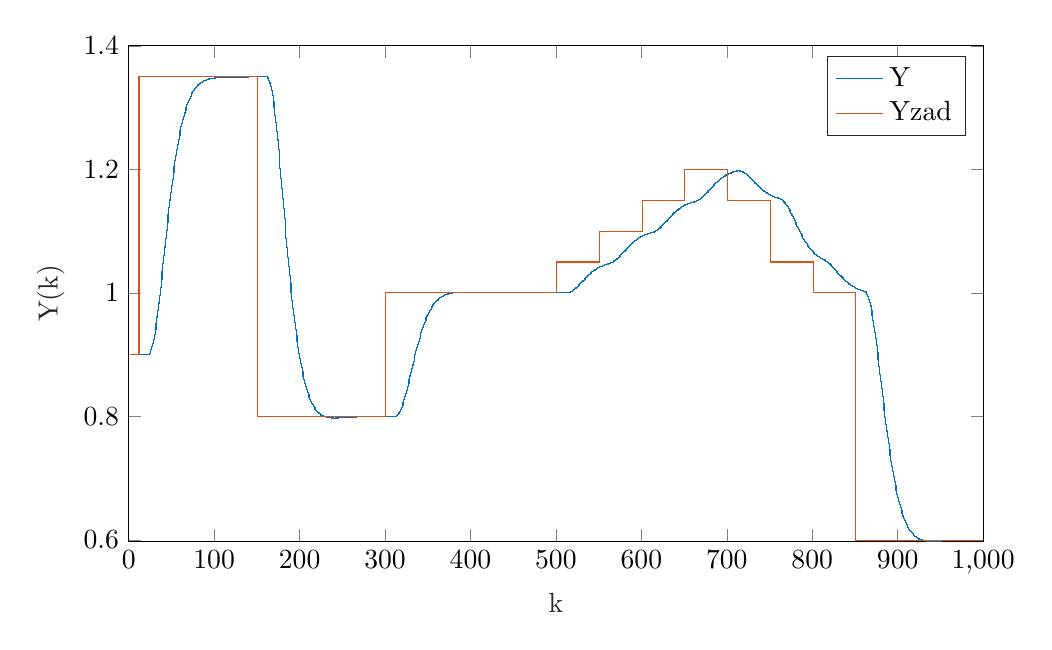
\begin{tikzpicture}

\begin{axis}[%
width=4.272in,
height=2.477in,
at={(0.717in,0.437in)},
scale only axis,
xmin=0,
xmax=1000,
xlabel style={font=\color{white!15!black}},
xlabel={k},
ymin=0.598165940466007,
ymax=1.4,
ylabel style={font=\color{white!15!black}},
ylabel={Y(k)},
axis background/.style={fill=white},
legend style={legend cell align=left, align=left, draw=white!15!black}
]
\addplot[const plot, color=mycolor1] table[row sep=crcr] {%
1	0.9\\
2	0.9\\
3	0.9\\
4	0.9\\
5	0.9\\
6	0.9\\
7	0.9\\
8	0.9\\
9	0.9\\
10	0.9\\
11	0.9\\
12	0.9\\
13	0.9\\
14	0.9\\
15	0.9\\
16	0.9\\
17	0.9\\
18	0.9\\
19	0.9\\
20	0.9\\
21	0.9\\
22	0.900194592041983\\
23	0.90091160929711\\
24	0.902388687830795\\
25	0.904788754505774\\
26	0.908213366229576\\
27	0.912714164769349\\
28	0.918302681031955\\
29	0.924958695751444\\
30	0.932637339566901\\
31	0.941275094180498\\
32	0.95079483736455\\
33	0.961110057776353\\
34	0.972128350608552\\
35	0.98375429184441\\
36	0.995891777118094\\
37	1.00844590073669\\
38	1.02132444115779\\
39	1.0344390110049\\
40	1.04770592242704\\
41	1.06104681216683\\
42	1.07438115413806\\
43	1.08762759088826\\
44	1.10071492657886\\
45	1.11358398337516\\
46	1.12618612340283\\
47	1.13848193160645\\
48	1.15044002583663\\
49	1.16203494242937\\
50	1.17324554908663\\
51	1.18405481414026\\
52	1.19444955678446\\
53	1.20442019130943\\
54	1.21396047048091\\
55	1.22306722697704\\
56	1.23174011215899\\
57	1.2399813329736\\
58	1.2477953887536\\
59	1.25518881068519\\
60	1.26216990753198\\
61	1.26874852091892\\
62	1.27493579261991\\
63	1.28074394558014\\
64	1.28618607981632\\
65	1.29127598385723\\
66	1.2960279619985\\
67	1.30045667733313\\
68	1.30457701027424\\
69	1.30840393209536\\
70	1.3119523928701\\
71	1.31523722308771\\
72	1.31827304814848\\
73	1.32107421489651\\
74	1.32365472932333\\
75	1.32602820456894\\
76	1.32820781835466\\
77	1.33020627900037\\
78	1.33203579920661\\
79	1.33370807681542\\
80	1.33523428180272\\
81	1.33662504879662\\
82	1.33789047446034\\
83	1.3390401191231\\
84	1.34008301208757\\
85	1.34102766008744\\
86	1.34188205841222\\
87	1.34265370425886\\
88	1.34334961191069\\
89	1.34397632938279\\
90	1.34453995620995\\
91	1.34504616208776\\
92	1.34550020611006\\
93	1.34590695637596\\
94	1.34627090976767\\
95	1.34659621172638\\
96	1.34688667587691\\
97	1.34714580337363\\
98	1.34737680186023\\
99	1.34758260395369\\
100	1.34776588517835\\
101	1.34792908129084\\
102	1.34807440494925\\
103	1.34820386169188\\
104	1.34831926520088\\
105	1.3484222518352\\
106	1.34851429442496\\
107	1.3485967153266\\
108	1.34867069874334\\
109	1.34873730232118\\
110	1.34879746803444\\
111	1.34885203237846\\
112	1.34890173589007\\
113	1.34894723201861\\
114	1.34898909537205\\
115	1.34902782936436\\
116	1.34906387329088\\
117	1.3490976088593\\
118	1.34912936620418\\
119	1.34915942941269\\
120	1.34918804158955\\
121	1.34921540948818\\
122	1.34924170773514\\
123	1.3492670826739\\
124	1.3492916558531\\
125	1.34931552718416\\
126	1.34933877779142\\
127	1.3493614725776\\
128	1.34938366252605\\
129	1.34940538676031\\
130	1.3494266743804\\
131	1.34944754609422\\
132	1.34946801566146\\
133	1.34948809116629\\
134	1.34950777613405\\
135	1.34952707050638\\
136	1.34954597148801\\
137	1.34956447427768\\
138	1.34958257269472\\
139	1.34960025971193\\
140	1.34961752790461\\
141	1.34963436982494\\
142	1.3496507783098\\
143	1.34966674673005\\
144	1.34968226918786\\
145	1.34969734066887\\
146	1.34971195715462\\
147	1.34972611570085\\
148	1.34973981448614\\
149	1.34975305283547\\
150	1.34976583122228\\
151	1.34977815125268\\
152	1.34979001563491\\
153	1.34980142813663\\
154	1.34981239353264\\
155	1.34982291754511\\
156	1.34983300677819\\
157	1.34984266864866\\
158	1.34985191131408\\
159	1.3498607435996\\
160	1.34986917492452\\
161	1.34963938051151\\
162	1.3487706857642\\
163	1.34697265737374\\
164	1.34404617359255\\
165	1.33986712064562\\
166	1.33437239234045\\
167	1.32754790700054\\
168	1.31941838879364\\
169	1.31003868980861\\
170	1.29948645526025\\
171	1.28785595732692\\
172	1.27525294367109\\
173	1.26179036494247\\
174	1.24758486176736\\
175	1.23275390611319\\
176	1.21741350468084\\
177	1.20167638329872\\
178	1.18565058132923\\
179	1.16943839399055\\
180	1.15313560837072\\
181	1.13683098587805\\
182	1.12060595003201\\
183	1.10453444393987\\
184	1.08868292660703\\
185	1.07311048146192\\
186	1.05786901420455\\
187	1.04300352036559\\
188	1.02855240584179\\
189	1.01454784619713\\
190	1.00101617272833\\
191	0.98797827522262\\
192	0.975450013018031\\
193	0.96344262743881\\
194	0.951963149947583\\
195	0.941014801452964\\
196	0.93059737915717\\
197	0.920707628140503\\
198	0.911339595537641\\
199	0.902484965806455\\
200	0.894133376118389\\
201	0.886272711267922\\
202	0.878889377851581\\
203	0.871968557758978\\
204	0.865494441257439\\
205	0.859450440144907\\
206	0.853819381599155\\
207	0.848583683470485\\
208	0.843725511854758\\
209	0.839226921848226\\
210	0.835069982428838\\
211	0.831236886433908\\
212	0.827710046614079\\
213	0.824472178741017\\
214	0.821506372733386\\
215	0.818796152744358\\
216	0.816325527125891\\
217	0.814079029151695\\
218	0.812041749343485\\
219	0.810199360204843\\
220	0.80853813412473\\
221	0.807044955169161\\
222	0.805707325435478\\
223	0.804513366599513\\
224	0.803451817242287\\
225	0.802512026500031\\
226	0.801683944539577\\
227	0.800958110320822\\
228	0.800325637069153\\
229	0.799778195843619\\
230	0.799307997551319\\
231	0.798907773725052\\
232	0.798570756349715\\
233	0.79829065699334\\
234	0.79806164547091\\
235	0.797878328243309\\
236	0.797735726729726\\
237	0.79762925568923\\
238	0.797554701806969\\
239	0.79750820260214\\
240	0.797486225757566\\
241	0.797485548954947\\
242	0.797503240285534\\
243	0.797536639292988\\
244	0.797583338693525\\
245	0.797641166807947\\
246	0.79770817073081\\
247	0.797782600253656\\
248	0.797862892551867\\
249	0.797947657638261\\
250	0.798035664580885\\
251	0.798125828477601\\
252	0.798217198175827\\
253	0.798308944722278\\
254	0.798400350524519\\
255	0.798490799203696\\
256	0.798579766115791\\
257	0.798666809517163\\
258	0.798751562348944\\
259	0.798833724613963\\
260	0.798913056319317\\
261	0.798989370957377\\
262	0.799062529497945\\
263	0.799132434864396\\
264	0.799199026866909\\
265	0.799262277566347\\
266	0.799322187042912\\
267	0.799378779544331\\
268	0.799432099989128\\
269	0.799482210801333\\
270	0.799529189053841\\
271	0.799573123898598\\
272	0.799614114262679\\
273	0.79965226679034\\
274	0.799687694012056\\
275	0.799720512722571\\
276	0.799750842550926\\
277	0.79977880470641\\
278	0.799804520885308\\
279	0.799828112324245\\
280	0.79984969898682\\
281	0.799869398871097\\
282	0.799887327426349\\
283	0.799903597068264\\
284	0.799918316782592\\
285	0.799931591807947\\
286	0.799943523389203\\
287	0.799954208593549\\
288	0.799963740181954\\
289	0.799972206529352\\
290	0.799979691587439\\
291	0.799986274884509\\
292	0.799992031557243\\
293	0.79999703240984\\
294	0.800001343996313\\
295	0.80000502872218\\
296	0.800008144962157\\
297	0.8000107471908\\
298	0.800012886123404\\
299	0.8000146088647\\
300	0.800015959063246\\
301	0.8000169770696\\
302	0.800017700096611\\
303	0.80001816238041\\
304	0.800018395340821\\
305	0.800018427740133\\
306	0.800018285839312\\
307	0.800017993550886\\
308	0.800017572587859\\
309	0.800017042608136\\
310	0.800016421354032\\
311	0.800102210138555\\
312	0.800420126901849\\
313	0.801075800452181\\
314	0.802141654095845\\
315	0.80366283430324\\
316	0.805662301843554\\
317	0.808145189342726\\
318	0.811102517239045\\
319	0.814514349462288\\
320	0.818352460698672\\
321	0.822582578694599\\
322	0.827166257581037\\
323	0.83206243156437\\
324	0.837228692436957\\
325	0.842622329129824\\
326	0.848201162888416\\
327	0.853924207535476\\
328	0.859752180635489\\
329	0.865647888141463\\
330	0.87157650224161\\
331	0.877505749589996\\
332	0.883406024865305\\
333	0.889250442623129\\
334	0.895014838660995\\
335	0.900677730575878\\
336	0.906220245838408\\
337	0.911626024560704\\
338	0.916881103021437\\
339	0.921973783060067\\
340	0.926894491713154\\
341	0.931635634762329\\
342	0.936191447250406\\
343	0.940557843489061\\
344	0.944732268619154\\
345	0.948713553384977\\
346	0.952501773439102\\
347	0.956098114198601\\
348	0.959504742020336\\
349	0.962724682247652\\
350	0.965761704498491\\
351	0.968620215411633\\
352	0.971305158939755\\
353	0.973821924172123\\
354	0.976176260583016\\
355	0.978374200532043\\
356	0.980421988786886\\
357	0.982326018795895\\
358	0.98409277540549\\
359	0.985728783693956\\
360	0.987240563577613\\
361	0.988634589836306\\
362	0.989917257201523\\
363	0.99109485015152\\
364	0.992173517062483\\
365	0.993159248372637\\
366	0.994057858426378\\
367	0.994874970677696\\
368	0.995616005945746\\
369	0.996286173430075\\
370	0.996890464208445\\
371	0.997433646955998\\
372	0.997920265640582\\
373	0.998354638965078\\
374	0.998740861343495\\
375	0.999082805213147\\
376	0.99938412450042\\
377	0.999648259072331\\
378	0.999878440020144\\
379	1.00007769563486\\
380	1.00024885794716\\
381	1.00039456971668\\
382	1.00051729176668\\
383	1.00061931057136\\
384	1.00070274601265\\
385	1.00076955923324\\
386	1.00082156052074\\
387	1.00086041716668\\
388	1.00088766125089\\
389	1.00090469730891\\
390	1.00091280984597\\
391	1.00091317066716\\
392	1.00090684599833\\
393	1.00089480337716\\
394	1.00087791829802\\
395	1.00085698059801\\
396	1.0008327005751\\
397	1.00080571483207\\
398	1.00077659184298\\
399	1.00074583724084\\
400	1.0007138988276\\
401	1.00068117130898\\
402	1.00064800075851\\
403	1.0006146888162\\
404	1.0005814966285\\
405	1.00054864853704\\
406	1.00051633552438\\
407	1.0004847184256\\
408	1.00045393091489\\
409	1.00042408227685\\
410	1.00039525997219\\
411	1.00036753200765\\
412	1.00034094912021\\
413	1.00031554678536\\
414	1.00029134705919\\
415	1.00026836026401\\
416	1.00024658652684\\
417	1.00022601717983\\
418	1.00020663603179\\
419	1.00018842051912\\
420	1.00017134274457\\
421	1.00015537041174\\
422	1.00014046766299\\
423	1.0001265958278\\
424	1.00011371408878\\
425	1.00010178007153\\
426	1.00009075036486\\
427	1.00008058097698\\
428	1.00007122773318\\
429	1.00006264662037\\
430	1.00005479408297\\
431	1.00004762727504\\
432	1.00004110427252\\
433	1.00003518424979\\
434	1.00002982762405\\
435	1.00002499617083\\
436	1.00002065311394\\
437	1.00001676319257\\
438	1.00001329270827\\
439	1.00001020955415\\
440	1.00000748322865\\
441	1.0000050848358\\
442	1.00000298707386\\
443	1.00000116421399\\
444	0.999999592070557\\
445	0.999998247964273\\
446	0.999997110679608\\
447	0.999996160417432\\
448	0.999995378743935\\
449	0.999994748536698\\
450	0.999994253928694\\
451	0.999993880250896\\
452	0.999993613974114\\
453	0.99999344265057\\
454	0.999993354855669\\
455	0.999993340130373\\
456	0.999993388924482\\
457	0.999993492541133\\
458	0.999993643082726\\
459	0.999993833398487\\
460	0.999994057033797\\
461	0.999994308181434\\
462	0.999994581634784\\
463	0.99999487274311\\
464	0.999995177368897\\
465	0.999995491847295\\
466	0.999995812947664\\
467	0.999996137837191\\
468	0.99999646404656\\
469	0.999996789437623\\
470	0.999997112173027\\
471	0.99999743068773\\
472	0.999997743662355\\
473	0.999998049998308\\
474	0.999998348794602\\
475	0.999998639326333\\
476	0.99999892102474\\
477	0.999999193458812\\
478	0.999999456318383\\
479	0.999999709398688\\
480	0.999999952586306\\
481	1.00000018584645\\
482	1.0000004092115\\
483	1.00000062277075\\
484	1.00000082666122\\
485	1.00000102105952\\
486	1.00000120617462\\
487	1.00000138222525\\
488	1.00000154940974\\
489	1.00000170788838\\
490	1.0000018577753\\
491	1.00000199913718\\
492	1.00000213199671\\
493	1.00000225633929\\
494	1.0000023721216\\
495	1.00000247928112\\
496	1.00000257774578\\
497	1.00000266744336\\
498	1.00000274831014\\
499	1.00000282029849\\
500	1.00000288338345\\
501	1.00000293756808\\
502	1.00000298288752\\
503	1.00000301941198\\
504	1.00000304724855\\
505	1.000003066542\\
506	1.00000307747468\\
507	1.00000308026557\\
508	1.00000307516868\\
509	1.00000306247083\\
510	1.00000304248899\\
511	1.00002463690522\\
512	1.0001042719953\\
513	1.00026835215469\\
514	1.00053498077306\\
515	1.0009154423693\\
516	1.00141547534514\\
517	1.0020363613461\\
518	1.00277585422346\\
519	1.00362896892858\\
520	1.00458864830526\\
521	1.00564632364328\\
522	1.00679238298872\\
523	1.00801655954719\\
524	1.00930825104351\\
525	1.01065677959337\\
526	1.01205160048193\\
527	1.01348246721572\\
528	1.01493955930098\\
529	1.01641357839402\\
530	1.01789581775256\\
531	1.01937820928432\\
532	1.02085335192857\\
533	1.02231452461215\\
534	1.02375568658456\\
535	1.02517146755197\\
536	1.02655714969123\\
537	1.02790864332681\\
538	1.0292224577919\\
539	1.03049566876558\\
540	1.03172588317704\\
541	1.03291120259252\\
542	1.03405018584761\\
543	1.03514181155461\\
544	1.03618544099948\\
545	1.03718078184283\\
546	1.03812785295378\\
547	1.03902695063135\\
548	1.03987861640516\\
549	1.0406836065533\\
550	1.04144286342972\\
551	1.04215748865531\\
552	1.04282871819487\\
553	1.04345789931558\\
554	1.04404646940116\\
555	1.04459593657822\\
556	1.04510786209754\\
557	1.04558384440227\\
558	1.04602550480675\\
559	1.04643447470402\\
560	1.04681238421608\\
561	1.04718247353661\\
562	1.04758276743316\\
563	1.04804124122331\\
564	1.04857753518857\\
565	1.04920443125183\\
566	1.04992912119341\\
567	1.05075429231432\\
568	1.05167905346328\\
569	1.0526997216861\\
570	1.05381048739363\\
571	1.05500397384607\\
572	1.05627170488802\\
573	1.05760449321312\\
574	1.05899275996852\\
575	1.06042679520504\\
576	1.06189696752292\\
577	1.06339389023685\\
578	1.06490855047567\\
579	1.06643240682678\\
580	1.06795746042265\\
581	1.0694763037368\\
582	1.07098215079908\\
583	1.07246885204842\\
584	1.07393089660707\\
585	1.07536340437768\\
586	1.07676211002819\\
587	1.07812334063324\\
588	1.07944398848115\\
589	1.08072148032761\\
590	1.0819537441781\\
591	1.083139174507\\
592	1.0842765966698\\
593	1.08536523113284\\
594	1.08640465803112\\
595	1.08739478246541\\
596	1.08833580086526\\
597	1.08922816867106\\
598	1.09007256952592\\
599	1.09086988611514\\
600	1.09162117274571\\
601	1.09232762972082\\
602	1.09299057953242\\
603	1.09361144486914\\
604	1.09419172841505\\
605	1.09473299439795\\
606	1.09523685183183\\
607	1.09570493938766\\
608	1.09613891181865\\
609	1.09654042786038\\
610	1.09691113952219\\
611	1.09727430402231\\
612	1.09766795883578\\
613	1.09812008817264\\
614	1.09865033785213\\
615	1.0992714924014\\
616	1.09999074365613\\
617	1.10081077677369\\
618	1.10173069657803\\
619	1.10274681449665\\
620	1.10385331398816\\
621	1.10504281026024\\
622	1.10630681821396\\
623	1.10763614089561\\
624	1.10902118926752\\
625	1.11045224280577\\
626	1.11191965927583\\
627	1.11341404101176\\
628	1.11492636411523\\
629	1.11644807618608\\
630	1.11797116748284\\
631	1.11948821978169\\
632	1.12099243664485\\
633	1.12247765831746\\
634	1.12393836403792\\
635	1.1253696641639\\
636	1.12676728417971\\
637	1.12812754235453\\
638	1.12944732256111\\
639	1.13072404353683\\
640	1.13195562566959\\
641	1.13314045621697\\
642	1.13427735371565\\
643	1.13536553220587\\
644	1.13640456578179\\
645	1.13739435387945\\
646	1.13833508762917\\
647	1.13922721752574\\
648	1.14007142260761\\
649	1.14086858128288\\
650	1.14161974389484\\
651	1.14232610708212\\
652	1.14298898995681\\
653	1.14360981209768\\
654	1.14419007333451\\
655	1.14473133528193\\
656	1.14523520456776\\
657	1.14570331768991\\
658	1.14613732742818\\
659	1.14653889073122\\
660	1.14690965799538\\
661	1.14727288498755\\
662	1.14766660788151\\
663	1.14811880972486\\
664	1.14864913530258\\
665	1.14927036822569\\
666	1.14998969952217\\
667	1.15080981364109\\
668	1.15172981478889\\
669	1.15274601385833\\
670	1.15385259384843\\
671	1.15504216957528\\
672	1.15630625560979\\
673	1.15763565472324\\
674	1.15902077765233\\
675	1.16045190369151\\
676	1.16191939046366\\
677	1.16341384019466\\
678	1.16492622890824\\
679	1.16644800415262\\
680	1.16797115615755\\
681	1.16948826669009\\
682	1.17099253932016\\
683	1.17247781431482\\
684	1.17393857094633\\
685	1.17536991961613\\
686	1.17676758586041\\
687	1.17812788800268\\
688	1.17944770996491\\
689	1.18072447052424\\
690	1.18195609009677\\
691	1.18314095595648\\
692	1.1842778866454\\
693	1.18536609619987\\
694	1.18640515870294\\
695	1.1873949735748\\
696	1.1883357319275\\
697	1.18922788423757\\
698	1.19007210952731\\
699	1.19086928619274\\
700	1.19162046457072\\
701	1.19232684130048\\
702	1.19298973550272\\
703	1.19361056677364\\
704	1.19419083496965\\
705	1.19473210174145\\
706	1.19523597376232\\
707	1.19570408758482\\
708	1.19613809605214\\
709	1.19653965618456\\
710	1.19691041845758\\
711	1.19723039604804\\
712	1.1974647734058\\
713	1.19758872566091\\
714	1.19758569173003\\
715	1.19744588712696\\
716	1.19716502703828\\
717	1.19674323359769\\
718	1.1961841042909\\
719	1.19549392108871\\
720	1.1946809822755\\
721	1.19375504104671\\
722	1.19272683682043\\
723	1.19160770687115\\
724	1.19040926737095\\
725	1.18914315423463\\
726	1.18782081532961\\
727	1.18645334664396\\
728	1.1850513659221\\
729	1.18362491808905\\
730	1.18218340750334\\
731	1.18073555271484\\
732	1.1792893599666\\
733	1.17785211217718\\
734	1.17643037057876\\
735	1.17502998657366\\
736	1.17365612171286\\
737	1.17231327399577\\
738	1.17100530896065\\
739	1.16973549426836\\
740	1.16850653667957\\
741	1.16732062050152\\
742	1.16617944673569\\
743	1.16508427229115\\
744	1.16403594874527\\
745	1.16303496023419\\
746	1.16208146014201\\
747	1.16117530633263\\
748	1.16031609473183\\
749	1.15950319112143\\
750	1.15873576105374\\
751	1.15801279783275\\
752	1.15733314854126\\
753	1.15669553811972\\
754	1.15609859152439\\
755	1.15554085401039\\
756	1.15502080959885\\
757	1.15453689779882\\
758	1.15408752866225\\
759	1.15367109625679\\
760	1.15328599064453\\
761	1.15288736578178\\
762	1.15240078231933\\
763	1.1517718685876\\
764	1.1509628857543\\
765	1.14994976941934\\
766	1.14871958901624\\
767	1.1472683731251\\
768	1.14559925478916\\
769	1.14372089624707\\
770	1.14164615722137\\
771	1.13939097510382\\
772	1.13697342911006\\
773	1.13441296378985\\
774	1.1317297502212\\
775	1.12894416582859\\
776	1.1260763760818\\
777	1.1231460033869\\
778	1.12017187030204\\
779	1.11717180582404\\
780	1.11416250492008\\
781	1.1111594327425\\
782	1.10817676608182\\
783	1.10522736559937\\
784	1.10232277325188\\
785	1.09947323008734\\
786	1.09668771026721\\
787	1.09397396775967\\
788	1.09133859267636\\
789	1.0887870746851\\
790	1.08632387132544\\
791	1.08395247940323\\
792	1.08167550794509\\
793	1.07949475145852\\
794	1.0774112624729\\
795	1.07542542253555\\
796	1.07353701100764\\
797	1.07174527115227\\
798	1.07004897313225\\
799	1.06844647364227\\
800	1.0669357719905\\
801	1.06551456252098\\
802	1.06418028333149\\
803	1.0629301612942\\
804	1.06176125342943\\
805	1.06067048471761\\
806	1.05965468246211\\
807	1.05871060733686\\
808	1.05783498126893\\
809	1.05702451231795\\
810	1.05627591672164\\
811	1.05556431694354\\
812	1.05485007534279\\
813	1.05410363523755\\
814	1.05330381248399\\
815	1.05243632382788\\
816	1.05149252283506\\
817	1.05046831756973\\
818	1.04936324717866\\
819	1.04817969719366\\
820	1.04692223572329\\
821	1.04559705479926\\
822	1.04421150300259\\
823	1.0427736971461\\
824	1.04129220225456\\
825	1.03977577038437\\
826	1.03823312997709\\
827	1.03667281846337\\
828	1.03510305173915\\
829	1.03353162493777\\
830	1.03196583963115\\
831	1.03041245322051\\
832	1.0288776468315\\
833	1.02736700851789\\
834	1.02588552900972\\
835	1.02443760762181\\
836	1.02302706627336\\
837	1.02165716985908\\
838	1.02033065147655\\
839	1.01904974124359\\
840	1.0178161976315\\
841	1.0166313404126\\
842	1.01549608447115\\
843	1.0144109738573\\
844	1.01337621557728\\
845	1.01239171271082\\
846	1.01145709653134\\
847	1.01057175737652\\
848	1.00973487407937\\
849	1.00894544182172\\
850	1.0082022983175\\
851	1.00750414826972\\
852	1.00684958607712\\
853	1.00623711679153\\
854	1.00566517534872\\
855	1.00513214411222\\
856	1.00463636878326\\
857	1.00417617274037\\
858	1.00374986988027\\
859	1.00335577603731\\
860	1.00299221906225\\
861	1.00248457693998\\
862	1.00153981958277\\
863	0.999945127153931\\
864	0.997554128595936\\
865	0.994275049149022\\
866	0.990060532074188\\
867	0.984898926746769\\
868	0.978806859244431\\
869	0.971822922846829\\
870	0.964002344787769\\
871	0.955412502415619\\
872	0.946129176856119\\
873	0.936233445539916\\
874	0.925809126738613\\
875	0.914940699710933\\
876	0.903711633340025\\
877	0.89220306437308\\
878	0.880492773670344\\
879	0.868654415334692\\
880	0.856756959316386\\
881	0.844864313151791\\
882	0.833035092972034\\
883	0.821322517872484\\
884	0.80977440522405\\
885	0.798433247583936\\
886	0.787336354572562\\
887	0.776516045469503\\
888	0.765999880367155\\
889	0.755810919551666\\
890	0.745968002391568\\
891	0.736486038416376\\
892	0.727376304489401\\
893	0.718646743041597\\
894	0.710302257254931\\
895	0.702344999880779\\
896	0.694774653065907\\
897	0.687588697148563\\
898	0.680782666891849\\
899	0.674350394051007\\
900	0.668284235534816\\
901	0.662575286727103\\
902	0.657213579789701\\
903	0.652188266979405\\
904	0.647487789184426\\
905	0.643100030025511\\
906	0.63901245597779\\
907	0.635212243055527\\
908	0.631686390666797\\
909	0.628421823291751\\
910	0.62540548066935\\
911	0.622624397195579\\
912	0.62006577124337\\
913	0.617717025112559\\
914	0.615565856308799\\
915	0.613600280834864\\
916	0.611808669157436\\
917	0.610179775488269\\
918	0.608702760991563\\
919	0.607367211500154\\
920	0.606163150292482\\
921	0.605081046450717\\
922	0.604111819288472\\
923	0.60324683930455\\
924	0.602477926087502\\
925	0.601797343564737\\
926	0.601197792959639\\
927	0.600672403790948\\
928	0.600214723220491\\
929	0.599818704028487\\
930	0.599478691470073\\
931	0.59918940924246\\
932	0.598945944769304\\
933	0.598743733987398\\
934	0.598578545800731\\
935	0.598446466348247\\
936	0.59834388321425\\
937	0.598267469702157\\
938	0.598214169265529\\
939	0.598181180170892\\
940	0.598165940466007\\
941	0.598166113315529\\
942	0.598179572755344\\
943	0.59820438990731\\
944	0.598238819687458\\
945	0.598281288032994\\
946	0.598330379666551\\
947	0.598384826410018\\
948	0.598443496054859\\
949	0.598505381791133\\
950	0.598569592193253\\
951	0.598635341756997\\
952	0.598701941979181\\
953	0.598768792968843\\
954	0.598835375576582\\
955	0.598901244026917\\
956	0.598966019037082\\
957	0.599029381404504\\
958	0.59909106604437\\
959	0.599150856458049\\
960	0.599208579612726\\
961	0.599264101212389\\
962	0.59931732134026\\
963	0.59936817045286\\
964	0.599416605706103\\
965	0.599462607594153\\
966	0.599506176882198\\
967	0.599547331814762\\
968	0.599586105581762\\
969	0.599622544025106\\
970	0.599656703569253\\
971	0.599688649359872\\
972	0.599718453595378\\
973	0.599746194036856\\
974	0.599771952682602\\
975	0.599795814594188\\
976	0.5998178668617\\
977	0.59983819769647\\
978	0.599856895640318\\
979	0.599874048880992\\
980	0.59988974466414\\
981	0.599904068792793\\
982	0.599917105205946\\
983	0.599928935628395\\
984	0.599939639284597\\
985	0.599949292669798\\
986	0.599957969372233\\
987	0.599965739944729\\
988	0.599972671818476\\
989	0.599978829249056\\
990	0.599984273291103\\
991	0.599989061798165\\
992	0.59999324944461\\
993	0.599996887766612\\
994	0.600000025219517\\
995	0.600002707249075\\
996	0.600004976374275\\
997	0.600006872279692\\
998	0.600008431915472\\
999	0.600009689603261\\
1000	0.600010677146553\\
};
\addlegendentry{Y}

\addplot[const plot, color=mycolor2] table[row sep=crcr] {%
1	0.9\\
2	0.9\\
3	0.9\\
4	0.9\\
5	0.9\\
6	0.9\\
7	0.9\\
8	0.9\\
9	0.9\\
10	0.9\\
11	0.9\\
12	1.35\\
13	1.35\\
14	1.35\\
15	1.35\\
16	1.35\\
17	1.35\\
18	1.35\\
19	1.35\\
20	1.35\\
21	1.35\\
22	1.35\\
23	1.35\\
24	1.35\\
25	1.35\\
26	1.35\\
27	1.35\\
28	1.35\\
29	1.35\\
30	1.35\\
31	1.35\\
32	1.35\\
33	1.35\\
34	1.35\\
35	1.35\\
36	1.35\\
37	1.35\\
38	1.35\\
39	1.35\\
40	1.35\\
41	1.35\\
42	1.35\\
43	1.35\\
44	1.35\\
45	1.35\\
46	1.35\\
47	1.35\\
48	1.35\\
49	1.35\\
50	1.35\\
51	1.35\\
52	1.35\\
53	1.35\\
54	1.35\\
55	1.35\\
56	1.35\\
57	1.35\\
58	1.35\\
59	1.35\\
60	1.35\\
61	1.35\\
62	1.35\\
63	1.35\\
64	1.35\\
65	1.35\\
66	1.35\\
67	1.35\\
68	1.35\\
69	1.35\\
70	1.35\\
71	1.35\\
72	1.35\\
73	1.35\\
74	1.35\\
75	1.35\\
76	1.35\\
77	1.35\\
78	1.35\\
79	1.35\\
80	1.35\\
81	1.35\\
82	1.35\\
83	1.35\\
84	1.35\\
85	1.35\\
86	1.35\\
87	1.35\\
88	1.35\\
89	1.35\\
90	1.35\\
91	1.35\\
92	1.35\\
93	1.35\\
94	1.35\\
95	1.35\\
96	1.35\\
97	1.35\\
98	1.35\\
99	1.35\\
100	1.35\\
101	1.35\\
102	1.35\\
103	1.35\\
104	1.35\\
105	1.35\\
106	1.35\\
107	1.35\\
108	1.35\\
109	1.35\\
110	1.35\\
111	1.35\\
112	1.35\\
113	1.35\\
114	1.35\\
115	1.35\\
116	1.35\\
117	1.35\\
118	1.35\\
119	1.35\\
120	1.35\\
121	1.35\\
122	1.35\\
123	1.35\\
124	1.35\\
125	1.35\\
126	1.35\\
127	1.35\\
128	1.35\\
129	1.35\\
130	1.35\\
131	1.35\\
132	1.35\\
133	1.35\\
134	1.35\\
135	1.35\\
136	1.35\\
137	1.35\\
138	1.35\\
139	1.35\\
140	1.35\\
141	1.35\\
142	1.35\\
143	1.35\\
144	1.35\\
145	1.35\\
146	1.35\\
147	1.35\\
148	1.35\\
149	1.35\\
150	1.35\\
151	0.8\\
152	0.8\\
153	0.8\\
154	0.8\\
155	0.8\\
156	0.8\\
157	0.8\\
158	0.8\\
159	0.8\\
160	0.8\\
161	0.8\\
162	0.8\\
163	0.8\\
164	0.8\\
165	0.8\\
166	0.8\\
167	0.8\\
168	0.8\\
169	0.8\\
170	0.8\\
171	0.8\\
172	0.8\\
173	0.8\\
174	0.8\\
175	0.8\\
176	0.8\\
177	0.8\\
178	0.8\\
179	0.8\\
180	0.8\\
181	0.8\\
182	0.8\\
183	0.8\\
184	0.8\\
185	0.8\\
186	0.8\\
187	0.8\\
188	0.8\\
189	0.8\\
190	0.8\\
191	0.8\\
192	0.8\\
193	0.8\\
194	0.8\\
195	0.8\\
196	0.8\\
197	0.8\\
198	0.8\\
199	0.8\\
200	0.8\\
201	0.8\\
202	0.8\\
203	0.8\\
204	0.8\\
205	0.8\\
206	0.8\\
207	0.8\\
208	0.8\\
209	0.8\\
210	0.8\\
211	0.8\\
212	0.8\\
213	0.8\\
214	0.8\\
215	0.8\\
216	0.8\\
217	0.8\\
218	0.8\\
219	0.8\\
220	0.8\\
221	0.8\\
222	0.8\\
223	0.8\\
224	0.8\\
225	0.8\\
226	0.8\\
227	0.8\\
228	0.8\\
229	0.8\\
230	0.8\\
231	0.8\\
232	0.8\\
233	0.8\\
234	0.8\\
235	0.8\\
236	0.8\\
237	0.8\\
238	0.8\\
239	0.8\\
240	0.8\\
241	0.8\\
242	0.8\\
243	0.8\\
244	0.8\\
245	0.8\\
246	0.8\\
247	0.8\\
248	0.8\\
249	0.8\\
250	0.8\\
251	0.8\\
252	0.8\\
253	0.8\\
254	0.8\\
255	0.8\\
256	0.8\\
257	0.8\\
258	0.8\\
259	0.8\\
260	0.8\\
261	0.8\\
262	0.8\\
263	0.8\\
264	0.8\\
265	0.8\\
266	0.8\\
267	0.8\\
268	0.8\\
269	0.8\\
270	0.8\\
271	0.8\\
272	0.8\\
273	0.8\\
274	0.8\\
275	0.8\\
276	0.8\\
277	0.8\\
278	0.8\\
279	0.8\\
280	0.8\\
281	0.8\\
282	0.8\\
283	0.8\\
284	0.8\\
285	0.8\\
286	0.8\\
287	0.8\\
288	0.8\\
289	0.8\\
290	0.8\\
291	0.8\\
292	0.8\\
293	0.8\\
294	0.8\\
295	0.8\\
296	0.8\\
297	0.8\\
298	0.8\\
299	0.8\\
300	0.8\\
301	1\\
302	1\\
303	1\\
304	1\\
305	1\\
306	1\\
307	1\\
308	1\\
309	1\\
310	1\\
311	1\\
312	1\\
313	1\\
314	1\\
315	1\\
316	1\\
317	1\\
318	1\\
319	1\\
320	1\\
321	1\\
322	1\\
323	1\\
324	1\\
325	1\\
326	1\\
327	1\\
328	1\\
329	1\\
330	1\\
331	1\\
332	1\\
333	1\\
334	1\\
335	1\\
336	1\\
337	1\\
338	1\\
339	1\\
340	1\\
341	1\\
342	1\\
343	1\\
344	1\\
345	1\\
346	1\\
347	1\\
348	1\\
349	1\\
350	1\\
351	1\\
352	1\\
353	1\\
354	1\\
355	1\\
356	1\\
357	1\\
358	1\\
359	1\\
360	1\\
361	1\\
362	1\\
363	1\\
364	1\\
365	1\\
366	1\\
367	1\\
368	1\\
369	1\\
370	1\\
371	1\\
372	1\\
373	1\\
374	1\\
375	1\\
376	1\\
377	1\\
378	1\\
379	1\\
380	1\\
381	1\\
382	1\\
383	1\\
384	1\\
385	1\\
386	1\\
387	1\\
388	1\\
389	1\\
390	1\\
391	1\\
392	1\\
393	1\\
394	1\\
395	1\\
396	1\\
397	1\\
398	1\\
399	1\\
400	1\\
401	1\\
402	1\\
403	1\\
404	1\\
405	1\\
406	1\\
407	1\\
408	1\\
409	1\\
410	1\\
411	1\\
412	1\\
413	1\\
414	1\\
415	1\\
416	1\\
417	1\\
418	1\\
419	1\\
420	1\\
421	1\\
422	1\\
423	1\\
424	1\\
425	1\\
426	1\\
427	1\\
428	1\\
429	1\\
430	1\\
431	1\\
432	1\\
433	1\\
434	1\\
435	1\\
436	1\\
437	1\\
438	1\\
439	1\\
440	1\\
441	1\\
442	1\\
443	1\\
444	1\\
445	1\\
446	1\\
447	1\\
448	1\\
449	1\\
450	1\\
451	1\\
452	1\\
453	1\\
454	1\\
455	1\\
456	1\\
457	1\\
458	1\\
459	1\\
460	1\\
461	1\\
462	1\\
463	1\\
464	1\\
465	1\\
466	1\\
467	1\\
468	1\\
469	1\\
470	1\\
471	1\\
472	1\\
473	1\\
474	1\\
475	1\\
476	1\\
477	1\\
478	1\\
479	1\\
480	1\\
481	1\\
482	1\\
483	1\\
484	1\\
485	1\\
486	1\\
487	1\\
488	1\\
489	1\\
490	1\\
491	1\\
492	1\\
493	1\\
494	1\\
495	1\\
496	1\\
497	1\\
498	1\\
499	1\\
500	1\\
501	1.05\\
502	1.05\\
503	1.05\\
504	1.05\\
505	1.05\\
506	1.05\\
507	1.05\\
508	1.05\\
509	1.05\\
510	1.05\\
511	1.05\\
512	1.05\\
513	1.05\\
514	1.05\\
515	1.05\\
516	1.05\\
517	1.05\\
518	1.05\\
519	1.05\\
520	1.05\\
521	1.05\\
522	1.05\\
523	1.05\\
524	1.05\\
525	1.05\\
526	1.05\\
527	1.05\\
528	1.05\\
529	1.05\\
530	1.05\\
531	1.05\\
532	1.05\\
533	1.05\\
534	1.05\\
535	1.05\\
536	1.05\\
537	1.05\\
538	1.05\\
539	1.05\\
540	1.05\\
541	1.05\\
542	1.05\\
543	1.05\\
544	1.05\\
545	1.05\\
546	1.05\\
547	1.05\\
548	1.05\\
549	1.05\\
550	1.05\\
551	1.1\\
552	1.1\\
553	1.1\\
554	1.1\\
555	1.1\\
556	1.1\\
557	1.1\\
558	1.1\\
559	1.1\\
560	1.1\\
561	1.1\\
562	1.1\\
563	1.1\\
564	1.1\\
565	1.1\\
566	1.1\\
567	1.1\\
568	1.1\\
569	1.1\\
570	1.1\\
571	1.1\\
572	1.1\\
573	1.1\\
574	1.1\\
575	1.1\\
576	1.1\\
577	1.1\\
578	1.1\\
579	1.1\\
580	1.1\\
581	1.1\\
582	1.1\\
583	1.1\\
584	1.1\\
585	1.1\\
586	1.1\\
587	1.1\\
588	1.1\\
589	1.1\\
590	1.1\\
591	1.1\\
592	1.1\\
593	1.1\\
594	1.1\\
595	1.1\\
596	1.1\\
597	1.1\\
598	1.1\\
599	1.1\\
600	1.1\\
601	1.15\\
602	1.15\\
603	1.15\\
604	1.15\\
605	1.15\\
606	1.15\\
607	1.15\\
608	1.15\\
609	1.15\\
610	1.15\\
611	1.15\\
612	1.15\\
613	1.15\\
614	1.15\\
615	1.15\\
616	1.15\\
617	1.15\\
618	1.15\\
619	1.15\\
620	1.15\\
621	1.15\\
622	1.15\\
623	1.15\\
624	1.15\\
625	1.15\\
626	1.15\\
627	1.15\\
628	1.15\\
629	1.15\\
630	1.15\\
631	1.15\\
632	1.15\\
633	1.15\\
634	1.15\\
635	1.15\\
636	1.15\\
637	1.15\\
638	1.15\\
639	1.15\\
640	1.15\\
641	1.15\\
642	1.15\\
643	1.15\\
644	1.15\\
645	1.15\\
646	1.15\\
647	1.15\\
648	1.15\\
649	1.15\\
650	1.15\\
651	1.2\\
652	1.2\\
653	1.2\\
654	1.2\\
655	1.2\\
656	1.2\\
657	1.2\\
658	1.2\\
659	1.2\\
660	1.2\\
661	1.2\\
662	1.2\\
663	1.2\\
664	1.2\\
665	1.2\\
666	1.2\\
667	1.2\\
668	1.2\\
669	1.2\\
670	1.2\\
671	1.2\\
672	1.2\\
673	1.2\\
674	1.2\\
675	1.2\\
676	1.2\\
677	1.2\\
678	1.2\\
679	1.2\\
680	1.2\\
681	1.2\\
682	1.2\\
683	1.2\\
684	1.2\\
685	1.2\\
686	1.2\\
687	1.2\\
688	1.2\\
689	1.2\\
690	1.2\\
691	1.2\\
692	1.2\\
693	1.2\\
694	1.2\\
695	1.2\\
696	1.2\\
697	1.2\\
698	1.2\\
699	1.2\\
700	1.2\\
701	1.15\\
702	1.15\\
703	1.15\\
704	1.15\\
705	1.15\\
706	1.15\\
707	1.15\\
708	1.15\\
709	1.15\\
710	1.15\\
711	1.15\\
712	1.15\\
713	1.15\\
714	1.15\\
715	1.15\\
716	1.15\\
717	1.15\\
718	1.15\\
719	1.15\\
720	1.15\\
721	1.15\\
722	1.15\\
723	1.15\\
724	1.15\\
725	1.15\\
726	1.15\\
727	1.15\\
728	1.15\\
729	1.15\\
730	1.15\\
731	1.15\\
732	1.15\\
733	1.15\\
734	1.15\\
735	1.15\\
736	1.15\\
737	1.15\\
738	1.15\\
739	1.15\\
740	1.15\\
741	1.15\\
742	1.15\\
743	1.15\\
744	1.15\\
745	1.15\\
746	1.15\\
747	1.15\\
748	1.15\\
749	1.15\\
750	1.15\\
751	1.05\\
752	1.05\\
753	1.05\\
754	1.05\\
755	1.05\\
756	1.05\\
757	1.05\\
758	1.05\\
759	1.05\\
760	1.05\\
761	1.05\\
762	1.05\\
763	1.05\\
764	1.05\\
765	1.05\\
766	1.05\\
767	1.05\\
768	1.05\\
769	1.05\\
770	1.05\\
771	1.05\\
772	1.05\\
773	1.05\\
774	1.05\\
775	1.05\\
776	1.05\\
777	1.05\\
778	1.05\\
779	1.05\\
780	1.05\\
781	1.05\\
782	1.05\\
783	1.05\\
784	1.05\\
785	1.05\\
786	1.05\\
787	1.05\\
788	1.05\\
789	1.05\\
790	1.05\\
791	1.05\\
792	1.05\\
793	1.05\\
794	1.05\\
795	1.05\\
796	1.05\\
797	1.05\\
798	1.05\\
799	1.05\\
800	1.05\\
801	1\\
802	1\\
803	1\\
804	1\\
805	1\\
806	1\\
807	1\\
808	1\\
809	1\\
810	1\\
811	1\\
812	1\\
813	1\\
814	1\\
815	1\\
816	1\\
817	1\\
818	1\\
819	1\\
820	1\\
821	1\\
822	1\\
823	1\\
824	1\\
825	1\\
826	1\\
827	1\\
828	1\\
829	1\\
830	1\\
831	1\\
832	1\\
833	1\\
834	1\\
835	1\\
836	1\\
837	1\\
838	1\\
839	1\\
840	1\\
841	1\\
842	1\\
843	1\\
844	1\\
845	1\\
846	1\\
847	1\\
848	1\\
849	1\\
850	1\\
851	0.6\\
852	0.6\\
853	0.6\\
854	0.6\\
855	0.6\\
856	0.6\\
857	0.6\\
858	0.6\\
859	0.6\\
860	0.6\\
861	0.6\\
862	0.6\\
863	0.6\\
864	0.6\\
865	0.6\\
866	0.6\\
867	0.6\\
868	0.6\\
869	0.6\\
870	0.6\\
871	0.6\\
872	0.6\\
873	0.6\\
874	0.6\\
875	0.6\\
876	0.6\\
877	0.6\\
878	0.6\\
879	0.6\\
880	0.6\\
881	0.6\\
882	0.6\\
883	0.6\\
884	0.6\\
885	0.6\\
886	0.6\\
887	0.6\\
888	0.6\\
889	0.6\\
890	0.6\\
891	0.6\\
892	0.6\\
893	0.6\\
894	0.6\\
895	0.6\\
896	0.6\\
897	0.6\\
898	0.6\\
899	0.6\\
900	0.6\\
901	0.6\\
902	0.6\\
903	0.6\\
904	0.6\\
905	0.6\\
906	0.6\\
907	0.6\\
908	0.6\\
909	0.6\\
910	0.6\\
911	0.6\\
912	0.6\\
913	0.6\\
914	0.6\\
915	0.6\\
916	0.6\\
917	0.6\\
918	0.6\\
919	0.6\\
920	0.6\\
921	0.6\\
922	0.6\\
923	0.6\\
924	0.6\\
925	0.6\\
926	0.6\\
927	0.6\\
928	0.6\\
929	0.6\\
930	0.6\\
931	0.6\\
932	0.6\\
933	0.6\\
934	0.6\\
935	0.6\\
936	0.6\\
937	0.6\\
938	0.6\\
939	0.6\\
940	0.6\\
941	0.6\\
942	0.6\\
943	0.6\\
944	0.6\\
945	0.6\\
946	0.6\\
947	0.6\\
948	0.6\\
949	0.6\\
950	0.6\\
951	0.6\\
952	0.6\\
953	0.6\\
954	0.6\\
955	0.6\\
956	0.6\\
957	0.6\\
958	0.6\\
959	0.6\\
960	0.6\\
961	0.6\\
962	0.6\\
963	0.6\\
964	0.6\\
965	0.6\\
966	0.6\\
967	0.6\\
968	0.6\\
969	0.6\\
970	0.6\\
971	0.6\\
972	0.6\\
973	0.6\\
974	0.6\\
975	0.6\\
976	0.6\\
977	0.6\\
978	0.6\\
979	0.6\\
980	0.6\\
981	0.6\\
982	0.6\\
983	0.6\\
984	0.6\\
985	0.6\\
986	0.6\\
987	0.6\\
988	0.6\\
989	0.6\\
990	0.6\\
991	0.6\\
992	0.6\\
993	0.6\\
994	0.6\\
995	0.6\\
996	0.6\\
997	0.6\\
998	0.6\\
999	0.6\\
1000	0.6\\
};
\addlegendentry{Yzad}

\end{axis}
\end{tikzpicture}%
\caption{Wyjście DMC dla parametrów $N=100$, $N_u=10$, $\lambda=200$}
\end{figure}

\begin{equation}
E = 20,9602
\end{equation}

Najlepszy wynik eksperymentu dały parametry: $N=80$, $N_u=20$, $\lambda=60$.

\begin{figure}[H]
\centering
% This file was created by matlab2tikz.
%
%The latest updates can be retrieved from
%  http://www.mathworks.com/matlabcentral/fileexchange/22022-matlab2tikz-matlab2tikz
%where you can also make suggestions and rate matlab2tikz.
%
\definecolor{mycolor1}{rgb}{0.00000,0.44700,0.74100}%
%
\begin{tikzpicture}

\begin{axis}[%
width=4.272in,
height=2.477in,
at={(0.717in,0.437in)},
scale only axis,
xmin=0,
xmax=1000,
xlabel style={font=\color{white!15!black}},
xlabel={k},
ymin=2.5,
ymax=3.4,
ylabel style={font=\color{white!15!black}},
ylabel={U(k)},
axis background/.style={fill=white}
]
\addplot[const plot, color=mycolor1, forget plot] table[row sep=crcr] {%
1	3\\
2	3\\
3	3\\
4	3\\
5	3\\
6	3\\
7	3\\
8	3\\
9	3\\
10	3\\
11	3\\
12	3.0555870262417\\
13	3.105582855294\\
14	3.15029377047744\\
15	3.190027313226\\
16	3.22509073574221\\
17	3.25578943457293\\
18	3.28242541056923\\
19	3.3\\
20	3.3\\
21	3.3\\
22	3.3\\
23	3.3\\
24	3.3\\
25	3.3\\
26	3.3\\
27	3.3\\
28	3.3\\
29	3.29965665278797\\
30	3.29821075357497\\
31	3.29586592853646\\
32	3.2928216745186\\
33	3.28926676811411\\
34	3.28537458150616\\
35	3.28129997703372\\
36	3.27717749390834\\
37	3.27312057781636\\
38	3.26922163764646\\
39	3.26555297029675\\
40	3.26216883142608\\
41	3.25910798622513\\
42	3.25639599183119\\
43	3.25404723514064\\
44	3.25206674761487\\
45	3.25045181677716\\
46	3.24919341242014\\
47	3.24827744405187\\
48	3.24768586477596\\
49	3.24739763560292\\
50	3.24738956310676\\
51	3.24763702235498\\
52	3.24811457613933\\
53	3.24879650070495\\
54	3.24965722740996\\
55	3.25067170903602\\
56	3.25181571880734\\
57	3.25306608955636\\
58	3.25440089989294\\
59	3.25579961368819\\
60	3.25724317867111\\
61	3.25871408945215\\
62	3.26019641983332\\
63	3.26167582883515\\
64	3.26313954446757\\
65	3.26457632889237\\
66	3.26597642826853\\
67	3.26733151023765\\
68	3.26863459169446\\
69	3.26987995919536\\
70	3.27106308408654\\
71	3.27218053418083\\
72	3.27322988357902\\
73	3.27420962201586\\
74	3.27511906491281\\
75	3.27595826513809\\
76	3.27672792730916\\
77	3.27742932532204\\
78	3.27806422365636\\
79	3.27863480288242\\
80	3.2791435896875\\
81	3.2795933916414\\
82	3.27998723683553\\
83	3.28032831845488\\
84	3.28061994427716\\
85	3.28086549103736\\
86	3.28106836354893\\
87	3.28123195843278\\
88	3.28135963227316\\
89	3.2814546739935\\
90	3.28152028122489\\
91	3.28155954042538\\
92	3.28157541049785\\
93	3.2815707096483\\
94	3.28154810522414\\
95	3.2815101062727\\
96	3.28145905856391\\
97	3.2813971418271\\
98	3.2813263689594\\
99	3.28124858697313\\
100	3.28116547946002\\
101	3.28107857036213\\
102	3.28098922885157\\
103	3.28089867513452\\
104	3.28080798700806\\
105	3.28071810701203\\
106	3.28062985003145\\
107	3.28054391121824\\
108	3.28046087400367\\
109	3.28038121835034\\
110	3.28030532900106\\
111	3.28023350364267\\
112	3.28016596091457\\
113	3.28010284820142\\
114	3.28004424915944\\
115	3.27999019093453\\
116	3.27994065103866\\
117	3.27989556385875\\
118	3.27985482677892\\
119	3.27981830590322\\
120	3.27978584137192\\
121	3.27975725226878\\
122	3.27973234112167\\
123	3.27971089800235\\
124	3.27969270423468\\
125	3.27967753572314\\
126	3.27966516591605\\
127	3.27965536841944\\
128	3.27964791927937\\
129	3.27964259895138\\
130	3.27963919397664\\
131	3.27963749838484\\
132	3.27963731484418\\
133	3.27963845557868\\
134	3.27964074307292\\
135	3.27964401058387\\
136	3.27964810247902\\
137	3.27965287441922\\
138	3.27965819340402\\
139	3.27966393769634\\
140	3.27966999664242\\
141	3.27967627040212\\
142	3.27968266960346\\
143	3.27968911493457\\
144	3.27969553668482\\
145	3.27970187424642\\
146	3.27970807558615\\
147	3.27971409669653\\
148	3.27971990103439\\
149	3.27972545895401\\
150	3.27973074714128\\
151	3.21179604931434\\
152	3.15069473734862\\
153	3.09605245733619\\
154	3.04749332185113\\
155	3.00464180065558\\
156	2.9671246347483\\
157	2.93457271819081\\
158	2.9066229036367\\
159	2.88291969745642\\
160	2.86311681895016\\
161	2.84687860551758\\
162	2.83388125193402\\
163	2.82381387718808\\
164	2.8163794167704\\
165	2.81129534196866\\
166	2.80829421070682\\
167	2.80712405684933\\
168	2.80754862674736\\
169	2.80934747320139\\
170	2.81231591801246\\
171	2.8162648949499\\
172	2.82102068532428\\
173	2.82642455846705\\
174	2.83233232932157\\
175	2.83861384508158\\
176	2.84515241240342\\
177	2.8518441761968\\
178	2.85859746039049\\
179	2.86533208039681\\
180	2.8719786362678\\
181	2.87847779478933\\
182	2.88477956801278\\
183	2.89084259496228\\
184	2.89663343250362\\
185	2.90212586062673\\
186	2.90730020668448\\
187	2.91214269245281\\
188	2.9166447914292\\
189	2.92080265070685\\
190	2.92461652281803\\
191	2.92809022989353\\
192	2.93123066119438\\
193	2.93404730463961\\
194	2.93655181256451\\
195	2.93875760159743\\
196	2.94067948623716\\
197	2.94233334544692\\
198	2.94373582135218\\
199	2.94490404893642\\
200	2.94585541546913\\
201	2.94660734827164\\
202	2.94717712932612\\
203	2.94758173515935\\
204	2.94783770038291\\
205	2.94796100324197\\
206	2.94796697151397\\
207	2.94787020710904\\
208	2.94768452775091\\
209	2.94742292415121\\
210	2.94709753113648\\
211	2.94671961124237\\
212	2.94629954935293\\
213	2.94584685703199\\
214	2.9453701852679\\
215	2.94487734443026\\
216	2.94437533031663\\
217	2.94387035524838\\
218	2.94336788325574\\
219	2.94287266847289\\
220	2.94238879594309\\
221	2.94191972411089\\
222	2.94146832835333\\
223	2.94103694497365\\
224	2.94062741514942\\
225	2.94024112839216\\
226	2.93987906513648\\
227	2.93954183813396\\
228	2.93922973238068\\
229	2.93894274335612\\
230	2.9386806133969\\
231	2.93844286606986\\
232	2.93822883844662\\
233	2.93803771121562\\
234	2.93786853659747\\
235	2.9377202640564\\
236	2.93759176382383\\
237	2.93748184827027\\
238	2.93738929117915\\
239	2.93731284499088\\
240	2.93725125609723\\
241	2.93720327827598\\
242	2.93716768436349\\
243	2.93714327626819\\
244	2.93712889343201\\
245	2.93712341984915\\
246	2.93712578975228\\
247	2.9371349922112\\
248	2.93715007444081\\
249	2.93717014410749\\
250	2.93719437073587\\
251	2.93722198631493\\
252	2.93725228519754\\
253	2.93728462338322\\
254	2.9373184172687\\
255	2.9373531419457\\
256	2.93738832911993\\
257	2.93742356472002\\
258	2.93745848625916\\
259	2.93749278000747\\
260	2.93752617802717\\
261	2.93755845511791\\
262	2.93758942571421\\
263	2.93761894077258\\
264	2.93764688468079\\
265	2.93767317221802\\
266	2.93769774558993\\
267	2.93772057155936\\
268	2.93774163868961\\
269	2.93776095471388\\
270	2.93777854404178\\
271	2.93779444541071\\
272	2.93780870968774\\
273	2.93782139782525\\
274	2.93783257897164\\
275	2.93784232873683\\
276	2.93785072761044\\
277	2.93785785952967\\
278	2.93786381059237\\
279	2.93786866791025\\
280	2.93787251859602\\
281	2.93787544887811\\
282	2.93787754333576\\
283	2.93787888424721\\
284	2.93787955104333\\
285	2.93787961985914\\
286	2.93787916317538\\
287	2.93787824954261\\
288	2.93787694338036\\
289	2.93787530484389\\
290	2.93787338975174\\
291	2.93787124956716\\
292	2.93786893142698\\
293	2.93786647821205\\
294	2.93786392865319\\
295	2.93786131746772\\
296	2.93785867552127\\
297	2.9378560300107\\
298	2.93785340466362\\
299	2.93785081995111\\
300	2.93784829330979\\
301	2.9625511843662\\
302	2.98476918365017\\
303	3.00463842679194\\
304	3.02229560646673\\
305	3.037877284909\\
306	3.05151919793999\\
307	3.06335557071259\\
308	3.07351846119931\\
309	3.08213714382495\\
310	3.089337542518\\
311	3.09524171977279\\
312	3.09996742603031\\
313	3.10362771175673\\
314	3.10633060298548\\
315	3.10817883975634\\
316	3.10926967579982\\
317	3.10969473694886\\
318	3.10953993508461\\
319	3.10888543393033\\
320	3.10780566264534\\
321	3.10636937291624\\
322	3.10463973511184\\
323	3.102674469027\\
324	3.10052600477636\\
325	3.09824166949649\\
326	3.09586389566421\\
327	3.09343046634625\\
328	3.09097473038679\\
329	3.08852585325136\\
330	3.0861090748162\\
331	3.08374597110445\\
332	3.08145471724659\\
333	3.07925034921949\\
334	3.07714502219153\\
335	3.07514826356823\\
336	3.07326721909065\\
337	3.07150689058508\\
338	3.06987036419626\\
339	3.06835902815573\\
340	3.0669727793414\\
341	3.06571021807332\\
342	3.06456883076351\\
343	3.06354516019511\\
344	3.06263496334725\\
345	3.0618333568081\\
346	3.06113494992975\\
347	3.06053396597497\\
348	3.06002435158921\\
349	3.05959987500112\\
350	3.05925421341284\\
351	3.05898103008811\\
352	3.05877404168241\\
353	3.05862707638616\\
354	3.0585341234699\\
355	3.05848937483071\\
356	3.05848725914231\\
357	3.05852246920813\\
358	3.05858998310846\\
359	3.05868507971937\\
360	3.05880334916433\\
361	3.05894069873865\\
362	3.05909335482387\\
363	3.05925786128381\\
364	3.05943107480688\\
365	3.05961015763103\\
366	3.05979256805874\\
367	3.05997604913991\\
368	3.06015861587121\\
369	3.06033854123105\\
370	3.06051434134069\\
371	3.06068476001392\\
372	3.06084875293074\\
373	3.06100547164433\\
374	3.06115424760566\\
375	3.06129457636685\\
376	3.06142610210166\\
377	3.06154860256121\\
378	3.06166197456331\\
379	3.06176622009606\\
380	3.06186143309976\\
381	3.06194778697637\\
382	3.06202552286191\\
383	3.06209493868519\\
384	3.06215637902488\\
385	3.06221022576788\\
386	3.06225688956288\\
387	3.0622968020559\\
388	3.0623304088885\\
389	3.06235816343348\\
390	3.0623805212393\\
391	3.06239793515018\\
392	3.06241085106659\\
393	3.06241970430857\\
394	3.062424916543\\
395	3.06242689323504\\
396	3.06242602158375\\
397	3.06242266885279\\
398	3.06241718117001\\
399	3.06240988269104\\
400	3.06240107508949\\
401	3.06239103733814\\
402	3.06238002574668\\
403	3.0623682742235\\
404	3.06235599473073\\
405	3.06234337790371\\
406	3.06233059380798\\
407	3.06231779280885\\
408	3.06230510653075\\
409	3.06229264888518\\
410	3.06228051714851\\
411	3.06226879307229\\
412	3.06225754401088\\
413	3.06224682405282\\
414	3.06223667514394\\
415	3.0622271281921\\
416	3.0622182041445\\
417	3.06220991503027\\
418	3.06220226496209\\
419	3.0621952510919\\
420	3.0621888645168\\
421	3.0621830911323\\
422	3.06217791243078\\
423	3.06217330624414\\
424	3.06216924743006\\
425	3.06216570850197\\
426	3.06216266020358\\
427	3.06216007202903\\
428	3.06215791269015\\
429	3.062156150533\\
430	3.06215475390557\\
431	3.06215369147924\\
432	3.06215293252642\\
433	3.06215244715724\\
434	3.06215220651775\\
435	3.06215218295274\\
436	3.06215235013573\\
437	3.06215268316906\\
438	3.06215315865667\\
439	3.06215375475235\\
440	3.06215445118594\\
441	3.0621552292699\\
442	3.06215607188872\\
443	3.06215696347324\\
444	3.062157889962\\
445	3.06215883875159\\
446	3.06215979863772\\
447	3.0621607597488\\
448	3.06216171347327\\
449	3.06216265238233\\
450	3.06216357014921\\
451	3.06216446146627\\
452	3.06216532196104\\
453	3.06216614811243\\
454	3.06216693716779\\
455	3.0621676870618\\
456	3.06216839633803\\
457	3.06216906407364\\
458	3.06216968980806\\
459	3.06217027347599\\
460	3.06217081534547\\
461	3.06217131596123\\
462	3.06217177609394\\
463	3.0621721966957\\
464	3.06217257886221\\
465	3.06217292380191\\
466	3.06217323281273\\
467	3.06217350726657\\
468	3.06217374860225\\
469	3.06217395832162\\
470	3.06217413798347\\
471	3.06217428919585\\
472	3.06217441360701\\
473	3.06217451289558\\
474	3.06217458876016\\
475	3.06217464290871\\
476	3.06217467704799\\
477	3.06217468584863\\
478	3.0621746658725\\
479	3.06217461527877\\
480	3.06217453355842\\
481	3.0621744212954\\
482	3.06217427995274\\
483	3.06217411168235\\
484	3.06217391915668\\
485	3.06217370542098\\
486	3.06217347376466\\
487	3.06217322761031\\
488	3.06217297041904\\
489	3.06217270561087\\
490	3.06217243649872\\
491	3.06217216623492\\
492	3.06217189776889\\
493	3.062171633815\\
494	3.0621713768293\\
495	3.06217112899426\\
496	3.06217089221047\\
497	3.0621706680943\\
498	3.06217045798076\\
499	3.0621702629307\\
500	3.06217008374159\\
501	3.06834625721034\\
502	3.07390120326989\\
503	3.07886895349857\\
504	3.08328367906814\\
505	3.0871795188363\\
506	3.0905904053197\\
507	3.09354989359847\\
508	3.096090997159\\
509	3.09824603377534\\
510	3.10004648374799\\
511	3.10152286214811\\
512	3.10270460614449\\
513	3.10361997800791\\
514	3.10429598398485\\
515	3.10475830889901\\
516	3.10503126606794\\
517	3.10513776190564\\
518	3.10509927441313\\
519	3.10493584463196\\
520	3.10466608004502\\
521	3.10430716884941\\
522	3.10387490399312\\
523	3.10338371585747\\
524	3.10284671247558\\
525	3.10227572620193\\
526	3.10168136578523\\
527	3.10107307284411\\
528	3.10045918180072\\
529	3.09984698238823\\
530	3.09924278391373\\
531	3.09865198052576\\
532	3.09807911680475\\
533	3.09752795306407\\
534	3.0970015298174\\
535	3.09650223093534\\
536	3.0960318450781\\
537	3.09559162505323\\
538	3.09518234480537\\
539	3.09480435380013\\
540	3.09445762861533\\
541	3.09414182159981\\
542	3.09385630650371\\
543	3.09360022102311\\
544	3.09337250623742\\
545	3.09317194294951\\
546	3.09299718496618\\
547	3.09284678938095\\
548	3.09271924394198\\
549	3.09261299160516\\
550	3.09252645238744\\
551	3.09863437889582\\
552	3.10413762029018\\
553	3.10906866532173\\
554	3.11346018266044\\
555	3.11734485936722\\
556	3.12075523539744\\
557	3.123723539337\\
558	3.12628152952529\\
559	3.12846034381001\\
560	3.13029036039297\\
561	3.13180107154983\\
562	3.13302097143051\\
563	3.13397745865793\\
564	3.13469675403302\\
565	3.13520383331374\\
566	3.13552237475715\\
567	3.13567472088985\\
568	3.13568185379601\\
569	3.13556338307761\\
570	3.135337545544\\
571	3.13502121562089\\
572	3.13462992542969\\
573	3.13417789347112\\
574	3.13367806084962\\
575	3.13314213399378\\
576	3.13258063285964\\
577	3.13200294364581\\
578	3.13141737510003\\
579	3.13083121755348\\
580	3.13025080388007\\
581	3.12968157164244\\
582	3.12912812575165\\
583	3.1285943010341\\
584	3.12808322416451\\
585	3.1275973744883\\
586	3.12713864331906\\
587	3.12670839135638\\
588	3.12630750392642\\
589	3.12593644380103\\
590	3.12559530140113\\
591	3.12528384223682\\
592	3.1250015514788\\
593	3.12474767559485\\
594	3.12452126102004\\
595	3.12432118986052\\
596	3.12414621265875\\
597	3.12399497825974\\
598	3.12386606087942\\
599	3.12375798444933\\
600	3.12366924434296\\
601	3.1297746628505\\
602	3.13527515315152\\
603	3.14020326241911\\
604	3.14459171226143\\
605	3.14847323734892\\
606	3.15188042010721\\
607	3.15484552667074\\
608	3.15740034824552\\
609	3.15957605112112\\
610	3.16140303778575\\
611	3.16291082092364\\
612	3.1641279114972\\
613	3.1650817216286\\
614	3.16579848258537\\
615	3.1663031778355\\
616	3.16661949085865\\
617	3.16676976717715\\
618	3.1667749898942\\
619	3.16665476789291\\
620	3.1664273357521\\
621	3.16610956436849\\
622	3.16571698123544\\
623	3.16526379931203\\
624	3.16476295341891\\
625	3.16422614311605\\
626	3.16366388104946\\
627	3.16308554579622\\
628	3.16249943828778\\
629	3.16191284094812\\
630	3.16133207874502\\
631	3.16076258141612\\
632	3.16020894619807\\
633	3.15967500045241\\
634	3.15916386364808\\
635	3.15867800822439\\
636	3.15821931892091\\
637	3.15778915022028\\
638	3.15738838160692\\
639	3.15701747039814\\
640	3.15667650195407\\
641	3.15636523711933\\
642	3.15608315679183\\
643	3.15582950355277\\
644	3.15560332032718\\
645	3.15540348607531\\
646	3.15522874854312\\
647	3.15507775411187\\
648	3.15494907484841\\
649	3.15484123283048\\
650	3.1547527218529\\
651	3.16085836288164\\
652	3.16635906800548\\
653	3.17128738351926\\
654	3.17567603034469\\
655	3.17955774263728\\
656	3.18296510245971\\
657	3.1859303757166\\
658	3.18848535349951\\
659	3.19066120208213\\
660	3.19248832401993\\
661	3.19399623213344\\
662	3.19521343757766\\
663	3.19616735271258\\
664	3.19688420907933\\
665	3.19738899044758\\
666	3.19770538062094\\
667	3.19785572546413\\
668	3.19786100843938\\
669	3.19774083880455\\
670	3.19751345152742\\
671	3.19719571790593\\
672	3.19680316584472\\
673	3.19635000872172\\
674	3.19584918178144\\
675	3.19531238501004\\
676	3.19475013147944\\
677	3.19417179843363\\
678	3.19358568594378\\
679	3.19299907597298\\
680	3.19241829336107\\
681	3.19184876799106\\
682	3.19129509746475\\
683	3.19076110968111\\
684	3.19024992477666\\
685	3.18976401595156\\
686	3.1893052687673\\
687	3.18887503856176\\
688	3.1884742056843\\
689	3.18810322830691\\
690	3.18776219261766\\
691	3.18745086024903\\
692	3.18716871283606\\
693	3.18691499363838\\
694	3.18668874619487\\
695	3.18648885001129\\
696	3.18631405330865\\
697	3.18616300287225\\
698	3.18603427110263\\
699	3.18592638034272\\
700	3.18583782458671\\
701	3.17959075243937\\
702	3.17398123683053\\
703	3.1689737611195\\
704	3.16453270366247\\
705	3.16062252027882\\
706	3.15720792702373\\
707	3.15425407835915\\
708	3.15172673685797\\
709	3.14959243147986\\
710	3.14781860223524\\
711	3.14637372971978\\
712	3.14522744856752\\
713	3.14435064434719\\
714	3.14371553382309\\
715	3.14329572882861\\
716	3.14306628426448\\
717	3.14300373094401\\
718	3.1430860941687\\
719	3.14329289903669\\
720	3.1436051635702\\
721	3.14400538080211\\
722	3.14447749098859\\
723	3.14500684511816\\
724	3.14558016087294\\
725	3.14618547216773\\
726	3.14681207334961\\
727	3.14745045733239\\
728	3.14809225438269\\
729	3.14873016616655\\
730	3.14935789820414\\
731	3.14997009149605\\
732	3.15056225401198\\
733	3.15113069266052\\
734	3.15167244628765\\
735	3.15218522018224\\
736	3.1526673225007\\
737	3.15311760295888\\
738	3.15353539407979\\
739	3.15392045522927\\
740	3.15427291961953\\
741	3.15459324441234\\
742	3.15488216400961\\
743	3.15514064657935\\
744	3.15536985382916\\
745	3.15557110400757\\
746	3.15574583808586\\
747	3.15589558903628\\
748	3.15602195414255\\
749	3.1561265702164\\
750	3.15621109159597\\
751	3.14392449829279\\
752	3.1328635848982\\
753	3.1229618890999\\
754	3.11415262352135\\
755	3.10636900931468\\
756	3.09954461587766\\
757	3.0936136964358\\
758	3.0885115113227\\
759	3.08417463260767\\
760	3.08054122528814\\
761	3.07755130161101\\
762	3.07514694623548\\
763	3.07327251092117\\
764	3.07187477823886\\
765	3.07090309447522\\
766	3.0703094724527\\
767	3.07004866542685\\
768	3.07007821356852\\
769	3.07035846479841\\
770	3.07085257193084\\
771	3.07152646821076\\
772	3.07234882340131\\
773	3.07329098260594\\
774	3.07432688999813\\
775	3.07543299958882\\
776	3.0765881750928\\
777	3.07777357910983\\
778	3.07897255923282\\
779	3.0801705265358\\
780	3.08135483037553\\
781	3.08251463099653\\
782	3.08364077129415\\
783	3.08472564895518\\
784	3.08576309006159\\
785	3.08674822511166\\
786	3.08767736828635\\
787	3.08854790066717\\
788	3.08935815799632\\
789	3.09010732346196\\
790	3.09079532588963\\
791	3.0914227436278\\
792	3.09199071432914\\
793	3.09250085075135\\
794	3.09295516263068\\
795	3.09335598461846\\
796	3.09370591021559\\
797	3.09400773160343\\
798	3.09426438518747\\
799	3.09447890267961\\
800	3.09465436749886\\
801	3.08861753999738\\
802	3.08316907662694\\
803	3.07827797226982\\
804	3.07391300738169\\
805	3.07004289894857\\
806	3.0666364572277\\
807	3.06366274292781\\
808	3.06109122053287\\
809	3.05889190438497\\
810	3.05703549493261\\
811	3.05549350323019\\
812	3.05423836235717\\
813	3.05324352491962\\
814	3.05248354621319\\
815	3.0519341529735\\
816	3.05157229792515\\
817	3.0513762005717\\
818	3.05132537485192\\
819	3.05140064442764\\
820	3.05158414647339\\
821	3.05185932491253\\
822	3.05221091409108\\
823	3.05262491390303\\
824	3.05308855738492\\
825	3.05359027178402\\
826	3.05411963407865\\
827	3.05466732013574\\
828	3.0552250541474\\
829	3.05578555289408\\
830	3.05634246793242\\
831	3.05689032643304\\
832	3.05742447133122\\
833	3.05794100139\\
834	3.05843671171284\\
835	3.05890903518058\\
836	3.05935598522755\\
837	3.05977610031367\\
838	3.06016839039417\\
839	3.06053228563608\\
840	3.06086758758228\\
841	3.06117442291788\\
842	3.06145319995213\\
843	3.06170456789089\\
844	3.06192937893974\\
845	3.0621286532471\\
846	3.06230354666886\\
847	3.06245532133657\\
848	3.06258531890888\\
849	3.06269493645802\\
850	3.06278560489447\\
851	3.01344807982818\\
852	2.9690644477678\\
853	2.92936388353563\\
854	2.89407441423467\\
855	2.86292428398253\\
856	2.8356433373841\\
857	2.81196438119357\\
858	2.79162449197453\\
859	2.77436624481803\\
860	2.75993884443699\\
861	2.74809914532377\\
862	2.73861255223101\\
863	2.73125379609936\\
864	2.72580758378767\\
865	2.72206912263282\\
866	2.71984452304248\\
867	2.71895108406397\\
868	2.71921746822872\\
869	2.7204837729966\\
870	2.72260150685653\\
871	2.72543347862187\\
872	2.72885360872757\\
873	2.73274667142428\\
874	2.73700797670005\\
875	2.74154300057035\\
876	2.74626697208422\\
877	2.7511044267763\\
878	2.75598872835373\\
879	2.76086157196425\\
880	2.76567247326541\\
881	2.77037824928828\\
882	2.77494249653979\\
883	2.77933507123689\\
884	2.7835315760216\\
885	2.78751285697449\\
886	2.79126451423051\\
887	2.79477642901003\\
888	2.79804230941196\\
889	2.80105925687836\\
890	2.80382735483163\\
891	2.80634928060882\\
892	2.80862994147134\\
893	2.81067613515516\\
894	2.81249623514316\\
895	2.81409990058989\\
896	2.81549781060635\\
897	2.81670142243118\\
898	2.81772275280761\\
899	2.81857418178963\\
900	2.81926827806789\\
901	2.81981764481139\\
902	2.82023478494832\\
903	2.82053198475465\\
904	2.82072121458286\\
905	2.82081404554168\\
906	2.82082158093063\\
907	2.8207544012385\\
908	2.82062252153108\\
909	2.82043536007858\\
910	2.8202017171073\\
911	2.81992976259986\\
912	2.81962703211431\\
913	2.81930042964254\\
914	2.81895623658191\\
915	2.81860012595008\\
916	2.81823718103037\\
917	2.81787191769348\\
918	2.81750830969996\\
919	2.81714981634845\\
920	2.81679941189237\\
921	2.81645961620006\\
922	2.81613252618769\\
923	2.81581984760605\\
924	2.81552292681173\\
925	2.81524278220044\\
926	2.81498013502422\\
927	2.81473544286834\\
928	2.81450892409678\\
929	2.81430058569571\\
930	2.81411024976115\\
931	2.81393757853225\\
932	2.81378209789897\\
933	2.81364321933748\\
934	2.81352026024829\\
935	2.81341246269167\\
936	2.81331901053177\\
937	2.81323904501565\\
938	2.81317167882598\\
939	2.81311600865684\\
940	2.81307112637076\\
941	2.81303612880234\\
942	2.81301012627909\\
943	2.81299224993465\\
944	2.81298165789184\\
945	2.81297754039516\\
946	2.81297912397283\\
947	2.81298567480638\\
948	2.81299650116028\\
949	2.81301095508158\\
950	2.81302843344408\\
951	2.81304837840863\\
952	2.81307027736833\\
953	2.81309366244373\\
954	2.81311810958956\\
955	2.81314323737099\\
956	2.81316870546294\\
957	2.81319421292264\\
958	2.81321949628113\\
959	2.8132443274957\\
960	2.81326851180144\\
961	2.81329188549603\\
962	2.81331431368856\\
963	2.8133356880394\\
964	2.81335592451504\\
965	2.8133749611783\\
966	2.81339275603183\\
967	2.8134092849295\\
968	2.81342453956808\\
969	2.81343852557044\\
970	2.81345126066932\\
971	2.81346277299755\\
972	2.81347309948842\\
973	2.81348228438852\\
974	2.8134903778841\\
975	2.81349743484029\\
976	2.81350351365192\\
977	2.81350867695957\\
978	2.81351298848107\\
979	2.81351651225047\\
980	2.81351931194767\\
981	2.81352145031444\\
982	2.81352298865189\\
983	2.81352398639454\\
984	2.81352450075577\\
985	2.81352458643946\\
986	2.81352429541244\\
987	2.81352367673268\\
988	2.81352277642799\\
989	2.8135216374203\\
990	2.81352029949065\\
991	2.81351879928033\\
992	2.81351717032372\\
993	2.81351544310878\\
994	2.81351364516115\\
995	2.81351180114842\\
996	2.81350993300106\\
997	2.81350806004705\\
998	2.81350619915737\\
999	2.8135043648998\\
1000	2.81350256969867\\
};
\end{axis}
\end{tikzpicture}%
\caption{Sterowanie DMC dla parametrów $N=80$, $N_u=20$, $\lambda=60$}
\end{figure}

\begin{figure}[H]
\centering
% This file was created by matlab2tikz.
%
%The latest updates can be retrieved from
%  http://www.mathworks.com/matlabcentral/fileexchange/22022-matlab2tikz-matlab2tikz
%where you can also make suggestions and rate matlab2tikz.
%
\definecolor{mycolor1}{rgb}{0.00000,0.44700,0.74100}%
\definecolor{mycolor2}{rgb}{0.85000,0.32500,0.09800}%
%
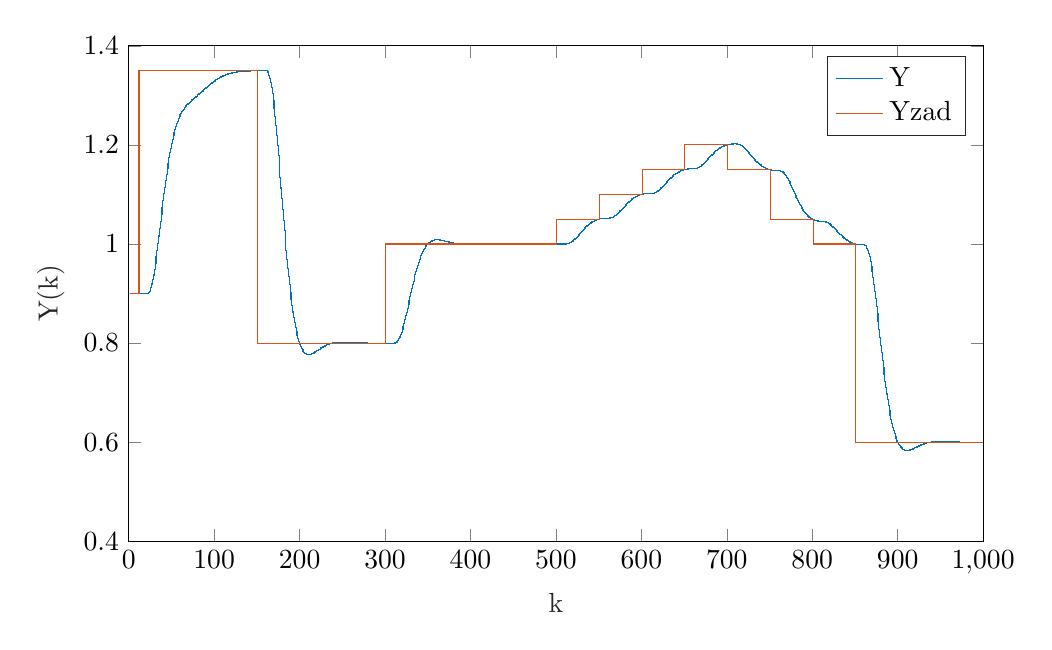
\begin{tikzpicture}

\begin{axis}[%
width=4.272in,
height=2.477in,
at={(0.717in,0.437in)},
scale only axis,
xmin=0,
xmax=1000,
xlabel style={font=\color{white!15!black}},
xlabel={k},
ymin=0.4,
ymax=1.4,
ylabel style={font=\color{white!15!black}},
ylabel={Y(k)},
axis background/.style={fill=white},
legend style={legend cell align=left, align=left, draw=white!15!black}
]
\addplot[const plot, color=mycolor1] table[row sep=crcr] {%
1	0.9\\
2	0.9\\
3	0.9\\
4	0.9\\
5	0.9\\
6	0.9\\
7	0.9\\
8	0.9\\
9	0.9\\
10	0.9\\
11	0.9\\
12	0.9\\
13	0.9\\
14	0.9\\
15	0.9\\
16	0.9\\
17	0.9\\
18	0.9\\
19	0.9\\
20	0.9\\
21	0.9\\
22	0.900294116514547\\
23	0.901377672137243\\
24	0.903608472825134\\
25	0.907228923890127\\
26	0.9123854723981\\
27	0.919145648584578\\
28	0.927512952188222\\
29	0.937411785305258\\
30	0.948630103279758\\
31	0.960892248466208\\
32	0.973958471831168\\
33	0.987620919466521\\
34	1.00170003505763\\
35	1.01604133706554\\
36	1.03051253335601\\
37	1.04500093960612\\
38	1.05941117107711\\
39	1.07366126360651\\
40	1.0876753898365\\
41	1.10138067532577\\
42	1.11470928306056\\
43	1.12760006628746\\
44	1.139999788024\\
45	1.15186392652357\\
46	1.16315710037831\\
47	1.17385315615688\\
48	1.18393496660014\\
49	1.19339399056229\\
50	1.20222964990763\\
51	1.21044857948802\\
52	1.21806379944857\\
53	1.22509384936093\\
54	1.23156191542108\\
55	1.23749497497565\\
56	1.24292297678336\\
57	1.24787807052561\\
58	1.25239389502051\\
59	1.2565049312512\\
60	1.26024592359205\\
61	1.26365137041636\\
62	1.26675508351972\\
63	1.26958981442629\\
64	1.27218694460375\\
65	1.27457623584319\\
66	1.27678563652116\\
67	1.27884113911145\\
68	1.28076668412191\\
69	1.2825841055682\\
70	1.28431311313528\\
71	1.28597130629941\\
72	1.28757421586869\\
73	1.28913536863361\\
74	1.29066637108766\\
75	1.29217700847028\\
76	1.29367535569141\\
77	1.29516789701017\\
78	1.29665965165446\\
79	1.29815430287688\\
80	1.29965432824308\\
81	1.30116112923615\\
82	1.3026751585343\\
83	1.30419604357584\\
84	1.3057227052648\\
85	1.30725347089137\\
86	1.30878618054325\\
87	1.31031828646757\\
88	1.31184694500742\\
89	1.31336910088415\\
90	1.31488156372544\\
91	1.31638107685235\\
92	1.31786437843518\\
93	1.31932825521059\\
94	1.3207695890209\\
95	1.32218539649263\\
96	1.32357286221555\\
97	1.32492936581787\\
98	1.32625250335715\\
99	1.32754010346288\\
100	1.32879023867503\\
101	1.33000123242475\\
102	1.33117166209976\\
103	1.33230035862817\\
104	1.33338640300178\\
105	1.33442912014381\\
106	1.33542807050695\\
107	1.33638303976667\\
108	1.33729402695205\\
109	1.3381612313325\\
110	1.33898503835436\\
111	1.33976600489635\\
112	1.34050484408828\\
113	1.34120240991269\\
114	1.34185968178528\\
115	1.34247774928673\\
116	1.34305779719628\\
117	1.34360109095607\\
118	1.34410896267491\\
119	1.34458279776129\\
120	1.34502402225908\\
121	1.34543409094269\\
122	1.34581447621386\\
123	1.34616665782864\\
124	1.34649211347068\\
125	1.34679231017646\\
126	1.34706869660806\\
127	1.3473226961609\\
128	1.34755570088646\\
129	1.34776906620396\\
130	1.34796410636957\\
131	1.34814209066787\\
132	1.34830424028646\\
133	1.34845172583266\\
134	1.34858566544892\\
135	1.34870712348267\\
136	1.34881710966603\\
137	1.34891657876016\\
138	1.34900643062015\\
139	1.34908751063686\\
140	1.34916061051323\\
141	1.34922646933442\\
142	1.3492857748925\\
143	1.34933916522847\\
144	1.34938723035671\\
145	1.34943051413849\\
146	1.34946951627427\\
147	1.34950469438609\\
148	1.34953646616398\\
149	1.34956521155271\\
150	1.34959127495727\\
151	1.34961496744762\\
152	1.34963656894576\\
153	1.34965633037978\\
154	1.3496744757918\\
155	1.34969120438857\\
156	1.34970669252501\\
157	1.34972109561301\\
158	1.34973454994895\\
159	1.34974717445504\\
160	1.34975907233087\\
161	1.34941085687259\\
162	1.34809721013734\\
163	1.34538087874472\\
164	1.34096564449809\\
165	1.33467256263711\\
166	1.32641913453473\\
167	1.31620111429493\\
168	1.30407667771978\\
169	1.29015270798078\\
170	1.27457297546643\\
171	1.25750801004079\\
172	1.23914648264038\\
173	1.21968793001971\\
174	1.19933667174922\\
175	1.17829678246421\\
176	1.15676799501917\\
177	1.13494242175846\\
178	1.1130019916875\\
179	1.09111651102049\\
180	1.06944226347773\\
181	1.04812107488073\\
182	1.02727977411326\\
183	1.00702998943417\\
184	0.987468225494207\\
185	0.968676172265581\\
186	0.950721202477258\\
187	0.933657019095788\\
188	0.917524418929562\\
189	0.902352142592282\\
190	0.888157784863519\\
191	0.874948742953708\\
192	0.862723183339262\\
193	0.851471010700762\\
194	0.841174825092262\\
195	0.831810855810348\\
196	0.82334986253478\\
197	0.815757996194185\\
198	0.808997613602381\\
199	0.803028041519588\\
200	0.797806287163761\\
201	0.793287693220414\\
202	0.789426536394352\\
203	0.786176569402659\\
204	0.783491507037039\\
205	0.781325457536305\\
206	0.779633301017144\\
207	0.778371017123319\\
208	0.777495964379798\\
209	0.776967113987836\\
210	0.776745240978338\\
211	0.776793075761662\\
212	0.777075419179937\\
213	0.777559224189683\\
214	0.778213647284455\\
215	0.779010072715274\\
216	0.779922112486051\\
217	0.780925584997045\\
218	0.781998475086101\\
219	0.783120878079066\\
220	0.784274930311022\\
221	0.785444728421977\\
222	0.786616239567437\\
223	0.787777204518257\\
224	0.788917035457632\\
225	0.790026710117992\\
226	0.791098663738463\\
227	0.79212668016594\\
228	0.793105783270783\\
229	0.794032129702656\\
230	0.794902903873827\\
231	0.795716215926865\\
232	0.796471003321598\\
233	0.797166936562554\\
234	0.797804329483172\\
235	0.798384054406773\\
236	0.79890746241659\\
237	0.799376308887865\\
238	0.799792684363997\\
239	0.800158950795556\\
240	0.800477683105451\\
241	0.800751615995202\\
242	0.800983595865743\\
243	0.801176537691073\\
244	0.801333386653912\\
245	0.801457084328861\\
246	0.80155053918002\\
247	0.80161660112607\\
248	0.801658039916072\\
249	0.801677527053314\\
250	0.801677621001906\\
251	0.80166075541122\\
252	0.801629230096269\\
253	0.801585204517332\\
254	0.801530693509293\\
255	0.801467565019919\\
256	0.801397539626374\\
257	0.8013221916111\\
258	0.801242951389779\\
259	0.801161109095687\\
260	0.80107781913782\\
261	0.800994105563417\\
262	0.800910868068794\\
263	0.800828888515532\\
264	0.800748837822072\\
265	0.800671283113318\\
266	0.80059669502313\\
267	0.800525455056271\\
268	0.800457862927585\\
269	0.800394143806793\\
270	0.800334455407294\\
271	0.80027889486669\\
272	0.800227505375505\\
273	0.80018028251856\\
274	0.800137180300902\\
275	0.800098116836904\\
276	0.80006297968727\\
277	0.80003163083417\\
278	0.80000391128963\\
279	0.799979645336647\\
280	0.79995864440625\\
281	0.799940710597061\\
282	0.799925639846678\\
283	0.799913224766554\\
284	0.799903257153999\\
285	0.799895530196489\\
286	0.799889840384652\\
287	0.79988598915122\\
288	0.79988378425381\\
289	0.799883040919761\\
290	0.799883582771368\\
291	0.799885242549763\\
292	0.799887862655449\\
293	0.799891295523069\\
294	0.799895403847485\\
295	0.799900060677572\\
296	0.799905149393431\\
297	0.799910563581925\\
298	0.799916206824604\\
299	0.799921992411191\\
300	0.79992784299093\\
301	0.799933690173148\\
302	0.799939474087513\\
303	0.799945142913531\\
304	0.799950652387971\\
305	0.799955965298018\\
306	0.79996105096716\\
307	0.799965884739987\\
308	0.799970447471342\\
309	0.799974725024543\\
310	0.799978707782728\\
311	0.800113108627651\\
312	0.800598068960049\\
313	0.801592614839385\\
314	0.803204485905693\\
315	0.805498776062916\\
316	0.808505507084122\\
317	0.812226244428545\\
318	0.816639854010352\\
319	0.821707489252869\\
320	0.8273768893484\\
321	0.833586062093558\\
322	0.840266417872426\\
323	0.847345415220667\\
324	0.85474877284211\\
325	0.862402297896742\\
326	0.870233375776588\\
327	0.878172162383659\\
328	0.886152516079111\\
329	0.894112702948393\\
330	0.901995905792165\\
331	0.909750564279888\\
332	0.917330570968891\\
333	0.924695345376023\\
334	0.931809805974155\\
335	0.93864425785621\\
336	0.945174211851382\\
337	0.951380149181723\\
338	0.957247243944936\\
339	0.962765054119195\\
340	0.967927190549915\\
341	0.972730972113401\\
342	0.977177074100855\\
343	0.981269175821086\\
344	0.985013612474418\\
345	0.988419035497369\\
346	0.991496084811306\\
347	0.994257075722777\\
348	0.996715702612773\\
349	0.998886761011565\\
350	1.00078588917971\\
351	1.00242932989958\\
352	1.00383371282038\\
353	1.00501585738906\\
354	1.00599259613464\\
355	1.00678061785159\\
356	1.00739633004338\\
357	1.00785573983812\\
358	1.00817435246987\\
359	1.00836708632869\\
360	1.00844820351702\\
361	1.00843125480609\\
362	1.00832903786192\\
363	1.00815356760252\\
364	1.00791605755481\\
365	1.00762691109883\\
366	1.00729572151627\\
367	1.00693127979828\\
368	1.00654158921257\\
369	1.00613388568019\\
370	1.00571466306682\\
371	1.00528970255123\\
372	1.0048641052926\\
373	1.00444232767926\\
374	1.00402821850151\\
375	1.00362505745183\\
376	1.00323559441415\\
377	1.00286208906166\\
378	1.00250635033762\\
379	1.00216977544673\\
380	1.00185338803457\\
381	1.00155787528047\\
382	1.00128362367302\\
383	1.0010307532791\\
384	1.00079915035529\\
385	1.00058849818556\\
386	1.00039830606098\\
387	1.00022793634591\\
388	1.00007662960115\\
389	0.999943527757286\\
390	0.999827695351714\\
391	0.999728138860308\\
392	0.999643824169933\\
393	0.999573692250594\\
394	0.999516673096677\\
395	0.999471698015319\\
396	0.99943771034666\\
397	0.99941367470581\\
398	0.99939858483987\\
399	0.999391470195536\\
400	0.999391401293721\\
401	0.999397494007493\\
402	0.999408912838561\\
403	0.999424873285586\\
404	0.999444643395035\\
405	0.99946754458209\\
406	0.999492951805455\\
407	0.99952029317561\\
408	0.999549049071845\\
409	0.999578750839188\\
410	0.999608979131592\\
411	0.999639361962924\\
412	0.999669572522492\\
413	0.999699326807022\\
414	0.999728381116342\\
415	0.99975652945539\\
416	0.999783600880767\\
417	0.999809456825756\\
418	0.999833988433706\\
419	0.999857113925763\\
420	0.999878776025359\\
421	0.999898939458428\\
422	0.999917588545168\\
423	0.99993472489626\\
424	0.999950365223726\\
425	0.999964539274225\\
426	0.999977287890286\\
427	0.999988661203061\\
428	0.999998716958332\\
429	1.00000751897599\\
430	1.00001513574178\\
431	1.00002163912895\\
432	1.0000271032464\\
433	1.00003160340906\\
434	1.00003521522565\\
435	1.00003801379813\\
436	1.00004007302704\\
437	1.00004146501635\\
438	1.00004225957142\\
439	1.00004252378332\\
440	1.00004232169302\\
441	1.00004171402855\\
442	1.00004075800896\\
443	1.00003950720831\\
444	1.00003801147376\\
445	1.00003631689162\\
446	1.00003446579588\\
447	1.00003249681345\\
448	1.00003044494139\\
449	1.00002834165111\\
450	1.00002621501505\\
451	1.00002408985194\\
452	1.00002198788652\\
453	1.0000199279206\\
454	1.00001792601194\\
455	1.00001599565848\\
456	1.00001414798502\\
457	1.00001239193046\\
458	1.0000107344333\\
459	1.00000918061396\\
460	1.00000773395219\\
461	1.0000063964586\\
462	1.00000516883908\\
463	1.00000405065131\\
464	1.00000304045287\\
465	1.00000213594024\\
466	1.00000133407857\\
467	1.0000006312219\\
468	1.00000002322388\\
469	0.999999505538959\\
470	0.999999073314239\\
471	0.999998721472246\\
472	0.999998444784926\\
473	0.999998237939264\\
474	0.999998095594971\\
475	0.999998012434755\\
476	0.999997983207711\\
477	0.999998002766423\\
478	0.999998066098394\\
479	0.999998168352428\\
480	0.999998304860518\\
481	0.999998471155723\\
482	0.999998662986464\\
483	0.999998876327582\\
484	0.999999107388509\\
485	0.999999352618815\\
486	0.999999608711408\\
487	0.999999872566443\\
488	1.00000014123429\\
489	1.00000041188424\\
490	1.00000068179239\\
491	1.00000094834308\\
492	1.00000120903957\\
493	1.00000146152039\\
494	1.0000017035784\\
495	1.00000193318063\\
496	1.00000214848696\\
497	1.00000234786669\\
498	1.00000252991207\\
499	1.00000269344826\\
500	1.00000283753951\\
501	1.00000296149147\\
502	1.00000306484969\\
503	1.00000314739463\\
504	1.00000320913329\\
505	1.00000325028805\\
506	1.00000327128291\\
507	1.00000327272772\\
508	1.00000325540068\\
509	1.00000322022967\\
510	1.00000316827269\\
511	1.00003578031061\\
512	1.00015609344539\\
513	1.00040386522285\\
514	1.00080603094572\\
515	1.00137886392159\\
516	1.00212986893582\\
517	1.00305943627207\\
518	1.00416228096546\\
519	1.00542868962182\\
520	1.00684559503355\\
521	1.00839749693435\\
522	1.01006724553656\\
523	1.0118367029594\\
524	1.0136872962663\\
525	1.01560047456647\\
526	1.01755808148502\\
527	1.01954265325555\\
528	1.02153765172792\\
529	1.02352764070252\\
530	1.02549841319404\\
531	1.02743707648395\\
532	1.02933210113779\\
533	1.03117333953395\\
534	1.03295201887245\\
535	1.03466071309913\\
536	1.0362932976918\\
537	1.03784489080469\\
538	1.03931178385537\\
539	1.04069136425995\\
540	1.041982032677\\
541	1.04318311680513\\
542	1.0442947834918\\
543	1.04531795065068\\
544	1.04625420024854\\
545	1.04710569341003\\
546	1.04787508849755\\
547	1.04856546285227\\
548	1.04918023873001\\
549	1.04972311383068\\
550	1.05019799670148\\
551	1.05060894718961\\
552	1.05096012203048\\
553	1.0512557255796\\
554	1.05149996563024\\
555	1.05169701420357\\
556	1.05185097315176\\
557	1.0519658443774\\
558	1.05204550444292\\
559	1.05209368332105\\
560	1.05211394702108\\
561	1.05214236342728\\
562	1.05223716846\\
563	1.05244112279393\\
564	1.05278396451621\\
565	1.05328456719078\\
566	1.0539528333485\\
567	1.05479135046415\\
568	1.05579683385534\\
569	1.05696137859957\\
570	1.05827354047581\\
571	1.05971926406392\\
572	1.06128267445077\\
573	1.06294674747214\\
574	1.0646938720443\\
575	1.0665063168912\\
576	1.06836661283707\\
577	1.07025786079823\\
578	1.07216397466046\\
579	1.07406986736026\\
580	1.07596158769227\\
581	1.0778264146336\\
582	1.07965291530327\\
583	1.0814309720566\\
584	1.08315178364474\\
585	1.08480784484641\\
586	1.08639290849673\\
587	1.08790193339614\\
588	1.0893310211759\\
589	1.09067734482446\\
590	1.09193907123851\\
591	1.09311527985135\\
592	1.09420587910787\\
593	1.09521152229793\\
594	1.09613352402672\\
595	1.09697377838994\\
596	1.09773467973206\\
597	1.09841904669629\\
598	1.09903005012335\\
599	1.09957114522158\\
600	1.10004600831259\\
601	1.10045847835246\\
602	1.10081250333823\\
603	1.10111209163103\\
604	1.10136126816087\\
605	1.10156403542143\\
606	1.10172433911644\\
607	1.10184603828087\\
608	1.10193287966935\\
609	1.10198847618074\\
610	1.1020162890701\\
611	1.10205229329991\\
612	1.10215464315511\\
613	1.10236602836952\\
614	1.10271612615802\\
615	1.10322375863172\\
616	1.10389878562491\\
617	1.10474376000371\\
618	1.10575536989859\\
619	1.1069256899638\\
620	1.10824326167536\\
621	1.109694020806\\
622	1.11126208852957\\
623	1.11293044108737\\
624	1.11468147157289\\
625	1.11649745614264\\
626	1.11836093582449\\
627	1.12025502405799\\
628	1.12216364915361\\
629	1.12407173998921\\
630	1.1259653624657\\
631	1.12783181351205\\
632	1.12965967875714\\
633	1.13143885936686\\
634	1.13316057297599\\
635	1.13481733311985\\
636	1.13640291108978\\
637	1.1379122836934\\
638	1.13934156999478\\
639	1.14068795973701\\
640	1.14194963580943\\
641	1.14312569281039\\
642	1.14421605347329\\
643	1.14522138446605\\
644	1.14614301284105\\
645	1.14698284420186\\
646	1.14774328346362\\
647	1.14842715891443\\
648	1.14903765013333\\
649	1.14957822018654\\
650	1.15005255240473\\
651	1.15046449194051\\
652	1.15081799221485\\
653	1.15111706628294\\
654	1.15136574308365\\
655	1.15156802848036\\
656	1.15172787095395\\
657	1.15184913177075\\
658	1.15193555941733\\
659	1.15199076807055\\
660	1.15201821985389\\
661	1.15205389023146\\
662	1.15215593366411\\
663	1.15236703977494\\
664	1.15271688541847\\
665	1.15322429213049\\
666	1.15389911898745\\
667	1.15474391794508\\
668	1.15575537609858\\
669	1.15692556696731\\
670	1.15824303081571\\
671	1.15969370214888\\
672	1.16126170083551\\
673	1.16293000179052\\
674	1.16468099677429\\
675	1.16649696061592\\
676	1.1683604330325\\
677	1.17025452617863\\
678	1.17216316711353\\
679	1.17407128350409\\
680	1.17596494008597\\
681	1.17783143267309\\
682	1.17965934583302\\
683	1.18143857972691\\
684	1.1831603510433\\
685	1.18481717243125\\
686	1.18640281435655\\
687	1.18791225285303\\
688	1.18934160624835\\
689	1.19068806357891\\
690	1.1919498070539\\
691	1.19312593061852\\
692	1.19421635638266\\
693	1.19522175042445\\
694	1.19614343924502\\
695	1.19698332794008\\
696	1.19774382096513\\
697	1.19842774620086\\
698	1.19903828287461\\
699	1.19957889375904\\
700	1.200053261951\\
701	1.20046523242958\\
702	1.20081875850215\\
703	1.201117853169\\
704	1.2013665453707\\
705	1.20156884102613\\
706	1.20172868872206\\
707	1.20184994987716\\
708	1.20193637317239\\
709	1.20199157301641\\
710	1.20201901179702\\
711	1.20198930604474\\
712	1.20185053884729\\
713	1.2015658877248\\
714	1.20111116202928\\
715	1.20047263985674\\
716	1.1996451739209\\
717	1.19863053881355\\
718	1.19743599472412\\
719	1.19607304505432\\
720	1.19455636747962\\
721	1.19290289991037\\
722	1.19113106451879\\
723	1.18926011454727\\
724	1.18730959001805\\
725	1.18529886974211\\
726	1.1832468081896\\
727	1.18117144684877\\
728	1.17908979067478\\
729	1.1770176411238\\
730	1.17496947808867\\
731	1.17295838380744\\
732	1.17099600251009\\
733	1.16909253020824\\
734	1.16725672962038\\
735	1.16549596576644\\
736	1.16381625826268\\
737	1.16222234679554\\
738	1.16071776668587\\
739	1.15930493184569\\
740	1.15798522276706\\
741	1.15675907750277\\
742	1.15562608388978\\
743	1.15458507153031\\
744	1.15363420228465\\
745	1.1527710582446\\
746	1.15199272634967\\
747	1.15129587898082\\
748	1.15067685001972\\
749	1.15013170599731\\
750	1.14965631207458\\
751	1.14924639270258\\
752	1.1488975868987\\
753	1.14860549815345\\
754	1.14836573904772\\
755	1.14817397071502\\
756	1.14802593732861\\
757	1.14791749582975\\
758	1.14784464114179\\
759	1.14780352713645\\
760	1.14779048363411\\
761	1.14773667050402\\
762	1.14752873437521\\
763	1.14708408721768\\
764	1.14634599575766\\
765	1.14527926252654\\
766	1.14386643824394\\
767	1.14210451115961\\
768	1.14000202424195\\
769	1.13757657578996\\
770	1.13485266323774\\
771	1.13185983368042\\
772	1.12863110803361\\
773	1.12520164879175\\
774	1.12160764411627\\
775	1.11788538349448\\
776	1.11407050249635\\
777	1.11019737624268\\
778	1.10629864310592\\
779	1.10240484191414\\
780	1.09854414753265\\
781	1.09474219117273\\
782	1.09102195313217\\
783	1.08740371692013\\
784	1.08390507486641\\
785	1.08054097637101\\
786	1.07732381092114\\
787	1.07426351888544\\
788	1.07136772392755\\
789	1.06864188163882\\
790	1.06608943966258\\
791	1.06371200520922\\
792	1.06150951643237\\
793	1.0594804146545\\
794	1.05762181490019\\
795	1.05592967261866\\
796	1.05439894485807\\
797	1.05302374449564\\
798	1.05179748643082\\
799	1.05071302491912\\
800	1.04976278146105\\
801	1.0489388628692\\
802	1.04823316931694\\
803	1.04763749232821\\
804	1.04714360280082\\
805	1.04674332926737\\
806	1.04642862669131\\
807	1.04619163617111\\
808	1.04602473598601\\
809	1.04592058446313\\
810	1.04587215517974\\
811	1.04584008542482\\
812	1.04576302107778\\
813	1.04559526794072\\
814	1.04530434441273\\
815	1.04486882630673\\
816	1.0442764540506\\
817	1.04352247546403\\
818	1.04260819991849\\
819	1.04153974201512\\
820	1.04032693499218\\
821	1.03898239593352\\
822	1.03752072651988\\
823	1.03595783457017\\
824	1.03431036298068\\
825	1.03259521390391\\
826	1.03082915713022\\
827	1.02902851265826\\
828	1.02720889837378\\
829	1.02538503461185\\
830	1.02357059816123\\
831	1.02177811898968\\
832	1.02001891363055\\
833	1.0183030497795\\
834	1.01663933721007\\
835	1.01503534063182\\
836	1.01349741058852\\
837	1.01203072891995\\
838	1.01063936572418\\
839	1.00932634513135\\
840	1.00809371752159\\
841	1.00694263612715\\
842	1.0058734362384\\
843	1.00488571548796\\
844	1.00397841391784\\
845	1.00314989274332\\
846	1.00239801091495\\
847	1.00172019874887\\
848	1.00111352804596\\
849	1.00057477825451\\
850	1.00010049834916\\
851	0.999687064203038\\
852	0.999330731320606\\
853	0.999027682877226\\
854	0.998774073078913\\
855	0.998566065912642\\
856	0.998399869405424\\
857	0.998271765549794\\
858	0.998178136084931\\
859	0.998115484347303\\
860	0.998080453423459\\
861	0.997808403949026\\
862	0.9968560126657\\
863	0.994902367843835\\
864	0.991729316508009\\
865	0.987204185766197\\
866	0.981264636175145\\
867	0.973905428807323\\
868	0.965166908774937\\
869	0.955125026767598\\
870	0.943882736974955\\
871	0.931562624852945\\
872	0.91830063177372\\
873	0.904240755863747\\
874	0.88953061944356\\
875	0.874317803573822\\
876	0.858746859403313\\
877	0.842956914405544\\
878	0.827079799267668\\
879	0.811238628231625\\
880	0.795546772145953\\
881	0.780107169421624\\
882	0.765011925543285\\
883	0.750342156809032\\
884	0.73616803859263\\
885	0.722549022673013\\
886	0.709534192084318\\
887	0.697162725539485\\
888	0.685464446761015\\
889	0.674460437063668\\
890	0.6641636923075\\
891	0.654579807858442\\
892	0.645707677486751\\
893	0.63754019421568\\
894	0.630064943017309\\
895	0.623264876952465\\
896	0.617118969879404\\
897	0.611602840223035\\
898	0.6066893415141\\
899	0.602349116486525\\
900	0.59855111247136\\
901	0.595263056657044\\
902	0.592451890507496\\
903	0.590084163250694\\
904	0.588126384879437\\
905	0.586545339550991\\
906	0.585308360640995\\
907	0.584383569006741\\
908	0.583740076252425\\
909	0.583348154970749\\
910	0.583179378067695\\
911	0.58320672936582\\
912	0.583404687731603\\
913	0.58374928698898\\
914	0.584218153868966\\
915	0.5847905262084\\
916	0.585447253553174\\
917	0.586170782246545\\
918	0.586945126994361\\
919	0.587755830799313\\
920	0.588589915048215\\
921	0.589435821422277\\
922	0.590283347182303\\
923	0.591123575260795\\
924	0.591948800472456\\
925	0.592752453035174\\
926	0.593529020476229\\
927	0.594273968884433\\
928	0.594983664358767\\
929	0.595655295398792\\
930	0.596286796881999\\
931	0.596876776178862\\
932	0.597424441867899\\
933	0.597929535430715\\
934	0.598392266230916\\
935	0.598813250010934\\
936	0.599193451077201\\
937	0.599534128305149\\
938	0.599836785016274\\
939	0.600103122719442\\
940	0.600334998694929\\
941	0.600534387363933\\
942	0.600703345355553\\
943	0.600843980157237\\
944	0.600958422213043\\
945	0.601048800316486\\
946	0.601117220130885\\
947	0.601165745659697\\
948	0.601196383481943\\
949	0.601211069563274\\
950	0.601211658451087\\
951	0.60119991466221\\
952	0.601177506073656\\
953	0.60114599913059\\
954	0.601106855690737\\
955	0.60106143133067\\
956	0.601010974946675\\
957	0.600956629491378\\
958	0.600899433695659\\
959	0.600840324633764\\
960	0.600780140998936\\
961	0.600719626966501\\
962	0.600659436530929\\
963	0.60060013821294\\
964	0.600542220042106\\
965	0.600486094729548\\
966	0.600432104954201\\
967	0.600380528694605\\
968	0.600331584546339\\
969	0.600285436972889\\
970	0.600242201445031\\
971	0.600201949430571\\
972	0.600164713202661\\
973	0.600130490440698\\
974	0.600099248603238\\
975	0.600070929057229\\
976	0.60004545095232\\
977	0.600022714832993\\
978	0.600002605984839\\
979	0.599984997514435\\
980	0.599969753165077\\
981	0.599956729873027\\
982	0.599945780070975\\
983	0.599936753747175\\
984	0.599929500270096\\
985	0.599923869989609\\
986	0.599919715626601\\
987	0.599916893472832\\
988	0.59991526440951\\
989	0.599914694746188\\
990	0.599915056895011\\
991	0.599916229895008\\
992	0.599918099800647\\
993	0.599920559948376\\
994	0.599923511114289\\
995	0.599926861575429\\
996	0.59993052708657\\
997	0.599934430783654\\
998	0.59993850302431\\
999	0.599942681175208\\
1000	0.599946909355247\\
};
\addlegendentry{Y}

\addplot[const plot, color=mycolor2] table[row sep=crcr] {%
1	0.9\\
2	0.9\\
3	0.9\\
4	0.9\\
5	0.9\\
6	0.9\\
7	0.9\\
8	0.9\\
9	0.9\\
10	0.9\\
11	0.9\\
12	1.35\\
13	1.35\\
14	1.35\\
15	1.35\\
16	1.35\\
17	1.35\\
18	1.35\\
19	1.35\\
20	1.35\\
21	1.35\\
22	1.35\\
23	1.35\\
24	1.35\\
25	1.35\\
26	1.35\\
27	1.35\\
28	1.35\\
29	1.35\\
30	1.35\\
31	1.35\\
32	1.35\\
33	1.35\\
34	1.35\\
35	1.35\\
36	1.35\\
37	1.35\\
38	1.35\\
39	1.35\\
40	1.35\\
41	1.35\\
42	1.35\\
43	1.35\\
44	1.35\\
45	1.35\\
46	1.35\\
47	1.35\\
48	1.35\\
49	1.35\\
50	1.35\\
51	1.35\\
52	1.35\\
53	1.35\\
54	1.35\\
55	1.35\\
56	1.35\\
57	1.35\\
58	1.35\\
59	1.35\\
60	1.35\\
61	1.35\\
62	1.35\\
63	1.35\\
64	1.35\\
65	1.35\\
66	1.35\\
67	1.35\\
68	1.35\\
69	1.35\\
70	1.35\\
71	1.35\\
72	1.35\\
73	1.35\\
74	1.35\\
75	1.35\\
76	1.35\\
77	1.35\\
78	1.35\\
79	1.35\\
80	1.35\\
81	1.35\\
82	1.35\\
83	1.35\\
84	1.35\\
85	1.35\\
86	1.35\\
87	1.35\\
88	1.35\\
89	1.35\\
90	1.35\\
91	1.35\\
92	1.35\\
93	1.35\\
94	1.35\\
95	1.35\\
96	1.35\\
97	1.35\\
98	1.35\\
99	1.35\\
100	1.35\\
101	1.35\\
102	1.35\\
103	1.35\\
104	1.35\\
105	1.35\\
106	1.35\\
107	1.35\\
108	1.35\\
109	1.35\\
110	1.35\\
111	1.35\\
112	1.35\\
113	1.35\\
114	1.35\\
115	1.35\\
116	1.35\\
117	1.35\\
118	1.35\\
119	1.35\\
120	1.35\\
121	1.35\\
122	1.35\\
123	1.35\\
124	1.35\\
125	1.35\\
126	1.35\\
127	1.35\\
128	1.35\\
129	1.35\\
130	1.35\\
131	1.35\\
132	1.35\\
133	1.35\\
134	1.35\\
135	1.35\\
136	1.35\\
137	1.35\\
138	1.35\\
139	1.35\\
140	1.35\\
141	1.35\\
142	1.35\\
143	1.35\\
144	1.35\\
145	1.35\\
146	1.35\\
147	1.35\\
148	1.35\\
149	1.35\\
150	1.35\\
151	0.8\\
152	0.8\\
153	0.8\\
154	0.8\\
155	0.8\\
156	0.8\\
157	0.8\\
158	0.8\\
159	0.8\\
160	0.8\\
161	0.8\\
162	0.8\\
163	0.8\\
164	0.8\\
165	0.8\\
166	0.8\\
167	0.8\\
168	0.8\\
169	0.8\\
170	0.8\\
171	0.8\\
172	0.8\\
173	0.8\\
174	0.8\\
175	0.8\\
176	0.8\\
177	0.8\\
178	0.8\\
179	0.8\\
180	0.8\\
181	0.8\\
182	0.8\\
183	0.8\\
184	0.8\\
185	0.8\\
186	0.8\\
187	0.8\\
188	0.8\\
189	0.8\\
190	0.8\\
191	0.8\\
192	0.8\\
193	0.8\\
194	0.8\\
195	0.8\\
196	0.8\\
197	0.8\\
198	0.8\\
199	0.8\\
200	0.8\\
201	0.8\\
202	0.8\\
203	0.8\\
204	0.8\\
205	0.8\\
206	0.8\\
207	0.8\\
208	0.8\\
209	0.8\\
210	0.8\\
211	0.8\\
212	0.8\\
213	0.8\\
214	0.8\\
215	0.8\\
216	0.8\\
217	0.8\\
218	0.8\\
219	0.8\\
220	0.8\\
221	0.8\\
222	0.8\\
223	0.8\\
224	0.8\\
225	0.8\\
226	0.8\\
227	0.8\\
228	0.8\\
229	0.8\\
230	0.8\\
231	0.8\\
232	0.8\\
233	0.8\\
234	0.8\\
235	0.8\\
236	0.8\\
237	0.8\\
238	0.8\\
239	0.8\\
240	0.8\\
241	0.8\\
242	0.8\\
243	0.8\\
244	0.8\\
245	0.8\\
246	0.8\\
247	0.8\\
248	0.8\\
249	0.8\\
250	0.8\\
251	0.8\\
252	0.8\\
253	0.8\\
254	0.8\\
255	0.8\\
256	0.8\\
257	0.8\\
258	0.8\\
259	0.8\\
260	0.8\\
261	0.8\\
262	0.8\\
263	0.8\\
264	0.8\\
265	0.8\\
266	0.8\\
267	0.8\\
268	0.8\\
269	0.8\\
270	0.8\\
271	0.8\\
272	0.8\\
273	0.8\\
274	0.8\\
275	0.8\\
276	0.8\\
277	0.8\\
278	0.8\\
279	0.8\\
280	0.8\\
281	0.8\\
282	0.8\\
283	0.8\\
284	0.8\\
285	0.8\\
286	0.8\\
287	0.8\\
288	0.8\\
289	0.8\\
290	0.8\\
291	0.8\\
292	0.8\\
293	0.8\\
294	0.8\\
295	0.8\\
296	0.8\\
297	0.8\\
298	0.8\\
299	0.8\\
300	0.8\\
301	1\\
302	1\\
303	1\\
304	1\\
305	1\\
306	1\\
307	1\\
308	1\\
309	1\\
310	1\\
311	1\\
312	1\\
313	1\\
314	1\\
315	1\\
316	1\\
317	1\\
318	1\\
319	1\\
320	1\\
321	1\\
322	1\\
323	1\\
324	1\\
325	1\\
326	1\\
327	1\\
328	1\\
329	1\\
330	1\\
331	1\\
332	1\\
333	1\\
334	1\\
335	1\\
336	1\\
337	1\\
338	1\\
339	1\\
340	1\\
341	1\\
342	1\\
343	1\\
344	1\\
345	1\\
346	1\\
347	1\\
348	1\\
349	1\\
350	1\\
351	1\\
352	1\\
353	1\\
354	1\\
355	1\\
356	1\\
357	1\\
358	1\\
359	1\\
360	1\\
361	1\\
362	1\\
363	1\\
364	1\\
365	1\\
366	1\\
367	1\\
368	1\\
369	1\\
370	1\\
371	1\\
372	1\\
373	1\\
374	1\\
375	1\\
376	1\\
377	1\\
378	1\\
379	1\\
380	1\\
381	1\\
382	1\\
383	1\\
384	1\\
385	1\\
386	1\\
387	1\\
388	1\\
389	1\\
390	1\\
391	1\\
392	1\\
393	1\\
394	1\\
395	1\\
396	1\\
397	1\\
398	1\\
399	1\\
400	1\\
401	1\\
402	1\\
403	1\\
404	1\\
405	1\\
406	1\\
407	1\\
408	1\\
409	1\\
410	1\\
411	1\\
412	1\\
413	1\\
414	1\\
415	1\\
416	1\\
417	1\\
418	1\\
419	1\\
420	1\\
421	1\\
422	1\\
423	1\\
424	1\\
425	1\\
426	1\\
427	1\\
428	1\\
429	1\\
430	1\\
431	1\\
432	1\\
433	1\\
434	1\\
435	1\\
436	1\\
437	1\\
438	1\\
439	1\\
440	1\\
441	1\\
442	1\\
443	1\\
444	1\\
445	1\\
446	1\\
447	1\\
448	1\\
449	1\\
450	1\\
451	1\\
452	1\\
453	1\\
454	1\\
455	1\\
456	1\\
457	1\\
458	1\\
459	1\\
460	1\\
461	1\\
462	1\\
463	1\\
464	1\\
465	1\\
466	1\\
467	1\\
468	1\\
469	1\\
470	1\\
471	1\\
472	1\\
473	1\\
474	1\\
475	1\\
476	1\\
477	1\\
478	1\\
479	1\\
480	1\\
481	1\\
482	1\\
483	1\\
484	1\\
485	1\\
486	1\\
487	1\\
488	1\\
489	1\\
490	1\\
491	1\\
492	1\\
493	1\\
494	1\\
495	1\\
496	1\\
497	1\\
498	1\\
499	1\\
500	1\\
501	1.05\\
502	1.05\\
503	1.05\\
504	1.05\\
505	1.05\\
506	1.05\\
507	1.05\\
508	1.05\\
509	1.05\\
510	1.05\\
511	1.05\\
512	1.05\\
513	1.05\\
514	1.05\\
515	1.05\\
516	1.05\\
517	1.05\\
518	1.05\\
519	1.05\\
520	1.05\\
521	1.05\\
522	1.05\\
523	1.05\\
524	1.05\\
525	1.05\\
526	1.05\\
527	1.05\\
528	1.05\\
529	1.05\\
530	1.05\\
531	1.05\\
532	1.05\\
533	1.05\\
534	1.05\\
535	1.05\\
536	1.05\\
537	1.05\\
538	1.05\\
539	1.05\\
540	1.05\\
541	1.05\\
542	1.05\\
543	1.05\\
544	1.05\\
545	1.05\\
546	1.05\\
547	1.05\\
548	1.05\\
549	1.05\\
550	1.05\\
551	1.1\\
552	1.1\\
553	1.1\\
554	1.1\\
555	1.1\\
556	1.1\\
557	1.1\\
558	1.1\\
559	1.1\\
560	1.1\\
561	1.1\\
562	1.1\\
563	1.1\\
564	1.1\\
565	1.1\\
566	1.1\\
567	1.1\\
568	1.1\\
569	1.1\\
570	1.1\\
571	1.1\\
572	1.1\\
573	1.1\\
574	1.1\\
575	1.1\\
576	1.1\\
577	1.1\\
578	1.1\\
579	1.1\\
580	1.1\\
581	1.1\\
582	1.1\\
583	1.1\\
584	1.1\\
585	1.1\\
586	1.1\\
587	1.1\\
588	1.1\\
589	1.1\\
590	1.1\\
591	1.1\\
592	1.1\\
593	1.1\\
594	1.1\\
595	1.1\\
596	1.1\\
597	1.1\\
598	1.1\\
599	1.1\\
600	1.1\\
601	1.15\\
602	1.15\\
603	1.15\\
604	1.15\\
605	1.15\\
606	1.15\\
607	1.15\\
608	1.15\\
609	1.15\\
610	1.15\\
611	1.15\\
612	1.15\\
613	1.15\\
614	1.15\\
615	1.15\\
616	1.15\\
617	1.15\\
618	1.15\\
619	1.15\\
620	1.15\\
621	1.15\\
622	1.15\\
623	1.15\\
624	1.15\\
625	1.15\\
626	1.15\\
627	1.15\\
628	1.15\\
629	1.15\\
630	1.15\\
631	1.15\\
632	1.15\\
633	1.15\\
634	1.15\\
635	1.15\\
636	1.15\\
637	1.15\\
638	1.15\\
639	1.15\\
640	1.15\\
641	1.15\\
642	1.15\\
643	1.15\\
644	1.15\\
645	1.15\\
646	1.15\\
647	1.15\\
648	1.15\\
649	1.15\\
650	1.15\\
651	1.2\\
652	1.2\\
653	1.2\\
654	1.2\\
655	1.2\\
656	1.2\\
657	1.2\\
658	1.2\\
659	1.2\\
660	1.2\\
661	1.2\\
662	1.2\\
663	1.2\\
664	1.2\\
665	1.2\\
666	1.2\\
667	1.2\\
668	1.2\\
669	1.2\\
670	1.2\\
671	1.2\\
672	1.2\\
673	1.2\\
674	1.2\\
675	1.2\\
676	1.2\\
677	1.2\\
678	1.2\\
679	1.2\\
680	1.2\\
681	1.2\\
682	1.2\\
683	1.2\\
684	1.2\\
685	1.2\\
686	1.2\\
687	1.2\\
688	1.2\\
689	1.2\\
690	1.2\\
691	1.2\\
692	1.2\\
693	1.2\\
694	1.2\\
695	1.2\\
696	1.2\\
697	1.2\\
698	1.2\\
699	1.2\\
700	1.2\\
701	1.15\\
702	1.15\\
703	1.15\\
704	1.15\\
705	1.15\\
706	1.15\\
707	1.15\\
708	1.15\\
709	1.15\\
710	1.15\\
711	1.15\\
712	1.15\\
713	1.15\\
714	1.15\\
715	1.15\\
716	1.15\\
717	1.15\\
718	1.15\\
719	1.15\\
720	1.15\\
721	1.15\\
722	1.15\\
723	1.15\\
724	1.15\\
725	1.15\\
726	1.15\\
727	1.15\\
728	1.15\\
729	1.15\\
730	1.15\\
731	1.15\\
732	1.15\\
733	1.15\\
734	1.15\\
735	1.15\\
736	1.15\\
737	1.15\\
738	1.15\\
739	1.15\\
740	1.15\\
741	1.15\\
742	1.15\\
743	1.15\\
744	1.15\\
745	1.15\\
746	1.15\\
747	1.15\\
748	1.15\\
749	1.15\\
750	1.15\\
751	1.05\\
752	1.05\\
753	1.05\\
754	1.05\\
755	1.05\\
756	1.05\\
757	1.05\\
758	1.05\\
759	1.05\\
760	1.05\\
761	1.05\\
762	1.05\\
763	1.05\\
764	1.05\\
765	1.05\\
766	1.05\\
767	1.05\\
768	1.05\\
769	1.05\\
770	1.05\\
771	1.05\\
772	1.05\\
773	1.05\\
774	1.05\\
775	1.05\\
776	1.05\\
777	1.05\\
778	1.05\\
779	1.05\\
780	1.05\\
781	1.05\\
782	1.05\\
783	1.05\\
784	1.05\\
785	1.05\\
786	1.05\\
787	1.05\\
788	1.05\\
789	1.05\\
790	1.05\\
791	1.05\\
792	1.05\\
793	1.05\\
794	1.05\\
795	1.05\\
796	1.05\\
797	1.05\\
798	1.05\\
799	1.05\\
800	1.05\\
801	1\\
802	1\\
803	1\\
804	1\\
805	1\\
806	1\\
807	1\\
808	1\\
809	1\\
810	1\\
811	1\\
812	1\\
813	1\\
814	1\\
815	1\\
816	1\\
817	1\\
818	1\\
819	1\\
820	1\\
821	1\\
822	1\\
823	1\\
824	1\\
825	1\\
826	1\\
827	1\\
828	1\\
829	1\\
830	1\\
831	1\\
832	1\\
833	1\\
834	1\\
835	1\\
836	1\\
837	1\\
838	1\\
839	1\\
840	1\\
841	1\\
842	1\\
843	1\\
844	1\\
845	1\\
846	1\\
847	1\\
848	1\\
849	1\\
850	1\\
851	0.6\\
852	0.6\\
853	0.6\\
854	0.6\\
855	0.6\\
856	0.6\\
857	0.6\\
858	0.6\\
859	0.6\\
860	0.6\\
861	0.6\\
862	0.6\\
863	0.6\\
864	0.6\\
865	0.6\\
866	0.6\\
867	0.6\\
868	0.6\\
869	0.6\\
870	0.6\\
871	0.6\\
872	0.6\\
873	0.6\\
874	0.6\\
875	0.6\\
876	0.6\\
877	0.6\\
878	0.6\\
879	0.6\\
880	0.6\\
881	0.6\\
882	0.6\\
883	0.6\\
884	0.6\\
885	0.6\\
886	0.6\\
887	0.6\\
888	0.6\\
889	0.6\\
890	0.6\\
891	0.6\\
892	0.6\\
893	0.6\\
894	0.6\\
895	0.6\\
896	0.6\\
897	0.6\\
898	0.6\\
899	0.6\\
900	0.6\\
901	0.6\\
902	0.6\\
903	0.6\\
904	0.6\\
905	0.6\\
906	0.6\\
907	0.6\\
908	0.6\\
909	0.6\\
910	0.6\\
911	0.6\\
912	0.6\\
913	0.6\\
914	0.6\\
915	0.6\\
916	0.6\\
917	0.6\\
918	0.6\\
919	0.6\\
920	0.6\\
921	0.6\\
922	0.6\\
923	0.6\\
924	0.6\\
925	0.6\\
926	0.6\\
927	0.6\\
928	0.6\\
929	0.6\\
930	0.6\\
931	0.6\\
932	0.6\\
933	0.6\\
934	0.6\\
935	0.6\\
936	0.6\\
937	0.6\\
938	0.6\\
939	0.6\\
940	0.6\\
941	0.6\\
942	0.6\\
943	0.6\\
944	0.6\\
945	0.6\\
946	0.6\\
947	0.6\\
948	0.6\\
949	0.6\\
950	0.6\\
951	0.6\\
952	0.6\\
953	0.6\\
954	0.6\\
955	0.6\\
956	0.6\\
957	0.6\\
958	0.6\\
959	0.6\\
960	0.6\\
961	0.6\\
962	0.6\\
963	0.6\\
964	0.6\\
965	0.6\\
966	0.6\\
967	0.6\\
968	0.6\\
969	0.6\\
970	0.6\\
971	0.6\\
972	0.6\\
973	0.6\\
974	0.6\\
975	0.6\\
976	0.6\\
977	0.6\\
978	0.6\\
979	0.6\\
980	0.6\\
981	0.6\\
982	0.6\\
983	0.6\\
984	0.6\\
985	0.6\\
986	0.6\\
987	0.6\\
988	0.6\\
989	0.6\\
990	0.6\\
991	0.6\\
992	0.6\\
993	0.6\\
994	0.6\\
995	0.6\\
996	0.6\\
997	0.6\\
998	0.6\\
999	0.6\\
1000	0.6\\
};
\addlegendentry{Yzad}

\end{axis}
\end{tikzpicture}%
\caption{Wyjście DMC dla parametrów $N=80$, $N_u=20$, $\lambda=60$}
\end{figure}

\begin{equation}
E = 18,3800
\end{equation}

